\documentclass[twoside]{book}

% Packages required by doxygen
\usepackage{fixltx2e}
\usepackage{calc}
\usepackage{doxygen}
\usepackage[export]{adjustbox} % also loads graphicx
\usepackage{graphicx}
\usepackage[utf8]{inputenc}
\usepackage{makeidx}
\usepackage{multicol}
\usepackage{multirow}
\PassOptionsToPackage{warn}{textcomp}
\usepackage{textcomp}
\usepackage[nointegrals]{wasysym}
\usepackage[table]{xcolor}

% Font selection
\usepackage[T1]{fontenc}
\usepackage[scaled=.90]{helvet}
\usepackage{courier}
\usepackage{amssymb}
\usepackage{sectsty}
\renewcommand{\familydefault}{\sfdefault}
\allsectionsfont{%
  \fontseries{bc}\selectfont%
  \color{darkgray}%
}
\renewcommand{\DoxyLabelFont}{%
  \fontseries{bc}\selectfont%
  \color{darkgray}%
}
\newcommand{\+}{\discretionary{\mbox{\scriptsize$\hookleftarrow$}}{}{}}

% Page & text layout
\usepackage{geometry}
\geometry{%
  a4paper,%
  top=2.5cm,%
  bottom=2.5cm,%
  left=2.5cm,%
  right=2.5cm%
}
\tolerance=750
\hfuzz=15pt
\hbadness=750
\setlength{\emergencystretch}{15pt}
\setlength{\parindent}{0cm}
\setlength{\parskip}{3ex plus 2ex minus 2ex}
\makeatletter
\renewcommand{\paragraph}{%
  \@startsection{paragraph}{4}{0ex}{-1.0ex}{1.0ex}{%
    \normalfont\normalsize\bfseries\SS@parafont%
  }%
}
\renewcommand{\subparagraph}{%
  \@startsection{subparagraph}{5}{0ex}{-1.0ex}{1.0ex}{%
    \normalfont\normalsize\bfseries\SS@subparafont%
  }%
}
\makeatother

% Headers & footers
\usepackage{fancyhdr}
\pagestyle{fancyplain}
\fancyhead[LE]{\fancyplain{}{\bfseries\thepage}}
\fancyhead[CE]{\fancyplain{}{}}
\fancyhead[RE]{\fancyplain{}{\bfseries\leftmark}}
\fancyhead[LO]{\fancyplain{}{\bfseries\rightmark}}
\fancyhead[CO]{\fancyplain{}{}}
\fancyhead[RO]{\fancyplain{}{\bfseries\thepage}}
\fancyfoot[LE]{\fancyplain{}{}}
\fancyfoot[CE]{\fancyplain{}{}}
\fancyfoot[RE]{\fancyplain{}{\bfseries\scriptsize Generated by Doxygen }}
\fancyfoot[LO]{\fancyplain{}{\bfseries\scriptsize Generated by Doxygen }}
\fancyfoot[CO]{\fancyplain{}{}}
\fancyfoot[RO]{\fancyplain{}{}}
\renewcommand{\footrulewidth}{0.4pt}
\renewcommand{\chaptermark}[1]{%
  \markboth{#1}{}%
}
\renewcommand{\sectionmark}[1]{%
  \markright{\thesection\ #1}%
}

% Indices & bibliography
\usepackage{natbib}
\usepackage[titles]{tocloft}
\setcounter{tocdepth}{3}
\setcounter{secnumdepth}{5}
\makeindex

% Hyperlinks (required, but should be loaded last)
\usepackage{ifpdf}
\ifpdf
  \usepackage[pdftex,pagebackref=true]{hyperref}
\else
  \usepackage[ps2pdf,pagebackref=true]{hyperref}
\fi
\hypersetup{%
  colorlinks=true,%
  linkcolor=blue,%
  citecolor=blue,%
  unicode%
}

% Custom commands
\newcommand{\clearemptydoublepage}{%
  \newpage{\pagestyle{empty}\cleardoublepage}%
}

\usepackage{caption}
\captionsetup{labelsep=space,justification=centering,font={bf},singlelinecheck=off,skip=4pt,position=top}

%===== C O N T E N T S =====

\begin{document}

% Titlepage & ToC
\hypersetup{pageanchor=false,
             bookmarksnumbered=true,
             pdfencoding=unicode
            }
\pagenumbering{alph}
\begin{titlepage}
\vspace*{7cm}
\begin{center}%
{\Large Drone Search \& Rescue System }\\
\vspace*{1cm}
{\large Generated by Doxygen 1.8.13}\\
\end{center}
\end{titlepage}
\clearemptydoublepage
\pagenumbering{roman}
\tableofcontents
\clearemptydoublepage
\pagenumbering{arabic}
\hypersetup{pageanchor=true}

%--- Begin generated contents ---
\chapter{Droners Index Page}
\label{index}\hypertarget{index}{}\hypertarget{index_intro_sec}{}\section{The Droner\textquotesingle{}s Drone Project}\label{index_intro_sec}
This is a project developed in C++ by Gabe Fendrich, Fletcher Gornick, Peyton Johnson, Luke Wiskus and Jason Woitalla. The purpose of this project was to solve a problem presented in our computer science class. We have been given a simulation where a drone, robot, hospital and recharge station are present. Our program runs the backend of this simulation to move the drone with the end goal of locating the robot. We do this using two major subsystems. Fist we have the \href{image_processing_description.html}{\tt image processing subsystem} and next we have the \href{simulation_description.html}{\tt simulation backend subsystem}.

To actually run the project, you can view our \href{getting_started.html}{\tt getting started with the libraries page} which details how to build, the code. It also links to our github \href{https://github.umn.edu/umn-csci-3081-f21/repo-team-0}{\tt https\+://github.\+umn.\+edu/umn-\/csci-\/3081-\/f21/repo-\/team-\/0} which has more information on cloneing and contributing to the project. This project is open source, so if you would like to contribute to it please read our \href{how_to_contribute.html}{\tt How to Contribute page}.

Another tool we used for this project was deploying it to docker. More information can be seen on our, \href{how_to_use_docker.html}{\tt how we use docker page}. Docker is a container based development environment that allows us to build this project with little overhead because it just contains the dependencies we need. The project can then be built or contributed to using docker.

Once our docker container is running, you can view the simulation in action by going to \href{http://127.0.0.1:8081/}{\tt http\+://127.\+0.\+0.\+1\+:8081/} . Or go to \href{http://127.0.0.1:8080/}{\tt http\+://127.\+0.\+0.\+1\+:8080/} if you\textquotesingle{}re running our actual docker image on \href{https://hub.docker.com/r/gorni025/sim}{\tt https\+://hub.\+docker.\+com/r/gorni025/sim}. To see more about what our project can do go to the \href{overview.html}{\tt overview page}. It details that this simulation contains a drone that is patrolling the scene for a robot. The drone knows it found the robot when the image processing library reports a hit back to the drone. From there, the drone deploys a rescue drone to go save the robot, and return it to the hospital.

To read more about the technologies that power our image processing library, \href{image_processing_description.html}{\tt go here}.

To read more about the technologies that power our drone simulation, \href{simulation_description.html}{\tt go here}. 
\chapter{The \char`\"{}\+Simulation\char`\"{} Library}
\label{simulation_description}
\Hypertarget{simulation_description}
\hypertarget{simulation_description_Simulation}{}\section{Overview}\label{simulation_description_Simulation}
The simulation is what allows you to visualize the project.

To see visualization using docker-\/
\begin{DoxyEnumerate}
\item Build docker image\+: bin/build-\/env.\+sh
\item Run docker image\+: $\ast$bin/run-\/env.sh //\+Usage bin/run-\/env.\+sh $<$port -\/ optional(default 8081)$>$
\item Build project web server (inside docker image). (You won\textquotesingle{}t be able to cd here yet because the project directory does not exist. If you were able to launch the above commands you should now be inside the docker image). You can exit it with C\+T\+R\+L+D now\+: $\ast$cd /home/user/repo/project $\ast$make -\/j
\item Run web server (within project/directory inside docker image)\+: $\ast$cd /home/user/repo/project $\ast$./build/web-\/app 8081 web
\item Open up Firefox and browse to \href{http://127.0.0.1:8081/}{\tt http\+://127.\+0.\+0.\+1\+:8081/}
\end{DoxyEnumerate}

To see visualization using S\+SH into C\+SE Labs machines-\/
\begin{DoxyEnumerate}
\item S\+SH into a C\+SE Lab Machine using port forwarding for the UI. (If port 8081 is not available, choose a different port (8082, 8083, etc))\+: $\ast$ssh -\/L 8081\+:127.\+0.\+0.\+1\+:8081 \href{mailto:x500@csel-xxxx.cselabs.umn.edu}{\tt x500@csel-\/xxxx.\+cselabs.\+umn.\+edu} //ssh -\/L 8081\+:127.\+0.\+0.\+1\+:8081 \href{mailto:x500@csel-kh1250-05.cselabs.umn.edu}{\tt x500@csel-\/kh1250-\/05.\+cselabs.\+umn.\+edu}
\item Compile the project (within ssh session)\+: $\ast$cd /path/to/cloned/repository $\ast$cd project $\ast$make -\/j
\item Run project (within project/directory inside ssh session) $\ast$./build/web-\/app 8081 web
\item Open up Firefox and browse to \href{http://127.0.0.1:8081/}{\tt http\+://127.\+0.\+0.\+1\+:8081/}
\end{DoxyEnumerate}

To see visualization using C\+SE Labs machines/\+V\+O\+L\+E-\/ V\+O\+LE\+: \href{https://cse.umn.edu/cseit/self-help-guides/virtual-online-linux-environment-vole}{\tt https\+://cse.\+umn.\+edu/cseit/self-\/help-\/guides/virtual-\/online-\/linux-\/environment-\/vole}
\begin{DoxyEnumerate}
\item Build project\+: $\ast$cd /path/to/cloned/repository $\ast$cd project $\ast$make -\/j
\item Run project (within project/directory)\+: $\ast$./build/web-\/app 8081 web
\item Open up Firefox and browse to \href{http://127.0.0.1:8081/}{\tt http\+://127.\+0.\+0.\+1\+:8081/}
\end{DoxyEnumerate}

The above is taken from the beta code read me page-\/ (\href{https://github.umn.edu/umn-csci-3081-f21/shared-upstream/tree/support-code/project}{\tt https\+://github.\+umn.\+edu/umn-\/csci-\/3081-\/f21/shared-\/upstream/tree/support-\/code/project})

The simulation implements all of our files in tandem with the web app and simulation facade. The simulation facade is the main class for the simulation, it starts by creating a simulation facade object. From there, the most pertinant fuctions are the ones to create entities from the J\+S\+ON scene from the web app and populate the entities arrays with the J\+S\+ON object, add entities to their respective arrays, and update the simulation after any of these functions are implemented. For more information on these there is commenting in the simulation\+\_\+facade page.

There are a couple main drawbacks to our simulation\+:

-\/\+The simulation is not accessable with certain S\+SH environments. When you S\+SH into a labs computer on your personal computer if the environment you are using doesn\textquotesingle{}t support opening a browser within the session (VS Code for example) you cannot reach the webpage.

-\/\+There is a camera delay such that the camera takes a photo at a frequency of 2.\+5 seconds which then causes a delay in the simulation, meaning the simulation does not update instantaneously.

-\/\+The patrol pattern is less comprehensive than we may have hoped as if the robot is behind or in/on a building it will not recognize that.

The most problematic issues with our simulation are the camera delay and patrol pattern. Their effects would be far more obvious and detrimental if we were to actually use this drone for \textquotesingle{}real life\textquotesingle{} search and rescue rather than just finding a robot in the simulation. The camera delay partnered with the speeds of various other functions could cause issues since given that the camera isn\textquotesingle{}t taking photos in constant time there is a possibility the program as a whole could miss capturing the individual that is meant to be rescued. As an example if the speed of the drone was to increase to 100mph (which I read is the speed limit for drones) it would be travelling over 100 feet per second (rounded down significantly to account for various variables the drone might run into in the air that may slow the drone down) and if you are taking a picture every 2.\+5 seconds that would mean you would need to have the drone high enough to have the image cover an area of at least 250 feet. In that example if the speed or height of the drone was off you could miss capturing a photo of the target completely and the most reasonable way to try to fix that would be to find a speed and a way in which the drone could take photos in constant time. Similary, the patrol pattern given the issues with the buildings could also prevent us from \char`\"{}seeing\char`\"{} and thus finding our target.

With these two examples it is easy to see the importance of all of the different parts of this project working together, especially when trying to create a smooth simulation. To see the complete structure of how our simulation uses each of the files you can access the U\+ML diagrams generated on our docker page, however as a brief overview if we start at the simulation facade, then when creating objects we make use of the web app and entity factory pages, the web app gives us the information from the J\+S\+ON scene and the entity factory pages are used for making new entities. Implementation for these is actually carried out by the specific entities factories. As a sort of hierarchy it goes from the web app, simulation facade, entity factories, then to the find robot sequence which uses camera, the various filters, movement techniques, and search strategies to-\/ you probably guessed it already, find the robot!

The inheritance diagrams are very useful for visualizing how the simulation works, I suggest looking at the diagrams generated for the web app or simulation facade while you\textquotesingle{}re reading to actually see what I\textquotesingle{}m talking about here. 
\chapter{The \char`\"{}\+Image Processing\char`\"{} Library}
\label{image_processing_description}
\Hypertarget{image_processing_description}
\hypertarget{image_processing_description_image_processing_section}{}\section{Overview}\label{image_processing_description_image_processing_section}
This is the overview of the image processing library. This image processing library enables our drone to take pictures and analyze them. The core class of the image processing library is the \hyperlink{classImage}{Image} class. This class contains a pointer of data that represents a 4-\/channel image, the ordering of the data is in the R\+G\+BA format. From this image class, the \hyperlink{classFilter}{Filter} class is used to apply transformations to the image, and these can be used for practical purposes. The image library is also integrated with Open\+CV to enable more complex behavior in some filters.

An important idea of the image processing library is the \hyperlink{classFilter}{Filter} class. This is an abstract class that has one Apply function. This “\+Apply” function will take all the Images in its input and run a filter algorithm on them and put the outputs in its output vector. Filters can be broken up into 2 main categories, there are Simple\+Filters and Convolution\+Filters, there are also miscellaneous filters that do not fit into either category.

The \hyperlink{classSimpleFilter}{Simple\+Filter}, takes an image and applies some transformation on 1 pixel at a time and this transformation is the same for every pixel. A \hyperlink{classConvolutionFilter}{Convolution\+Filter} applies a kernel to every pixel of the image. This kernel tells the filter what to do with the neighboring pixels to create a transformation. These two filter types allow the image processor to have a simple \hyperlink{classCannyEdgeDetect}{Canny\+Edge\+Detect} filter. This filter runs a series of simple and convolution filters on the image to identify any edges with white pixels. The \hyperlink{classCannyEdgeDetect}{Canny\+Edge\+Detect} filter is one of the image processors most powerful functions. Looking at the U\+ML diagram for the \hyperlink{classFilter}{Filter} class will show how all functionality from this library derives from that class.

Another really powerful use for the image processor, is the Open\+CV integration. The Blob\+Detector\+Adapter class is a very powerful filter that uses Open\+CV. It uses Open\+CV contours and a morphology algorithm to locate the orange robot in the simulation. This functionality would be very complex to implement with the \hyperlink{classFilter}{Filter} and \hyperlink{classImage}{Image} class on its own so Open\+CV was used to save time and energy. Open\+CV is not used outside of this class, and any class that does Open\+CV should stick with the \hyperlink{classFilter}{Filter} class format and use the adapter design pattern to implement functionality.

From the U\+ML diagram, it is seen that the \hyperlink{classFilter}{Filter} class and \hyperlink{classImage}{Image} class do not interact outside of the Apply function. This is important. An image should not have any reference to any filters, and filters should not have any images as member variables.\hypertarget{image_processing_description_image_processing_contribute}{}\section{How to Contribute}\label{image_processing_description_image_processing_contribute}
If a developer wishes to add to our image processing library the process is easy to catch onto. The only extensions that the image processing library accepts is the creation of new filters. First the developer must decide what filter they would like to implement. From there it must be decided if this filter is a \hyperlink{classSimpleFilter}{Simple\+Filter} or \hyperlink{classConvolutionFilter}{Convolution\+Filter}. The new filter then must extend one of those two classes to use their apply function. However, sometimes a filter is more complex and can simply extend \hyperlink{classFilter}{Filter} if it gains no benefit from extending any other filter class. The process is then just implanting the Apply function to work on the vector of inputs and adding to the vector of outputs. 
\chapter{Tests Overview}
\label{tests_description}
\Hypertarget{tests_description}
\hypertarget{tests_description_Testing}{}\section{Overview}\label{tests_description_Testing}
The tests are what allow us to check the accuracy of our code, without tests we would not be able to find different issues in our code-\/ simply relying on a successful compile is both ignorant and silly. We use a combination of unit tests, component tests, integration tests, and regression tests to test the accuracy of our code.

Unit tests test one unit at a time, allowing us to easily determine when something specific is going wrong in a specific piece of code. Unit tests are super useful in the beginning stage of your testing process, when you are writing a new \textquotesingle{}unit\textquotesingle{} of code you use various unit tests to test whether your code is acting as you would expect it to.

Component tests are virtually identical in nature to unit tests but they use real data rather than made up or \char`\"{}dummy\char`\"{} data to test code. Component tests are used in the second stage of your testing process, using real data more accurately shows how a piece of code will interact with your program and gives you a better image of how your code is really working.

Integration tests check to see if multiple units work together in tandem-\/ they basically make sure nothing breaks when you combine certain units together. Integration tests are the third step in the testing progess, you must test whether your new addition into your program doesn\textquotesingle{}t break your existing pieces of code.

Regression tests check if certain changes to existing code have caused issues with anything else anywhere else within the code by testing it against known scenarios. Regression tests basically test if the units have been integrated correctly. Regression tests are the last step in the testing progress, these tests basically mimic how your code will run all together as a whole.

Together, these tests provide an exhaustive look into how our code looks both as single parts on their own and each of these individual parts working together to form a whole. Without these tests, you could find bugs when using the code later on and without tests it would be far more difficult to find where exactly an issue is happening. Especially in the case where the issue lies not in a certain piece of code but rather in where pieces of code are working together. Thoughtful testing also helps in the extendability of this project, these tests can provide a helpful template for writing new tests in the future and can also be useful for people looking at the code and trying to figure out how to show what it is doing or run commands.

Ultimately, while I hope what I have written above has shown this I want to clearly state-\/ T\+E\+S\+T\+I\+NG IS S\+U\+P\+ER I\+M\+P\+O\+R\+T\+A\+NT. Having good and all-\/encompassing tests is an integral part of the coding process and helped us greatly in this project to see how each of our individual pieces (units) of code worked alongside each others. 
\chapter{Getting Started With the Libraries}
\label{getting_started}
\Hypertarget{getting_started}
\hypertarget{getting_started_overview_section}{}\section{Overview}\label{getting_started_overview_section}
The first thing to do to get started is to navigate to the team Git\+Hub page at \href{https://github.umn.edu/umn-csci-3081-f21/repo-team-0}{\tt https\+://github.\+umn.\+edu/umn-\/csci-\/3081-\/f21/repo-\/team-\/0} . Then, in the code section, switch from the \textquotesingle{}main\textquotesingle{} branch to the \textquotesingle{}develop\textquotesingle{} branch. From there, click on the green \textquotesingle{}code\textquotesingle{} button, and copy the https link to your clipboard. Then, open the terminal on your local machine, and navigate to the place in your file directory where you want to have your code repository. Using mkdir, create the directory that you want to store the project in, i.\+e. \char`\"{}mkdir
\textquotesingle{}my-\/proj\textquotesingle{}\char`\"{}. Then, cd into that repository, and run the command \char`\"{}git clone
\textquotesingle{}url you copied to clipboard\textquotesingle{}\char`\"{}.\hypertarget{getting_started_setting_docker}{}\section{Setting up Docker}\label{getting_started_setting_docker}
Our build relies on Docker to run,so after installing Docker, navigate to the repo-\/team-\/0 directory and run \textquotesingle{}bin/build-\/env.\+sh\textquotesingle{} to build the Docker image. This can take a while, but after the image has been built, you can run the Docker image by entering \textquotesingle{}bin/run-\/env.\+sh\textquotesingle{}. The project dependencies should now be functional and you should now be able to build and run the code.\hypertarget{getting_started_making_running}{}\section{Making and Running the Code}\label{getting_started_making_running}
There are 6 different directories that you can make and run the code in. Make sure you\textquotesingle{}ve cd\textquotesingle{}d into the proper directory before running any of the respective commands. For project/image\+:


\begin{DoxyEnumerate}
\item run \textquotesingle{}make -\/j\textquotesingle{}.
\item run \textquotesingle{}./image-\/processor-\/app $<$data/input\+\_\+img.\+png$>$ $<$filter$>$ $<$data/output\+\_\+img.\+png$>$\textquotesingle{}\+: in the project/image/ directory, there’s a data f lder where you can put in png images, then you can apply a filter to the i age by typing the above command.
\end{DoxyEnumerate}

For project/simulation and project/apps/web\+\_\+app\+:


\begin{DoxyEnumerate}
\item run \textquotesingle{}make -\/j\textquotesingle{}
\item run \textquotesingle{}make run\textquotesingle{}
\end{DoxyEnumerate}

For project/apps/image\+\_\+processor\+\_\+app\+:
\begin{DoxyEnumerate}
\item run \textquotesingle{}make -\/j\textquotesingle{}
\item run \textquotesingle{}./image-\/processor-\/app $<$data/input\+\_\+img.\+png$>$ $<$filter$>$ $<$data/output\+\_\+img.\+png$>$\textquotesingle{}\+:
\end{DoxyEnumerate}

For project/tests\+:
\begin{DoxyEnumerate}
\item run \textquotesingle{}make -\/j\textquotesingle{}
\item run \textquotesingle{}make test\textquotesingle{}
\end{DoxyEnumerate}

For project\+:
\begin{DoxyEnumerate}
\item run \textquotesingle{}make -\/j\textquotesingle{} (if this leads to an error then just cd into simulation first and rum make, then the make in this directory should work)
\item choose mode to run, either \textquotesingle{}make run\textquotesingle{} , \textquotesingle{}make test\textquotesingle{}, or \textquotesingle{}make i=$<$input\+\_\+file.\+png$>$ f=$<$filter$>$ o=$<$output\+\_\+file.\+png$>$ img\textquotesingle{}.
\end{DoxyEnumerate}

Make run runs the simulation as usual, make test runs the tests, and the last option allows for the image processor to be run.

Finally, to remove the object files, you can use make clean in any of the respective directories. If you have any additional questions, the R\+E\+A\+D\+ME on the Git\+Hub page has additional instructions for running the code.

If you\textquotesingle{}re running the simulation code, to see the actual simulation you will have to open a browser with the address \href{http://127.0.0.1:8080/}{\tt http\+://127.\+0.\+0.\+1\+:8080/} , otherwise the output will either be in your terminal (tests) or in a file (image processing application or web application). 
\chapter{How to Contribute}
\label{how_to_contribute}
\Hypertarget{how_to_contribute}
\hypertarget{how_to_contribute_adding_a_feature}{}\section{Adding a Feature}\label{how_to_contribute_adding_a_feature}
Once you\textquotesingle{}ve decided upon a feature you\textquotesingle{}d like to add, navigate to the team Git\+Hub page. From there, click on the \char`\"{}\+Issues\char`\"{} tab. In the \char`\"{}\+Issues\char`\"{} page, click on the \char`\"{}\+New Issue\char`\"{} Button and fill the title with the relevant name and bracketed Git\+Hub key with point value. Then, fill in the description with any additional necessary information, assign the issue to a group member, and update the issue with any \char`\"{}\+Project\char`\"{} or \char`\"{}\+Milestone\char`\"{} tags if applicable. Finally, click the \char`\"{}\+Submit New Issue\char`\"{} button to create the issue.\hypertarget{how_to_contribute_creating_a_local_branch}{}\section{Creating a Local Branch}\label{how_to_contribute_creating_a_local_branch}
Once the issue has been created, you can now create the branch that you will develop the feature on. It\textquotesingle{}s important to maintain good source source control and ensure that working versions of code are not overwritten by dysfunctional code that\textquotesingle{}s still under development. The easiest way to create the branch is through the terminal. In your terminal, navigate to your cloned version of the repository. Run the command \char`\"{}git status\char`\"{} to verify which branch you\textquotesingle{}re currently on. If you\textquotesingle{}re not currently on \textquotesingle{}develop\textquotesingle{}, stash or commit any changes you\textquotesingle{}ve made to your branch, and then use \char`\"{}git checkout develop\char`\"{} to switch to the \textquotesingle{}develop\textquotesingle{} branch. Then, enter \char`\"{}git pull\char`\"{} to ensure you\textquotesingle{}re working on the most up-\/to-\/date version of the \textquotesingle{}develop\textquotesingle{} code. Finally, enter \char`\"{}git checkout -\/b \textquotesingle{}your issue name here\textquotesingle{}\char`\"{} to create the new branch.\hypertarget{how_to_contribute_coding_principles}{}\section{Coding Principles}\label{how_to_contribute_coding_principles}
Now that you\textquotesingle{}ve created a new branch, it\textquotesingle{}s imporant to follow principled coding standards. Be sure to be consistent with the naming conventions established across the code base. Make sure to leave clear comments in the class and header files that you write. It is important that memory is being properly managed, so check that your programs are free of memory leaks with Valgrind. Be sure to use the \textquotesingle{}Big Three\textquotesingle{} of the copy constructor, destructor, and assignment operator. Object oriented programming is important for this project, so be sure to follow procedure with encapsulation, as well as inheritance and polymorphism, which feature prominently in the code. It is expected that you follow S\+O\+L\+ID design principles, i.\+e. Single Responsibility for classes, Open/\+Closed Principle, etc. Also, follow safe coding practices by using const references and methods when possible, and be sure to keep interfaces separated.\hypertarget{how_to_contribute_pull_requests}{}\section{Pull Requests and Code Review}\label{how_to_contribute_pull_requests}
Finally, when you have the added functionality running correctly and without memory leaks on your local machine, use \textquotesingle{}git commit\textquotesingle{} and \textquotesingle{}git push\textquotesingle{} to push your code to the upstream branch. Then, create pull request, requesting to merge your branch into develop. When creating the pull request, make the name of the pull request the same as the issue that you\textquotesingle{}re working on. Write a short description describing the changes and what\textquotesingle{}s been added, and include the \#tag that corresponds to the issue. Request review from one or more other developers, and then submit the request. The review process of the pull request is carried out by a teammate, who goes through the changed files, verifying that the they\textquotesingle{}ve viewed the changes and that said changes appear to follow the coding principles in the above section, as well as that the changes appear to accomplish what the created issue states. Comments will be left in any areas of significance or concern, and depending on whether or not the code is ready for deployment, the request will either be approved and merged, or closed. Should the request be closed, the developer will address comments left in the review, and make changes and do further testing on the local branch before starting the pull request and review process over again. 
\chapter{How To Use Docker}
\label{how_to_use_docker}
\Hypertarget{how_to_use_docker}
\hypertarget{how_to_use_docker_why_we_use_docker}{}\section{Why We Use Docker}\label{how_to_use_docker_why_we_use_docker}
Docker is used in order for all group members to have access to the same libraries and same development environment. Because of docker we all have the same access to libraries like open\+CV and all the libaries concerning the web application. Without docker, we would all have to try and make the same environment on our local machines which could cause major issues when pushing code to develop that may work on one of our local environments but not the others. Docker is a great way for group work to stay standardized and allows for the development of the project to go quickly and be able to be realeased quicker.\hypertarget{how_to_use_docker_how_we_use_docker}{}\section{How We Use Docker}\label{how_to_use_docker_how_we_use_docker}
In our project, we have a docker file that allows us to complie all the libraries that we need in the same way on all of our local machines. We run the command bin/build-\/env.\+sh. This builds our docker image based off of what our docker page says. After doing that, we all have the ability to run a container that is the exact same on all of our local machines. Once the environment is built we don\textquotesingle{}t have to build it every time. Therefore if we want to run the container we run the command bin/run-\/env.\+sh and then you can open the container on your text editor and run the environment. This allows us to make changes that will work on all of our local machines.\hypertarget{how_to_use_docker_how_to_run_our_project_using_docker}{}\section{How To Run Our Project Using Docker}\label{how_to_use_docker_how_to_run_our_project_using_docker}
In order to run our project, navigate to our docker submission on docker hub. The U\+Rl is \href{https://hub.docker.com/r/gorni025/sim}{\tt https\+://hub.\+docker.\+com/r/gorni025/sim}. Run the command \char`\"{}docker pull gorni025/sim\char`\"{} To then run the simulation run the command \char`\"{}docker run -\/-\/name=sim -\/p 127.\+0.\+0.\+1\+:8080\+:8081 -\/d gorni025/sim\char`\"{}, and to see the simulation navigate to \char`\"{} http\+://127.\+0.\+0.\+1\+:8080/\char`\"{} in your browser, and to see our documentation navigate to \char`\"{}http\+://127.\+0.\+0.\+1\+:8080/docs/\char`\"{}. To stop the simulation run the command \char`\"{}docker kill sim\char`\"{} then \char`\"{}docker rm sim\char`\"{}. You can run the following line to enter the docker image and see it\textquotesingle{}s contents, \char`\"{}docker run -\/it -\/-\/entrypoint /bin/bash gorni025/sim\char`\"{} Then simply type exit to get out of the image. If you want to try running the simulation on a C\+SE labs machine, you can first run this command to ensure the simulation will run on your local machine... \char`\"{}ssh -\/\+L 8081\+:127.\+0.\+0.\+1\+:8081 $<$x500$>$@$<$machine$>$.\+cselabs.\+umn.\+edu\char`\"{} Then you can pull and run the docker image with these commands \char`\"{}singularity pull docker\+://gorni025/sim\char`\"{}, \char`\"{}singularity run docker\+://gorni025/sim\char`\"{} Then navigate to \href{http://127.0.0.1:8081/}{\tt http\+://127.\+0.\+0.\+1\+:8081/} to see the simulation, and press C\+T\+R\+L-\/C to kill it. If instead, you\textquotesingle{}d like to run our whole project using our docker environment, yo can first clone our repository \char`\"{}git clone https\+://github.\+umn.\+edu/umn-\/csci-\/3081-\/f21/repo-\/team-\/0.\+git\char`\"{} Then, in the repo-\/team-\/0 directory, you can build and run the docker environment with these commands \char`\"{}bin/build-\/env.\+sh\char`\"{}, \char`\"{}bin/run-\/env.\+sh\char`\"{}. Now that you\textquotesingle{}re in the environment with all the dependencies, you can visit This Page To see how to make and run everything. 
\chapter{Overview}
\label{overview}
\Hypertarget{overview}
\hypertarget{overview_purpose_of_project}{}\section{Purpose Of Project}\label{overview_purpose_of_project}
The drone search and rescue project is a 3D simulation with a drone, robot, hospital, and rescue drone. The project taught us how to design a large scale project with hundreds of files. We learned how to make U\+ML diagrams and use inheritance and polymorphism to make a flexible and expandble project. We learned how the agile process works when making a project, and we learned how to use Github to manage our project and make sure all group members are on the same page on what part of the project we are responsible for.\hypertarget{overview_how_project_works}{}\section{How Project Works}\label{overview_how_project_works}
The drone searches the entire map for the orange robot. It does this by using a patrol strategy that starts in the lower left corner and scans the entire map in a sinwave. The drone uses image proccessing to detect when the robot has been found, and once it finds the robot the drone goes to the origin spot and the rescue drone beelines to the robot and brings it to the hospital. We do this by using C++ too make json objects that get sent to the web server. The processes of getting the right data into these picojson objects takes a lot of work and organization. We have factories to make entities and a lot of logic that goes into calculating position, processing images, and determining routes.\hypertarget{overview_bugs_we_fixed}{}\section{Bugs We Fixed}\label{overview_bugs_we_fixed}
Bug 1) Makefile. Many times we had to try and try again to get our make file to work properly. It took about 10 hours of collective work to get our final products make files complely working.

Bug 2) Patrol. For awhile our patrol wouldn\textquotesingle{}t have the drone update its direction. We found out it was because old code for manual movement was still in our project, and once we got rid of that the direction got properly updated

Bug 3) \hyperlink{classCamera}{Camera}. The camera wouldn\textquotesingle{}t follow the drone. We tried many things to get it to be fixed. We tried adding a position value, we tried messing with the code in the wep app itself. Eventually the support code got updated and then the camera started working.

Bug 4) Blob Detect. For awhile, blob detect would detect the hospital as if it was a drone. The eventual fix was to lower the hue threshold to not confuse a very bright redd with orange.\hypertarget{overview_final_result}{}\section{Final Result}\label{overview_final_result}
The project cumulated in a working product deployed on docker hub. The drone can move on its own, detect the robot, and bring it to the hospital. Throughout the process our group learned how to use Github in a professional setting. Utilizing branches, projects, issues, cards, and pull request. We also learned how to use the scrum process that allowed our group to stay focused which allowed us all to know what everyone else was responsible for and where we were at in the process. The project, which is now in full working order, taught us how to work together as a team and develop software as a cohesive group. 
\chapter{Module Index}
\section{Modules}
Here is a list of all modules\+:\begin{DoxyCompactList}
\item \contentsline{section}{Image Processing Subsystem}{\pageref{group__image}}{}
\item \contentsline{section}{Simulation Subsystem}{\pageref{group__simulation}}{}
\end{DoxyCompactList}

\chapter{Hierarchical Index}
\section{Class Hierarchy}
This inheritance list is sorted roughly, but not completely, alphabetically\+:\begin{DoxyCompactList}
\item \contentsline{section}{Battery}{\pageref{classBattery}}{}
\item \contentsline{section}{Color}{\pageref{classColor}}{}
\item \contentsline{section}{Filter}{\pageref{classFilter}}{}
\begin{DoxyCompactList}
\item \contentsline{section}{Blob\+Detector\+Adapater}{\pageref{classBlobDetectorAdapater}}{}
\item \contentsline{section}{Canny\+Edge\+Detect}{\pageref{classCannyEdgeDetect}}{}
\item \contentsline{section}{Convolution\+Filter}{\pageref{classConvolutionFilter}}{}
\begin{DoxyCompactList}
\item \contentsline{section}{Gaussian\+Blur\+Filter}{\pageref{classGaussianBlurFilter}}{}
\item \contentsline{section}{Mean\+Blur\+Filter}{\pageref{classMeanBlurFilter}}{}
\item \contentsline{section}{Sharpening\+Filter}{\pageref{classSharpeningFilter}}{}
\end{DoxyCompactList}
\item \contentsline{section}{Hysteresis\+Filter}{\pageref{classHysteresisFilter}}{}
\item \contentsline{section}{Non\+Max\+Filter}{\pageref{classNonMaxFilter}}{}
\item \contentsline{section}{Simple\+Filter}{\pageref{classSimpleFilter}}{}
\begin{DoxyCompactList}
\item \contentsline{section}{Double\+Threshold\+Filter}{\pageref{classDoubleThresholdFilter}}{}
\item \contentsline{section}{Grey\+Scale\+Filter}{\pageref{classGreyScaleFilter}}{}
\item \contentsline{section}{Invert\+Filter}{\pageref{classInvertFilter}}{}
\item \contentsline{section}{Purple\+Scale\+Filter}{\pageref{classPurpleScaleFilter}}{}
\item \contentsline{section}{Solarization\+Filter}{\pageref{classSolarizationFilter}}{}
\item \contentsline{section}{Threshold\+Filter}{\pageref{classThresholdFilter}}{}
\end{DoxyCompactList}
\item \contentsline{section}{Sobel\+Filter}{\pageref{classSobelFilter}}{}
\end{DoxyCompactList}
\item \contentsline{section}{Find\+Robot}{\pageref{classFindRobot}}{}
\item \contentsline{section}{I\+Camera\+Controller}{\pageref{classICameraController}}{}
\begin{DoxyCompactList}
\item \contentsline{section}{Web\+App}{\pageref{classWebApp}}{}
\end{DoxyCompactList}
\item \contentsline{section}{I\+Camera\+Observer}{\pageref{classICameraObserver}}{}
\begin{DoxyCompactList}
\item \contentsline{section}{Camera}{\pageref{classCamera}}{}
\end{DoxyCompactList}
\item \contentsline{section}{I\+Camera\+Result}{\pageref{classICameraResult}}{}
\begin{DoxyCompactList}
\item \contentsline{section}{Camera\+:\+:Camera\+Result}{\pageref{structCamera_1_1CameraResult}}{}
\end{DoxyCompactList}
\item \contentsline{section}{i\+Entity}{\pageref{classiEntity}}{}
\begin{DoxyCompactList}
\item \contentsline{section}{Hospital}{\pageref{classHospital}}{}
\item \contentsline{section}{i\+Movable\+Entity}{\pageref{classiMovableEntity}}{}
\begin{DoxyCompactList}
\item \contentsline{section}{Drone}{\pageref{classDrone}}{}
\end{DoxyCompactList}
\item \contentsline{section}{Recharge\+Station}{\pageref{classRechargeStation}}{}
\item \contentsline{section}{Robot}{\pageref{classRobot}}{}
\end{DoxyCompactList}
\item \contentsline{section}{i\+Entity\+Factory}{\pageref{classiEntityFactory}}{}
\begin{DoxyCompactList}
\item \contentsline{section}{Composite\+Entity\+Factory}{\pageref{classCompositeEntityFactory}}{}
\item \contentsline{section}{Drone\+Factory}{\pageref{classDroneFactory}}{}
\item \contentsline{section}{Hospital\+Factory}{\pageref{classHospitalFactory}}{}
\item \contentsline{section}{Recharge\+Station\+Factory}{\pageref{classRechargeStationFactory}}{}
\item \contentsline{section}{Robot\+Factory}{\pageref{classRobotFactory}}{}
\end{DoxyCompactList}
\item \contentsline{section}{i\+Logger}{\pageref{classiLogger}}{}
\begin{DoxyCompactList}
\item \contentsline{section}{Composite\+Logger}{\pageref{classCompositeLogger}}{}
\item \contentsline{section}{Console\+Logger}{\pageref{classConsoleLogger}}{}
\item \contentsline{section}{C\+S\+V\+Logger}{\pageref{classCSVLogger}}{}
\end{DoxyCompactList}
\item \contentsline{section}{Image}{\pageref{classImage}}{}
\item \contentsline{section}{Image\+Processing\+Facade}{\pageref{classImageProcessingFacade}}{}
\item \contentsline{section}{i\+Movement\+Strategy}{\pageref{classiMovementStrategy}}{}
\begin{DoxyCompactList}
\item \contentsline{section}{Beeline\+Movement}{\pageref{classBeelineMovement}}{}
\item \contentsline{section}{Patrol\+Strategy}{\pageref{classPatrolStrategy}}{}
\end{DoxyCompactList}
\item J\+S\+O\+N\+Session\begin{DoxyCompactList}
\item \contentsline{section}{Drone\+App}{\pageref{classDroneApp}}{}
\item \contentsline{section}{Web\+App}{\pageref{classWebApp}}{}
\end{DoxyCompactList}
\item \contentsline{section}{Logger\+Manager}{\pageref{classLoggerManager}}{}
\item \contentsline{section}{Raw\+Camera\+Image}{\pageref{structRawCameraImage}}{}
\item \contentsline{section}{Search\+Strategy}{\pageref{classSearchStrategy}}{}
\begin{DoxyCompactList}
\item \contentsline{section}{Breadth\+First\+Search}{\pageref{classBreadthFirstSearch}}{}
\item \contentsline{section}{Deapth\+First\+Search}{\pageref{classDeapthFirstSearch}}{}
\end{DoxyCompactList}
\item \contentsline{section}{Simulation\+Facade}{\pageref{classSimulationFacade}}{}
\item \contentsline{section}{stbi\+\_\+io\+\_\+callbacks}{\pageref{structstbi__io__callbacks}}{}
\item Test\begin{DoxyCompactList}
\item \contentsline{section}{Factory\+Test}{\pageref{classFactoryTest}}{}
\item \contentsline{section}{Filter\+Test}{\pageref{classFilterTest}}{}
\item \contentsline{section}{Find\+Robot\+Test}{\pageref{classFindRobotTest}}{}
\item \contentsline{section}{Regression\+Test}{\pageref{classRegressionTest}}{}
\item \contentsline{section}{Search\+Algo\+Test}{\pageref{classSearchAlgoTest}}{}
\end{DoxyCompactList}
\item \contentsline{section}{Vector3}{\pageref{classVector3}}{}
\end{DoxyCompactList}

\chapter{Class Index}
\section{Class List}
Here are the classes, structs, unions and interfaces with brief descriptions\+:\begin{DoxyCompactList}
\item\contentsline{section}{\hyperlink{classBattery}{Battery} \\*\hyperlink{classBattery}{Battery} class. \hyperlink{classDrone}{Drone} and \hyperlink{classRobot}{Robot} objects have batteries that deplete over time. This class is used to represent the life of our drone and robot movable entities }{\pageref{classBattery}}{}
\item\contentsline{section}{\hyperlink{classBeelineMovement}{Beeline\+Movement} \\*Beeline movement-\/ will move directly towards a robot given a vector3 position. Extends \hyperlink{classiMovementStrategy}{i\+Movement\+Strategy} so each function overwrites the parent }{\pageref{classBeelineMovement}}{}
\item\contentsline{section}{\hyperlink{classBlobDetectorAdapater}{Blob\+Detector\+Adapater} \\*The Blob\+Detector\+Adapter class that interfaces the \hyperlink{classFilter}{Filter} and Open\+CV. This class scans an image for the orange drone using contours and morphing. If found, the drone data is stored in the pixel in the top left corner }{\pageref{classBlobDetectorAdapater}}{}
\item\contentsline{section}{\hyperlink{classBreadthFirstSearch}{Breadth\+First\+Search} \\*Beeline movement-\/ will move directly towards a robot given a vector3 position. extends \hyperlink{classiMovementStrategy}{i\+Movement\+Strategy} so each function overwrites the parent }{\pageref{classBreadthFirstSearch}}{}
\item\contentsline{section}{\hyperlink{classCamera}{Camera} \\*The camera class. This class can be attached to any entity and act as a camera. When attached to the web app observer, it can receive pictures from the simulation and process the contents of them and return Camera\+Results }{\pageref{classCamera}}{}
\item\contentsline{section}{\hyperlink{structCamera_1_1CameraResult}{Camera\+::\+Camera\+Result} \\*The struct that holds all the information for the camera results once, image processing is completed }{\pageref{structCamera_1_1CameraResult}}{}
\item\contentsline{section}{\hyperlink{classCannyEdgeDetect}{Canny\+Edge\+Detect} \\*The main class for \hyperlink{classCannyEdgeDetect}{Canny\+Edge\+Detect}, extends \hyperlink{classFilter}{Filter}. This basically just applies each of the filters required for the canny edge algorthim in order, }{\pageref{classCannyEdgeDetect}}{}
\item\contentsline{section}{\hyperlink{classColor}{Color} \\*The main class for \hyperlink{classColor}{Color}. We used a color class to make operations for color arithmatic easier. This makes it easy to add mutliply and set colors equal to eachother. The color class also makes it easy to get access to comonly used colors like black and white }{\pageref{classColor}}{}
\item\contentsline{section}{\hyperlink{classCompositeEntityFactory}{Composite\+Entity\+Factory} \\*Composite Entity Factory. This is the class that get\textquotesingle{}s called when creating new entities. Has an entity factory vector member variable to keep track of all the factories. Then when we want to create a new factory, it\textquotesingle{}s added to the vector to be referenced for entity creation }{\pageref{classCompositeEntityFactory}}{}
\item\contentsline{section}{\hyperlink{classCompositeLogger}{Composite\+Logger} \\*Composite logger that uses our other two terminal / csv loggers to record data }{\pageref{classCompositeLogger}}{}
\item\contentsline{section}{\hyperlink{classConsoleLogger}{Console\+Logger} }{\pageref{classConsoleLogger}}{}
\item\contentsline{section}{\hyperlink{classConvolutionFilter}{Convolution\+Filter} \\*The main class for \hyperlink{classConvolutionFilter}{Convolution\+Filter}, extends \hyperlink{classFilter}{Filter}. A basic convolution filter implementation. Each child class will have it\textquotesingle{}s own kernel object and run the given apply kernel function. This class has a lot of extendability as long as the filter algorithm is the same }{\pageref{classConvolutionFilter}}{}
\item\contentsline{section}{\hyperlink{classCSVLogger}{C\+S\+V\+Logger} \\*Logger for csv files. Puts vector information and strategy time information in a comma separated file }{\pageref{classCSVLogger}}{}
\item\contentsline{section}{\hyperlink{classDeapthFirstSearch}{Deapth\+First\+Search} }{\pageref{classDeapthFirstSearch}}{}
\item\contentsline{section}{\hyperlink{classDoubleThresholdFilter}{Double\+Threshold\+Filter} \\*Double Threshold takes in the value of the each pixel and decides if it is a strong or weak pixel based off of its luminencence. It has a strong threshold which makes if white, and a weak threshold that makes it grey }{\pageref{classDoubleThresholdFilter}}{}
\item\contentsline{section}{\hyperlink{classDrone}{Drone} \\*Our actual drone that will be searching for the robot. Contains tons methods to update postion and velocity. Also has many search patterns to find the target robot }{\pageref{classDrone}}{}
\item\contentsline{section}{\hyperlink{classDroneApp}{Drone\+App} }{\pageref{classDroneApp}}{}
\item\contentsline{section}{\hyperlink{classDroneFactory}{Drone\+Factory} \\*\hyperlink{classDrone}{Drone} Factory. When called, it creates a new object of type \hyperlink{classDrone}{Drone}. This factory is never called directly, and is really only used through the composite entity factory }{\pageref{classDroneFactory}}{}
\item\contentsline{section}{\hyperlink{classFactoryTest}{Factory\+Test} \\*Integration tests for our composite factory pattern. These tests checks to see if our factory pattern correctly takes in picojson objects and converts them to an object\textquotesingle{}s member variables }{\pageref{classFactoryTest}}{}
\item\contentsline{section}{\hyperlink{classFilter}{Filter} \\*The main class for \hyperlink{classFilter}{Filter}. This is where all the filters are derived from }{\pageref{classFilter}}{}
\item\contentsline{section}{\hyperlink{classFilterTest}{Filter\+Test} \\*This is a series of unit tests to check how accurate my F\+FT image convolution filter works. In the image directory, there are a series of images with \char`\"{}expected\char`\"{} and \char`\"{}actual\char`\"{} suffixes. The expected comes from an online gaussian blur filter with size 13 kernel and an (i just guessed) standard deviation of 2. The site is \href{https://pinetools.com/blur-image}{\tt https\+://pinetools.\+com/blur-\/image}. The actual output comes from our image\+\_\+processor software, and I check to see how similar the pixel values are by summming up the differences and dividing by the size of the image }{\pageref{classFilterTest}}{}
\item\contentsline{section}{\hyperlink{classFindRobot}{Find\+Robot} \\*This class takes in an image and using the image processing facade runs the logic on images to see if the robot is found }{\pageref{classFindRobot}}{}
\item\contentsline{section}{\hyperlink{classFindRobotTest}{Find\+Robot\+Test} }{\pageref{classFindRobotTest}}{}
\item\contentsline{section}{\hyperlink{classGaussianBlurFilter}{Gaussian\+Blur\+Filter} \\*The main class for \hyperlink{classGaussianBlurFilter}{Gaussian\+Blur\+Filter}, extends \hyperlink{classConvolutionFilter}{Convolution\+Filter}. Creates a 5 x 5 kernel to apply to each pixel and \hyperlink{classConvolutionFilter}{Convolution\+Filter} is used to iterate through the image to apply it. Gaussian Blur is different from Mean Blur in that the representation of each pixel isn\textquotesingle{}t equally distributed like Mean Blur }{\pageref{classGaussianBlurFilter}}{}
\item\contentsline{section}{\hyperlink{classGreyScaleFilter}{Grey\+Scale\+Filter} \\*The main class for \hyperlink{classGreyScaleFilter}{Grey\+Scale\+Filter}, extends \hyperlink{classSimpleFilter}{Simple\+Filter}. Overrides the virtual \hyperlink{classGreyScaleFilter_ac781a1ddd205f2d67d1c08481d5ab2e4}{Apply\+At\+Pixel()} function defined in \hyperlink{classSimpleFilter}{Simple\+Filter}. Just calculates the luminance value of each pixel and sets the pixels rgb values to the luminance }{\pageref{classGreyScaleFilter}}{}
\item\contentsline{section}{\hyperlink{classHospital}{Hospital} \\*Once our robot is found, we\textquotesingle{}re gonna want to rescue it by taking it to the hospital. Thus we need a hospital entity }{\pageref{classHospital}}{}
\item\contentsline{section}{\hyperlink{classHospitalFactory}{Hospital\+Factory} \\*\hyperlink{classHospital}{Hospital} Factory. When called, it creates a new object of type \hyperlink{classHospital}{Hospital}. This factory is never called directly, and is really only used through the composite entity factory }{\pageref{classHospitalFactory}}{}
\item\contentsline{section}{\hyperlink{classHysteresisFilter}{Hysteresis\+Filter} \\*The main class for \hyperlink{classHysteresisFilter}{Hysteresis\+Filter}, extends \hyperlink{classFilter}{Filter}. The hysteresis filter takes the output from the double-\/threshold filter and iterates through, changing all \textquotesingle{}weak\textquotesingle{} pixels into \textquotesingle{}strong\textquotesingle{} pixels if any of the surrounding pixels are \textquotesingle{}strong.\textquotesingle{} If not the pixel is set to black }{\pageref{classHysteresisFilter}}{}
\item\contentsline{section}{\hyperlink{classICameraController}{I\+Camera\+Controller} \\*The \hyperlink{classCamera}{Camera} Controller class controls and allows for monitoring of all cameras }{\pageref{classICameraController}}{}
\item\contentsline{section}{\hyperlink{classICameraObserver}{I\+Camera\+Observer} \\*A \hyperlink{classCamera}{Camera} Observer monitors results from all cameras. It will process the pictures returned asynchronously and act on results }{\pageref{classICameraObserver}}{}
\item\contentsline{section}{\hyperlink{classICameraResult}{I\+Camera\+Result} \\*The result returned from the image processing }{\pageref{classICameraResult}}{}
\item\contentsline{section}{\hyperlink{classiEntity}{i\+Entity} \\*The base class for all entities. Drones, Robots, Hospitals, and Recharge Stations are all entities. This class is abstract, so it\textquotesingle{}s not meant to be instantiated }{\pageref{classiEntity}}{}
\item\contentsline{section}{\hyperlink{classiEntityFactory}{i\+Entity\+Factory} \\*Entity factory interface. Used for our abstract factory method for making new entity objects at run time. Implementation is carried out by \hyperlink{classDroneFactory}{Drone\+Factory}, \hyperlink{classRobotFactory}{Robot\+Factory}, hospital\+Factory, and \hyperlink{classRechargeStationFactory}{Recharge\+Station\+Factory} }{\pageref{classiEntityFactory}}{}
\item\contentsline{section}{\hyperlink{classiLogger}{i\+Logger} \\*Data logger interface. Used to log data on our drone for reasons unbenounced to me. If we wanted to further optimize our drone search and rescue system, we could use a machine learning algorithm to go through our data output files to find the optimal search pattern. This is a composite pattern and has two main logger methods. One for outputing to the terminal screen, and one for saving in a C\+SV file }{\pageref{classiLogger}}{}
\item\contentsline{section}{\hyperlink{classImage}{Image} \\*The main class for \hyperlink{classImage}{Image}. \hyperlink{classImage}{Image} is represented as a big unsigned character array, and alters values inside the image by using the color class. Class just contains getters, setters, and the big 3 }{\pageref{classImage}}{}
\item\contentsline{section}{\hyperlink{classImageProcessingFacade}{Image\+Processing\+Facade} \\*The image processing facade, enables functionality with the image processor with easy to use functions that enable complicated functions with easy use }{\pageref{classImageProcessingFacade}}{}
\item\contentsline{section}{\hyperlink{classiMovableEntity}{i\+Movable\+Entity} \\*Derived class of entity. This is an abstract class that represents entities that move. This class gets implemented by the \hyperlink{classDrone}{Drone} and \hyperlink{classRobot}{Robot} entities }{\pageref{classiMovableEntity}}{}
\item\contentsline{section}{\hyperlink{classiMovementStrategy}{i\+Movement\+Strategy} \\*This is the base class for all movement. Movement strategies can inherit this interface and when it\textquotesingle{}s active the Update method will be called the strategy then must correctly update the position and velocity so that the entity can move accordingly }{\pageref{classiMovementStrategy}}{}
\item\contentsline{section}{\hyperlink{classInvertFilter}{Invert\+Filter} \\*The main class for \hyperlink{classInvertFilter}{Invert\+Filter}, extends \hyperlink{classSimpleFilter}{Simple\+Filter}. A filter that flips the values of each pixel. e.\+g. if a pixel was white after calling \hyperlink{classInvertFilter}{Invert\+Filter} it would be black }{\pageref{classInvertFilter}}{}
\item\contentsline{section}{\hyperlink{classLoggerManager}{Logger\+Manager} \\*Logger singleton class }{\pageref{classLoggerManager}}{}
\item\contentsline{section}{\hyperlink{classMeanBlurFilter}{Mean\+Blur\+Filter} \\*The main class for \hyperlink{classMeanBlurFilter}{Mean\+Blur\+Filter}, extends \hyperlink{classConvolutionFilter}{Convolution\+Filter}. Creates a 3 x 3 kernel with all 1\textquotesingle{}s meaning that each pixel and the surrounding 8 get the same representation for the value of the current pixel. Kernel is applied in \hyperlink{classConvolutionFilter}{Convolution\+Filter} \hyperlink{classMeanBlurFilter_abb7824005c70b04aca6a24760f85cbc1}{Apply()} method }{\pageref{classMeanBlurFilter}}{}
\item\contentsline{section}{\hyperlink{classNonMaxFilter}{Non\+Max\+Filter} \\*The main class for \hyperlink{classNonMaxFilter}{Non\+Max\+Filter}, extends \hyperlink{classFilter}{Filter}. Non\+Max takes in two images, an intensity image and a direction image. This filter scans the image and if intensity of the nearest pixel in the given direction is larger than the current pixel, it will set the current pixel to black. The end result is an image that has thinner lines }{\pageref{classNonMaxFilter}}{}
\item\contentsline{section}{\hyperlink{classPatrolStrategy}{Patrol\+Strategy} \\*Patrol movement-\/ Uses a sinusoidal strategy to move in a wave pattern across the map }{\pageref{classPatrolStrategy}}{}
\item\contentsline{section}{\hyperlink{classPurpleScaleFilter}{Purple\+Scale\+Filter} \\*The main class for \hyperlink{classPurpleScaleFilter}{Purple\+Scale\+Filter}, extends \hyperlink{classSimpleFilter}{Simple\+Filter}. This filter will take an image and \char`\"{}purple scale\char`\"{} it. This means purple will be the only color present in the image and different tones of purple will allow the image to be still be recognizable }{\pageref{classPurpleScaleFilter}}{}
\item\contentsline{section}{\hyperlink{structRawCameraImage}{Raw\+Camera\+Image} \\*A raw camera image stored in jpg format (data) and length is an int }{\pageref{structRawCameraImage}}{}
\item\contentsline{section}{\hyperlink{classRechargeStation}{Recharge\+Station} \\*If our drone runs low on battery and must recharge, then it visits one of these stations to replenish the battery }{\pageref{classRechargeStation}}{}
\item\contentsline{section}{\hyperlink{classRechargeStationFactory}{Recharge\+Station\+Factory} \\*Recharge Station Factory. When called, it creates a new object of type \hyperlink{classRechargeStation}{Recharge\+Station}. This factory is never called directly, and is really only used through the composite entity factory }{\pageref{classRechargeStationFactory}}{}
\item\contentsline{section}{\hyperlink{classRegressionTest}{Regression\+Test} }{\pageref{classRegressionTest}}{}
\item\contentsline{section}{\hyperlink{classRobot}{Robot} \\*\hyperlink{classRobot}{Robot} is a movable entity. This robot will be placed randomly in minneapolis, and our goal is to use our drone to find this robot entity within a given time limit }{\pageref{classRobot}}{}
\item\contentsline{section}{\hyperlink{classRobotFactory}{Robot\+Factory} \\*\hyperlink{classRobot}{Robot} Factory. When called, it creates a new object of type \hyperlink{classRobot}{Robot}. This factory is never called directly, and is really only used through the composite entity factory }{\pageref{classRobotFactory}}{}
\item\contentsline{section}{\hyperlink{classSearchAlgoTest}{Search\+Algo\+Test} }{\pageref{classSearchAlgoTest}}{}
\item\contentsline{section}{\hyperlink{classSearchStrategy}{Search\+Strategy} \\*Partent class for the search strategys }{\pageref{classSearchStrategy}}{}
\item\contentsline{section}{\hyperlink{classSharpeningFilter}{Sharpening\+Filter} \\*This is a convolution filter that uses a kernal found on Wikipedia that sharpens the image. Wikipeidea article\+: \href{https://en.wikipedia.org/wiki/Kernel_(image_processing)}{\tt https\+://en.\+wikipedia.\+org/wiki/\+Kernel\+\_\+(image\+\_\+processing)} }{\pageref{classSharpeningFilter}}{}
\item\contentsline{section}{\hyperlink{classSimpleFilter}{Simple\+Filter} \\*The main class for \hyperlink{classSimpleFilter}{Simple\+Filter}, extends \hyperlink{classFilter}{Filter}. This filter does the brunt of the work when iterating through an image. It\textquotesingle{}s an abstract class, so it\textquotesingle{}s initialized as one of it\textquotesingle{}s derived classes, so when it iterates through the image, it calls the \hyperlink{classSimpleFilter_ad47d7f994aa0f80f9013d689b82a0b92}{Apply\+At\+Pixel()} function that\textquotesingle{}s defined in each of it\textquotesingle{}s derived classes }{\pageref{classSimpleFilter}}{}
\item\contentsline{section}{\hyperlink{classSimulationFacade}{Simulation\+Facade} }{\pageref{classSimulationFacade}}{}
\item\contentsline{section}{\hyperlink{classSobelFilter}{Sobel\+Filter} \\*The main class for \hyperlink{classSobelFilter}{Sobel\+Filter}, extends \hyperlink{classFilter}{Filter}. For this filter, instead of outputing two separate images and pushing them onto the \hyperlink{classImage}{Image} $\ast$ vector, we instead chose to double the size of the image and put the image intensity on top and image gradient on bottom. Both image outputs are found by first applying 2 kernels for x and y intensity. The intensity gradient is found by taking the hypotenuse of of each pixel, and the direction gradient is found by taking the arctangent. More information can be found here\+: \href{https://towardsdatascience.com/canny-edge-detection-step-by-step-in-python-computer-vision-b49c3a2d8123}{\tt https\+://towardsdatascience.\+com/canny-\/edge-\/detection-\/step-\/by-\/step-\/in-\/python-\/computer-\/vision-\/b49c3a2d8123} }{\pageref{classSobelFilter}}{}
\item\contentsline{section}{\hyperlink{classSolarizationFilter}{Solarization\+Filter} \\*The main class for \hyperlink{classSolarizationFilter}{Solarization\+Filter}, extends \hyperlink{classSimpleFilter}{Simple\+Filter}. Solarization filter basically runs the rgb values through a modified sin function to create a pseudo-\/inversion filter }{\pageref{classSolarizationFilter}}{}
\item\contentsline{section}{\hyperlink{structstbi__io__callbacks}{stbi\+\_\+io\+\_\+callbacks} }{\pageref{structstbi__io__callbacks}}{}
\item\contentsline{section}{\hyperlink{classThresholdFilter}{Threshold\+Filter} \\*The main class for \hyperlink{classThresholdFilter}{Threshold\+Filter}, extends \hyperlink{classSimpleFilter}{Simple\+Filter}. Threshold scans the image and if the luminance of the image is above the input threshold it changes the pixel to white, otherwise the pixel turns black. This means the output image only has the colors black and white }{\pageref{classThresholdFilter}}{}
\item\contentsline{section}{\hyperlink{classVector3}{Vector3} \\*Basic 3D vector class. Will be primarily used for entity position and velocity }{\pageref{classVector3}}{}
\item\contentsline{section}{\hyperlink{classWebApp}{Web\+App} \\*A Web Application Sever that communicates with a web page through web sockets }{\pageref{classWebApp}}{}
\end{DoxyCompactList}

\chapter{File Index}
\section{File List}
Here is a list of all documented files with brief descriptions\+:\begin{DoxyCompactList}
\item\contentsline{section}{{\bfseries gettingstarted.\+h} }{\pageref{gettingstarted_8h}}{}
\item\contentsline{section}{{\bfseries howtocontribute.\+h} }{\pageref{howtocontribute_8h}}{}
\item\contentsline{section}{{\bfseries howtousedocker.\+h} }{\pageref{howtousedocker_8h}}{}
\item\contentsline{section}{{\bfseries mainpage.\+h} }{\pageref{docs_2mainpage_8h}}{}
\item\contentsline{section}{{\bfseries overview.\+h} }{\pageref{overview_8h}}{}
\item\contentsline{section}{/home/user/repo/project/image/include/\hyperlink{blob__detector__adapter_8h}{blob\+\_\+detector\+\_\+adapter.\+h} \\*An adapter class for Open\+CV. This class extends \hyperlink{classFilter}{Filter}. It uses Open\+CV\textquotesingle{}s blob detection algorithm, but hides the complexity of converting an \textquotesingle{}\hyperlink{classImage}{Image}\textquotesingle{} object into a cv\+::\+Mat object. It is then able to run the blob detection algorithm }{\pageref{blob__detector__adapter_8h}}{}
\item\contentsline{section}{/home/user/repo/project/image/include/\hyperlink{canny__edge__detect_8h}{canny\+\_\+edge\+\_\+detect.\+h} }{\pageref{canny__edge__detect_8h}}{}
\item\contentsline{section}{/home/user/repo/project/image/include/\hyperlink{color_8h}{color.\+h} }{\pageref{color_8h}}{}
\item\contentsline{section}{/home/user/repo/project/image/include/{\bfseries convolution\+\_\+filter.\+h} }{\pageref{convolution__filter_8h}}{}
\item\contentsline{section}{/home/user/repo/project/image/include/\hyperlink{double__threshold__filter_8h}{double\+\_\+threshold\+\_\+filter.\+h} }{\pageref{double__threshold__filter_8h}}{}
\item\contentsline{section}{/home/user/repo/project/image/include/\hyperlink{filter_8h}{filter.\+h} }{\pageref{filter_8h}}{}
\item\contentsline{section}{/home/user/repo/project/image/include/\hyperlink{gaussian__blur__filter_8h}{gaussian\+\_\+blur\+\_\+filter.\+h} }{\pageref{gaussian__blur__filter_8h}}{}
\item\contentsline{section}{/home/user/repo/project/image/include/\hyperlink{greyscale__filter_8h}{greyscale\+\_\+filter.\+h} }{\pageref{greyscale__filter_8h}}{}
\item\contentsline{section}{/home/user/repo/project/image/include/{\bfseries hysteresis\+\_\+filter.\+h} }{\pageref{hysteresis__filter_8h}}{}
\item\contentsline{section}{/home/user/repo/project/image/include/\hyperlink{image_8h}{image.\+h} }{\pageref{image_8h}}{}
\item\contentsline{section}{/home/user/repo/project/image/include/\hyperlink{invert__filter_8h}{invert\+\_\+filter.\+h} }{\pageref{invert__filter_8h}}{}
\item\contentsline{section}{/home/user/repo/project/image/include/{\bfseries mainpage.\+h} }{\pageref{image_2include_2mainpage_8h}}{}
\item\contentsline{section}{/home/user/repo/project/image/include/\hyperlink{mean__blur__filter_8h}{mean\+\_\+blur\+\_\+filter.\+h} }{\pageref{mean__blur__filter_8h}}{}
\item\contentsline{section}{/home/user/repo/project/image/include/\hyperlink{non__max__filter_8h}{non\+\_\+max\+\_\+filter.\+h} }{\pageref{non__max__filter_8h}}{}
\item\contentsline{section}{/home/user/repo/project/image/include/\hyperlink{purplescale__filter_8h}{purplescale\+\_\+filter.\+h} }{\pageref{purplescale__filter_8h}}{}
\item\contentsline{section}{/home/user/repo/project/image/include/\hyperlink{sharpening__filter_8h}{sharpening\+\_\+filter.\+h} }{\pageref{sharpening__filter_8h}}{}
\item\contentsline{section}{/home/user/repo/project/image/include/\hyperlink{simple__filter_8h}{simple\+\_\+filter.\+h} }{\pageref{simple__filter_8h}}{}
\item\contentsline{section}{/home/user/repo/project/image/include/\hyperlink{sobel__filter_8h}{sobel\+\_\+filter.\+h} }{\pageref{sobel__filter_8h}}{}
\item\contentsline{section}{/home/user/repo/project/image/include/\hyperlink{solarization__filter_8h}{solarization\+\_\+filter.\+h} }{\pageref{solarization__filter_8h}}{}
\item\contentsline{section}{/home/user/repo/project/image/include/{\bfseries stb\+\_\+image.\+h} }{\pageref{stb__image_8h}}{}
\item\contentsline{section}{/home/user/repo/project/image/include/{\bfseries stb\+\_\+image\+\_\+write.\+h} }{\pageref{stb__image__write_8h}}{}
\item\contentsline{section}{/home/user/repo/project/image/include/\hyperlink{threshold__filter_8h}{threshold\+\_\+filter.\+h} }{\pageref{threshold__filter_8h}}{}
\item\contentsline{section}{/home/user/repo/project/simulation/include/{\bfseries base64.\+h} }{\pageref{base64_8h}}{}
\item\contentsline{section}{/home/user/repo/project/simulation/include/\hyperlink{battery_8h}{battery.\+h} }{\pageref{battery_8h}}{}
\item\contentsline{section}{/home/user/repo/project/simulation/include/\hyperlink{battery__decorator_8h}{battery\+\_\+decorator.\+h} }{\pageref{battery__decorator_8h}}{}
\item\contentsline{section}{/home/user/repo/project/simulation/include/\hyperlink{beeline__movement_8h}{beeline\+\_\+movement.\+h} }{\pageref{beeline__movement_8h}}{}
\item\contentsline{section}{/home/user/repo/project/simulation/include/\hyperlink{breadth__first__search_8h}{breadth\+\_\+first\+\_\+search.\+h} }{\pageref{breadth__first__search_8h}}{}
\item\contentsline{section}{/home/user/repo/project/simulation/include/\hyperlink{camera_8h}{camera.\+h} }{\pageref{camera_8h}}{}
\item\contentsline{section}{/home/user/repo/project/simulation/include/{\bfseries camera\+\_\+controller.\+h} }{\pageref{camera__controller_8h}}{}
\item\contentsline{section}{/home/user/repo/project/simulation/include/\hyperlink{composite__entity__factory_8h}{composite\+\_\+entity\+\_\+factory.\+h} }{\pageref{composite__entity__factory_8h}}{}
\item\contentsline{section}{/home/user/repo/project/simulation/include/\hyperlink{composite__logger_8h}{composite\+\_\+logger.\+h} }{\pageref{composite__logger_8h}}{}
\item\contentsline{section}{/home/user/repo/project/simulation/include/\hyperlink{concrete__dec_8h}{concrete\+\_\+dec.\+h} }{\pageref{concrete__dec_8h}}{}
\item\contentsline{section}{/home/user/repo/project/simulation/include/\hyperlink{console__logger_8h}{console\+\_\+logger.\+h} }{\pageref{console__logger_8h}}{}
\item\contentsline{section}{/home/user/repo/project/simulation/include/\hyperlink{csv__logger_8h}{csv\+\_\+logger.\+h} }{\pageref{csv__logger_8h}}{}
\item\contentsline{section}{/home/user/repo/project/simulation/include/\hyperlink{deapth__first__search_8h}{deapth\+\_\+first\+\_\+search.\+h} }{\pageref{deapth__first__search_8h}}{}
\item\contentsline{section}{/home/user/repo/project/simulation/include/\hyperlink{drone_8h}{drone.\+h} }{\pageref{drone_8h}}{}
\item\contentsline{section}{/home/user/repo/project/simulation/include/{\bfseries drone\+\_\+app.\+h} }{\pageref{drone__app_8h}}{}
\item\contentsline{section}{/home/user/repo/project/simulation/include/\hyperlink{drone__factory_8h}{drone\+\_\+factory.\+h} }{\pageref{drone__factory_8h}}{}
\item\contentsline{section}{/home/user/repo/project/simulation/include/\hyperlink{find__robot_8h}{find\+\_\+robot.\+h} }{\pageref{find__robot_8h}}{}
\item\contentsline{section}{/home/user/repo/project/simulation/include/\hyperlink{hospital_8h}{hospital.\+h} }{\pageref{hospital_8h}}{}
\item\contentsline{section}{/home/user/repo/project/simulation/include/\hyperlink{hospital__factory_8h}{hospital\+\_\+factory.\+h} }{\pageref{hospital__factory_8h}}{}
\item\contentsline{section}{/home/user/repo/project/simulation/include/{\bfseries i\+\_\+entity.\+h} }{\pageref{i__entity_8h}}{}
\item\contentsline{section}{/home/user/repo/project/simulation/include/\hyperlink{i__entity__factory_8h}{i\+\_\+entity\+\_\+factory.\+h} }{\pageref{i__entity__factory_8h}}{}
\item\contentsline{section}{/home/user/repo/project/simulation/include/\hyperlink{i__logger_8h}{i\+\_\+logger.\+h} }{\pageref{i__logger_8h}}{}
\item\contentsline{section}{/home/user/repo/project/simulation/include/\hyperlink{i__movable__entity_8h}{i\+\_\+movable\+\_\+entity.\+h} }{\pageref{i__movable__entity_8h}}{}
\item\contentsline{section}{/home/user/repo/project/simulation/include/{\bfseries i\+\_\+movement\+\_\+strategy.\+h} }{\pageref{i__movement__strategy_8h}}{}
\item\contentsline{section}{/home/user/repo/project/simulation/include/\hyperlink{image__processing__facade_8h}{image\+\_\+processing\+\_\+facade.\+h} }{\pageref{image__processing__facade_8h}}{}
\item\contentsline{section}{/home/user/repo/project/simulation/include/\hyperlink{logger__manager_8h}{logger\+\_\+manager.\+h} }{\pageref{logger__manager_8h}}{}
\item\contentsline{section}{/home/user/repo/project/simulation/include/{\bfseries mainpage.\+h} }{\pageref{simulation_2include_2mainpage_8h}}{}
\item\contentsline{section}{/home/user/repo/project/simulation/include/\hyperlink{manual__movement_8h}{manual\+\_\+movement.\+h} }{\pageref{manual__movement_8h}}{}
\item\contentsline{section}{/home/user/repo/project/simulation/include/\hyperlink{patrol__strategy_8h}{patrol\+\_\+strategy.\+h} }{\pageref{patrol__strategy_8h}}{}
\item\contentsline{section}{/home/user/repo/project/simulation/include/\hyperlink{recharge__station_8h}{recharge\+\_\+station.\+h} }{\pageref{recharge__station_8h}}{}
\item\contentsline{section}{/home/user/repo/project/simulation/include/\hyperlink{recharge__station__factory_8h}{recharge\+\_\+station\+\_\+factory.\+h} }{\pageref{recharge__station__factory_8h}}{}
\item\contentsline{section}{/home/user/repo/project/simulation/include/\hyperlink{robot_8h}{robot.\+h} }{\pageref{robot_8h}}{}
\item\contentsline{section}{/home/user/repo/project/simulation/include/\hyperlink{robot__factory_8h}{robot\+\_\+factory.\+h} }{\pageref{robot__factory_8h}}{}
\item\contentsline{section}{/home/user/repo/project/simulation/include/\hyperlink{search__strategy_8h}{search\+\_\+strategy.\+h} }{\pageref{search__strategy_8h}}{}
\item\contentsline{section}{/home/user/repo/project/simulation/include/\hyperlink{simulation__facade_8h}{simulation\+\_\+facade.\+h} }{\pageref{simulation__facade_8h}}{}
\item\contentsline{section}{/home/user/repo/project/simulation/include/\hyperlink{vector3_8h}{vector3.\+h} }{\pageref{vector3_8h}}{}
\item\contentsline{section}{/home/user/repo/project/simulation/include/{\bfseries web\+\_\+app.\+h} }{\pageref{web__app_8h}}{}
\item\contentsline{section}{/home/user/repo/project/tests/src/\hyperlink{factory__test_8cc}{factory\+\_\+test.\+cc} }{\pageref{factory__test_8cc}}{}
\item\contentsline{section}{/home/user/repo/project/tests/src/\hyperlink{fft__convolution__test_8cc}{fft\+\_\+convolution\+\_\+test.\+cc} }{\pageref{fft__convolution__test_8cc}}{}
\item\contentsline{section}{/home/user/repo/project/tests/src/{\bfseries mainpage.\+h} }{\pageref{tests_2src_2mainpage_8h}}{}
\item\contentsline{section}{/home/user/repo/project/tests/src/\hyperlink{search__algo__test_8cc}{search\+\_\+algo\+\_\+test.\+cc} }{\pageref{search__algo__test_8cc}}{}
\end{DoxyCompactList}

\chapter{Module Documentation}
\hypertarget{group__image}{}\section{Image Processing Subsystem}
\label{group__image}\index{Image Processing Subsystem@{Image Processing Subsystem}}
\subsection*{Classes}
\begin{DoxyCompactItemize}
\item 
class \hyperlink{classBlobDetectorAdapater}{Blob\+Detector\+Adapater}
\begin{DoxyCompactList}\small\item\em The Blob\+Detector\+Adapter class that interfaces the \hyperlink{classFilter}{Filter} and Open\+CV. This class scans an image for the orange drone using contours and morphing. If found, the drone data is stored in the pixel in the top left corner. \end{DoxyCompactList}\item 
class \hyperlink{classCannyEdgeDetect}{Canny\+Edge\+Detect}
\begin{DoxyCompactList}\small\item\em The main class for \hyperlink{classCannyEdgeDetect}{Canny\+Edge\+Detect}, extends \hyperlink{classFilter}{Filter}. This basically just applies each of the filters required for the canny edge algorthim in order,. \end{DoxyCompactList}\item 
class \hyperlink{classColor}{Color}
\begin{DoxyCompactList}\small\item\em The main class for \hyperlink{classColor}{Color}. We used a color class to make operations for color arithmatic easier. This makes it easy to add mutliply and set colors equal to eachother. The color class also makes it easy to get access to comonly used colors like black and white. \end{DoxyCompactList}\item 
class \hyperlink{classConvolutionFilter}{Convolution\+Filter}
\begin{DoxyCompactList}\small\item\em The main class for \hyperlink{classConvolutionFilter}{Convolution\+Filter}, extends \hyperlink{classFilter}{Filter}. A basic convolution filter implementation. Each child class will have it\textquotesingle{}s own kernel object and run the given apply kernel function. This class has a lot of extendability as long as the filter algorithm is the same. \end{DoxyCompactList}\item 
class \hyperlink{classDoubleThresholdFilter}{Double\+Threshold\+Filter}
\begin{DoxyCompactList}\small\item\em Double Threshold takes in the value of the each pixel and decides if it is a strong or weak pixel based off of its luminencence. It has a strong threshold which makes if white, and a weak threshold that makes it grey. \end{DoxyCompactList}\item 
class \hyperlink{classFilter}{Filter}
\begin{DoxyCompactList}\small\item\em The main class for \hyperlink{classFilter}{Filter}. This is where all the filters are derived from. \end{DoxyCompactList}\item 
class \hyperlink{classGaussianBlurFilter}{Gaussian\+Blur\+Filter}
\begin{DoxyCompactList}\small\item\em The main class for \hyperlink{classGaussianBlurFilter}{Gaussian\+Blur\+Filter}, extends \hyperlink{classConvolutionFilter}{Convolution\+Filter}. Creates a 5 x 5 kernel to apply to each pixel and \hyperlink{classConvolutionFilter}{Convolution\+Filter} is used to iterate through the image to apply it. Gaussian Blur is different from Mean Blur in that the representation of each pixel isn\textquotesingle{}t equally distributed like Mean Blur. \end{DoxyCompactList}\item 
class \hyperlink{classGreyScaleFilter}{Grey\+Scale\+Filter}
\begin{DoxyCompactList}\small\item\em The main class for \hyperlink{classGreyScaleFilter}{Grey\+Scale\+Filter}, extends \hyperlink{classSimpleFilter}{Simple\+Filter}. Overrides the virtual \hyperlink{classGreyScaleFilter_ac781a1ddd205f2d67d1c08481d5ab2e4}{Apply\+At\+Pixel()} function defined in \hyperlink{classSimpleFilter}{Simple\+Filter}. Just calculates the luminance value of each pixel and sets the pixels rgb values to the luminance. \end{DoxyCompactList}\item 
class \hyperlink{classHysteresisFilter}{Hysteresis\+Filter}
\begin{DoxyCompactList}\small\item\em The main class for \hyperlink{classHysteresisFilter}{Hysteresis\+Filter}, extends \hyperlink{classFilter}{Filter}. The hysteresis filter takes the output from the double-\/threshold filter and iterates through, changing all \textquotesingle{}weak\textquotesingle{} pixels into \textquotesingle{}strong\textquotesingle{} pixels if any of the surrounding pixels are \textquotesingle{}strong.\textquotesingle{} If not the pixel is set to black. \end{DoxyCompactList}\item 
class \hyperlink{classImage}{Image}
\begin{DoxyCompactList}\small\item\em The main class for \hyperlink{classImage}{Image}. \hyperlink{classImage}{Image} is represented as a big unsigned character array, and alters values inside the image by using the color class. Class just contains getters, setters, and the big 3. \end{DoxyCompactList}\item 
class \hyperlink{classInvertFilter}{Invert\+Filter}
\begin{DoxyCompactList}\small\item\em The main class for \hyperlink{classInvertFilter}{Invert\+Filter}, extends \hyperlink{classSimpleFilter}{Simple\+Filter}. A filter that flips the values of each pixel. e.\+g. if a pixel was white after calling \hyperlink{classInvertFilter}{Invert\+Filter} it would be black. \end{DoxyCompactList}\item 
class \hyperlink{classMeanBlurFilter}{Mean\+Blur\+Filter}
\begin{DoxyCompactList}\small\item\em The main class for \hyperlink{classMeanBlurFilter}{Mean\+Blur\+Filter}, extends \hyperlink{classConvolutionFilter}{Convolution\+Filter}. Creates a 3 x 3 kernel with all 1\textquotesingle{}s meaning that each pixel and the surrounding 8 get the same representation for the value of the current pixel. Kernel is applied in \hyperlink{classConvolutionFilter}{Convolution\+Filter} \hyperlink{classMeanBlurFilter_abb7824005c70b04aca6a24760f85cbc1}{Apply()} method. \end{DoxyCompactList}\item 
class \hyperlink{classNonMaxFilter}{Non\+Max\+Filter}
\begin{DoxyCompactList}\small\item\em The main class for \hyperlink{classNonMaxFilter}{Non\+Max\+Filter}, extends \hyperlink{classFilter}{Filter}. Non\+Max takes in two images, an intensity image and a direction image. This filter scans the image and if intensity of the nearest pixel in the given direction is larger than the current pixel, it will set the current pixel to black. The end result is an image that has thinner lines. \end{DoxyCompactList}\item 
class \hyperlink{classPurpleScaleFilter}{Purple\+Scale\+Filter}
\begin{DoxyCompactList}\small\item\em The main class for \hyperlink{classPurpleScaleFilter}{Purple\+Scale\+Filter}, extends \hyperlink{classSimpleFilter}{Simple\+Filter}. This filter will take an image and \char`\"{}purple scale\char`\"{} it. This means purple will be the only color present in the image and different tones of purple will allow the image to be still be recognizable. \end{DoxyCompactList}\item 
class \hyperlink{classSharpeningFilter}{Sharpening\+Filter}
\begin{DoxyCompactList}\small\item\em This is a convolution filter that uses a kernal found on Wikipedia that sharpens the image. Wikipeidea article\+: \href{https://en.wikipedia.org/wiki/Kernel_(image_processing)}{\tt https\+://en.\+wikipedia.\+org/wiki/\+Kernel\+\_\+(image\+\_\+processing)} \end{DoxyCompactList}\item 
class \hyperlink{classSimpleFilter}{Simple\+Filter}
\begin{DoxyCompactList}\small\item\em The main class for \hyperlink{classSimpleFilter}{Simple\+Filter}, extends \hyperlink{classFilter}{Filter}. This filter does the brunt of the work when iterating through an image. It\textquotesingle{}s an abstract class, so it\textquotesingle{}s initialized as one of it\textquotesingle{}s derived classes, so when it iterates through the image, it calls the \hyperlink{classSimpleFilter_ad47d7f994aa0f80f9013d689b82a0b92}{Apply\+At\+Pixel()} function that\textquotesingle{}s defined in each of it\textquotesingle{}s derived classes. \end{DoxyCompactList}\item 
class \hyperlink{classSobelFilter}{Sobel\+Filter}
\begin{DoxyCompactList}\small\item\em The main class for \hyperlink{classSobelFilter}{Sobel\+Filter}, extends \hyperlink{classFilter}{Filter}. For this filter, instead of outputing two separate images and pushing them onto the \hyperlink{classImage}{Image} $\ast$ vector, we instead chose to double the size of the image and put the image intensity on top and image gradient on bottom. Both image outputs are found by first applying 2 kernels for x and y intensity. The intensity gradient is found by taking the hypotenuse of of each pixel, and the direction gradient is found by taking the arctangent. More information can be found here\+: \href{https://towardsdatascience.com/canny-edge-detection-step-by-step-in-python-computer-vision-b49c3a2d8123}{\tt https\+://towardsdatascience.\+com/canny-\/edge-\/detection-\/step-\/by-\/step-\/in-\/python-\/computer-\/vision-\/b49c3a2d8123}. \end{DoxyCompactList}\item 
class \hyperlink{classSolarizationFilter}{Solarization\+Filter}
\begin{DoxyCompactList}\small\item\em The main class for \hyperlink{classSolarizationFilter}{Solarization\+Filter}, extends \hyperlink{classSimpleFilter}{Simple\+Filter}. Solarization filter basically runs the rgb values through a modified sin function to create a pseudo-\/inversion filter. \end{DoxyCompactList}\item 
class \hyperlink{classThresholdFilter}{Threshold\+Filter}
\begin{DoxyCompactList}\small\item\em The main class for \hyperlink{classThresholdFilter}{Threshold\+Filter}, extends \hyperlink{classSimpleFilter}{Simple\+Filter}. Threshold scans the image and if the luminance of the image is above the input threshold it changes the pixel to white, otherwise the pixel turns black. This means the output image only has the colors black and white. \end{DoxyCompactList}\end{DoxyCompactItemize}


\subsection{Detailed Description}
This is the overview of the image processing library. This image processing library enables our drone to take pictures and analyze them. The core class of the image processing library is the \hyperlink{classImage}{Image} class. This class contains a pointer of data that represents a 4-\/channel image, the ordering of the data is in the R\+G\+BA format. From this image class, the \hyperlink{classFilter}{Filter} class is used to apply transformations to the image, and these can be used for practical purposes. The image library is also integrated with Open\+CV to enable more complex behavior in some filters.

An important idea of the image processing library is the \hyperlink{classFilter}{Filter} class. This is an abstract class that has one Apply function. This “\+Apply” function will tak all the Images in its input and run a filter algorithm on them and put the outputs in its output vector. Filters can be broken up into 2 main categories, there are Simple\+Filters and Convolution\+Filters, there are also miscellaneous filters that do not fit into either category.

The \hyperlink{classSimpleFilter}{Simple\+Filter}, takes an image and applies some transformation on 1 pixel at a time and this transformation is the same for every pixel. A \hyperlink{classConvolutionFilter}{Convolution\+Filter} applies a kernel to every pixel of the image. This kernel tells the filter what to do with the neighboring pixels to create a transformation. These two filter types allow the image processor to have a simple \hyperlink{classCannyEdgeDetect}{Canny\+Edge\+Detect} filter. This filter runs a series of simple and convolution filters on the image to identify any edges with white pixels. The \hyperlink{classCannyEdgeDetect}{Canny\+Edge\+Detect} filter is one of the image processors most powerful functions. Looking at the U\+ML diagram for the \hyperlink{classFilter}{Filter} class will show how all functionality from this library derives from that class.

Another really powerful use for the image processor, is the Open\+CV integration. The Blob\+Detector\+Adapter class is a very powerful filter that uses Open\+CV. It uses Open\+CV contours and a morphology algorithm to locate the orange robot in the simulation. This functionality would be very complex to implement with the \hyperlink{classFilter}{Filter} and \hyperlink{classImage}{Image} class on its own so Open\+CV was used to save time and energy. Open\+CV is not used outside of this class, and any class that does Open\+CV should stick with the \hyperlink{classFilter}{Filter} class format and use the adapter design pattern to implement functionality.

From the U\+ML diagram, it is seen that the \hyperlink{classFilter}{Filter} class and \hyperlink{classImage}{Image} class do not interact outside of the Apply function. This is important. An image should not have any reference to any filters, and filters should not have any images as member variables.\hypertarget{image_processing_description_image_processing_contribute}{}\subsection{How to Contribute}\label{image_processing_description_image_processing_contribute}
If a developer wishes to add to our image processing library the process is easy to catch onto. The only extensions that the image processing library accepts is the creation of new filters. First the developer must decide what filter they would like to implement. From there it must be decided if this filter is a \hyperlink{classSimpleFilter}{Simple\+Filter} or \hyperlink{classConvolutionFilter}{Convolution\+Filter}. The new filter then must extend one of those two classes to use their apply function. However, sometimes a filter is more complex and can simply extend \hyperlink{classFilter}{Filter} if it gains no benefit from extending any other filter class. The process is then just implanting the Apply function to work on the vector of inputs and adding to the vector of outputs. 
\hypertarget{group__simulation}{}\section{Simulation Subsystem}
\label{group__simulation}\index{Simulation Subsystem@{Simulation Subsystem}}
\subsection*{Classes}
\begin{DoxyCompactItemize}
\item 
class \hyperlink{classBattery}{Battery}
\begin{DoxyCompactList}\small\item\em battery class. \hyperlink{classDrone}{Drone} and \hyperlink{classRobot}{Robot} objects have batteries that deplete over time. This class is used to represent the life of our drone and robot movable entities. \end{DoxyCompactList}\item 
class \hyperlink{classBeelineMovement}{Beeline\+Movement}
\begin{DoxyCompactList}\small\item\em Beeline movement-\/ will move directly towards a robot given a vector3 position. Extends \hyperlink{classiMovementStrategy}{i\+Movement\+Strategy} so each function overwrites the parent. \end{DoxyCompactList}\item 
class \hyperlink{classBreadthFirstSearch}{Breadth\+First\+Search}
\begin{DoxyCompactList}\small\item\em Beeline movement-\/ will move directly towards a robot given a vector3 position. extends \hyperlink{classiMovementStrategy}{i\+Movement\+Strategy} so each function overwrites the parent. \end{DoxyCompactList}\item 
class \hyperlink{classCamera}{Camera}
\begin{DoxyCompactList}\small\item\em The camera class. This class can be attached to any entity and act as a camera. When attached to the web app observer, it can receive pictures from the simulation and process the contents of them and return Camera\+Results. \end{DoxyCompactList}\item 
class \hyperlink{classCompositeEntityFactory}{Composite\+Entity\+Factory}
\begin{DoxyCompactList}\small\item\em Composite Entity Factory. This is the class that get\textquotesingle{}s called when creating new entities. Has an entity factory vector member variable to keep track of all the factories. Then when we want to create a new factory, it\textquotesingle{}s added to the vector to be referenced for entity creation. \end{DoxyCompactList}\item 
class \hyperlink{classCompositeLogger}{Composite\+Logger}
\begin{DoxyCompactList}\small\item\em composite logger that uses our other two terminal / csv loggers to record data \end{DoxyCompactList}\item 
class \hyperlink{classConsoleLogger}{Console\+Logger}
\item 
class \hyperlink{classCSVLogger}{C\+S\+V\+Logger}
\begin{DoxyCompactList}\small\item\em logger for csv files. Puts vector information and strategy time information in a comma separated file. \end{DoxyCompactList}\item 
class \hyperlink{classDeapthFirstSearch}{Deapth\+First\+Search}
\item 
class \hyperlink{classDrone}{Drone}
\begin{DoxyCompactList}\small\item\em Our actual drone that will be searching for the robot. Contains tons methods to update postion and velocity. Also has many search patterns to find the target robot. \end{DoxyCompactList}\item 
class \hyperlink{classDroneFactory}{Drone\+Factory}
\begin{DoxyCompactList}\small\item\em \hyperlink{classDrone}{Drone} Factory. When called, it creates a new object of type \hyperlink{classDrone}{Drone}. This factory is never called directly, and is really only used through the composite entity factory. \end{DoxyCompactList}\item 
class \hyperlink{classFindRobot}{Find\+Robot}
\begin{DoxyCompactList}\small\item\em This class takes in an image and using the image processing facade runs the logic on images to see if the robot is found. \end{DoxyCompactList}\item 
class \hyperlink{classHospital}{Hospital}
\begin{DoxyCompactList}\small\item\em once our robot is found, we\textquotesingle{}re gonna want to rescue it by taking it to the hospital. Thus we need a hospital entity \end{DoxyCompactList}\item 
class \hyperlink{classHospitalFactory}{Hospital\+Factory}
\begin{DoxyCompactList}\small\item\em \hyperlink{classHospital}{Hospital} Factory. When called, it creates a new object of type \hyperlink{classHospital}{Hospital}. This factory is never called directly, and is really only used through the composite entity factory. \end{DoxyCompactList}\item 
class \hyperlink{classiEntity}{i\+Entity}
\begin{DoxyCompactList}\small\item\em The base class for all entities. Drones, Robots, Hospitals, and Recharge Stations are all entities. This class is abstract, so it\textquotesingle{}s not meant to be instantiated. \end{DoxyCompactList}\item 
class \hyperlink{classiEntityFactory}{i\+Entity\+Factory}
\begin{DoxyCompactList}\small\item\em Entity factory interface. Used for our abstract factory method for making new entity objects at run time. Implementation is carried out by \hyperlink{classDroneFactory}{Drone\+Factory}, \hyperlink{classRobotFactory}{Robot\+Factory}, hospital\+Factory, and \hyperlink{classRechargeStationFactory}{Recharge\+Station\+Factory}. \end{DoxyCompactList}\item 
class \hyperlink{classiLogger}{i\+Logger}
\begin{DoxyCompactList}\small\item\em data logger interface. Used to log data on our drone for reasons unbenounced to me. If we wanted to further optimize our drone search and rescue system, we could use a machine learning algorithm to go through our data output files to find the optimal search pattern. This is a composite pattern and has two main logger methods. One for outputing to the terminal screen, and one for saving in a C\+SV file. \end{DoxyCompactList}\item 
class \hyperlink{classiMovableEntity}{i\+Movable\+Entity}
\begin{DoxyCompactList}\small\item\em derived class of entity. This is an abstract class that represents entities that move. This class gets implemented by the \hyperlink{classDrone}{Drone} and \hyperlink{classRobot}{Robot} entities. \end{DoxyCompactList}\item 
class \hyperlink{classiMovementStrategy}{i\+Movement\+Strategy}
\begin{DoxyCompactList}\small\item\em This is the base class for all movement. Movement strategies can inherit this interface and when it\textquotesingle{}s active the Update method will be called the strategy then must correctly update the position and velocity so that the entity can move accordingly. \end{DoxyCompactList}\item 
class \hyperlink{classImageProcessingFacade}{Image\+Processing\+Facade}
\begin{DoxyCompactList}\small\item\em The image processing facade, enables functionality with the image processor with easy to use functions that enable complicated functions with easy use. \end{DoxyCompactList}\item 
class \hyperlink{classLoggerManager}{Logger\+Manager}
\begin{DoxyCompactList}\small\item\em logger singleton class. \end{DoxyCompactList}\item 
class \hyperlink{classPatrolStrategy}{Patrol\+Strategy}
\begin{DoxyCompactList}\small\item\em Patrol movement-\/ Uses a sinusoidal strategy to move in a wave pattern across the map. \end{DoxyCompactList}\item 
class \hyperlink{classRechargeStation}{Recharge\+Station}
\begin{DoxyCompactList}\small\item\em if our drone runs low on battery and must recharge, then it visits one of these stations to replenish the battery \end{DoxyCompactList}\item 
class \hyperlink{classRechargeStationFactory}{Recharge\+Station\+Factory}
\begin{DoxyCompactList}\small\item\em Recharge Station Factory. When called, it creates a new object of type \hyperlink{classRechargeStation}{Recharge\+Station}. This factory is never called directly, and is really only used through the composite entity factory. \end{DoxyCompactList}\item 
class \hyperlink{classRobot}{Robot}
\begin{DoxyCompactList}\small\item\em robot is a movable entity. This robot will be placed randomly in minneapolis, and our goal is to use our drone to find this robot entity within a given time limit. \end{DoxyCompactList}\item 
class \hyperlink{classRobotFactory}{Robot\+Factory}
\begin{DoxyCompactList}\small\item\em \hyperlink{classRobot}{Robot} Factory. When called, it creates a new object of type \hyperlink{classRobot}{Robot}. This factory is never called directly, and is really only used through the composite entity factory. \end{DoxyCompactList}\item 
class \hyperlink{classSearchStrategy}{Search\+Strategy}
\begin{DoxyCompactList}\small\item\em partent class for the search strategys \end{DoxyCompactList}\item 
class \hyperlink{classVector3}{Vector3}
\begin{DoxyCompactList}\small\item\em basic 3D vector class. Will be primarily used for entity position and velocity \end{DoxyCompactList}\end{DoxyCompactItemize}
\subsection*{Functions}
\begin{DoxyCompactItemize}
\item 
\mbox{\Hypertarget{group__simulation_gaeecad83c3d8ad32ebf60c9f49fda030f}\label{group__simulation_gaeecad83c3d8ad32ebf60c9f49fda030f}} 
\hyperlink{group__simulation_gaeecad83c3d8ad32ebf60c9f49fda030f}{Simulation\+Facade\+::\+Simulation\+Facade} ()
\begin{DoxyCompactList}\small\item\em Construct a new Simulation Facade object. \end{DoxyCompactList}\end{DoxyCompactItemize}


\subsection{Detailed Description}
This is the simulation subsystem 
\chapter{Class Documentation}
\hypertarget{classBattery}{}\section{Battery Class Reference}
\label{classBattery}\index{Battery@{Battery}}


battery class. \hyperlink{classDrone}{Drone} and \hyperlink{classRobot}{Robot} objects have batteries that deplete over time. This class is used to represent the life of our drone and robot movable entities.  




{\ttfamily \#include $<$battery.\+h$>$}



Collaboration diagram for Battery\+:\nopagebreak
\begin{figure}[H]
\begin{center}
\leavevmode
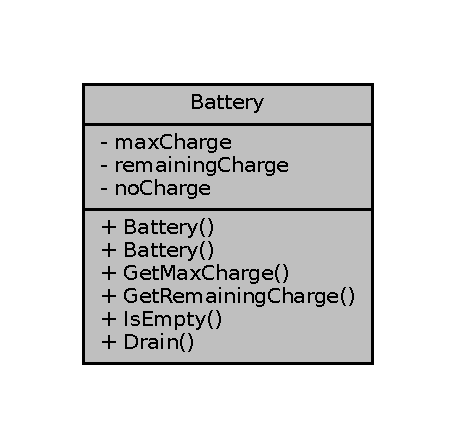
\includegraphics[width=219pt]{classBattery__coll__graph}
\end{center}
\end{figure}
\subsection*{Public Member Functions}
\begin{DoxyCompactItemize}
\item 
\mbox{\Hypertarget{classBattery_a36a6234c583e3b3506f4a77e3eb49989}\label{classBattery_a36a6234c583e3b3506f4a77e3eb49989}} 
\hyperlink{classBattery_a36a6234c583e3b3506f4a77e3eb49989}{Battery} ()
\begin{DoxyCompactList}\small\item\em default constructor \end{DoxyCompactList}\item 
\mbox{\Hypertarget{classBattery_a06a6a638724aeb3a1e45854a5e0e0b1c}\label{classBattery_a06a6a638724aeb3a1e45854a5e0e0b1c}} 
\hyperlink{classBattery_a06a6a638724aeb3a1e45854a5e0e0b1c}{Battery} (double max, double remaining, bool is\+Empty)
\begin{DoxyCompactList}\small\item\em constructor that takes arguments \end{DoxyCompactList}\item 
\mbox{\Hypertarget{classBattery_a40f54aa571826d0109465539bbc304b9}\label{classBattery_a40f54aa571826d0109465539bbc304b9}} 
double \hyperlink{classBattery_a40f54aa571826d0109465539bbc304b9}{Get\+Max\+Charge} ()
\begin{DoxyCompactList}\small\item\em getter\+: returns battery\textquotesingle{}s capacity \end{DoxyCompactList}\item 
\mbox{\Hypertarget{classBattery_a4abbd8d0e5005b17bfb6ed4e0038641a}\label{classBattery_a4abbd8d0e5005b17bfb6ed4e0038641a}} 
double \hyperlink{classBattery_a4abbd8d0e5005b17bfb6ed4e0038641a}{Get\+Remaining\+Charge} ()
\begin{DoxyCompactList}\small\item\em getter\+: returns charge left on battery \end{DoxyCompactList}\item 
\mbox{\Hypertarget{classBattery_a2b7a3315b5e1ca9c74ee64acf0bb2168}\label{classBattery_a2b7a3315b5e1ca9c74ee64acf0bb2168}} 
bool \hyperlink{classBattery_a2b7a3315b5e1ca9c74ee64acf0bb2168}{Is\+Empty} ()
\begin{DoxyCompactList}\small\item\em acts as a getter of our no\+Charge member variable. Just returns true or false on whether or not the battery is depleted. \end{DoxyCompactList}\item 
\mbox{\Hypertarget{classBattery_af3e0488dbe063350f3ab9077487d1e12}\label{classBattery_af3e0488dbe063350f3ab9077487d1e12}} 
void \hyperlink{classBattery_af3e0488dbe063350f3ab9077487d1e12}{Drain} (double percentage)
\begin{DoxyCompactList}\small\item\em this method changes the actual battery level. This operation would usually be called by a drone in it\textquotesingle{}s update method. \end{DoxyCompactList}\end{DoxyCompactItemize}
\subsection*{Private Attributes}
\begin{DoxyCompactItemize}
\item 
\mbox{\Hypertarget{classBattery_aa467c83e0fd2ea2d57d98f9e2dc341db}\label{classBattery_aa467c83e0fd2ea2d57d98f9e2dc341db}} 
double \hyperlink{classBattery_aa467c83e0fd2ea2d57d98f9e2dc341db}{max\+Charge}
\begin{DoxyCompactList}\small\item\em float depicting max charge of battery \end{DoxyCompactList}\item 
\mbox{\Hypertarget{classBattery_a4d012fbe92b40862bab89ce0019b7c0a}\label{classBattery_a4d012fbe92b40862bab89ce0019b7c0a}} 
double \hyperlink{classBattery_a4d012fbe92b40862bab89ce0019b7c0a}{remaining\+Charge}
\begin{DoxyCompactList}\small\item\em float depicting remaining charge of battery \end{DoxyCompactList}\item 
\mbox{\Hypertarget{classBattery_ac008f63a4d81761cc72fbae7356d8ff7}\label{classBattery_ac008f63a4d81761cc72fbae7356d8ff7}} 
bool \hyperlink{classBattery_ac008f63a4d81761cc72fbae7356d8ff7}{no\+Charge}
\begin{DoxyCompactList}\small\item\em boolean telling us whether or not bettery is depleted \end{DoxyCompactList}\end{DoxyCompactItemize}


\subsection{Detailed Description}
battery class. \hyperlink{classDrone}{Drone} and \hyperlink{classRobot}{Robot} objects have batteries that deplete over time. This class is used to represent the life of our drone and robot movable entities. 

The documentation for this class was generated from the following file\+:\begin{DoxyCompactItemize}
\item 
/home/user/repo/project/simulation/include/\hyperlink{battery_8h}{battery.\+h}\end{DoxyCompactItemize}

\hypertarget{classBeelineMovement}{}\section{Beeline\+Movement Class Reference}
\label{classBeelineMovement}\index{Beeline\+Movement@{Beeline\+Movement}}


Beeline movement-\/ will move directly towards a robot given a vector3 position. Extends \hyperlink{classiMovementStrategy}{i\+Movement\+Strategy} so each function overwrites the parent.  




{\ttfamily \#include $<$beeline\+\_\+movement.\+h$>$}



Inheritance diagram for Beeline\+Movement\+:\nopagebreak
\begin{figure}[H]
\begin{center}
\leavevmode
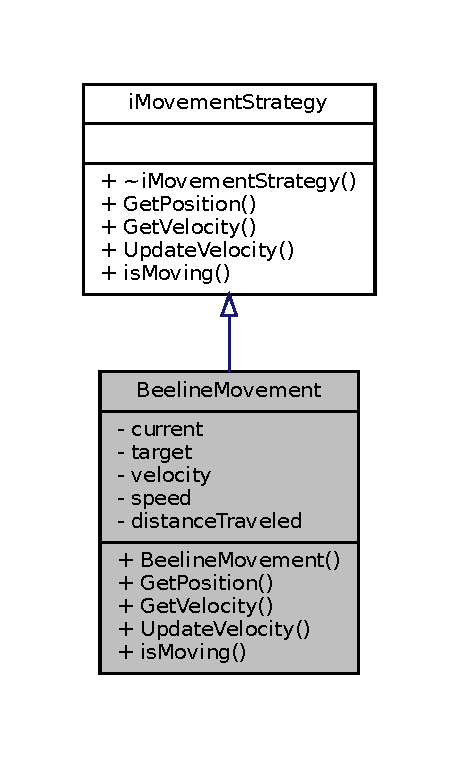
\includegraphics[width=220pt]{classBeelineMovement__inherit__graph}
\end{center}
\end{figure}


Collaboration diagram for Beeline\+Movement\+:\nopagebreak
\begin{figure}[H]
\begin{center}
\leavevmode
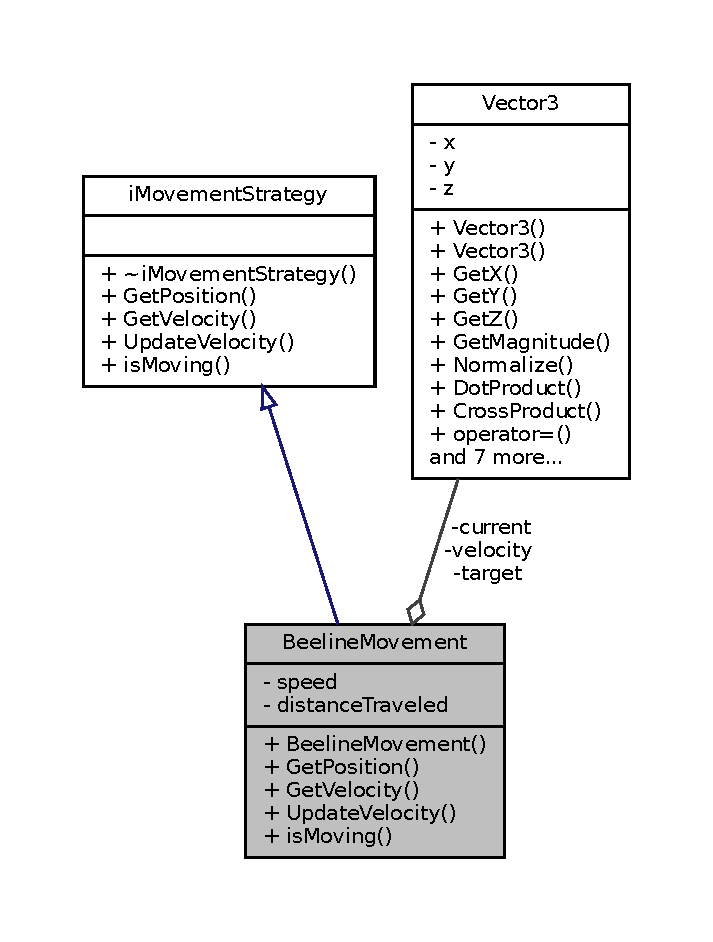
\includegraphics[width=342pt]{classBeelineMovement__coll__graph}
\end{center}
\end{figure}
\subsection*{Public Member Functions}
\begin{DoxyCompactItemize}
\item 
\mbox{\Hypertarget{classBeelineMovement_abebb0d5ff296ed7498b43438fffaddc3}\label{classBeelineMovement_abebb0d5ff296ed7498b43438fffaddc3}} 
\hyperlink{classBeelineMovement_abebb0d5ff296ed7498b43438fffaddc3}{Beeline\+Movement} (\hyperlink{classVector3}{Vector3} \hyperlink{classBeelineMovement_a78e1e59186f4e2082365c3d9816f96c5}{current}, \hyperlink{classVector3}{Vector3} \hyperlink{classBeelineMovement_a49239eec9d469db2fb34b4268a97da6e}{target}, double \hyperlink{classBeelineMovement_a580f1c87f104f067fb1ad09dbe3a83af}{speed})
\begin{DoxyCompactList}\small\item\em Constructor taking in \hyperlink{classVector3}{Vector3} objects for current position, target position, and a double speed at which the drone is traveling at. \end{DoxyCompactList}\item 
\hyperlink{classVector3}{Vector3} \hyperlink{classBeelineMovement_abfe070233bcdba668cd6f445b149f310}{Get\+Position} ()
\begin{DoxyCompactList}\small\item\em Current position getter. \end{DoxyCompactList}\item 
\hyperlink{classVector3}{Vector3} \hyperlink{classBeelineMovement_a20adc01dabe57edd17128b81ec49661a}{Get\+Velocity} ()
\begin{DoxyCompactList}\small\item\em Current velocity getter. \end{DoxyCompactList}\item 
\hyperlink{classVector3}{Vector3} \hyperlink{classBeelineMovement_a6fd4a3d6f7be2cb6dfe623ce40fc55c4}{Update\+Velocity} (double dt, \hyperlink{classVector3}{Vector3} \hyperlink{classBeelineMovement_a78e1e59186f4e2082365c3d9816f96c5}{current}, \hyperlink{classVector3}{Vector3} \hyperlink{classBeelineMovement_a49239eec9d469db2fb34b4268a97da6e}{target}, double time)
\begin{DoxyCompactList}\small\item\em Function to update velocity, takes in a double for time and \hyperlink{classVector3}{Vector3} objects for current and target positions. \end{DoxyCompactList}\item 
\mbox{\Hypertarget{classBeelineMovement_a9f2f68a5122dd168827843801cb932db}\label{classBeelineMovement_a9f2f68a5122dd168827843801cb932db}} 
bool {\bfseries is\+Moving} ()
\end{DoxyCompactItemize}
\subsection*{Private Attributes}
\begin{DoxyCompactItemize}
\item 
\mbox{\Hypertarget{classBeelineMovement_a78e1e59186f4e2082365c3d9816f96c5}\label{classBeelineMovement_a78e1e59186f4e2082365c3d9816f96c5}} 
\hyperlink{classVector3}{Vector3} \hyperlink{classBeelineMovement_a78e1e59186f4e2082365c3d9816f96c5}{current}
\begin{DoxyCompactList}\small\item\em \hyperlink{classVector3}{Vector3} current-\/ current position. \end{DoxyCompactList}\item 
\mbox{\Hypertarget{classBeelineMovement_a49239eec9d469db2fb34b4268a97da6e}\label{classBeelineMovement_a49239eec9d469db2fb34b4268a97da6e}} 
\hyperlink{classVector3}{Vector3} \hyperlink{classBeelineMovement_a49239eec9d469db2fb34b4268a97da6e}{target}
\begin{DoxyCompactList}\small\item\em \hyperlink{classVector3}{Vector3} target-\/ target position. \end{DoxyCompactList}\item 
\mbox{\Hypertarget{classBeelineMovement_a5fe0d89a9bad2fa05e662080accf924b}\label{classBeelineMovement_a5fe0d89a9bad2fa05e662080accf924b}} 
\hyperlink{classVector3}{Vector3} \hyperlink{classBeelineMovement_a5fe0d89a9bad2fa05e662080accf924b}{velocity}
\begin{DoxyCompactList}\small\item\em \hyperlink{classVector3}{Vector3} velocity-\/ current velocity. \end{DoxyCompactList}\item 
\mbox{\Hypertarget{classBeelineMovement_a580f1c87f104f067fb1ad09dbe3a83af}\label{classBeelineMovement_a580f1c87f104f067fb1ad09dbe3a83af}} 
double \hyperlink{classBeelineMovement_a580f1c87f104f067fb1ad09dbe3a83af}{speed}
\begin{DoxyCompactList}\small\item\em double speed-\/ current speed \end{DoxyCompactList}\item 
\mbox{\Hypertarget{classBeelineMovement_ad28d0dbbe30c429d3dd2b78c6c5c6a0f}\label{classBeelineMovement_ad28d0dbbe30c429d3dd2b78c6c5c6a0f}} 
double \hyperlink{classBeelineMovement_ad28d0dbbe30c429d3dd2b78c6c5c6a0f}{distance\+Traveled}
\begin{DoxyCompactList}\small\item\em double distance\+Traveled-\/ distace traveled using beeline \end{DoxyCompactList}\end{DoxyCompactItemize}


\subsection{Detailed Description}
Beeline movement-\/ will move directly towards a robot given a vector3 position. Extends \hyperlink{classiMovementStrategy}{i\+Movement\+Strategy} so each function overwrites the parent. 

\subsection{Member Function Documentation}
\mbox{\Hypertarget{classBeelineMovement_abfe070233bcdba668cd6f445b149f310}\label{classBeelineMovement_abfe070233bcdba668cd6f445b149f310}} 
\index{Beeline\+Movement@{Beeline\+Movement}!Get\+Position@{Get\+Position}}
\index{Get\+Position@{Get\+Position}!Beeline\+Movement@{Beeline\+Movement}}
\subsubsection{\texorpdfstring{Get\+Position()}{GetPosition()}}
{\footnotesize\ttfamily \hyperlink{classVector3}{Vector3} Beeline\+Movement\+::\+Get\+Position (\begin{DoxyParamCaption}{ }\end{DoxyParamCaption})\hspace{0.3cm}{\ttfamily [virtual]}}



Current position getter. 

\begin{DoxyReturn}{Returns}
\hyperlink{classVector3}{Vector3} position 
\end{DoxyReturn}


Implements \hyperlink{classiMovementStrategy_aa9f5a07461c654a7497775696d20e990}{i\+Movement\+Strategy}.

\mbox{\Hypertarget{classBeelineMovement_a20adc01dabe57edd17128b81ec49661a}\label{classBeelineMovement_a20adc01dabe57edd17128b81ec49661a}} 
\index{Beeline\+Movement@{Beeline\+Movement}!Get\+Velocity@{Get\+Velocity}}
\index{Get\+Velocity@{Get\+Velocity}!Beeline\+Movement@{Beeline\+Movement}}
\subsubsection{\texorpdfstring{Get\+Velocity()}{GetVelocity()}}
{\footnotesize\ttfamily \hyperlink{classVector3}{Vector3} Beeline\+Movement\+::\+Get\+Velocity (\begin{DoxyParamCaption}{ }\end{DoxyParamCaption})\hspace{0.3cm}{\ttfamily [virtual]}}



Current velocity getter. 

\begin{DoxyReturn}{Returns}
\hyperlink{classVector3}{Vector3} velocity 
\end{DoxyReturn}


Implements \hyperlink{classiMovementStrategy_a92f20c8ebf7c4f7dde5743528b8e45b7}{i\+Movement\+Strategy}.

\mbox{\Hypertarget{classBeelineMovement_a6fd4a3d6f7be2cb6dfe623ce40fc55c4}\label{classBeelineMovement_a6fd4a3d6f7be2cb6dfe623ce40fc55c4}} 
\index{Beeline\+Movement@{Beeline\+Movement}!Update\+Velocity@{Update\+Velocity}}
\index{Update\+Velocity@{Update\+Velocity}!Beeline\+Movement@{Beeline\+Movement}}
\subsubsection{\texorpdfstring{Update\+Velocity()}{UpdateVelocity()}}
{\footnotesize\ttfamily \hyperlink{classVector3}{Vector3} Beeline\+Movement\+::\+Update\+Velocity (\begin{DoxyParamCaption}\item[{double}]{dt,  }\item[{\hyperlink{classVector3}{Vector3}}]{current,  }\item[{\hyperlink{classVector3}{Vector3}}]{target,  }\item[{double}]{time }\end{DoxyParamCaption})\hspace{0.3cm}{\ttfamily [virtual]}}



Function to update velocity, takes in a double for time and \hyperlink{classVector3}{Vector3} objects for current and target positions. 

\begin{DoxyReturn}{Returns}
\hyperlink{classVector3}{Vector3} velocity 
\end{DoxyReturn}


Implements \hyperlink{classiMovementStrategy_a40ec6c329ca0842638af80cfd509b372}{i\+Movement\+Strategy}.



The documentation for this class was generated from the following files\+:\begin{DoxyCompactItemize}
\item 
/home/user/repo/project/simulation/include/\hyperlink{beeline__movement_8h}{beeline\+\_\+movement.\+h}\item 
/home/user/repo/project/simulation/src/beeline\+\_\+movement.\+cc\end{DoxyCompactItemize}

\hypertarget{classBlobDetectorAdapater}{}\section{Blob\+Detector\+Adapater Class Reference}
\label{classBlobDetectorAdapater}\index{Blob\+Detector\+Adapater@{Blob\+Detector\+Adapater}}


The Blob\+Detector\+Adapter class that interfaces the \hyperlink{classFilter}{Filter} and Open\+CV. This class scans an image for the orange drone using contours and morphing. If found, the drone data is stored in the pixel in the top left corner.  




{\ttfamily \#include $<$blob\+\_\+detector\+\_\+adapter.\+h$>$}



Inheritance diagram for Blob\+Detector\+Adapater\+:\nopagebreak
\begin{figure}[H]
\begin{center}
\leavevmode
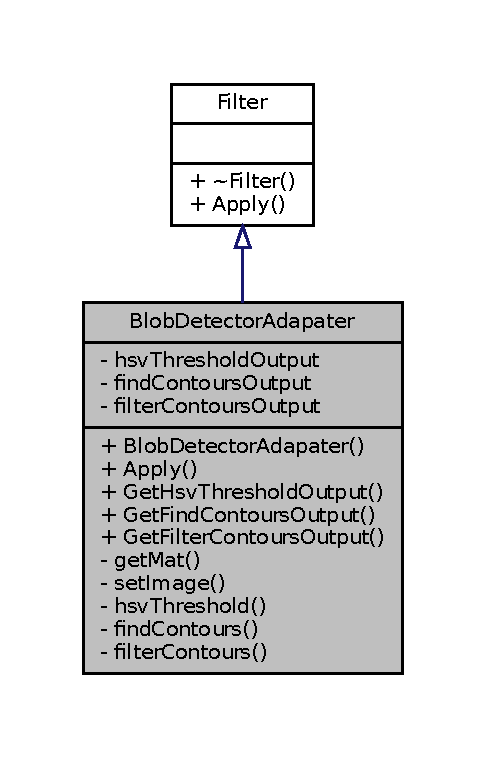
\includegraphics[width=233pt]{classBlobDetectorAdapater__inherit__graph}
\end{center}
\end{figure}


Collaboration diagram for Blob\+Detector\+Adapater\+:\nopagebreak
\begin{figure}[H]
\begin{center}
\leavevmode
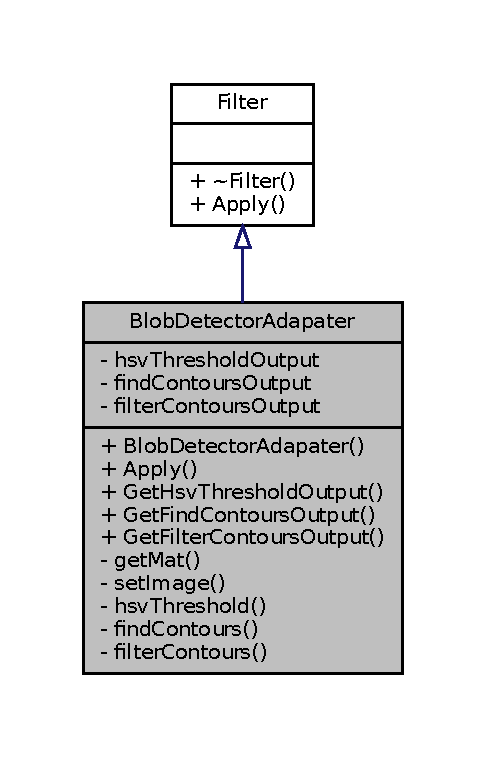
\includegraphics[width=233pt]{classBlobDetectorAdapater__coll__graph}
\end{center}
\end{figure}
\subsection*{Public Member Functions}
\begin{DoxyCompactItemize}
\item 
\mbox{\Hypertarget{classBlobDetectorAdapater_a971b9d9cbbfb9bafed2d5401e344264d}\label{classBlobDetectorAdapater_a971b9d9cbbfb9bafed2d5401e344264d}} 
\hyperlink{classBlobDetectorAdapater_a971b9d9cbbfb9bafed2d5401e344264d}{Blob\+Detector\+Adapater} ()
\begin{DoxyCompactList}\small\item\em Construct a new Blob Detector Adapater object. \end{DoxyCompactList}\item 
void \hyperlink{classBlobDetectorAdapater_a24f99498567e7b20b58a62aba78a759c}{Apply} (std\+::vector$<$ \hyperlink{classImage}{Image} $\ast$$>$ original, std\+::vector$<$ \hyperlink{classImage}{Image} $\ast$$>$ filtered)
\begin{DoxyCompactList}\small\item\em The overwritten apply function from \hyperlink{classFilter}{Filter}. Converts the original imges to cv\+::\+Mat and then runs Open\+CV blob detection. \end{DoxyCompactList}\item 
cv\+::\+Mat $\ast$ \hyperlink{classBlobDetectorAdapater_ae6cd1a0e7c6fdb0cdacdeba7bf472398}{Get\+Hsv\+Threshold\+Output} ()
\begin{DoxyCompactList}\small\item\em This method is a generated getter for the output of a R\+G\+B\+\_\+\+Threshold. \end{DoxyCompactList}\item 
std\+::vector$<$ std\+::vector$<$ cv\+::\+Point $>$ $>$ $\ast$ \hyperlink{classBlobDetectorAdapater_a9e688d27a238071e9445c07ac69c4941}{Get\+Find\+Contours\+Output} ()
\begin{DoxyCompactList}\small\item\em This method is a generated getter for the output of a Find\+\_\+\+Contours. \end{DoxyCompactList}\item 
std\+::vector$<$ std\+::vector$<$ cv\+::\+Point $>$ $>$ $\ast$ \hyperlink{classBlobDetectorAdapater_a7271f0c7a2797336777651fd7079fda6}{Get\+Filter\+Contours\+Output} ()
\begin{DoxyCompactList}\small\item\em This method is a generated getter for the output of a Filter\+\_\+\+Contours. \end{DoxyCompactList}\end{DoxyCompactItemize}
\subsection*{Private Member Functions}
\begin{DoxyCompactItemize}
\item 
\mbox{\Hypertarget{classBlobDetectorAdapater_a8c71f0f6253daf534c338bba8e5aea85}\label{classBlobDetectorAdapater_a8c71f0f6253daf534c338bba8e5aea85}} 
cv\+::\+Mat {\bfseries get\+Mat} (\hyperlink{classImage}{Image} $\ast$image)
\item 
\mbox{\Hypertarget{classBlobDetectorAdapater_aa9742425b9a1b8492a16a2ea20d115f8}\label{classBlobDetectorAdapater_aa9742425b9a1b8492a16a2ea20d115f8}} 
void {\bfseries set\+Image} (cv\+::\+Mat mat, \hyperlink{classImage}{Image} $\ast$image)
\item 
void \hyperlink{classBlobDetectorAdapater_ad6089c689fcfb884fc32ca4e3676f6ec}{hsv\+Threshold} (cv\+::\+Mat \&, double\mbox{[}$\,$\mbox{]}, double\mbox{[}$\,$\mbox{]}, double\mbox{[}$\,$\mbox{]}, cv\+::\+Mat \&)
\begin{DoxyCompactList}\small\item\em Segment an image based on color ranges. \end{DoxyCompactList}\item 
void \hyperlink{classBlobDetectorAdapater_aef56ed7c89479ff1a5b771e48738ce21}{find\+Contours} (cv\+::\+Mat \&, bool, std\+::vector$<$ std\+::vector$<$ cv\+::\+Point $>$$>$ \&)
\begin{DoxyCompactList}\small\item\em Finds contours in an image. \end{DoxyCompactList}\item 
void \hyperlink{classBlobDetectorAdapater_a5a627a8ae0ac83881e70ee096c69bdbd}{filter\+Contours} (cv\+::\+Mat \&, std\+::vector$<$ std\+::vector$<$ cv\+::\+Point $>$$>$ \&, double, double, double, double, double, double, double\mbox{[}$\,$\mbox{]}, double, double, double, double, std\+::vector$<$ std\+::vector$<$ cv\+::\+Point $>$$>$ \&)
\begin{DoxyCompactList}\small\item\em Filters through contours. \end{DoxyCompactList}\end{DoxyCompactItemize}
\subsection*{Private Attributes}
\begin{DoxyCompactItemize}
\item 
\mbox{\Hypertarget{classBlobDetectorAdapater_a544feb9ee51956c0569a24b59a2b737d}\label{classBlobDetectorAdapater_a544feb9ee51956c0569a24b59a2b737d}} 
cv\+::\+Mat {\bfseries hsv\+Threshold\+Output}
\item 
\mbox{\Hypertarget{classBlobDetectorAdapater_a4b59201e9c38c68bf833cc27ec9747dd}\label{classBlobDetectorAdapater_a4b59201e9c38c68bf833cc27ec9747dd}} 
std\+::vector$<$ std\+::vector$<$ cv\+::\+Point $>$ $>$ {\bfseries find\+Contours\+Output}
\item 
\mbox{\Hypertarget{classBlobDetectorAdapater_ad8418b4a8984b5db6fab8c8e7bd3ddbb}\label{classBlobDetectorAdapater_ad8418b4a8984b5db6fab8c8e7bd3ddbb}} 
std\+::vector$<$ std\+::vector$<$ cv\+::\+Point $>$ $>$ {\bfseries filter\+Contours\+Output}
\end{DoxyCompactItemize}


\subsection{Detailed Description}
The Blob\+Detector\+Adapter class that interfaces the \hyperlink{classFilter}{Filter} and Open\+CV. This class scans an image for the orange drone using contours and morphing. If found, the drone data is stored in the pixel in the top left corner. 

\subsection{Member Function Documentation}
\mbox{\Hypertarget{classBlobDetectorAdapater_a24f99498567e7b20b58a62aba78a759c}\label{classBlobDetectorAdapater_a24f99498567e7b20b58a62aba78a759c}} 
\index{Blob\+Detector\+Adapater@{Blob\+Detector\+Adapater}!Apply@{Apply}}
\index{Apply@{Apply}!Blob\+Detector\+Adapater@{Blob\+Detector\+Adapater}}
\subsubsection{\texorpdfstring{Apply()}{Apply()}}
{\footnotesize\ttfamily void Blob\+Detector\+Adapater\+::\+Apply (\begin{DoxyParamCaption}\item[{std\+::vector$<$ \hyperlink{classImage}{Image} $\ast$$>$}]{original,  }\item[{std\+::vector$<$ \hyperlink{classImage}{Image} $\ast$$>$}]{filtered }\end{DoxyParamCaption})\hspace{0.3cm}{\ttfamily [virtual]}}



The overwritten apply function from \hyperlink{classFilter}{Filter}. Converts the original imges to cv\+::\+Mat and then runs Open\+CV blob detection. 


\begin{DoxyParams}{Parameters}
{\em original} & \\
\hline
{\em filtered} & \\
\hline
\end{DoxyParams}
The following code was generated using the G\+R\+IP pipeline generator. This generator easily creates Open\+CV pipeline code to quickley view what the output of an Open\+CV pipeline will be. More information on G\+R\+IP\+: \href{https://github.com/WPIRoboticsProjects/GRIP/releases/tag/v1.5.2}{\tt https\+://github.\+com/\+W\+P\+I\+Robotics\+Projects/\+G\+R\+I\+P/releases/tag/v1.\+5.\+2}

This is the end of the G\+R\+IP generatored code

Implements \hyperlink{classFilter_afab0d50af44a19a370ebe46c69b8ff4e}{Filter}.

\mbox{\Hypertarget{classBlobDetectorAdapater_a5a627a8ae0ac83881e70ee096c69bdbd}\label{classBlobDetectorAdapater_a5a627a8ae0ac83881e70ee096c69bdbd}} 
\index{Blob\+Detector\+Adapater@{Blob\+Detector\+Adapater}!filter\+Contours@{filter\+Contours}}
\index{filter\+Contours@{filter\+Contours}!Blob\+Detector\+Adapater@{Blob\+Detector\+Adapater}}
\subsubsection{\texorpdfstring{filter\+Contours()}{filterContours()}}
{\footnotesize\ttfamily void Blob\+Detector\+Adapater\+::filter\+Contours (\begin{DoxyParamCaption}\item[{cv\+::\+Mat \&}]{,  }\item[{std\+::vector$<$ std\+::vector$<$ cv\+::\+Point $>$$>$ \&}]{,  }\item[{double}]{,  }\item[{double}]{,  }\item[{double}]{,  }\item[{double}]{,  }\item[{double}]{,  }\item[{double}]{,  }\item[{double}]{\mbox{[}$\,$\mbox{]},  }\item[{double}]{,  }\item[{double}]{,  }\item[{double}]{,  }\item[{double}]{,  }\item[{std\+::vector$<$ std\+::vector$<$ cv\+::\+Point $>$$>$ \&}]{ }\end{DoxyParamCaption})\hspace{0.3cm}{\ttfamily [private]}}



Filters through contours. 


\begin{DoxyParams}{Parameters}
{\em input\+Contours} & is the input vector of contours. \\
\hline
{\em min\+Area} & is the minimum area of a contour that will be kept. \\
\hline
{\em min\+Perimeter} & is the minimum perimeter of a contour that will be kept. \\
\hline
{\em min\+Width} & minimum width of a contour. \\
\hline
{\em max\+Width} & maximum width. \\
\hline
{\em min\+Height} & minimum height. \\
\hline
{\em max\+Height} & maximum height. \\
\hline
{\em solidity} & the minimum and maximum solidity of a contour. \\
\hline
{\em min\+Vertex\+Count} & minimum vertex Count of the contours. \\
\hline
{\em max\+Vertex\+Count} & maximum vertex Count. \\
\hline
{\em min\+Ratio} & minimum ratio of width to height. \\
\hline
{\em max\+Ratio} & maximum ratio of width to height. \\
\hline
{\em output} & vector of filtered contours. \\
\hline
\end{DoxyParams}
\mbox{\Hypertarget{classBlobDetectorAdapater_aef56ed7c89479ff1a5b771e48738ce21}\label{classBlobDetectorAdapater_aef56ed7c89479ff1a5b771e48738ce21}} 
\index{Blob\+Detector\+Adapater@{Blob\+Detector\+Adapater}!find\+Contours@{find\+Contours}}
\index{find\+Contours@{find\+Contours}!Blob\+Detector\+Adapater@{Blob\+Detector\+Adapater}}
\subsubsection{\texorpdfstring{find\+Contours()}{findContours()}}
{\footnotesize\ttfamily void Blob\+Detector\+Adapater\+::find\+Contours (\begin{DoxyParamCaption}\item[{cv\+::\+Mat \&}]{,  }\item[{bool}]{,  }\item[{std\+::vector$<$ std\+::vector$<$ cv\+::\+Point $>$$>$ \&}]{ }\end{DoxyParamCaption})\hspace{0.3cm}{\ttfamily [private]}}



Finds contours in an image. 


\begin{DoxyParams}{Parameters}
{\em input} & The image to find contours in. \\
\hline
{\em external\+Only} & if only external contours are to be found. \\
\hline
{\em contours} & vector of contours to put contours in. \\
\hline
\end{DoxyParams}
\mbox{\Hypertarget{classBlobDetectorAdapater_a7271f0c7a2797336777651fd7079fda6}\label{classBlobDetectorAdapater_a7271f0c7a2797336777651fd7079fda6}} 
\index{Blob\+Detector\+Adapater@{Blob\+Detector\+Adapater}!Get\+Filter\+Contours\+Output@{Get\+Filter\+Contours\+Output}}
\index{Get\+Filter\+Contours\+Output@{Get\+Filter\+Contours\+Output}!Blob\+Detector\+Adapater@{Blob\+Detector\+Adapater}}
\subsubsection{\texorpdfstring{Get\+Filter\+Contours\+Output()}{GetFilterContoursOutput()}}
{\footnotesize\ttfamily std\+::vector$<$ std\+::vector$<$ cv\+::\+Point $>$ $>$ $\ast$ Blob\+Detector\+Adapater\+::\+Get\+Filter\+Contours\+Output (\begin{DoxyParamCaption}{ }\end{DoxyParamCaption})}



This method is a generated getter for the output of a Filter\+\_\+\+Contours. 

\begin{DoxyReturn}{Returns}
Contours\+Report output from Filter\+\_\+\+Contours. 
\end{DoxyReturn}
\mbox{\Hypertarget{classBlobDetectorAdapater_a9e688d27a238071e9445c07ac69c4941}\label{classBlobDetectorAdapater_a9e688d27a238071e9445c07ac69c4941}} 
\index{Blob\+Detector\+Adapater@{Blob\+Detector\+Adapater}!Get\+Find\+Contours\+Output@{Get\+Find\+Contours\+Output}}
\index{Get\+Find\+Contours\+Output@{Get\+Find\+Contours\+Output}!Blob\+Detector\+Adapater@{Blob\+Detector\+Adapater}}
\subsubsection{\texorpdfstring{Get\+Find\+Contours\+Output()}{GetFindContoursOutput()}}
{\footnotesize\ttfamily std\+::vector$<$ std\+::vector$<$ cv\+::\+Point $>$ $>$ $\ast$ Blob\+Detector\+Adapater\+::\+Get\+Find\+Contours\+Output (\begin{DoxyParamCaption}{ }\end{DoxyParamCaption})}



This method is a generated getter for the output of a Find\+\_\+\+Contours. 

\begin{DoxyReturn}{Returns}
Contours\+Report output from Find\+\_\+\+Contours. 
\end{DoxyReturn}
\mbox{\Hypertarget{classBlobDetectorAdapater_ae6cd1a0e7c6fdb0cdacdeba7bf472398}\label{classBlobDetectorAdapater_ae6cd1a0e7c6fdb0cdacdeba7bf472398}} 
\index{Blob\+Detector\+Adapater@{Blob\+Detector\+Adapater}!Get\+Hsv\+Threshold\+Output@{Get\+Hsv\+Threshold\+Output}}
\index{Get\+Hsv\+Threshold\+Output@{Get\+Hsv\+Threshold\+Output}!Blob\+Detector\+Adapater@{Blob\+Detector\+Adapater}}
\subsubsection{\texorpdfstring{Get\+Hsv\+Threshold\+Output()}{GetHsvThresholdOutput()}}
{\footnotesize\ttfamily cv\+::\+Mat $\ast$ Blob\+Detector\+Adapater\+::\+Get\+Hsv\+Threshold\+Output (\begin{DoxyParamCaption}{ }\end{DoxyParamCaption})}



This method is a generated getter for the output of a R\+G\+B\+\_\+\+Threshold. 

The following is G\+R\+IP generatored helper functions \begin{DoxyReturn}{Returns}
Mat output from R\+G\+B\+\_\+\+Threshold. 
\end{DoxyReturn}
\mbox{\Hypertarget{classBlobDetectorAdapater_ad6089c689fcfb884fc32ca4e3676f6ec}\label{classBlobDetectorAdapater_ad6089c689fcfb884fc32ca4e3676f6ec}} 
\index{Blob\+Detector\+Adapater@{Blob\+Detector\+Adapater}!hsv\+Threshold@{hsv\+Threshold}}
\index{hsv\+Threshold@{hsv\+Threshold}!Blob\+Detector\+Adapater@{Blob\+Detector\+Adapater}}
\subsubsection{\texorpdfstring{hsv\+Threshold()}{hsvThreshold()}}
{\footnotesize\ttfamily void Blob\+Detector\+Adapater\+::hsv\+Threshold (\begin{DoxyParamCaption}\item[{cv\+::\+Mat \&}]{input,  }\item[{double}]{hue\mbox{[}$\,$\mbox{]},  }\item[{double}]{saturation\mbox{[}$\,$\mbox{]},  }\item[{double}]{value\mbox{[}$\,$\mbox{]},  }\item[{cv\+::\+Mat \&}]{output }\end{DoxyParamCaption})\hspace{0.3cm}{\ttfamily [private]}}



Segment an image based on color ranges. 


\begin{DoxyParams}{Parameters}
{\em input} & The image on which to perform the R\+GB threshold. \\
\hline
{\em red} & The min and max red. \\
\hline
{\em green} & The min and max green. \\
\hline
{\em blue} & The min and max blue. \\
\hline
{\em output} & The image in which to store the output. \\
\hline
\end{DoxyParams}


The documentation for this class was generated from the following files\+:\begin{DoxyCompactItemize}
\item 
/home/user/repo/project/image/include/\hyperlink{blob__detector__adapter_8h}{blob\+\_\+detector\+\_\+adapter.\+h}\item 
/home/user/repo/project/image/src/blob\+\_\+detector\+\_\+adapter.\+cc\end{DoxyCompactItemize}

\hypertarget{classBreadthFirstSearch}{}\section{Breadth\+First\+Search Class Reference}
\label{classBreadthFirstSearch}\index{Breadth\+First\+Search@{Breadth\+First\+Search}}


Beeline movement-\/ will move directly towards a robot given a vector3 position. extends \hyperlink{classiMovementStrategy}{i\+Movement\+Strategy} so each function overwrites the parent.  




{\ttfamily \#include $<$breadth\+\_\+first\+\_\+search.\+h$>$}



Inheritance diagram for Breadth\+First\+Search\+:\nopagebreak
\begin{figure}[H]
\begin{center}
\leavevmode
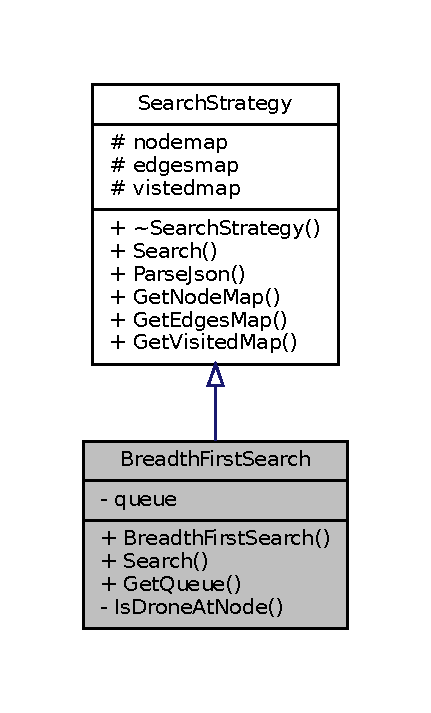
\includegraphics[width=207pt]{classBreadthFirstSearch__inherit__graph}
\end{center}
\end{figure}


Collaboration diagram for Breadth\+First\+Search\+:\nopagebreak
\begin{figure}[H]
\begin{center}
\leavevmode
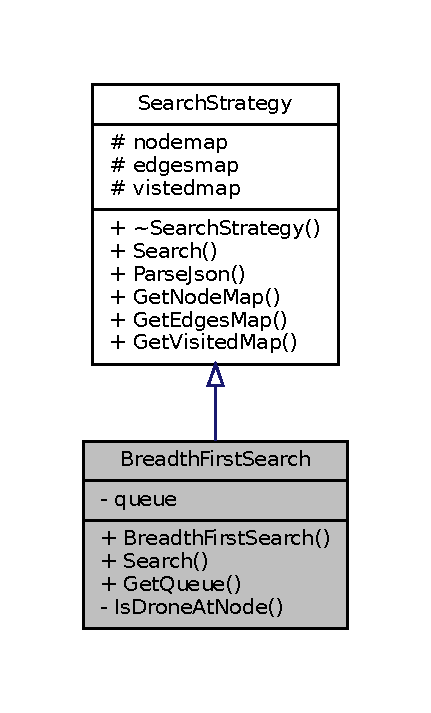
\includegraphics[width=207pt]{classBreadthFirstSearch__coll__graph}
\end{center}
\end{figure}
\subsection*{Public Member Functions}
\begin{DoxyCompactItemize}
\item 
\mbox{\Hypertarget{classBreadthFirstSearch_a5a9f84e4b10107e8e809349292f6ca76}\label{classBreadthFirstSearch_a5a9f84e4b10107e8e809349292f6ca76}} 
\hyperlink{classBreadthFirstSearch_a5a9f84e4b10107e8e809349292f6ca76}{Breadth\+First\+Search} ()
\begin{DoxyCompactList}\small\item\em default constructor \end{DoxyCompactList}\item 
\mbox{\Hypertarget{classBreadthFirstSearch_a69eb7594b796343b19d5f8d4a67516d3}\label{classBreadthFirstSearch_a69eb7594b796343b19d5f8d4a67516d3}} 
\hyperlink{classVector3}{Vector3} $\ast$ \hyperlink{classBreadthFirstSearch_a69eb7594b796343b19d5f8d4a67516d3}{Search} (\hyperlink{classVector3}{Vector3} current\+Pos)
\begin{DoxyCompactList}\small\item\em Searching function for Breadth First Search. \end{DoxyCompactList}\item 
\mbox{\Hypertarget{classBreadthFirstSearch_a73ddb06824da940bbb5f8da61cf58419}\label{classBreadthFirstSearch_a73ddb06824da940bbb5f8da61cf58419}} 
std\+::queue$<$ std\+::string $>$ \hyperlink{classBreadthFirstSearch_a73ddb06824da940bbb5f8da61cf58419}{Get\+Queue} ()
\begin{DoxyCompactList}\small\item\em Returns Queue. \end{DoxyCompactList}\end{DoxyCompactItemize}
\subsection*{Private Member Functions}
\begin{DoxyCompactItemize}
\item 
\mbox{\Hypertarget{classBreadthFirstSearch_a2f7227457d7b1e77a1345f38bfb16d36}\label{classBreadthFirstSearch_a2f7227457d7b1e77a1345f38bfb16d36}} 
bool \hyperlink{classBreadthFirstSearch_a2f7227457d7b1e77a1345f38bfb16d36}{Is\+Drone\+At\+Node} (\hyperlink{classVector3}{Vector3} current\+Pos)
\begin{DoxyCompactList}\small\item\em Private bool to see the the drone is currently at the expected node or not. \end{DoxyCompactList}\end{DoxyCompactItemize}
\subsection*{Private Attributes}
\begin{DoxyCompactItemize}
\item 
\mbox{\Hypertarget{classBreadthFirstSearch_a577ce5c2d8206b1b79f4de751960f3f4}\label{classBreadthFirstSearch_a577ce5c2d8206b1b79f4de751960f3f4}} 
std\+::queue$<$ std\+::string $>$ \hyperlink{classBreadthFirstSearch_a577ce5c2d8206b1b79f4de751960f3f4}{queue}
\begin{DoxyCompactList}\small\item\em Queue for \hyperlink{classBreadthFirstSearch}{Breadth\+First\+Search} searching. \end{DoxyCompactList}\end{DoxyCompactItemize}
\subsection*{Additional Inherited Members}


\subsection{Detailed Description}
Beeline movement-\/ will move directly towards a robot given a vector3 position. extends \hyperlink{classiMovementStrategy}{i\+Movement\+Strategy} so each function overwrites the parent. 

The documentation for this class was generated from the following files\+:\begin{DoxyCompactItemize}
\item 
/home/user/repo/project/simulation/include/\hyperlink{breadth__first__search_8h}{breadth\+\_\+first\+\_\+search.\+h}\item 
/home/user/repo/project/simulation/src/breadth\+\_\+first\+\_\+search.\+cc\end{DoxyCompactItemize}

\hypertarget{classCamera}{}\section{Camera Class Reference}
\label{classCamera}\index{Camera@{Camera}}


The camera class. This class can be attached to any entity and act as a camera. When attached to the web app observer, it can receive pictures from the simulation and process the contents of them and return Camera\+Results.  




{\ttfamily \#include $<$camera.\+h$>$}



Inheritance diagram for Camera\+:\nopagebreak
\begin{figure}[H]
\begin{center}
\leavevmode
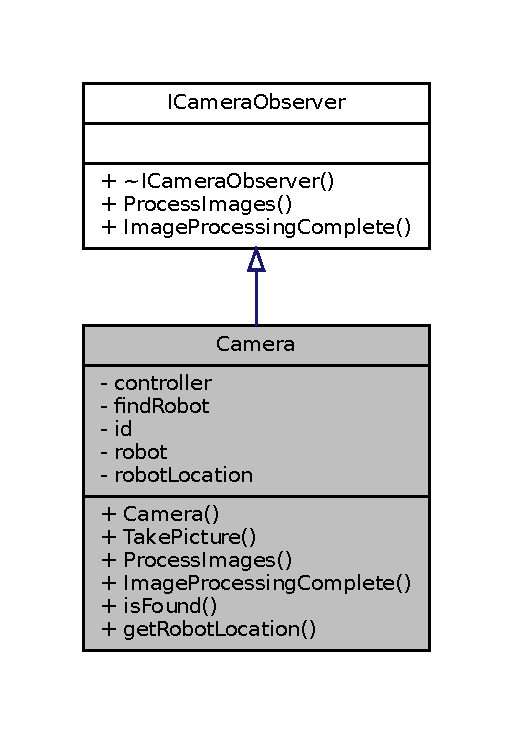
\includegraphics[width=246pt]{classCamera__inherit__graph}
\end{center}
\end{figure}


Collaboration diagram for Camera\+:\nopagebreak
\begin{figure}[H]
\begin{center}
\leavevmode
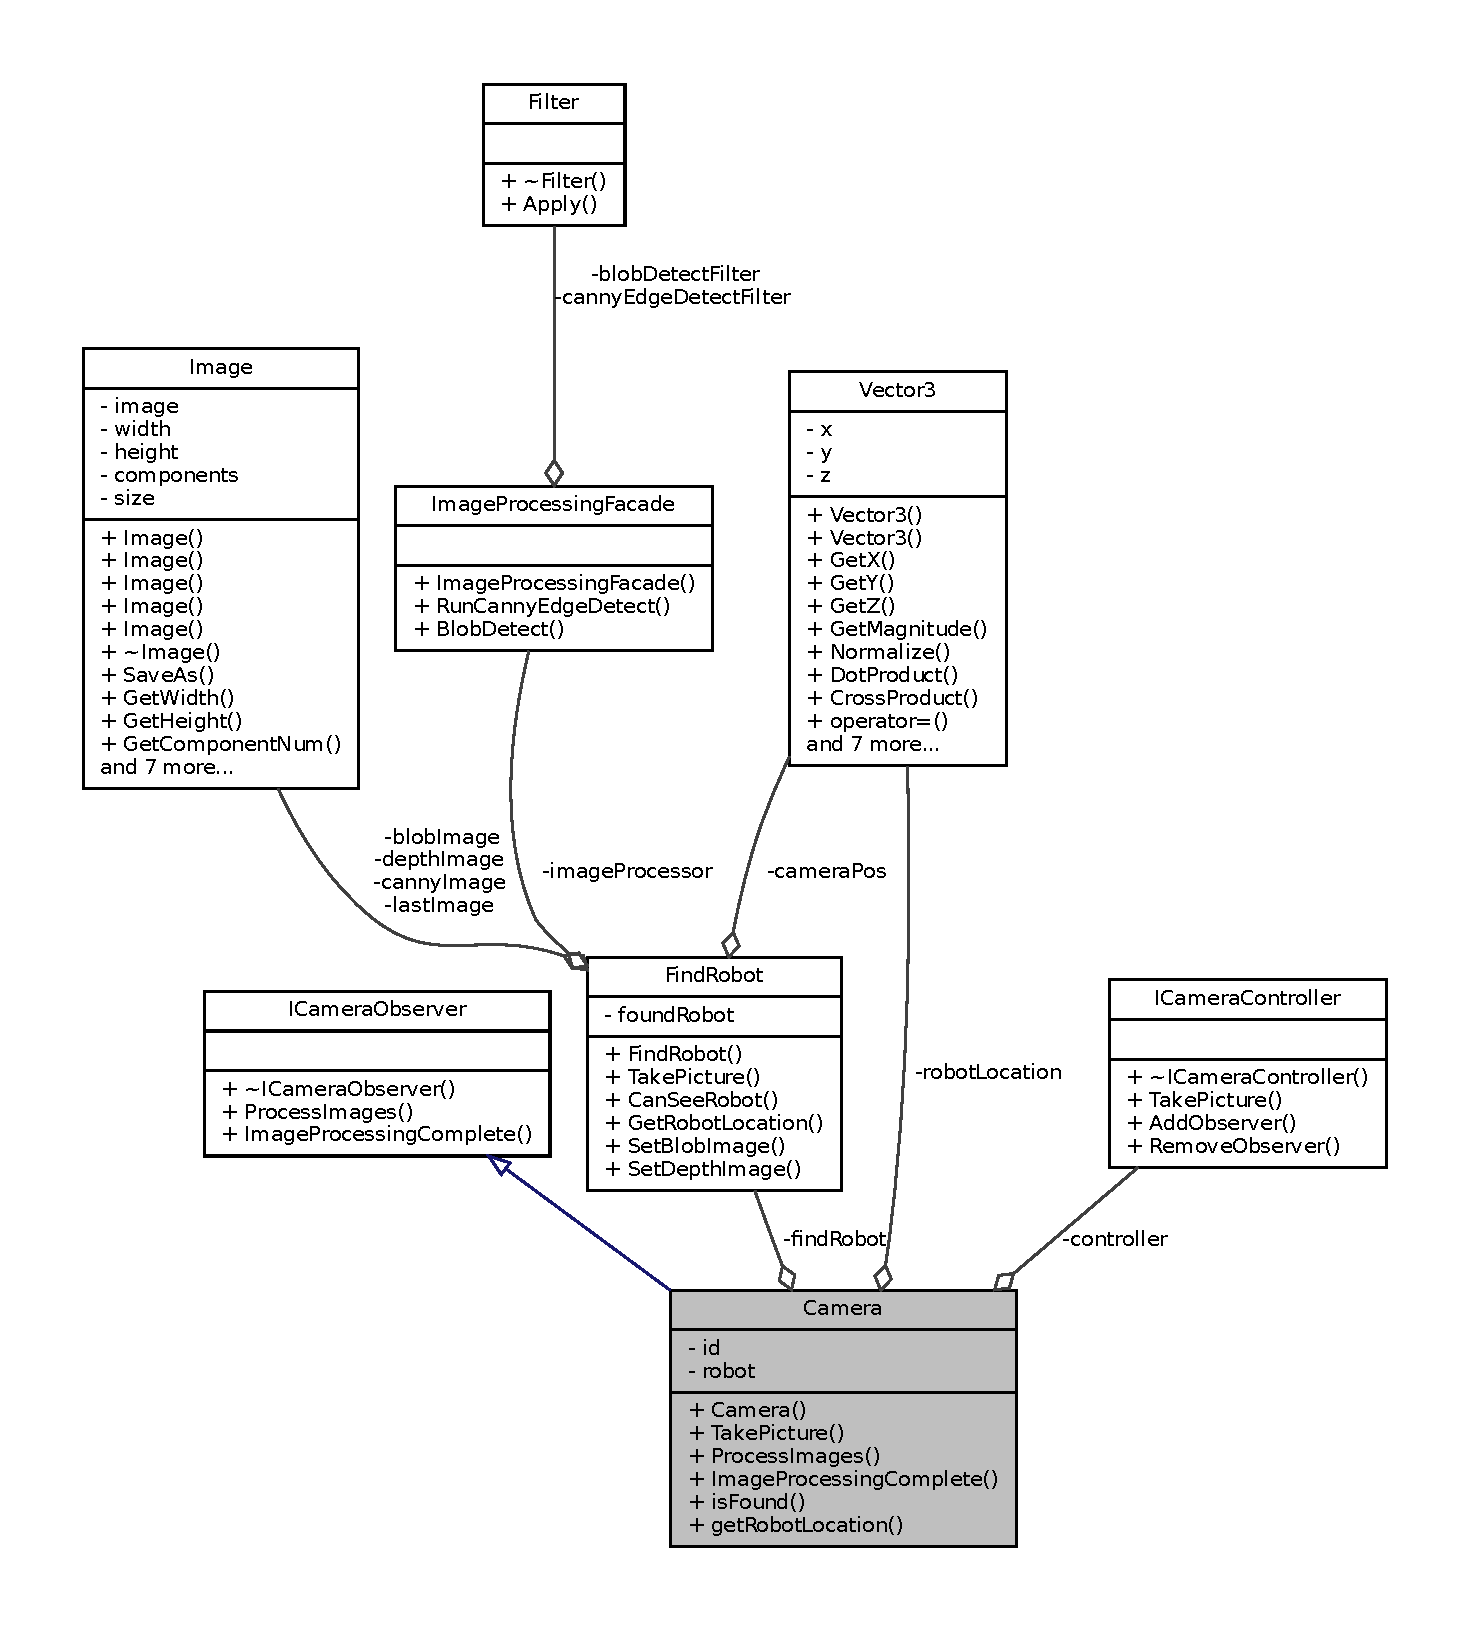
\includegraphics[width=350pt]{classCamera__coll__graph}
\end{center}
\end{figure}
\subsection*{Classes}
\begin{DoxyCompactItemize}
\item 
struct \hyperlink{structCamera_1_1CameraResult}{Camera\+Result}
\begin{DoxyCompactList}\small\item\em The struct that holds all the information for the camera results once, image processing is completed. \end{DoxyCompactList}\end{DoxyCompactItemize}
\subsection*{Public Member Functions}
\begin{DoxyCompactItemize}
\item 
\hyperlink{classCamera_a94c943c9dbc0d75340f34d3816eec8fc}{Camera} (int camera\+Id, \hyperlink{classICameraController}{I\+Camera\+Controller} $\ast$\hyperlink{classCamera_aca1a708bb6132877f6be0b62cfe2c834}{controller})
\begin{DoxyCompactList}\small\item\em Construct a new \hyperlink{classCamera}{Camera} object. Sets the observer, and initializes the find robot class. \end{DoxyCompactList}\item 
\mbox{\Hypertarget{classCamera_a70dfc7f06d6e12855afadd358831cf3a}\label{classCamera_a70dfc7f06d6e12855afadd358831cf3a}} 
void \hyperlink{classCamera_a70dfc7f06d6e12855afadd358831cf3a}{Take\+Picture} ()
\begin{DoxyCompactList}\small\item\em This is the function that tell the simulation that this camera would like a new picture for image processing. \end{DoxyCompactList}\item 
\hyperlink{classICameraResult}{I\+Camera\+Result} $\ast$ \hyperlink{classCamera_a792611ad34a1c595b61b7c72ce1d5e32}{Process\+Images} (int camera\+Id, double x\+Pos, double y\+Pos, double z\+Pos, const std\+::vector$<$ \hyperlink{structRawCameraImage}{Raw\+Camera\+Image} $>$ \&images, picojson\+::object \&details) const
\begin{DoxyCompactList}\small\item\em After the simulation takes a photo, it adds to a thread safe queue that this function reads from and can run image processing functionality on the given image. \end{DoxyCompactList}\item 
void \hyperlink{classCamera_a28c3836707bdaf6e1a2098ec20460995}{Image\+Processing\+Complete} (\hyperlink{classICameraResult}{I\+Camera\+Result} $\ast$result)
\begin{DoxyCompactList}\small\item\em This allows other threads to view the results of the last processed image. \end{DoxyCompactList}\item 
bool \hyperlink{classCamera_a7a88bbfa9d8529f4351f5a7396d5e80b}{is\+Found} ()
\begin{DoxyCompactList}\small\item\em Returns if the camera sees the robot. \end{DoxyCompactList}\item 
\hyperlink{classVector3}{Vector3} \hyperlink{classCamera_a23e1dc349268eafe666b83d0a3b831a2}{get\+Robot\+Location} ()
\begin{DoxyCompactList}\small\item\em Get the \hyperlink{classRobot}{Robot} Location object. \end{DoxyCompactList}\end{DoxyCompactItemize}
\subsection*{Private Attributes}
\begin{DoxyCompactItemize}
\item 
\mbox{\Hypertarget{classCamera_aca1a708bb6132877f6be0b62cfe2c834}\label{classCamera_aca1a708bb6132877f6be0b62cfe2c834}} 
\hyperlink{classICameraController}{I\+Camera\+Controller} $\ast$ \hyperlink{classCamera_aca1a708bb6132877f6be0b62cfe2c834}{controller}
\begin{DoxyCompactList}\small\item\em The camera controller that takes photos, usually the web app. \end{DoxyCompactList}\item 
\mbox{\Hypertarget{classCamera_a525dfb163566c33bcbf439714bc4f352}\label{classCamera_a525dfb163566c33bcbf439714bc4f352}} 
\hyperlink{classFindRobot}{Find\+Robot} $\ast$ \hyperlink{classCamera_a525dfb163566c33bcbf439714bc4f352}{find\+Robot}
\begin{DoxyCompactList}\small\item\em The find robot class that can actually run image processing on the images. \end{DoxyCompactList}\item 
\mbox{\Hypertarget{classCamera_a4777e12d1a1138468a2d9023d8bff4ec}\label{classCamera_a4777e12d1a1138468a2d9023d8bff4ec}} 
int \hyperlink{classCamera_a4777e12d1a1138468a2d9023d8bff4ec}{id}
\begin{DoxyCompactList}\small\item\em The id of the camera, corresponds to the id of the entity it\textquotesingle{}s attached to. \end{DoxyCompactList}\item 
\mbox{\Hypertarget{classCamera_a80a8ae81e244769c5d5c36c6c994a04b}\label{classCamera_a80a8ae81e244769c5d5c36c6c994a04b}} 
bool \hyperlink{classCamera_a80a8ae81e244769c5d5c36c6c994a04b}{robot}
\begin{DoxyCompactList}\small\item\em Has the camera seen the robot yet. \end{DoxyCompactList}\item 
\mbox{\Hypertarget{classCamera_a38e395108a9ba7b0e0ce2d1110ec70d9}\label{classCamera_a38e395108a9ba7b0e0ce2d1110ec70d9}} 
\hyperlink{classVector3}{Vector3} \hyperlink{classCamera_a38e395108a9ba7b0e0ce2d1110ec70d9}{robot\+Location}
\begin{DoxyCompactList}\small\item\em Gets the robot location. \end{DoxyCompactList}\end{DoxyCompactItemize}


\subsection{Detailed Description}
The camera class. This class can be attached to any entity and act as a camera. When attached to the web app observer, it can receive pictures from the simulation and process the contents of them and return Camera\+Results. 

\subsection{Constructor \& Destructor Documentation}
\mbox{\Hypertarget{classCamera_a94c943c9dbc0d75340f34d3816eec8fc}\label{classCamera_a94c943c9dbc0d75340f34d3816eec8fc}} 
\index{Camera@{Camera}!Camera@{Camera}}
\index{Camera@{Camera}!Camera@{Camera}}
\subsubsection{\texorpdfstring{Camera()}{Camera()}}
{\footnotesize\ttfamily Camera\+::\+Camera (\begin{DoxyParamCaption}\item[{int}]{camera\+Id,  }\item[{\hyperlink{classICameraController}{I\+Camera\+Controller} $\ast$}]{controller }\end{DoxyParamCaption})\hspace{0.3cm}{\ttfamily [inline]}}



Construct a new \hyperlink{classCamera}{Camera} object. Sets the observer, and initializes the find robot class. 


\begin{DoxyParams}{Parameters}
{\em camera\+Id} & \\
\hline
{\em controller} & \\
\hline
\end{DoxyParams}


\subsection{Member Function Documentation}
\mbox{\Hypertarget{classCamera_a23e1dc349268eafe666b83d0a3b831a2}\label{classCamera_a23e1dc349268eafe666b83d0a3b831a2}} 
\index{Camera@{Camera}!get\+Robot\+Location@{get\+Robot\+Location}}
\index{get\+Robot\+Location@{get\+Robot\+Location}!Camera@{Camera}}
\subsubsection{\texorpdfstring{get\+Robot\+Location()}{getRobotLocation()}}
{\footnotesize\ttfamily \hyperlink{classVector3}{Vector3} Camera\+::get\+Robot\+Location (\begin{DoxyParamCaption}{ }\end{DoxyParamCaption})}



Get the \hyperlink{classRobot}{Robot} Location object. 

\begin{DoxyReturn}{Returns}
\hyperlink{classVector3}{Vector3} 
\end{DoxyReturn}
\mbox{\Hypertarget{classCamera_a28c3836707bdaf6e1a2098ec20460995}\label{classCamera_a28c3836707bdaf6e1a2098ec20460995}} 
\index{Camera@{Camera}!Image\+Processing\+Complete@{Image\+Processing\+Complete}}
\index{Image\+Processing\+Complete@{Image\+Processing\+Complete}!Camera@{Camera}}
\subsubsection{\texorpdfstring{Image\+Processing\+Complete()}{ImageProcessingComplete()}}
{\footnotesize\ttfamily void Camera\+::\+Image\+Processing\+Complete (\begin{DoxyParamCaption}\item[{\hyperlink{classICameraResult}{I\+Camera\+Result} $\ast$}]{result }\end{DoxyParamCaption})\hspace{0.3cm}{\ttfamily [virtual]}}



This allows other threads to view the results of the last processed image. 


\begin{DoxyParams}{Parameters}
{\em result} & \\
\hline
\end{DoxyParams}


Implements \hyperlink{classICameraObserver_a7d261bd08d570d05032e61b2d5252c88}{I\+Camera\+Observer}.

\mbox{\Hypertarget{classCamera_a7a88bbfa9d8529f4351f5a7396d5e80b}\label{classCamera_a7a88bbfa9d8529f4351f5a7396d5e80b}} 
\index{Camera@{Camera}!is\+Found@{is\+Found}}
\index{is\+Found@{is\+Found}!Camera@{Camera}}
\subsubsection{\texorpdfstring{is\+Found()}{isFound()}}
{\footnotesize\ttfamily bool Camera\+::is\+Found (\begin{DoxyParamCaption}{ }\end{DoxyParamCaption})}



Returns if the camera sees the robot. 

\begin{DoxyReturn}{Returns}
true 

false 
\end{DoxyReturn}
\mbox{\Hypertarget{classCamera_a792611ad34a1c595b61b7c72ce1d5e32}\label{classCamera_a792611ad34a1c595b61b7c72ce1d5e32}} 
\index{Camera@{Camera}!Process\+Images@{Process\+Images}}
\index{Process\+Images@{Process\+Images}!Camera@{Camera}}
\subsubsection{\texorpdfstring{Process\+Images()}{ProcessImages()}}
{\footnotesize\ttfamily \hyperlink{classICameraResult}{I\+Camera\+Result} $\ast$ Camera\+::\+Process\+Images (\begin{DoxyParamCaption}\item[{int}]{camera\+Id,  }\item[{double}]{x\+Pos,  }\item[{double}]{y\+Pos,  }\item[{double}]{z\+Pos,  }\item[{const std\+::vector$<$ \hyperlink{structRawCameraImage}{Raw\+Camera\+Image} $>$ \&}]{images,  }\item[{picojson\+::object \&}]{details }\end{DoxyParamCaption}) const\hspace{0.3cm}{\ttfamily [virtual]}}



After the simulation takes a photo, it adds to a thread safe queue that this function reads from and can run image processing functionality on the given image. 


\begin{DoxyParams}{Parameters}
{\em camera\+Id} & \\
\hline
{\em x\+Pos} & \\
\hline
{\em y\+Pos} & \\
\hline
{\em z\+Pos} & \\
\hline
{\em images} & \\
\hline
{\em details} & \\
\hline
\end{DoxyParams}
\begin{DoxyReturn}{Returns}
I\+Camera\+Result$\ast$ 
\end{DoxyReturn}


Implements \hyperlink{classICameraObserver_aec871459f2c429b4334769021b72ec34}{I\+Camera\+Observer}.



The documentation for this class was generated from the following files\+:\begin{DoxyCompactItemize}
\item 
/home/user/repo/project/simulation/include/\hyperlink{camera_8h}{camera.\+h}\item 
/home/user/repo/project/simulation/src/camera.\+cc\end{DoxyCompactItemize}

\hypertarget{structCamera_1_1CameraResult}{}\section{Camera\+:\+:Camera\+Result Struct Reference}
\label{structCamera_1_1CameraResult}\index{Camera\+::\+Camera\+Result@{Camera\+::\+Camera\+Result}}


The struct that holds all the information for the camera results once, image processing is completed.  




{\ttfamily \#include $<$camera.\+h$>$}



Inheritance diagram for Camera\+:\+:Camera\+Result\+:\nopagebreak
\begin{figure}[H]
\begin{center}
\leavevmode
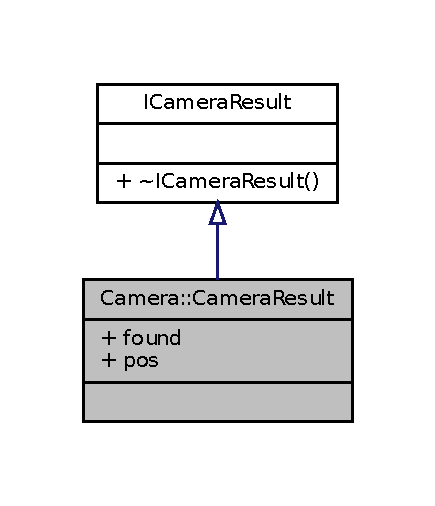
\includegraphics[width=209pt]{structCamera_1_1CameraResult__inherit__graph}
\end{center}
\end{figure}


Collaboration diagram for Camera\+:\+:Camera\+Result\+:\nopagebreak
\begin{figure}[H]
\begin{center}
\leavevmode
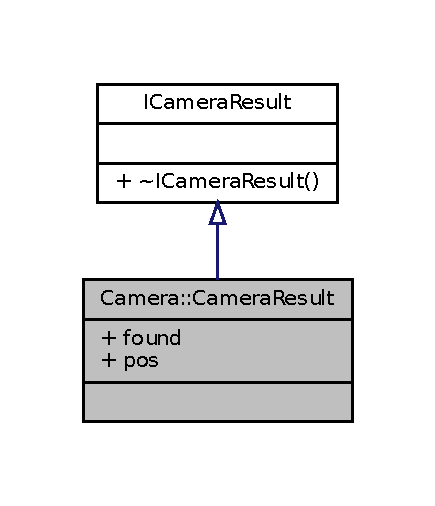
\includegraphics[width=209pt]{structCamera_1_1CameraResult__coll__graph}
\end{center}
\end{figure}
\subsection*{Public Attributes}
\begin{DoxyCompactItemize}
\item 
\mbox{\Hypertarget{structCamera_1_1CameraResult_acad6e14dede05ba7da513b5d0c8e146b}\label{structCamera_1_1CameraResult_acad6e14dede05ba7da513b5d0c8e146b}} 
bool {\bfseries found}
\item 
\mbox{\Hypertarget{structCamera_1_1CameraResult_aaa861cab42ce352258a46c49fba5a0d9}\label{structCamera_1_1CameraResult_aaa861cab42ce352258a46c49fba5a0d9}} 
double {\bfseries pos} \mbox{[}3\mbox{]}
\end{DoxyCompactItemize}
\subsection*{Additional Inherited Members}


\subsection{Detailed Description}
The struct that holds all the information for the camera results once, image processing is completed. 

The documentation for this struct was generated from the following file\+:\begin{DoxyCompactItemize}
\item 
/home/user/repo/project/simulation/include/\hyperlink{camera_8h}{camera.\+h}\end{DoxyCompactItemize}

\hypertarget{classCannyEdgeDetect}{}\section{Canny\+Edge\+Detect Class Reference}
\label{classCannyEdgeDetect}\index{Canny\+Edge\+Detect@{Canny\+Edge\+Detect}}


The main class for \hyperlink{classCannyEdgeDetect}{Canny\+Edge\+Detect}, extends \hyperlink{classFilter}{Filter}. This basically just applies each of the filters required for the canny edge algorthim in order,.  




{\ttfamily \#include $<$canny\+\_\+edge\+\_\+detect.\+h$>$}



Inheritance diagram for Canny\+Edge\+Detect\+:\nopagebreak
\begin{figure}[H]
\begin{center}
\leavevmode
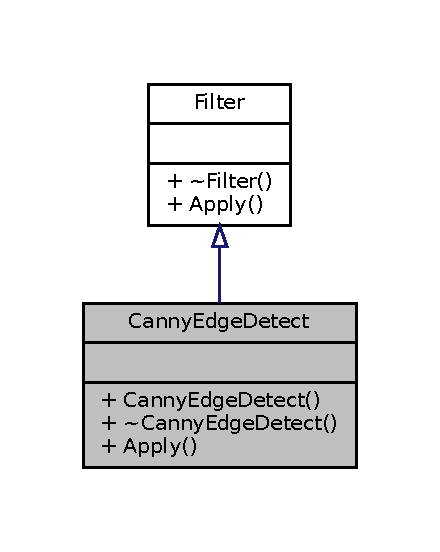
\includegraphics[width=211pt]{classCannyEdgeDetect__inherit__graph}
\end{center}
\end{figure}


Collaboration diagram for Canny\+Edge\+Detect\+:\nopagebreak
\begin{figure}[H]
\begin{center}
\leavevmode
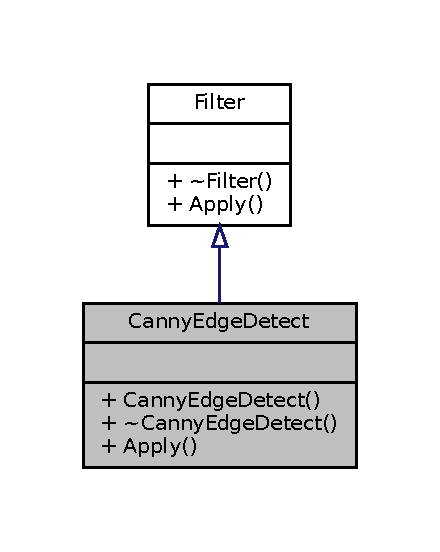
\includegraphics[width=211pt]{classCannyEdgeDetect__coll__graph}
\end{center}
\end{figure}
\subsection*{Public Member Functions}
\begin{DoxyCompactItemize}
\item 
\mbox{\Hypertarget{classCannyEdgeDetect_abe04677896a21d58d144783cc3aefb35}\label{classCannyEdgeDetect_abe04677896a21d58d144783cc3aefb35}} 
\hyperlink{classCannyEdgeDetect_abe04677896a21d58d144783cc3aefb35}{Canny\+Edge\+Detect} ()
\begin{DoxyCompactList}\small\item\em Constructor. \end{DoxyCompactList}\item 
\mbox{\Hypertarget{classCannyEdgeDetect_a4ccdf28f996d538eb8aee486acfbaea3}\label{classCannyEdgeDetect_a4ccdf28f996d538eb8aee486acfbaea3}} 
\hyperlink{classCannyEdgeDetect_a4ccdf28f996d538eb8aee486acfbaea3}{$\sim$\+Canny\+Edge\+Detect} ()
\begin{DoxyCompactList}\small\item\em Destructor. \end{DoxyCompactList}\item 
\mbox{\Hypertarget{classCannyEdgeDetect_a906422525db16b541c1765b431865e58}\label{classCannyEdgeDetect_a906422525db16b541c1765b431865e58}} 
void \hyperlink{classCannyEdgeDetect_a906422525db16b541c1765b431865e58}{Apply} (std\+::vector$<$ \hyperlink{classImage}{Image} $\ast$$>$ original, std\+::vector$<$ \hyperlink{classImage}{Image} $\ast$$>$ filtered)
\begin{DoxyCompactList}\small\item\em Apply function to be overridden by \hyperlink{classFilter}{Filter} Apply function. \end{DoxyCompactList}\end{DoxyCompactItemize}


\subsection{Detailed Description}
The main class for \hyperlink{classCannyEdgeDetect}{Canny\+Edge\+Detect}, extends \hyperlink{classFilter}{Filter}. This basically just applies each of the filters required for the canny edge algorthim in order,. 


\begin{DoxyEnumerate}
\item Greyscale
\item Gaussian Blur
\item Sobel
\item Non-\/\+Max Suppression
\item Double Threshold
\item Hysteresis To see more information on how this works\+: \href{https://towardsdatascience.com/canny-edge-detection-step-by-step-in-python-computer-vision-b49c3a2d8123}{\tt https\+://towardsdatascience.\+com/canny-\/edge-\/detection-\/step-\/by-\/step-\/in-\/python-\/computer-\/vision-\/b49c3a2d8123} 
\end{DoxyEnumerate}

The documentation for this class was generated from the following files\+:\begin{DoxyCompactItemize}
\item 
/home/user/repo/project/image/include/\hyperlink{canny__edge__detect_8h}{canny\+\_\+edge\+\_\+detect.\+h}\item 
/home/user/repo/project/image/src/canny\+\_\+edge\+\_\+detect.\+cc\end{DoxyCompactItemize}

\hypertarget{classColor}{}\section{Color Class Reference}
\label{classColor}\index{Color@{Color}}


The main class for \hyperlink{classColor}{Color}. We used a color class to make operations for color arithmatic easier. This makes it easy to add mutliply and set colors equal to eachother. The color class also makes it easy to get access to comonly used colors like black and white.  




{\ttfamily \#include $<$color.\+h$>$}



Collaboration diagram for Color\+:\nopagebreak
\begin{figure}[H]
\begin{center}
\leavevmode
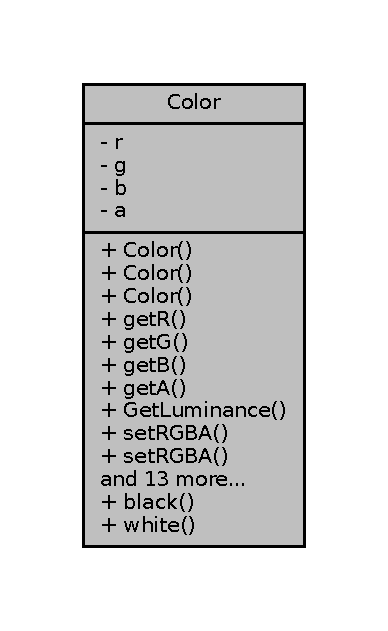
\includegraphics[width=186pt]{classColor__coll__graph}
\end{center}
\end{figure}
\subsection*{Public Member Functions}
\begin{DoxyCompactItemize}
\item 
\mbox{\Hypertarget{classColor_a9a742cbe9f9f4037f5d9f4e81a9b2428}\label{classColor_a9a742cbe9f9f4037f5d9f4e81a9b2428}} 
\hyperlink{classColor_a9a742cbe9f9f4037f5d9f4e81a9b2428}{Color} ()
\begin{DoxyCompactList}\small\item\em Constructor for no arguments. \end{DoxyCompactList}\item 
\mbox{\Hypertarget{classColor_a373c542c99fb83ce9c7c08aae76b2718}\label{classColor_a373c542c99fb83ce9c7c08aae76b2718}} 
\hyperlink{classColor_a373c542c99fb83ce9c7c08aae76b2718}{Color} (float r, float g, float b)
\begin{DoxyCompactList}\small\item\em Constructor for float red, float green, and float blue arguments. \end{DoxyCompactList}\item 
\mbox{\Hypertarget{classColor_a6e4627389673c8b5cce81bf3eec79938}\label{classColor_a6e4627389673c8b5cce81bf3eec79938}} 
\hyperlink{classColor_a6e4627389673c8b5cce81bf3eec79938}{Color} (float r, float g, float b, float a)
\begin{DoxyCompactList}\small\item\em Constructor for float red, float green, float blue, and float alpha arguments. \end{DoxyCompactList}\item 
float \hyperlink{classColor_a65df51367c71b8d2147e1db240e62429}{getR} ()
\begin{DoxyCompactList}\small\item\em Red value getter. \end{DoxyCompactList}\item 
float \hyperlink{classColor_a5c32d43f4405ace1cdb1cd0e32593e1a}{getG} ()
\begin{DoxyCompactList}\small\item\em Green value getter. \end{DoxyCompactList}\item 
float \hyperlink{classColor_a099852b0829e9551169a90768146e61e}{getB} ()
\begin{DoxyCompactList}\small\item\em Blue value getter. \end{DoxyCompactList}\item 
float \hyperlink{classColor_a3bd02605f19eb70590822131bcdd8b08}{getA} ()
\begin{DoxyCompactList}\small\item\em Alpha value getter. \end{DoxyCompactList}\item 
float \hyperlink{classColor_a44b18556e2cc4cd58e3f5f35471262b5}{Get\+Luminance} ()
\begin{DoxyCompactList}\small\item\em Luminance getter. \end{DoxyCompactList}\item 
\mbox{\Hypertarget{classColor_a8522aad9a86d305f7414ce26b50b48c2}\label{classColor_a8522aad9a86d305f7414ce26b50b48c2}} 
void \hyperlink{classColor_a8522aad9a86d305f7414ce26b50b48c2}{set\+R\+G\+BA} (unsigned char $\ast$pixel)
\begin{DoxyCompactList}\small\item\em R\+G\+BA setter given unsigned char aray of pixels. \end{DoxyCompactList}\item 
\mbox{\Hypertarget{classColor_a108cd7208329ed0bb1b52f6901150e40}\label{classColor_a108cd7208329ed0bb1b52f6901150e40}} 
void \hyperlink{classColor_a108cd7208329ed0bb1b52f6901150e40}{set\+R\+G\+BA} (float r, float g, float b, float a)
\begin{DoxyCompactList}\small\item\em R\+G\+BA setter given float values for r,g,b, and a. \end{DoxyCompactList}\item 
\mbox{\Hypertarget{classColor_ac6b45342df92b65e204fe83db9360e13}\label{classColor_ac6b45342df92b65e204fe83db9360e13}} 
void \hyperlink{classColor_ac6b45342df92b65e204fe83db9360e13}{setR} (float r)
\begin{DoxyCompactList}\small\item\em Red setter. \end{DoxyCompactList}\item 
\mbox{\Hypertarget{classColor_aa56d9de92a31ec8d647d1e4ec788789a}\label{classColor_aa56d9de92a31ec8d647d1e4ec788789a}} 
void \hyperlink{classColor_aa56d9de92a31ec8d647d1e4ec788789a}{setG} (float g)
\begin{DoxyCompactList}\small\item\em Green setter. \end{DoxyCompactList}\item 
\mbox{\Hypertarget{classColor_a42cac7186652ca335a08f6350e7e1e6a}\label{classColor_a42cac7186652ca335a08f6350e7e1e6a}} 
void \hyperlink{classColor_a42cac7186652ca335a08f6350e7e1e6a}{setB} (float b)
\begin{DoxyCompactList}\small\item\em Blue setter. \end{DoxyCompactList}\item 
\mbox{\Hypertarget{classColor_a3b254399aace09b24197673f060d868c}\label{classColor_a3b254399aace09b24197673f060d868c}} 
void \hyperlink{classColor_a3b254399aace09b24197673f060d868c}{setA} (float a)
\begin{DoxyCompactList}\small\item\em Alpha setter. \end{DoxyCompactList}\item 
\mbox{\Hypertarget{classColor_afa7cf91dee89475b96423a0eea0d079d}\label{classColor_afa7cf91dee89475b96423a0eea0d079d}} 
void \hyperlink{classColor_afa7cf91dee89475b96423a0eea0d079d}{Clear} ()
\begin{DoxyCompactList}\small\item\em Clear color function. \end{DoxyCompactList}\item 
\mbox{\Hypertarget{classColor_ac06dcf409ae64de5a67c7f6e69b6f44b}\label{classColor_ac06dcf409ae64de5a67c7f6e69b6f44b}} 
void \hyperlink{classColor_ac06dcf409ae64de5a67c7f6e69b6f44b}{operator=} (const \hyperlink{classColor}{Color} \&color)
\begin{DoxyCompactList}\small\item\em = operator given a \hyperlink{classColor}{Color} color \end{DoxyCompactList}\item 
\mbox{\Hypertarget{classColor_a76d829819622c7da1f39adbc9fcc8785}\label{classColor_a76d829819622c7da1f39adbc9fcc8785}} 
\hyperlink{classColor}{Color} \hyperlink{classColor_a76d829819622c7da1f39adbc9fcc8785}{operator+} (const \hyperlink{classColor}{Color} \&color)
\begin{DoxyCompactList}\small\item\em 
\begin{DoxyItemize}
\item operator given a \hyperlink{classColor}{Color} color 
\end{DoxyItemize}\end{DoxyCompactList}\item 
\mbox{\Hypertarget{classColor_a81e6990064f809bf8d0cc63a5e3300c6}\label{classColor_a81e6990064f809bf8d0cc63a5e3300c6}} 
\hyperlink{classColor}{Color} \hyperlink{classColor_a81e6990064f809bf8d0cc63a5e3300c6}{operator-\/} (const \hyperlink{classColor}{Color} \&color)
\begin{DoxyCompactList}\small\item\em 
\begin{DoxyItemize}
\item operator given a \hyperlink{classColor}{Color} color 
\end{DoxyItemize}\end{DoxyCompactList}\item 
\mbox{\Hypertarget{classColor_a1e5aa9e5811e7711ebfe997fa8b7accd}\label{classColor_a1e5aa9e5811e7711ebfe997fa8b7accd}} 
\hyperlink{classColor}{Color} \hyperlink{classColor_a1e5aa9e5811e7711ebfe997fa8b7accd}{operator$\ast$} (float scalar)
\begin{DoxyCompactList}\small\item\em 
\begin{DoxyItemize}
\item operator given a float scalar 
\end{DoxyItemize}\end{DoxyCompactList}\item 
\mbox{\Hypertarget{classColor_abd8c55279f5b9442ee149c7d670f32ad}\label{classColor_abd8c55279f5b9442ee149c7d670f32ad}} 
\hyperlink{classColor}{Color} \hyperlink{classColor_abd8c55279f5b9442ee149c7d670f32ad}{operator$\ast$} (const \hyperlink{classColor}{Color} \&color)
\begin{DoxyCompactList}\small\item\em 
\begin{DoxyItemize}
\item operator given a \hyperlink{classColor}{Color} color 
\end{DoxyItemize}\end{DoxyCompactList}\item 
\mbox{\Hypertarget{classColor_a7ef1308bd6371f7816607fd7f00c4ed2}\label{classColor_a7ef1308bd6371f7816607fd7f00c4ed2}} 
\hyperlink{classColor}{Color} \hyperlink{classColor_a7ef1308bd6371f7816607fd7f00c4ed2}{operator/} (float scalar)
\begin{DoxyCompactList}\small\item\em / operator given a float scalar \end{DoxyCompactList}\item 
\mbox{\Hypertarget{classColor_a493d3257d936fd306de590de1d7a0b21}\label{classColor_a493d3257d936fd306de590de1d7a0b21}} 
int \hyperlink{classColor_a493d3257d936fd306de590de1d7a0b21}{operator==} (const \hyperlink{classColor}{Color} \&color)
\begin{DoxyCompactList}\small\item\em equality operator for color variables \end{DoxyCompactList}\item 
\mbox{\Hypertarget{classColor_af896082b138401e97e14bc72d6ef6285}\label{classColor_af896082b138401e97e14bc72d6ef6285}} 
int \hyperlink{classColor_af896082b138401e97e14bc72d6ef6285}{operator!=} (const \hyperlink{classColor}{Color} \&color)
\begin{DoxyCompactList}\small\item\em opposite of equality operator for color variables \end{DoxyCompactList}\end{DoxyCompactItemize}
\subsection*{Static Public Member Functions}
\begin{DoxyCompactItemize}
\item 
\mbox{\Hypertarget{classColor_aba1c3be96b5e25fbae9c769d3491e333}\label{classColor_aba1c3be96b5e25fbae9c769d3491e333}} 
static \hyperlink{classColor}{Color} \hyperlink{classColor_aba1c3be96b5e25fbae9c769d3491e333}{black} ()
\begin{DoxyCompactList}\small\item\em \hyperlink{classColor}{Color} black. \end{DoxyCompactList}\item 
\mbox{\Hypertarget{classColor_aad4699ae003d7a86b5edc5fccdbaf4c8}\label{classColor_aad4699ae003d7a86b5edc5fccdbaf4c8}} 
static \hyperlink{classColor}{Color} \hyperlink{classColor_aad4699ae003d7a86b5edc5fccdbaf4c8}{white} ()
\begin{DoxyCompactList}\small\item\em \hyperlink{classColor}{Color} white. \end{DoxyCompactList}\end{DoxyCompactItemize}
\subsection*{Private Attributes}
\begin{DoxyCompactItemize}
\item 
\mbox{\Hypertarget{classColor_a3958a556b47d2de3dd45c75aac833c20}\label{classColor_a3958a556b47d2de3dd45c75aac833c20}} 
float {\bfseries r}
\item 
\mbox{\Hypertarget{classColor_a5defbb21620e480e556181772d665f34}\label{classColor_a5defbb21620e480e556181772d665f34}} 
float {\bfseries g}
\item 
\mbox{\Hypertarget{classColor_a33e482be18d6ea31d2b403bee13683b7}\label{classColor_a33e482be18d6ea31d2b403bee13683b7}} 
float {\bfseries b}
\item 
\mbox{\Hypertarget{classColor_a98047aee65fc3d825f88a76da728fd27}\label{classColor_a98047aee65fc3d825f88a76da728fd27}} 
float {\bfseries a}
\end{DoxyCompactItemize}


\subsection{Detailed Description}
The main class for \hyperlink{classColor}{Color}. We used a color class to make operations for color arithmatic easier. This makes it easy to add mutliply and set colors equal to eachother. The color class also makes it easy to get access to comonly used colors like black and white. 

\subsection{Member Function Documentation}
\mbox{\Hypertarget{classColor_a3bd02605f19eb70590822131bcdd8b08}\label{classColor_a3bd02605f19eb70590822131bcdd8b08}} 
\index{Color@{Color}!getA@{getA}}
\index{getA@{getA}!Color@{Color}}
\subsubsection{\texorpdfstring{get\+A()}{getA()}}
{\footnotesize\ttfamily float Color\+::getA (\begin{DoxyParamCaption}{ }\end{DoxyParamCaption})\hspace{0.3cm}{\ttfamily [inline]}}



Alpha value getter. 

\begin{DoxyReturn}{Returns}
Float alpha. 
\end{DoxyReturn}
\mbox{\Hypertarget{classColor_a099852b0829e9551169a90768146e61e}\label{classColor_a099852b0829e9551169a90768146e61e}} 
\index{Color@{Color}!getB@{getB}}
\index{getB@{getB}!Color@{Color}}
\subsubsection{\texorpdfstring{get\+B()}{getB()}}
{\footnotesize\ttfamily float Color\+::getB (\begin{DoxyParamCaption}{ }\end{DoxyParamCaption})\hspace{0.3cm}{\ttfamily [inline]}}



Blue value getter. 

\begin{DoxyReturn}{Returns}
Float blue. 
\end{DoxyReturn}
\mbox{\Hypertarget{classColor_a5c32d43f4405ace1cdb1cd0e32593e1a}\label{classColor_a5c32d43f4405ace1cdb1cd0e32593e1a}} 
\index{Color@{Color}!getG@{getG}}
\index{getG@{getG}!Color@{Color}}
\subsubsection{\texorpdfstring{get\+G()}{getG()}}
{\footnotesize\ttfamily float Color\+::getG (\begin{DoxyParamCaption}{ }\end{DoxyParamCaption})\hspace{0.3cm}{\ttfamily [inline]}}



Green value getter. 

\begin{DoxyReturn}{Returns}
Float green. 
\end{DoxyReturn}
\mbox{\Hypertarget{classColor_a44b18556e2cc4cd58e3f5f35471262b5}\label{classColor_a44b18556e2cc4cd58e3f5f35471262b5}} 
\index{Color@{Color}!Get\+Luminance@{Get\+Luminance}}
\index{Get\+Luminance@{Get\+Luminance}!Color@{Color}}
\subsubsection{\texorpdfstring{Get\+Luminance()}{GetLuminance()}}
{\footnotesize\ttfamily float Color\+::\+Get\+Luminance (\begin{DoxyParamCaption}{ }\end{DoxyParamCaption})\hspace{0.3cm}{\ttfamily [inline]}}



Luminance getter. 

\begin{DoxyReturn}{Returns}
Float luminance. 
\end{DoxyReturn}
\mbox{\Hypertarget{classColor_a65df51367c71b8d2147e1db240e62429}\label{classColor_a65df51367c71b8d2147e1db240e62429}} 
\index{Color@{Color}!getR@{getR}}
\index{getR@{getR}!Color@{Color}}
\subsubsection{\texorpdfstring{get\+R()}{getR()}}
{\footnotesize\ttfamily float Color\+::getR (\begin{DoxyParamCaption}{ }\end{DoxyParamCaption})\hspace{0.3cm}{\ttfamily [inline]}}



Red value getter. 

\begin{DoxyReturn}{Returns}
Float red. 
\end{DoxyReturn}


The documentation for this class was generated from the following file\+:\begin{DoxyCompactItemize}
\item 
/home/user/repo/project/image/include/\hyperlink{color_8h}{color.\+h}\end{DoxyCompactItemize}

\hypertarget{classCompositeEntityFactory}{}\section{Composite\+Entity\+Factory Class Reference}
\label{classCompositeEntityFactory}\index{Composite\+Entity\+Factory@{Composite\+Entity\+Factory}}


Composite Entity Factory. This is the class that get\textquotesingle{}s called when creating new entities. Has an entity factory vector member variable to keep track of all the factories. Then when we want to create a new factory, it\textquotesingle{}s added to the vector to be referenced for entity creation.  




{\ttfamily \#include $<$composite\+\_\+entity\+\_\+factory.\+h$>$}



Inheritance diagram for Composite\+Entity\+Factory\+:\nopagebreak
\begin{figure}[H]
\begin{center}
\leavevmode
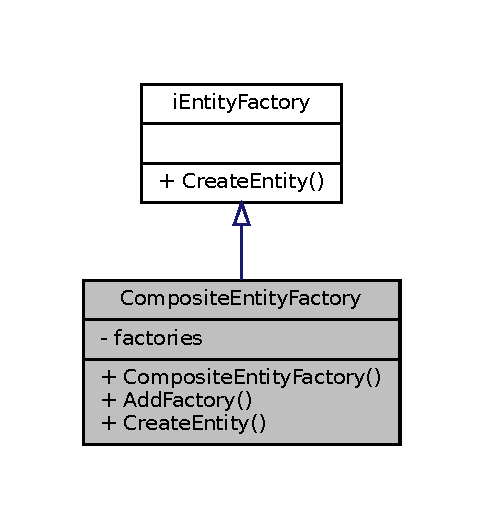
\includegraphics[width=232pt]{classCompositeEntityFactory__inherit__graph}
\end{center}
\end{figure}


Collaboration diagram for Composite\+Entity\+Factory\+:\nopagebreak
\begin{figure}[H]
\begin{center}
\leavevmode
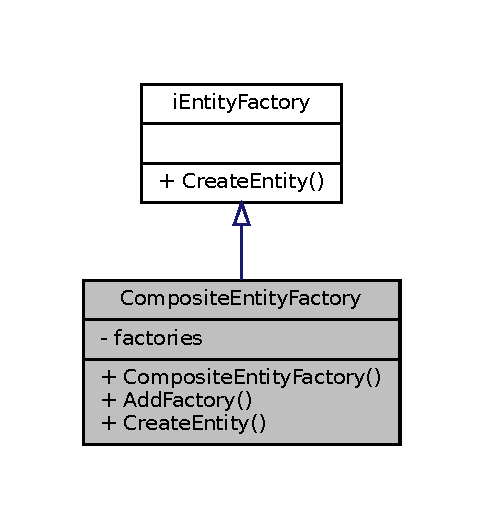
\includegraphics[width=232pt]{classCompositeEntityFactory__coll__graph}
\end{center}
\end{figure}
\subsection*{Public Member Functions}
\begin{DoxyCompactItemize}
\item 
\mbox{\Hypertarget{classCompositeEntityFactory_a6ecb6093a839b686c4693bf00713247f}\label{classCompositeEntityFactory_a6ecb6093a839b686c4693bf00713247f}} 
void \hyperlink{classCompositeEntityFactory_a6ecb6093a839b686c4693bf00713247f}{Add\+Factory} (\hyperlink{classiEntityFactory}{i\+Entity\+Factory} $\ast$factory)
\begin{DoxyCompactList}\small\item\em adds factory to vector. This vector is used to create entities of a specific type in the Create\+Entity function. \end{DoxyCompactList}\item 
\mbox{\Hypertarget{classCompositeEntityFactory_a0f30a9a8443a04f0fa8f17a7bc2f0a58}\label{classCompositeEntityFactory_a0f30a9a8443a04f0fa8f17a7bc2f0a58}} 
\hyperlink{classiEntity}{i\+Entity} $\ast$ \hyperlink{classCompositeEntityFactory_a0f30a9a8443a04f0fa8f17a7bc2f0a58}{Create\+Entity} (picojson\+::object \&entity, \hyperlink{classCamera}{Camera} $\ast$camera)
\begin{DoxyCompactList}\small\item\em loops through vector of entity factories creating new entities until a null pointer isn\textquotesingle{}t returned. If the object doesn\textquotesingle{}t match the factory called, then they return null pointers. \end{DoxyCompactList}\end{DoxyCompactItemize}
\subsection*{Private Attributes}
\begin{DoxyCompactItemize}
\item 
\mbox{\Hypertarget{classCompositeEntityFactory_a7dec8bde43fb44220a757c45eaa00435}\label{classCompositeEntityFactory_a7dec8bde43fb44220a757c45eaa00435}} 
std\+::list$<$ \hyperlink{classiEntityFactory}{i\+Entity\+Factory} $\ast$ $>$ \hyperlink{classCompositeEntityFactory_a7dec8bde43fb44220a757c45eaa00435}{factories}
\begin{DoxyCompactList}\small\item\em vector of \hyperlink{classiEntityFactory}{i\+Entity\+Factory} pointers \end{DoxyCompactList}\end{DoxyCompactItemize}


\subsection{Detailed Description}
Composite Entity Factory. This is the class that get\textquotesingle{}s called when creating new entities. Has an entity factory vector member variable to keep track of all the factories. Then when we want to create a new factory, it\textquotesingle{}s added to the vector to be referenced for entity creation. 

The documentation for this class was generated from the following files\+:\begin{DoxyCompactItemize}
\item 
/home/user/repo/project/simulation/include/\hyperlink{composite__entity__factory_8h}{composite\+\_\+entity\+\_\+factory.\+h}\item 
/home/user/repo/project/simulation/src/composite\+\_\+entity\+\_\+factory.\+cc\end{DoxyCompactItemize}

\hypertarget{classCompositeLogger}{}\section{Composite\+Logger Class Reference}
\label{classCompositeLogger}\index{Composite\+Logger@{Composite\+Logger}}


composite logger that uses our other two terminal / csv loggers to record data  




{\ttfamily \#include $<$composite\+\_\+logger.\+h$>$}



Inheritance diagram for Composite\+Logger\+:\nopagebreak
\begin{figure}[H]
\begin{center}
\leavevmode
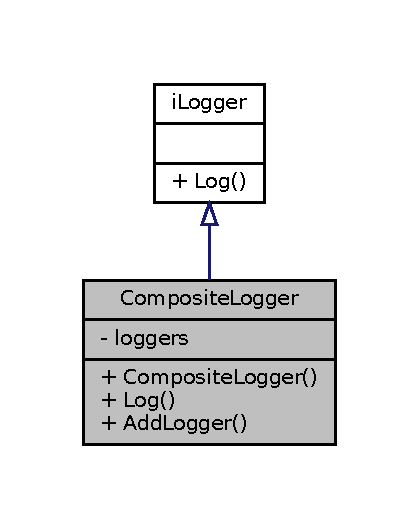
\includegraphics[width=201pt]{classCompositeLogger__inherit__graph}
\end{center}
\end{figure}


Collaboration diagram for Composite\+Logger\+:\nopagebreak
\begin{figure}[H]
\begin{center}
\leavevmode
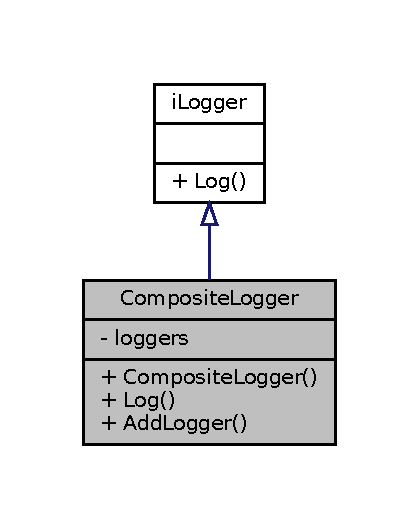
\includegraphics[width=201pt]{classCompositeLogger__coll__graph}
\end{center}
\end{figure}
\subsection*{Public Member Functions}
\begin{DoxyCompactItemize}
\item 
\mbox{\Hypertarget{classCompositeLogger_a10914598defb8bd5ab057508c831a031}\label{classCompositeLogger_a10914598defb8bd5ab057508c831a031}} 
\hyperlink{classCompositeLogger_a10914598defb8bd5ab057508c831a031}{Composite\+Logger} ()
\begin{DoxyCompactList}\small\item\em constructor. Adds loggers to our list member variable \end{DoxyCompactList}\item 
\mbox{\Hypertarget{classCompositeLogger_a84c0c034a72ddc1c7eeb3cfc47d1dcd5}\label{classCompositeLogger_a84c0c034a72ddc1c7eeb3cfc47d1dcd5}} 
void \hyperlink{classCompositeLogger_a84c0c034a72ddc1c7eeb3cfc47d1dcd5}{Log} (\hyperlink{classVector3}{Vector3} $\ast$p, \hyperlink{classVector3}{Vector3} $\ast$d, double t)
\begin{DoxyCompactList}\small\item\em log position of drone with message about it. Called every time we update. \end{DoxyCompactList}\item 
\mbox{\Hypertarget{classCompositeLogger_a8548bd7dc7fbba8627b7a760a1022867}\label{classCompositeLogger_a8548bd7dc7fbba8627b7a760a1022867}} 
void \hyperlink{classCompositeLogger_a8548bd7dc7fbba8627b7a760a1022867}{Add\+Logger} (\hyperlink{classiLogger}{i\+Logger} $\ast$logger)
\begin{DoxyCompactList}\small\item\em adds a new logger to our list member variable \end{DoxyCompactList}\end{DoxyCompactItemize}
\subsection*{Private Attributes}
\begin{DoxyCompactItemize}
\item 
\mbox{\Hypertarget{classCompositeLogger_a7a74921303ccdead873c982e1a3ca59f}\label{classCompositeLogger_a7a74921303ccdead873c982e1a3ca59f}} 
std\+::list$<$ \hyperlink{classiLogger}{i\+Logger} $\ast$ $>$ \hyperlink{classCompositeLogger_a7a74921303ccdead873c982e1a3ca59f}{loggers}
\begin{DoxyCompactList}\small\item\em list of loggers used to record data \end{DoxyCompactList}\end{DoxyCompactItemize}


\subsection{Detailed Description}
composite logger that uses our other two terminal / csv loggers to record data 

The documentation for this class was generated from the following files\+:\begin{DoxyCompactItemize}
\item 
/home/user/repo/project/simulation/include/\hyperlink{composite__logger_8h}{composite\+\_\+logger.\+h}\item 
/home/user/repo/project/simulation/src/composite\+\_\+logger.\+cc\end{DoxyCompactItemize}

\hypertarget{classConsoleLogger}{}\section{Console\+Logger Class Reference}
\label{classConsoleLogger}\index{Console\+Logger@{Console\+Logger}}


Inheritance diagram for Console\+Logger\+:\nopagebreak
\begin{figure}[H]
\begin{center}
\leavevmode
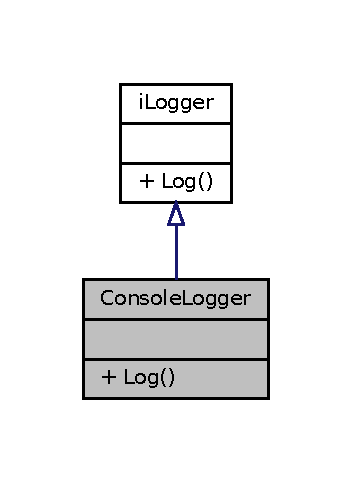
\includegraphics[width=169pt]{classConsoleLogger__inherit__graph}
\end{center}
\end{figure}


Collaboration diagram for Console\+Logger\+:\nopagebreak
\begin{figure}[H]
\begin{center}
\leavevmode
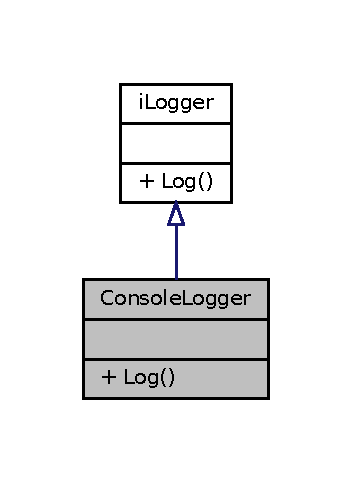
\includegraphics[width=169pt]{classConsoleLogger__coll__graph}
\end{center}
\end{figure}
\subsection*{Public Member Functions}
\begin{DoxyCompactItemize}
\item 
\mbox{\Hypertarget{classConsoleLogger_a6f3940bf33ee1e4dc814529624ed7241}\label{classConsoleLogger_a6f3940bf33ee1e4dc814529624ed7241}} 
void \hyperlink{classConsoleLogger_a6f3940bf33ee1e4dc814529624ed7241}{Log} (\hyperlink{classVector3}{Vector3} $\ast$p, \hyperlink{classVector3}{Vector3} $\ast$d, double t)
\begin{DoxyCompactList}\small\item\em prints position and direction vector data to terminal screen \end{DoxyCompactList}\end{DoxyCompactItemize}


The documentation for this class was generated from the following files\+:\begin{DoxyCompactItemize}
\item 
/home/user/repo/project/simulation/include/\hyperlink{console__logger_8h}{console\+\_\+logger.\+h}\item 
/home/user/repo/project/simulation/src/console\+\_\+logger.\+cc\end{DoxyCompactItemize}

\hypertarget{classConvolutionFilter}{}\section{Convolution\+Filter Class Reference}
\label{classConvolutionFilter}\index{Convolution\+Filter@{Convolution\+Filter}}


The main class for \hyperlink{classConvolutionFilter}{Convolution\+Filter}, extends \hyperlink{classFilter}{Filter}. A basic convolution filter implementation. Each child class will have it\textquotesingle{}s own kernel object and run the given apply kernel function. This class has a lot of extendability as long as the filter algorithm is the same.  




{\ttfamily \#include $<$convolution\+\_\+filter.\+h$>$}



Inheritance diagram for Convolution\+Filter\+:\nopagebreak
\begin{figure}[H]
\begin{center}
\leavevmode
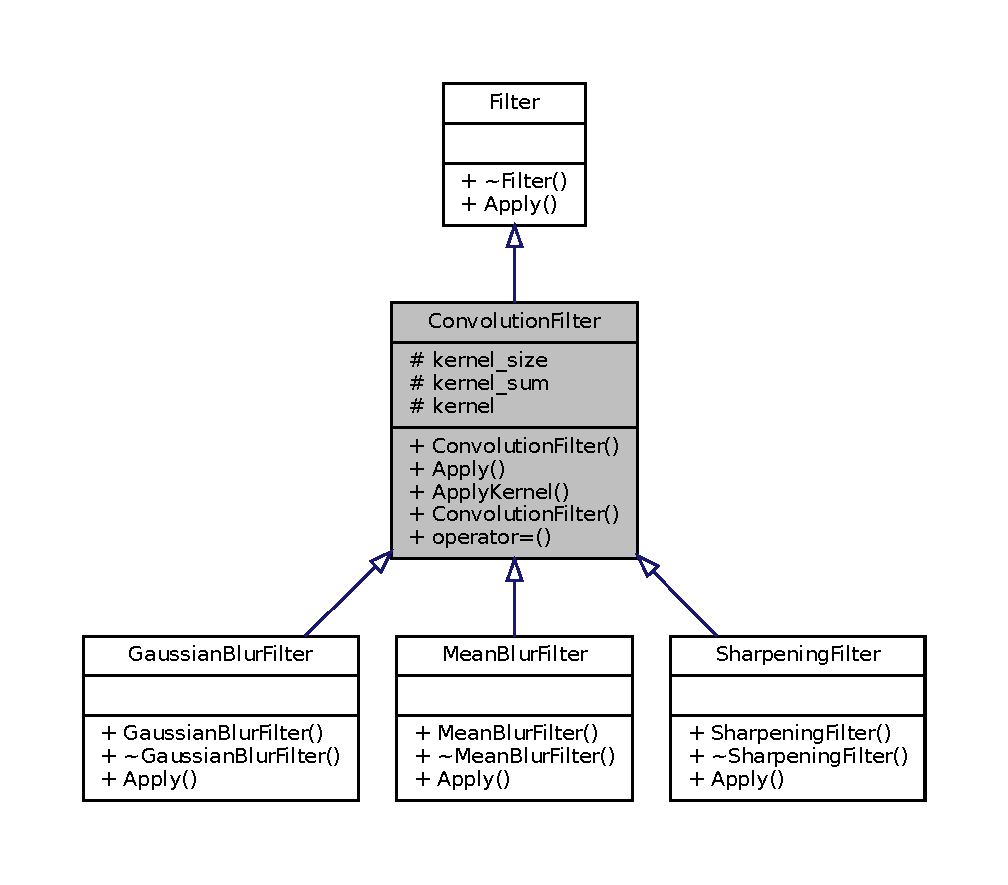
\includegraphics[width=350pt]{classConvolutionFilter__inherit__graph}
\end{center}
\end{figure}


Collaboration diagram for Convolution\+Filter\+:\nopagebreak
\begin{figure}[H]
\begin{center}
\leavevmode
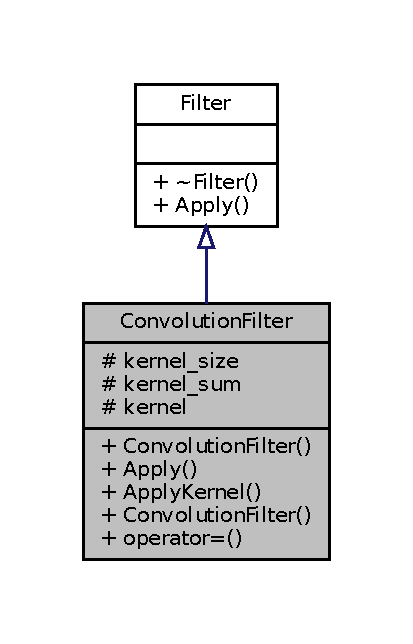
\includegraphics[width=198pt]{classConvolutionFilter__coll__graph}
\end{center}
\end{figure}
\subsection*{Public Member Functions}
\begin{DoxyCompactItemize}
\item 
\mbox{\Hypertarget{classConvolutionFilter_a55f8a3bbe4c93bf849b7eecd1531e8a7}\label{classConvolutionFilter_a55f8a3bbe4c93bf849b7eecd1531e8a7}} 
virtual void \hyperlink{classConvolutionFilter_a55f8a3bbe4c93bf849b7eecd1531e8a7}{Apply} (std\+::vector$<$ \hyperlink{classImage}{Image} $\ast$$>$ original, std\+::vector$<$ \hyperlink{classImage}{Image} $\ast$$>$ filtered)=0
\begin{DoxyCompactList}\small\item\em The method inherited convolution filters call Apply\+Kernel in. \end{DoxyCompactList}\item 
\mbox{\Hypertarget{classConvolutionFilter_af37f2a6e6c7e9f95cf769494a5227b0d}\label{classConvolutionFilter_af37f2a6e6c7e9f95cf769494a5227b0d}} 
void \hyperlink{classConvolutionFilter_af37f2a6e6c7e9f95cf769494a5227b0d}{Apply\+Kernel} (std\+::vector$<$ \hyperlink{classImage}{Image} $\ast$$>$ original, std\+::vector$<$ \hyperlink{classImage}{Image} $\ast$$>$ filtered)
\begin{DoxyCompactList}\small\item\em The apply kernel algorithm. This function will work on any input images and run the kernel of the given size on the images. It now implements a fast Fourier transform algorithm to convolve our image in a faster exponential time. \end{DoxyCompactList}\item 
\mbox{\Hypertarget{classConvolutionFilter_a2750951441b1fceb7006192396a706ed}\label{classConvolutionFilter_a2750951441b1fceb7006192396a706ed}} 
\hyperlink{classConvolutionFilter_a2750951441b1fceb7006192396a706ed}{Convolution\+Filter} (const \hyperlink{classConvolutionFilter}{Convolution\+Filter} \&filter)
\begin{DoxyCompactList}\small\item\em Copy constructor Uses the = operator to simplify the function. \end{DoxyCompactList}\item 
\mbox{\Hypertarget{classConvolutionFilter_a8430a9858e927d8c8cdc5e0b500d1b40}\label{classConvolutionFilter_a8430a9858e927d8c8cdc5e0b500d1b40}} 
void \hyperlink{classConvolutionFilter_a8430a9858e927d8c8cdc5e0b500d1b40}{operator=} (const \hyperlink{classConvolutionFilter}{Convolution\+Filter} \&filter)
\begin{DoxyCompactList}\small\item\em Operator =. \end{DoxyCompactList}\end{DoxyCompactItemize}
\subsection*{Protected Attributes}
\begin{DoxyCompactItemize}
\item 
\mbox{\Hypertarget{classConvolutionFilter_aece66da70dad07df42e28623a5f6074d}\label{classConvolutionFilter_aece66da70dad07df42e28623a5f6074d}} 
int {\bfseries kernel\+\_\+size}
\item 
\mbox{\Hypertarget{classConvolutionFilter_a9ee9eaa3837d893ad7b304219511d8e5}\label{classConvolutionFilter_a9ee9eaa3837d893ad7b304219511d8e5}} 
double {\bfseries kernel\+\_\+sum}
\item 
\mbox{\Hypertarget{classConvolutionFilter_a57740ec890c05384b20d4a7ba17b4513}\label{classConvolutionFilter_a57740ec890c05384b20d4a7ba17b4513}} 
double $\ast$ {\bfseries kernel}
\end{DoxyCompactItemize}


\subsection{Detailed Description}
The main class for \hyperlink{classConvolutionFilter}{Convolution\+Filter}, extends \hyperlink{classFilter}{Filter}. A basic convolution filter implementation. Each child class will have it\textquotesingle{}s own kernel object and run the given apply kernel function. This class has a lot of extendability as long as the filter algorithm is the same. 

The documentation for this class was generated from the following file\+:\begin{DoxyCompactItemize}
\item 
/home/user/repo/project/image/include/convolution\+\_\+filter.\+h\end{DoxyCompactItemize}

\hypertarget{classCSVLogger}{}\section{C\+S\+V\+Logger Class Reference}
\label{classCSVLogger}\index{C\+S\+V\+Logger@{C\+S\+V\+Logger}}


logger for csv files. Puts vector information and strategy time information in a comma separated file.  




{\ttfamily \#include $<$csv\+\_\+logger.\+h$>$}



Inheritance diagram for C\+S\+V\+Logger\+:\nopagebreak
\begin{figure}[H]
\begin{center}
\leavevmode
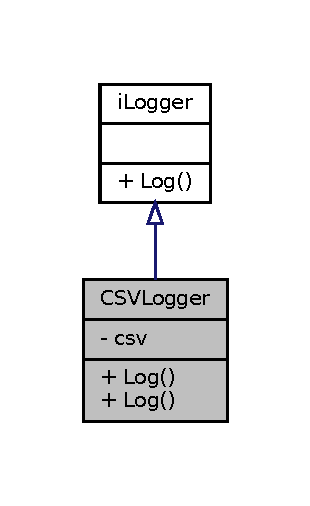
\includegraphics[width=149pt]{classCSVLogger__inherit__graph}
\end{center}
\end{figure}


Collaboration diagram for C\+S\+V\+Logger\+:\nopagebreak
\begin{figure}[H]
\begin{center}
\leavevmode
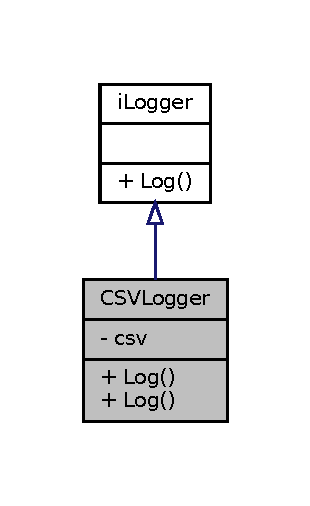
\includegraphics[width=149pt]{classCSVLogger__coll__graph}
\end{center}
\end{figure}
\subsection*{Public Member Functions}
\begin{DoxyCompactItemize}
\item 
\mbox{\Hypertarget{classCSVLogger_a6f6f8cce2294cf48ebfcee86d5afd365}\label{classCSVLogger_a6f6f8cce2294cf48ebfcee86d5afd365}} 
void \hyperlink{classCSVLogger_a6f6f8cce2294cf48ebfcee86d5afd365}{Log} (\hyperlink{classVector3}{Vector3} $\ast$p, \hyperlink{classVector3}{Vector3} $\ast$d, double t, std\+::string msg)
\begin{DoxyCompactList}\small\item\em logs position, direction, and time to csv file, along with an inputted message \end{DoxyCompactList}\item 
\mbox{\Hypertarget{classCSVLogger_ae59e4258b85bfb18452c6e37d4623257}\label{classCSVLogger_ae59e4258b85bfb18452c6e37d4623257}} 
void \hyperlink{classCSVLogger_ae59e4258b85bfb18452c6e37d4623257}{Log} (\hyperlink{classVector3}{Vector3} $\ast$p, \hyperlink{classVector3}{Vector3} $\ast$d, double t)
\begin{DoxyCompactList}\small\item\em same as the other logger command, but adds \char`\"{}\+N/\+A\char`\"{} for message \end{DoxyCompactList}\end{DoxyCompactItemize}
\subsection*{Private Attributes}
\begin{DoxyCompactItemize}
\item 
\mbox{\Hypertarget{classCSVLogger_a088a4194c2d461ca1e9561fd4283471b}\label{classCSVLogger_a088a4194c2d461ca1e9561fd4283471b}} 
std\+::ofstream {\bfseries csv}
\end{DoxyCompactItemize}


\subsection{Detailed Description}
logger for csv files. Puts vector information and strategy time information in a comma separated file. 

The documentation for this class was generated from the following files\+:\begin{DoxyCompactItemize}
\item 
/home/user/repo/project/simulation/include/\hyperlink{csv__logger_8h}{csv\+\_\+logger.\+h}\item 
/home/user/repo/project/simulation/src/csv\+\_\+logger.\+cc\end{DoxyCompactItemize}

\hypertarget{classDeapthFirstSearch}{}\section{Deapth\+First\+Search Class Reference}
\label{classDeapthFirstSearch}\index{Deapth\+First\+Search@{Deapth\+First\+Search}}


Inheritance diagram for Deapth\+First\+Search\+:\nopagebreak
\begin{figure}[H]
\begin{center}
\leavevmode
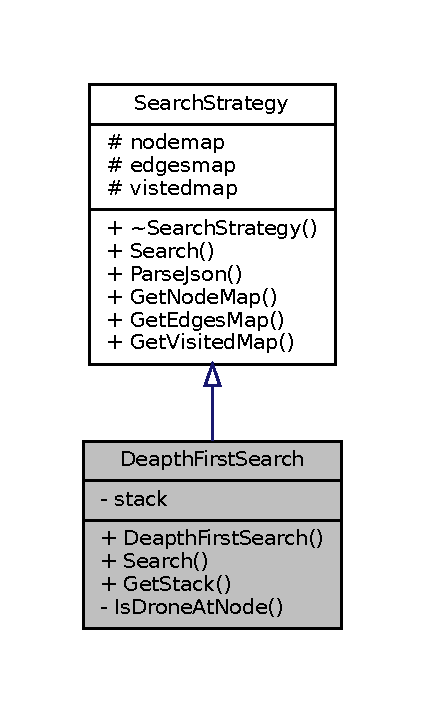
\includegraphics[width=204pt]{classDeapthFirstSearch__inherit__graph}
\end{center}
\end{figure}


Collaboration diagram for Deapth\+First\+Search\+:\nopagebreak
\begin{figure}[H]
\begin{center}
\leavevmode
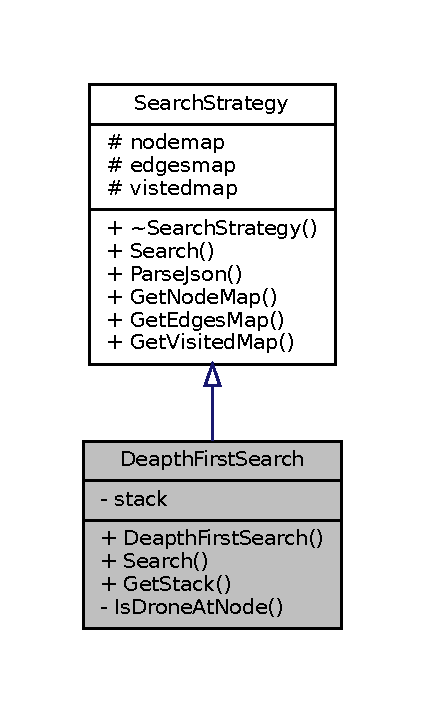
\includegraphics[width=204pt]{classDeapthFirstSearch__coll__graph}
\end{center}
\end{figure}
\subsection*{Public Member Functions}
\begin{DoxyCompactItemize}
\item 
\mbox{\Hypertarget{classDeapthFirstSearch_a17caed70389b812d14cdcada7c2e7e21}\label{classDeapthFirstSearch_a17caed70389b812d14cdcada7c2e7e21}} 
\hyperlink{classDeapthFirstSearch_a17caed70389b812d14cdcada7c2e7e21}{Deapth\+First\+Search} ()
\begin{DoxyCompactList}\small\item\em default constructor \end{DoxyCompactList}\item 
\mbox{\Hypertarget{classDeapthFirstSearch_a3301b804af1bf6958170856d0ddbd017}\label{classDeapthFirstSearch_a3301b804af1bf6958170856d0ddbd017}} 
\hyperlink{classVector3}{Vector3} $\ast$ \hyperlink{classDeapthFirstSearch_a3301b804af1bf6958170856d0ddbd017}{Search} (\hyperlink{classVector3}{Vector3} current\+Pos)
\begin{DoxyCompactList}\small\item\em Searching function for Depth First Search. \end{DoxyCompactList}\item 
\mbox{\Hypertarget{classDeapthFirstSearch_ad5f374df061fd67a715130396f06c29a}\label{classDeapthFirstSearch_ad5f374df061fd67a715130396f06c29a}} 
std\+::stack$<$ std\+::string $>$ {\bfseries Get\+Stack} ()
\end{DoxyCompactItemize}
\subsection*{Private Member Functions}
\begin{DoxyCompactItemize}
\item 
\mbox{\Hypertarget{classDeapthFirstSearch_aa1a9887380527839af4964c69984ecf0}\label{classDeapthFirstSearch_aa1a9887380527839af4964c69984ecf0}} 
bool \hyperlink{classDeapthFirstSearch_aa1a9887380527839af4964c69984ecf0}{Is\+Drone\+At\+Node} (\hyperlink{classVector3}{Vector3} current\+Pos, std\+::string v)
\begin{DoxyCompactList}\small\item\em Private bool to see the the drone is currently at the expected node or not. \end{DoxyCompactList}\end{DoxyCompactItemize}
\subsection*{Private Attributes}
\begin{DoxyCompactItemize}
\item 
\mbox{\Hypertarget{classDeapthFirstSearch_a9aaa9441b4c7945e13dadfc5f33179b6}\label{classDeapthFirstSearch_a9aaa9441b4c7945e13dadfc5f33179b6}} 
std\+::stack$<$ std\+::string $>$ \hyperlink{classDeapthFirstSearch_a9aaa9441b4c7945e13dadfc5f33179b6}{stack}
\begin{DoxyCompactList}\small\item\em stack for Deapth First Search searching. \end{DoxyCompactList}\end{DoxyCompactItemize}
\subsection*{Additional Inherited Members}


The documentation for this class was generated from the following files\+:\begin{DoxyCompactItemize}
\item 
/home/user/repo/project/simulation/include/\hyperlink{deapth__first__search_8h}{deapth\+\_\+first\+\_\+search.\+h}\item 
/home/user/repo/project/simulation/src/deapth\+\_\+first\+\_\+search.\+cc\end{DoxyCompactItemize}

\hypertarget{classDoubleThresholdFilter}{}\section{Double\+Threshold\+Filter Class Reference}
\label{classDoubleThresholdFilter}\index{Double\+Threshold\+Filter@{Double\+Threshold\+Filter}}


Double Threshold takes in the value of the each pixel and decides if it is a strong or weak pixel based off of its luminencence. It has a strong threshold which makes if white, and a weak threshold that makes it grey.  




{\ttfamily \#include $<$double\+\_\+threshold\+\_\+filter.\+h$>$}



Inheritance diagram for Double\+Threshold\+Filter\+:\nopagebreak
\begin{figure}[H]
\begin{center}
\leavevmode
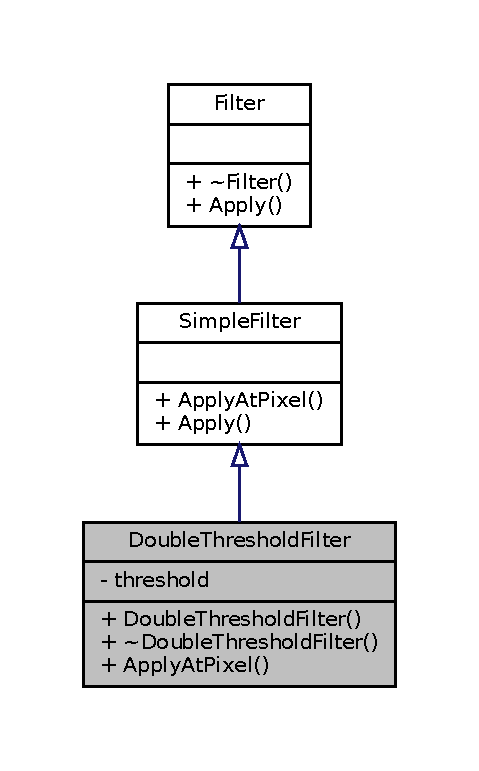
\includegraphics[width=230pt]{classDoubleThresholdFilter__inherit__graph}
\end{center}
\end{figure}


Collaboration diagram for Double\+Threshold\+Filter\+:\nopagebreak
\begin{figure}[H]
\begin{center}
\leavevmode
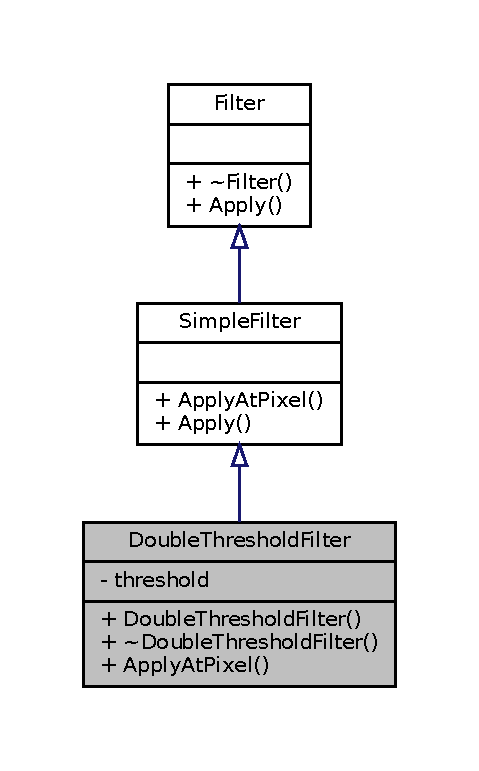
\includegraphics[width=230pt]{classDoubleThresholdFilter__coll__graph}
\end{center}
\end{figure}
\subsection*{Public Member Functions}
\begin{DoxyCompactItemize}
\item 
\mbox{\Hypertarget{classDoubleThresholdFilter_ae4c841df681b376c611e2bc07a2a0d54}\label{classDoubleThresholdFilter_ae4c841df681b376c611e2bc07a2a0d54}} 
\hyperlink{classDoubleThresholdFilter_ae4c841df681b376c611e2bc07a2a0d54}{Double\+Threshold\+Filter} ()
\begin{DoxyCompactList}\small\item\em Constructor. \end{DoxyCompactList}\item 
\mbox{\Hypertarget{classDoubleThresholdFilter_a5ebad435bdc4bfa13a936fdf243cb974}\label{classDoubleThresholdFilter_a5ebad435bdc4bfa13a936fdf243cb974}} 
\hyperlink{classDoubleThresholdFilter_a5ebad435bdc4bfa13a936fdf243cb974}{$\sim$\+Double\+Threshold\+Filter} ()
\begin{DoxyCompactList}\small\item\em Destructor. \end{DoxyCompactList}\item 
\mbox{\Hypertarget{classDoubleThresholdFilter_a5d4cf6bca3324acb39859293ac6e23d3}\label{classDoubleThresholdFilter_a5d4cf6bca3324acb39859293ac6e23d3}} 
void \hyperlink{classDoubleThresholdFilter_a5d4cf6bca3324acb39859293ac6e23d3}{Apply\+At\+Pixel} (\hyperlink{classColor}{Color} \&p)
\begin{DoxyCompactList}\small\item\em Apply\+At\+Pixel function to be overridden by \hyperlink{classSimpleFilter}{Simple\+Filter} Apply function. \end{DoxyCompactList}\end{DoxyCompactItemize}
\subsection*{Private Attributes}
\begin{DoxyCompactItemize}
\item 
\mbox{\Hypertarget{classDoubleThresholdFilter_a4efd024772e0a0f61ed7cd7bcdd9fabe}\label{classDoubleThresholdFilter_a4efd024772e0a0f61ed7cd7bcdd9fabe}} 
float {\bfseries threshold}
\end{DoxyCompactItemize}


\subsection{Detailed Description}
Double Threshold takes in the value of the each pixel and decides if it is a strong or weak pixel based off of its luminencence. It has a strong threshold which makes if white, and a weak threshold that makes it grey. 

The documentation for this class was generated from the following files\+:\begin{DoxyCompactItemize}
\item 
/home/user/repo/project/image/include/\hyperlink{double__threshold__filter_8h}{double\+\_\+threshold\+\_\+filter.\+h}\item 
/home/user/repo/project/image/src/double\+\_\+threshold\+\_\+filter.\+cc\end{DoxyCompactItemize}

\hypertarget{classDrone}{}\section{Drone Class Reference}
\label{classDrone}\index{Drone@{Drone}}


Our actual drone that will be searching for the robot. Contains tons methods to update postion and velocity. Also has many search patterns to find the target robot.  




{\ttfamily \#include $<$drone.\+h$>$}



Inheritance diagram for Drone\+:\nopagebreak
\begin{figure}[H]
\begin{center}
\leavevmode
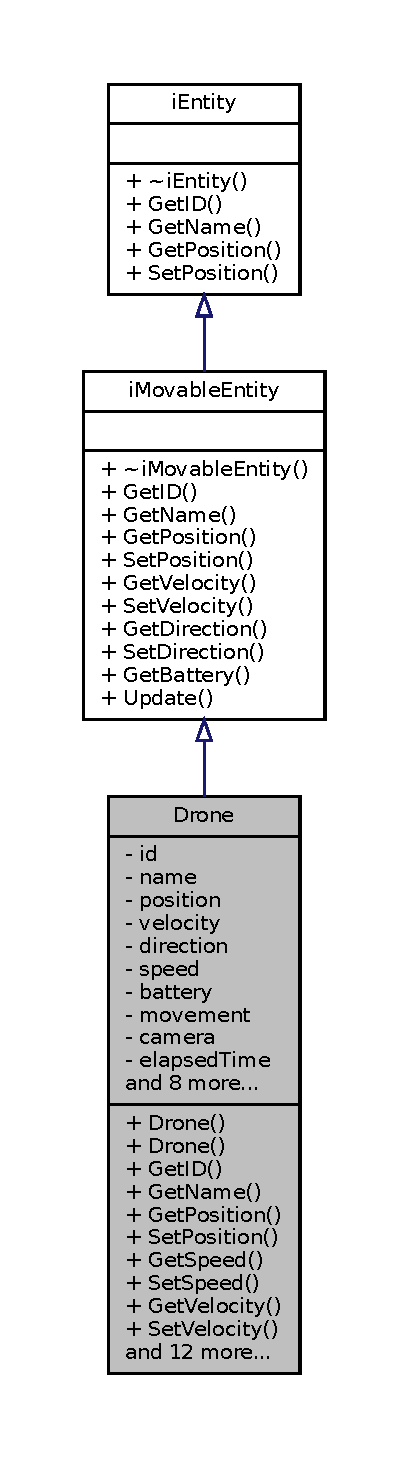
\includegraphics[height=550pt]{classDrone__inherit__graph}
\end{center}
\end{figure}


Collaboration diagram for Drone\+:\nopagebreak
\begin{figure}[H]
\begin{center}
\leavevmode
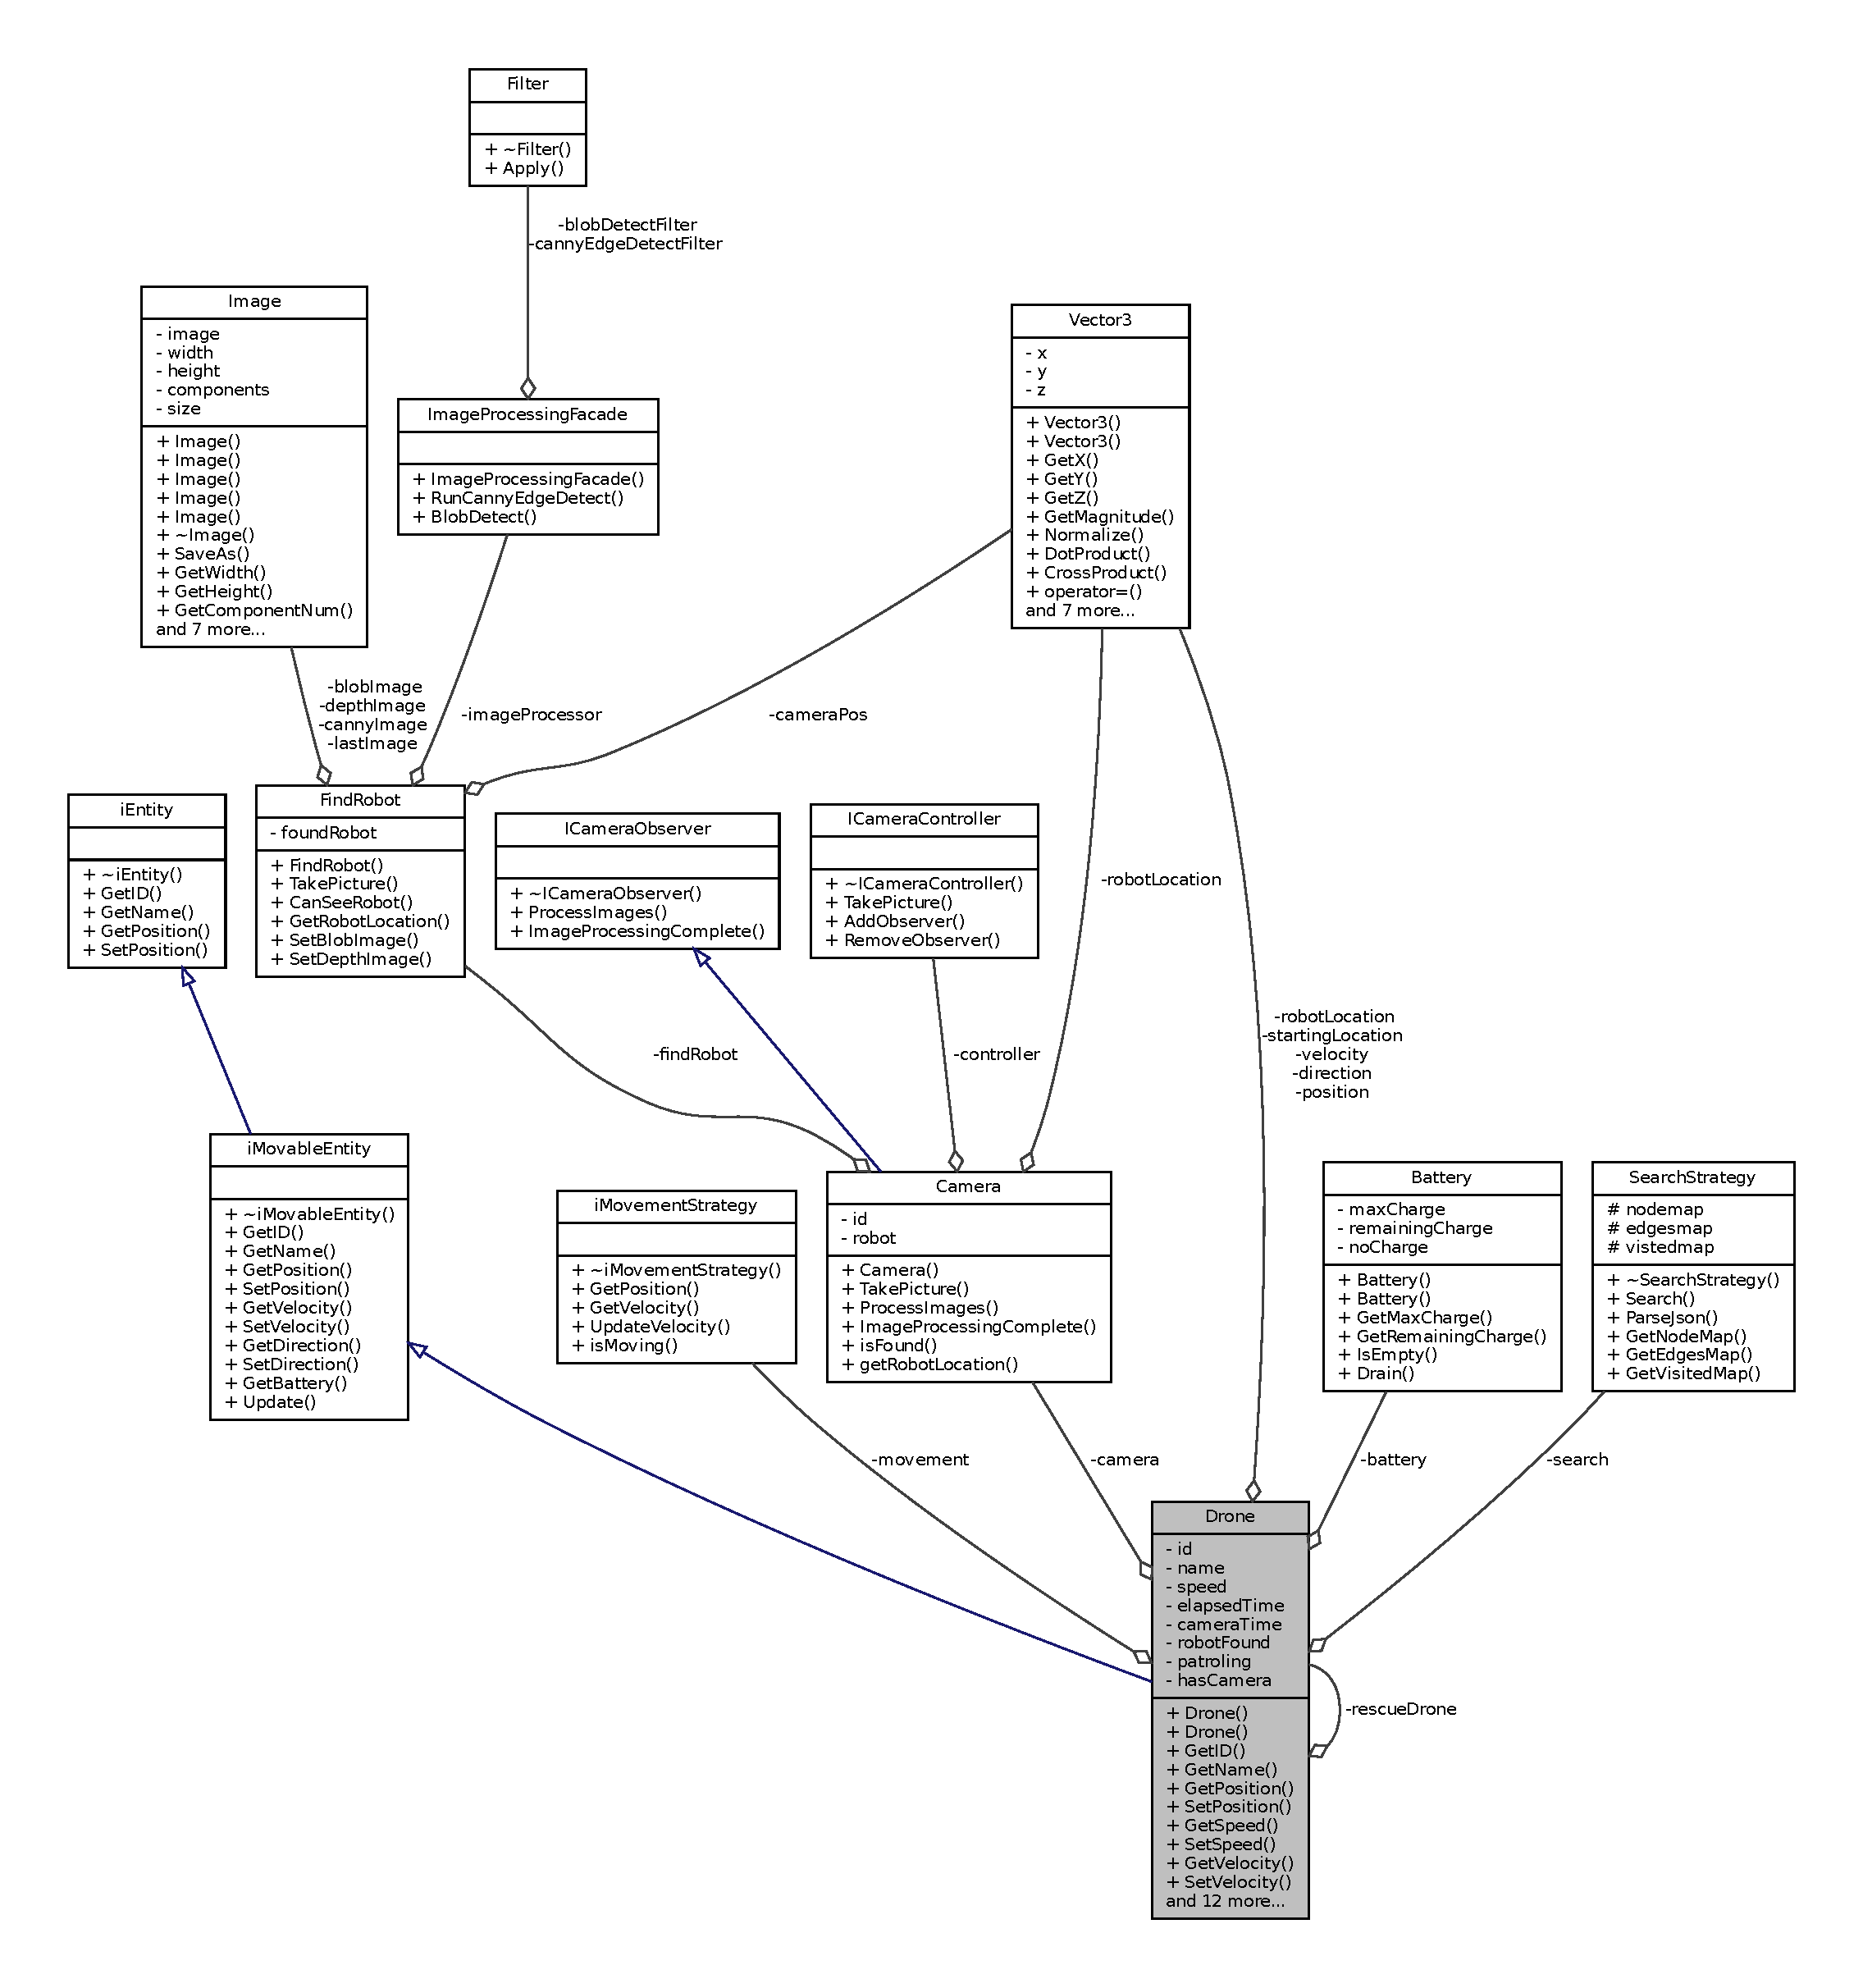
\includegraphics[width=350pt]{classDrone__coll__graph}
\end{center}
\end{figure}
\subsection*{Public Member Functions}
\begin{DoxyCompactItemize}
\item 
\mbox{\Hypertarget{classDrone_ab692baa4be5c43b72990ce1b01bdc805}\label{classDrone_ab692baa4be5c43b72990ce1b01bdc805}} 
\hyperlink{classDrone_ab692baa4be5c43b72990ce1b01bdc805}{Drone} ()
\begin{DoxyCompactList}\small\item\em default constructor \end{DoxyCompactList}\item 
\mbox{\Hypertarget{classDrone_a8847d17aacd1efc2b64827de2b58c4c7}\label{classDrone_a8847d17aacd1efc2b64827de2b58c4c7}} 
\hyperlink{classDrone_a8847d17aacd1efc2b64827de2b58c4c7}{Drone} (int \hyperlink{classDrone_a5aa543be4e70c00b14a38fef06bf6166}{id}, std\+::string \hyperlink{classDrone_ac5f6c269378659247acd057142542013}{name}, \hyperlink{classVector3}{Vector3} $\ast$pos, \hyperlink{classVector3}{Vector3} $\ast$vel, \hyperlink{classVector3}{Vector3} $\ast$dir, double \hyperlink{classDrone_a4cbe7d72da36c27cb58fa797240c9698}{speed}, \hyperlink{classBattery}{Battery} $\ast$b, \hyperlink{classCamera}{Camera} $\ast$\hyperlink{classDrone_aab172d13642014c08807fc71d04600d3}{camera})
\begin{DoxyCompactList}\small\item\em drone constructor that takes in variable arguments \end{DoxyCompactList}\item 
\mbox{\Hypertarget{classDrone_a5e69f5ebe80ece53ccb2238a2b598d97}\label{classDrone_a5e69f5ebe80ece53ccb2238a2b598d97}} 
int \hyperlink{classDrone_a5e69f5ebe80ece53ccb2238a2b598d97}{Get\+ID} ()
\begin{DoxyCompactList}\small\item\em getter\+: returns entity identification number \end{DoxyCompactList}\item 
\mbox{\Hypertarget{classDrone_a8a80f440dcffdf3f2fe1766ef052ec52}\label{classDrone_a8a80f440dcffdf3f2fe1766ef052ec52}} 
const std\+::string \& \hyperlink{classDrone_a8a80f440dcffdf3f2fe1766ef052ec52}{Get\+Name} () const
\begin{DoxyCompactList}\small\item\em getter\+: returns drone name \end{DoxyCompactList}\item 
\mbox{\Hypertarget{classDrone_a68add193be6ffd58a10996609d2b711f}\label{classDrone_a68add193be6ffd58a10996609d2b711f}} 
\hyperlink{classVector3}{Vector3} $\ast$ \hyperlink{classDrone_a68add193be6ffd58a10996609d2b711f}{Get\+Position} ()
\begin{DoxyCompactList}\small\item\em getter\+: returns drone position \end{DoxyCompactList}\item 
\mbox{\Hypertarget{classDrone_abe072bd4609dc32fe0a6bb0cfd7ce5cc}\label{classDrone_abe072bd4609dc32fe0a6bb0cfd7ce5cc}} 
void \hyperlink{classDrone_abe072bd4609dc32fe0a6bb0cfd7ce5cc}{Set\+Position} (\hyperlink{classVector3}{Vector3} \&pos)
\begin{DoxyCompactList}\small\item\em setter\+: updates or initializes position \end{DoxyCompactList}\item 
double \hyperlink{classDrone_ac8c535643f2be526c0ac8b0cc1fc49fc}{Get\+Speed} ()
\begin{DoxyCompactList}\small\item\em Get the Speed value. \end{DoxyCompactList}\item 
void \hyperlink{classDrone_af8cb12a403cf56145000f247689d0951}{Set\+Speed} (double \hyperlink{classDrone_a4cbe7d72da36c27cb58fa797240c9698}{speed})
\begin{DoxyCompactList}\small\item\em Set the Speed value. \end{DoxyCompactList}\item 
\mbox{\Hypertarget{classDrone_ad0dc4a3d3a3834a9c556ca272f1362ad}\label{classDrone_ad0dc4a3d3a3834a9c556ca272f1362ad}} 
\hyperlink{classVector3}{Vector3} $\ast$ \hyperlink{classDrone_ad0dc4a3d3a3834a9c556ca272f1362ad}{Get\+Velocity} ()
\begin{DoxyCompactList}\small\item\em getter\+: returns drone velocity \end{DoxyCompactList}\item 
\mbox{\Hypertarget{classDrone_a746a2a730a8d7a2e421ea3cfe7842732}\label{classDrone_a746a2a730a8d7a2e421ea3cfe7842732}} 
void \hyperlink{classDrone_a746a2a730a8d7a2e421ea3cfe7842732}{Set\+Velocity} (\hyperlink{classVector3}{Vector3} \&vel)
\begin{DoxyCompactList}\small\item\em setter\+: updates or initializes velocity \end{DoxyCompactList}\item 
\hyperlink{classVector3}{Vector3} $\ast$ \hyperlink{classDrone_ad81e02cd82137d51ce68f4698812c949}{Get\+Direction} ()
\begin{DoxyCompactList}\small\item\em Get the Direction vector. \end{DoxyCompactList}\item 
void \hyperlink{classDrone_a2ef1fbc3da17a8d599d2969990eb9614}{Set\+Direction} (\hyperlink{classVector3}{Vector3} \&dir)
\begin{DoxyCompactList}\small\item\em Set the Direction vector. \end{DoxyCompactList}\item 
\mbox{\Hypertarget{classDrone_ab4d438ef285de22a8646bf3bcaba15da}\label{classDrone_ab4d438ef285de22a8646bf3bcaba15da}} 
\hyperlink{classBattery}{Battery} $\ast$ \hyperlink{classDrone_ab4d438ef285de22a8646bf3bcaba15da}{Get\+Battery} ()
\begin{DoxyCompactList}\small\item\em returns current battery life of drone \end{DoxyCompactList}\item 
\mbox{\Hypertarget{classDrone_abc6b79ccc7fdbc3bec8d539fc836c04d}\label{classDrone_abc6b79ccc7fdbc3bec8d539fc836c04d}} 
void \hyperlink{classDrone_abc6b79ccc7fdbc3bec8d539fc836c04d}{Update} (double dt)
\begin{DoxyCompactList}\small\item\em updates the drone position and other dynamic properties \end{DoxyCompactList}\item 
\mbox{\Hypertarget{classDrone_ab50f73e8debbadb3e4d31fd2bab94768}\label{classDrone_ab50f73e8debbadb3e4d31fd2bab94768}} 
void \hyperlink{classDrone_ab50f73e8debbadb3e4d31fd2bab94768}{Camera\+Update} (double dt)
\begin{DoxyCompactList}\small\item\em updates the camera \end{DoxyCompactList}\item 
void \hyperlink{classDrone_a0e369b1d4bbc379387c8ea6a73d74525}{Set\+Robot\+Found} (\hyperlink{classVector3}{Vector3} \hyperlink{classDrone_ab52ab733570dcdb842df3b31ca4030ff}{robot\+Location}, \hyperlink{classVector3}{Vector3} hospital\+Location)
\begin{DoxyCompactList}\small\item\em Set the \hyperlink{classRobot}{Robot} Found object. \end{DoxyCompactList}\item 
\mbox{\Hypertarget{classDrone_a667075abb1eb5c54be6418884a387d14}\label{classDrone_a667075abb1eb5c54be6418884a387d14}} 
\hyperlink{classDrone_a667075abb1eb5c54be6418884a387d14}{$\sim$\+Drone} ()
\begin{DoxyCompactList}\small\item\em Destroy the \hyperlink{classDrone}{Drone} object. \end{DoxyCompactList}\item 
\mbox{\Hypertarget{classDrone_a77ede44227d2345f1930ee940923ce55}\label{classDrone_a77ede44227d2345f1930ee940923ce55}} 
\hyperlink{classDrone_a77ede44227d2345f1930ee940923ce55}{Drone} (const \hyperlink{classDrone}{Drone} \&drone)
\begin{DoxyCompactList}\small\item\em Copy Constructor for drone. \end{DoxyCompactList}\item 
\mbox{\Hypertarget{classDrone_a60993a186f448dbc930c262d3d7d17f5}\label{classDrone_a60993a186f448dbc930c262d3d7d17f5}} 
void \hyperlink{classDrone_a60993a186f448dbc930c262d3d7d17f5}{operator=} (const \hyperlink{classDrone}{Drone} \&)
\begin{DoxyCompactList}\small\item\em The = operator for the drone. \end{DoxyCompactList}\item 
void \hyperlink{classDrone_a3987b919bf886857c139d2cde97d1d49}{Set\+Movement\+Startegy} (\hyperlink{classiMovementStrategy}{i\+Movement\+Strategy} $\ast$strategy)
\begin{DoxyCompactList}\small\item\em Set the Movement Startegy object. \end{DoxyCompactList}\item 
\mbox{\Hypertarget{classDrone_acff4a233892a97186deab0cdca8b71d7}\label{classDrone_acff4a233892a97186deab0cdca8b71d7}} 
void \hyperlink{classDrone_acff4a233892a97186deab0cdca8b71d7}{Set\+Search\+Strategy} (\hyperlink{classSearchStrategy}{Search\+Strategy} $\ast$search\+Strategy)
\begin{DoxyCompactList}\small\item\em Sets the Search Strategy. \end{DoxyCompactList}\item 
void \hyperlink{classDrone_ac9aa5a105012c7ba8be6542217e58242}{Set\+Rescue\+Drone} (\hyperlink{classDrone}{Drone} $\ast$\hyperlink{classDrone_ad5f726ad8f4c40ecf159ddb218346029}{rescue\+Drone})
\begin{DoxyCompactList}\small\item\em Set the Rescue \hyperlink{classDrone}{Drone} object. \end{DoxyCompactList}\end{DoxyCompactItemize}
\subsection*{Private Attributes}
\begin{DoxyCompactItemize}
\item 
\mbox{\Hypertarget{classDrone_a5aa543be4e70c00b14a38fef06bf6166}\label{classDrone_a5aa543be4e70c00b14a38fef06bf6166}} 
int \hyperlink{classDrone_a5aa543be4e70c00b14a38fef06bf6166}{id}
\begin{DoxyCompactList}\small\item\em integer ID of our drone \end{DoxyCompactList}\item 
\mbox{\Hypertarget{classDrone_ac5f6c269378659247acd057142542013}\label{classDrone_ac5f6c269378659247acd057142542013}} 
std\+::string \hyperlink{classDrone_ac5f6c269378659247acd057142542013}{name}
\begin{DoxyCompactList}\small\item\em drone name \end{DoxyCompactList}\item 
\mbox{\Hypertarget{classDrone_ae9fe2ea1c0fc66f852efb674b66661f3}\label{classDrone_ae9fe2ea1c0fc66f852efb674b66661f3}} 
\hyperlink{classVector3}{Vector3} $\ast$ \hyperlink{classDrone_ae9fe2ea1c0fc66f852efb674b66661f3}{position}
\begin{DoxyCompactList}\small\item\em 3D vector representing drone\textquotesingle{}s position \end{DoxyCompactList}\item 
\mbox{\Hypertarget{classDrone_ac3a222e76594ec66819cbc5c45f4bcc6}\label{classDrone_ac3a222e76594ec66819cbc5c45f4bcc6}} 
\hyperlink{classVector3}{Vector3} $\ast$ \hyperlink{classDrone_ac3a222e76594ec66819cbc5c45f4bcc6}{velocity}
\begin{DoxyCompactList}\small\item\em 3D vector representing drone\textquotesingle{}s velocity \end{DoxyCompactList}\item 
\mbox{\Hypertarget{classDrone_a09d9eeafc319e4f900033ce9af4fee86}\label{classDrone_a09d9eeafc319e4f900033ce9af4fee86}} 
\hyperlink{classVector3}{Vector3} $\ast$ \hyperlink{classDrone_a09d9eeafc319e4f900033ce9af4fee86}{direction}
\begin{DoxyCompactList}\small\item\em 3D vector representing drone\textquotesingle{}s direction \end{DoxyCompactList}\item 
\mbox{\Hypertarget{classDrone_a4cbe7d72da36c27cb58fa797240c9698}\label{classDrone_a4cbe7d72da36c27cb58fa797240c9698}} 
double \hyperlink{classDrone_a4cbe7d72da36c27cb58fa797240c9698}{speed}
\begin{DoxyCompactList}\small\item\em the speed the drone can move \end{DoxyCompactList}\item 
\mbox{\Hypertarget{classDrone_aa8177686267728ddaed8c6aaff11f605}\label{classDrone_aa8177686267728ddaed8c6aaff11f605}} 
\hyperlink{classBattery}{Battery} $\ast$ \hyperlink{classDrone_aa8177686267728ddaed8c6aaff11f605}{battery}
\begin{DoxyCompactList}\small\item\em battery object representing life remaining in drone \end{DoxyCompactList}\item 
\mbox{\Hypertarget{classDrone_a45d19476c877bea9175e2b3d491994fb}\label{classDrone_a45d19476c877bea9175e2b3d491994fb}} 
\hyperlink{classiMovementStrategy}{i\+Movement\+Strategy} $\ast$ \hyperlink{classDrone_a45d19476c877bea9175e2b3d491994fb}{movement}
\begin{DoxyCompactList}\small\item\em the movement strategy object for the drone \end{DoxyCompactList}\item 
\mbox{\Hypertarget{classDrone_aab172d13642014c08807fc71d04600d3}\label{classDrone_aab172d13642014c08807fc71d04600d3}} 
\hyperlink{classCamera}{Camera} $\ast$ \hyperlink{classDrone_aab172d13642014c08807fc71d04600d3}{camera}
\begin{DoxyCompactList}\small\item\em \hyperlink{classCamera}{Camera} object for the drone. \end{DoxyCompactList}\item 
\mbox{\Hypertarget{classDrone_a67e8d4713426b85ceacd4f93e5d13445}\label{classDrone_a67e8d4713426b85ceacd4f93e5d13445}} 
double \hyperlink{classDrone_a67e8d4713426b85ceacd4f93e5d13445}{elapsed\+Time}
\begin{DoxyCompactList}\small\item\em keeps track of elapsed time \end{DoxyCompactList}\item 
\mbox{\Hypertarget{classDrone_ac02d8033dcd953191995f71656e79ab4}\label{classDrone_ac02d8033dcd953191995f71656e79ab4}} 
double \hyperlink{classDrone_ac02d8033dcd953191995f71656e79ab4}{camera\+Time}
\begin{DoxyCompactList}\small\item\em The search strategy for the drone. \end{DoxyCompactList}\item 
\mbox{\Hypertarget{classDrone_af504841d9023aa2d09b888da08a8de47}\label{classDrone_af504841d9023aa2d09b888da08a8de47}} 
\hyperlink{classSearchStrategy}{Search\+Strategy} $\ast$ \hyperlink{classDrone_af504841d9023aa2d09b888da08a8de47}{search}
\begin{DoxyCompactList}\small\item\em The search strategy for the drone. \end{DoxyCompactList}\item 
\mbox{\Hypertarget{classDrone_a9225859e6bc82f8084cec5959e677303}\label{classDrone_a9225859e6bc82f8084cec5959e677303}} 
bool \hyperlink{classDrone_a9225859e6bc82f8084cec5959e677303}{robot\+Found} = false
\begin{DoxyCompactList}\small\item\em Has the robot been found for navigation. \end{DoxyCompactList}\item 
\mbox{\Hypertarget{classDrone_aa1c4c871bc26db75720e8a9579007188}\label{classDrone_aa1c4c871bc26db75720e8a9579007188}} 
bool \hyperlink{classDrone_aa1c4c871bc26db75720e8a9579007188}{patroling} = false
\begin{DoxyCompactList}\small\item\em Should the drone start patroling, this happens if the drone starts in the bottom left corner. \end{DoxyCompactList}\item 
\mbox{\Hypertarget{classDrone_ab52ab733570dcdb842df3b31ca4030ff}\label{classDrone_ab52ab733570dcdb842df3b31ca4030ff}} 
\hyperlink{classVector3}{Vector3} \hyperlink{classDrone_ab52ab733570dcdb842df3b31ca4030ff}{robot\+Location}
\begin{DoxyCompactList}\small\item\em The found robot\textquotesingle{}s location. \end{DoxyCompactList}\item 
\mbox{\Hypertarget{classDrone_a1b2bf80f215cb6625861a638db908634}\label{classDrone_a1b2bf80f215cb6625861a638db908634}} 
\hyperlink{classVector3}{Vector3} \hyperlink{classDrone_a1b2bf80f215cb6625861a638db908634}{starting\+Location}
\begin{DoxyCompactList}\small\item\em The starting location of the drone. \end{DoxyCompactList}\item 
\mbox{\Hypertarget{classDrone_a5ec481b8bb607b969903b41eaafd0769}\label{classDrone_a5ec481b8bb607b969903b41eaafd0769}} 
bool \hyperlink{classDrone_a5ec481b8bb607b969903b41eaafd0769}{has\+Camera} = true
\begin{DoxyCompactList}\small\item\em should this drone be taking pictures to search for the drone? \end{DoxyCompactList}\item 
\mbox{\Hypertarget{classDrone_ad5f726ad8f4c40ecf159ddb218346029}\label{classDrone_ad5f726ad8f4c40ecf159ddb218346029}} 
\hyperlink{classDrone}{Drone} $\ast$ \hyperlink{classDrone_ad5f726ad8f4c40ecf159ddb218346029}{rescue\+Drone}
\begin{DoxyCompactList}\small\item\em The drone that will rescue the robot. \end{DoxyCompactList}\end{DoxyCompactItemize}


\subsection{Detailed Description}
Our actual drone that will be searching for the robot. Contains tons methods to update postion and velocity. Also has many search patterns to find the target robot. 

\subsection{Member Function Documentation}
\mbox{\Hypertarget{classDrone_ad81e02cd82137d51ce68f4698812c949}\label{classDrone_ad81e02cd82137d51ce68f4698812c949}} 
\index{Drone@{Drone}!Get\+Direction@{Get\+Direction}}
\index{Get\+Direction@{Get\+Direction}!Drone@{Drone}}
\subsubsection{\texorpdfstring{Get\+Direction()}{GetDirection()}}
{\footnotesize\ttfamily \hyperlink{classVector3}{Vector3}$\ast$ Drone\+::\+Get\+Direction (\begin{DoxyParamCaption}{ }\end{DoxyParamCaption})\hspace{0.3cm}{\ttfamily [inline]}, {\ttfamily [virtual]}}



Get the Direction vector. 

\begin{DoxyReturn}{Returns}
\hyperlink{classVector3}{Vector3} 
\end{DoxyReturn}


Implements \hyperlink{classiMovableEntity_a8705402280a16c7eb6a271d1be34e678}{i\+Movable\+Entity}.

\mbox{\Hypertarget{classDrone_ac8c535643f2be526c0ac8b0cc1fc49fc}\label{classDrone_ac8c535643f2be526c0ac8b0cc1fc49fc}} 
\index{Drone@{Drone}!Get\+Speed@{Get\+Speed}}
\index{Get\+Speed@{Get\+Speed}!Drone@{Drone}}
\subsubsection{\texorpdfstring{Get\+Speed()}{GetSpeed()}}
{\footnotesize\ttfamily double Drone\+::\+Get\+Speed (\begin{DoxyParamCaption}{ }\end{DoxyParamCaption})\hspace{0.3cm}{\ttfamily [inline]}}



Get the Speed value. 

\begin{DoxyReturn}{Returns}
float 
\end{DoxyReturn}
\mbox{\Hypertarget{classDrone_a2ef1fbc3da17a8d599d2969990eb9614}\label{classDrone_a2ef1fbc3da17a8d599d2969990eb9614}} 
\index{Drone@{Drone}!Set\+Direction@{Set\+Direction}}
\index{Set\+Direction@{Set\+Direction}!Drone@{Drone}}
\subsubsection{\texorpdfstring{Set\+Direction()}{SetDirection()}}
{\footnotesize\ttfamily void Drone\+::\+Set\+Direction (\begin{DoxyParamCaption}\item[{\hyperlink{classVector3}{Vector3} \&}]{dir }\end{DoxyParamCaption})\hspace{0.3cm}{\ttfamily [inline]}, {\ttfamily [virtual]}}



Set the Direction vector. 


\begin{DoxyParams}{Parameters}
{\em dir} & \\
\hline
\end{DoxyParams}


Implements \hyperlink{classiMovableEntity_a631c4a8e24360bedecf1a675a18b10ef}{i\+Movable\+Entity}.

\mbox{\Hypertarget{classDrone_a3987b919bf886857c139d2cde97d1d49}\label{classDrone_a3987b919bf886857c139d2cde97d1d49}} 
\index{Drone@{Drone}!Set\+Movement\+Startegy@{Set\+Movement\+Startegy}}
\index{Set\+Movement\+Startegy@{Set\+Movement\+Startegy}!Drone@{Drone}}
\subsubsection{\texorpdfstring{Set\+Movement\+Startegy()}{SetMovementStartegy()}}
{\footnotesize\ttfamily void Drone\+::\+Set\+Movement\+Startegy (\begin{DoxyParamCaption}\item[{\hyperlink{classiMovementStrategy}{i\+Movement\+Strategy} $\ast$}]{strategy }\end{DoxyParamCaption})\hspace{0.3cm}{\ttfamily [inline]}}



Set the Movement Startegy object. 


\begin{DoxyParams}{Parameters}
{\em strategy} & \\
\hline
\end{DoxyParams}
\mbox{\Hypertarget{classDrone_ac9aa5a105012c7ba8be6542217e58242}\label{classDrone_ac9aa5a105012c7ba8be6542217e58242}} 
\index{Drone@{Drone}!Set\+Rescue\+Drone@{Set\+Rescue\+Drone}}
\index{Set\+Rescue\+Drone@{Set\+Rescue\+Drone}!Drone@{Drone}}
\subsubsection{\texorpdfstring{Set\+Rescue\+Drone()}{SetRescueDrone()}}
{\footnotesize\ttfamily void Drone\+::\+Set\+Rescue\+Drone (\begin{DoxyParamCaption}\item[{\hyperlink{classDrone}{Drone} $\ast$}]{rescue\+Drone }\end{DoxyParamCaption})\hspace{0.3cm}{\ttfamily [inline]}}



Set the Rescue \hyperlink{classDrone}{Drone} object. 


\begin{DoxyParams}{Parameters}
{\em rescue\+Drone} & \\
\hline
\end{DoxyParams}
\mbox{\Hypertarget{classDrone_a0e369b1d4bbc379387c8ea6a73d74525}\label{classDrone_a0e369b1d4bbc379387c8ea6a73d74525}} 
\index{Drone@{Drone}!Set\+Robot\+Found@{Set\+Robot\+Found}}
\index{Set\+Robot\+Found@{Set\+Robot\+Found}!Drone@{Drone}}
\subsubsection{\texorpdfstring{Set\+Robot\+Found()}{SetRobotFound()}}
{\footnotesize\ttfamily void Drone\+::\+Set\+Robot\+Found (\begin{DoxyParamCaption}\item[{\hyperlink{classVector3}{Vector3}}]{robot\+Location,  }\item[{\hyperlink{classVector3}{Vector3}}]{hospital\+Location }\end{DoxyParamCaption})}



Set the \hyperlink{classRobot}{Robot} Found object. 


\begin{DoxyParams}{Parameters}
{\em robot\+Location} & \\
\hline
{\em hospital\+Location} & \\
\hline
\end{DoxyParams}
\mbox{\Hypertarget{classDrone_af8cb12a403cf56145000f247689d0951}\label{classDrone_af8cb12a403cf56145000f247689d0951}} 
\index{Drone@{Drone}!Set\+Speed@{Set\+Speed}}
\index{Set\+Speed@{Set\+Speed}!Drone@{Drone}}
\subsubsection{\texorpdfstring{Set\+Speed()}{SetSpeed()}}
{\footnotesize\ttfamily void Drone\+::\+Set\+Speed (\begin{DoxyParamCaption}\item[{double}]{speed }\end{DoxyParamCaption})\hspace{0.3cm}{\ttfamily [inline]}}



Set the Speed value. 


\begin{DoxyParams}{Parameters}
{\em speed} & \\
\hline
\end{DoxyParams}


The documentation for this class was generated from the following files\+:\begin{DoxyCompactItemize}
\item 
/home/user/repo/project/simulation/include/\hyperlink{drone_8h}{drone.\+h}\item 
/home/user/repo/project/simulation/src/drone.\+cc\end{DoxyCompactItemize}

\hypertarget{classDroneApp}{}\section{Drone\+App Class Reference}
\label{classDroneApp}\index{Drone\+App@{Drone\+App}}


Inheritance diagram for Drone\+App\+:\nopagebreak
\begin{figure}[H]
\begin{center}
\leavevmode
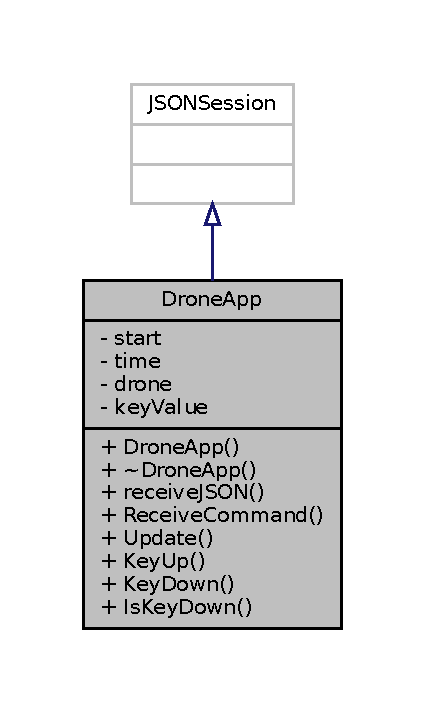
\includegraphics[width=204pt]{classDroneApp__inherit__graph}
\end{center}
\end{figure}


Collaboration diagram for Drone\+App\+:\nopagebreak
\begin{figure}[H]
\begin{center}
\leavevmode
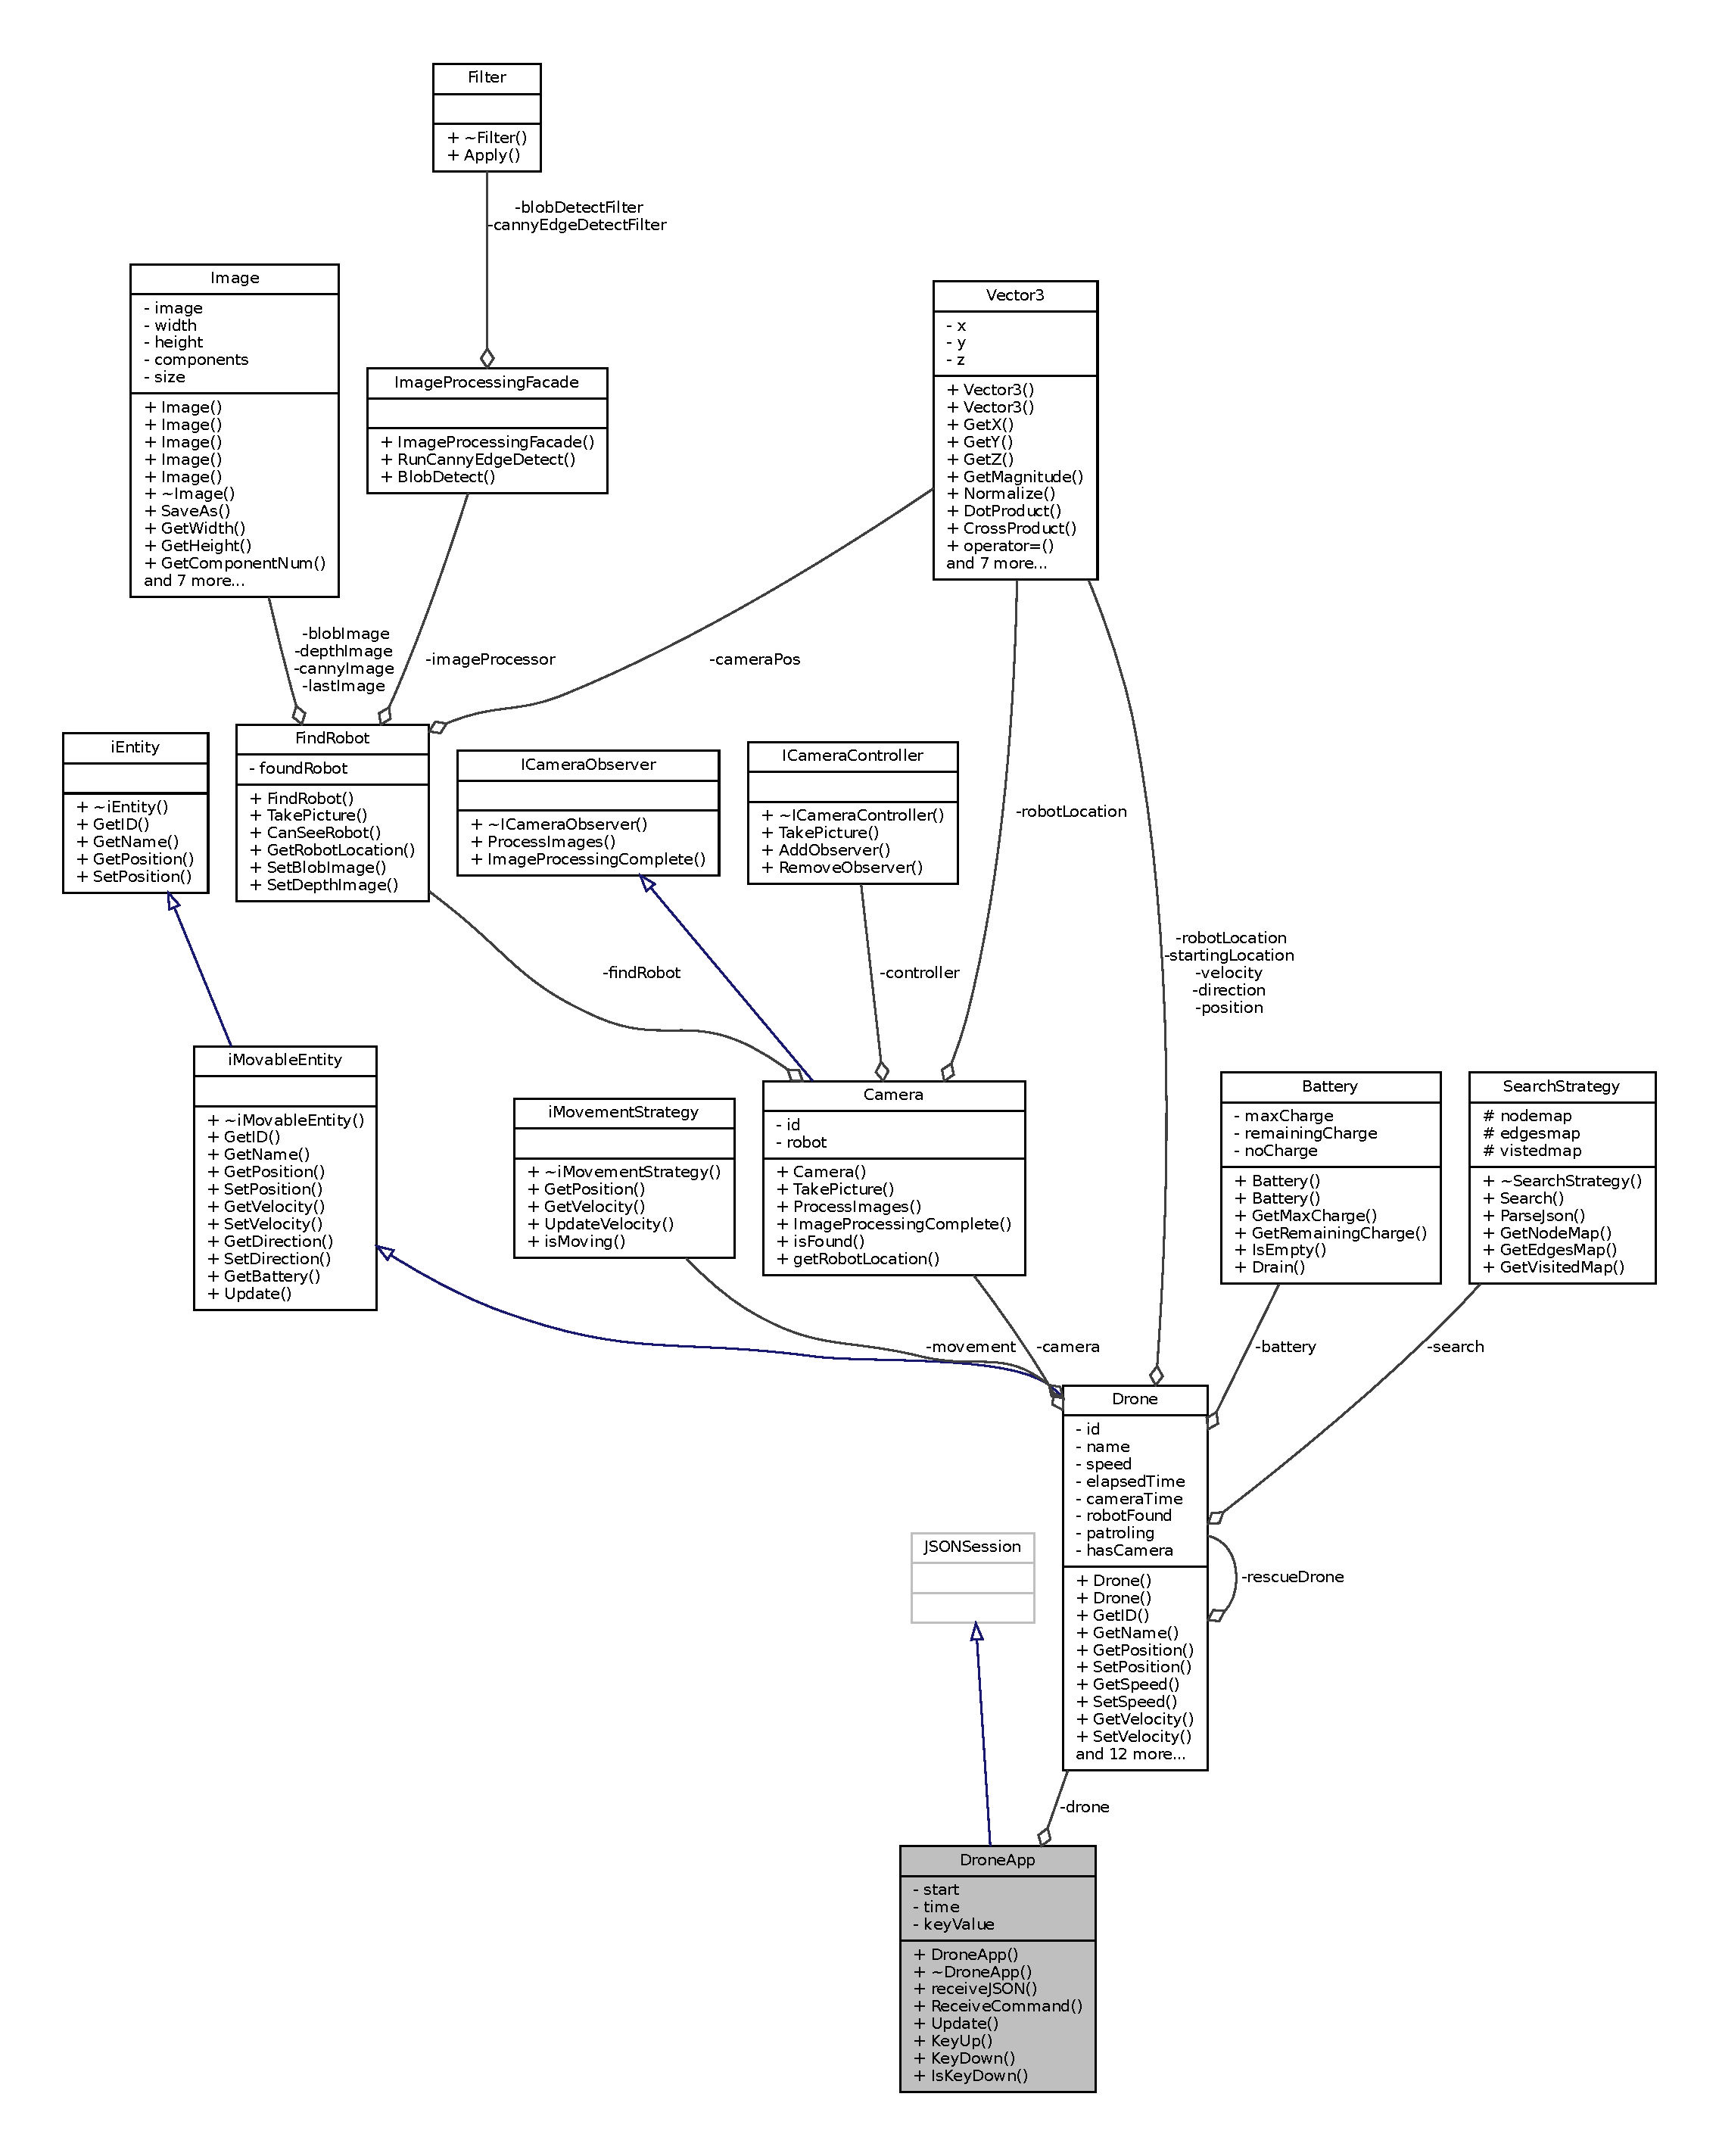
\includegraphics[width=350pt]{classDroneApp__coll__graph}
\end{center}
\end{figure}
\subsection*{Public Member Functions}
\begin{DoxyCompactItemize}
\item 
\mbox{\Hypertarget{classDroneApp_aee08991056bca317708c4600e9bafc9d}\label{classDroneApp_aee08991056bca317708c4600e9bafc9d}} 
void {\bfseries receive\+J\+S\+ON} (picojson\+::value \&val)
\item 
\mbox{\Hypertarget{classDroneApp_aadf6c66066f167d8bdbd0e4d69f16e31}\label{classDroneApp_aadf6c66066f167d8bdbd0e4d69f16e31}} 
void {\bfseries Receive\+Command} (const std\+::string \&cmd, picojson\+::object \&data, picojson\+::object \&return\+Value)
\item 
\mbox{\Hypertarget{classDroneApp_a9d9319844a7fe350933b7804c6972ab2}\label{classDroneApp_a9d9319844a7fe350933b7804c6972ab2}} 
void {\bfseries Update} (double dt, picojson\+::object \&return\+Value)
\item 
\mbox{\Hypertarget{classDroneApp_ac551dcfe12694ab624268469652ae2f9}\label{classDroneApp_ac551dcfe12694ab624268469652ae2f9}} 
void {\bfseries Key\+Up} (const std\+::string \&key, int key\+Code)
\item 
\mbox{\Hypertarget{classDroneApp_abd3255a9783ccfbc625bfa74a50238e9}\label{classDroneApp_abd3255a9783ccfbc625bfa74a50238e9}} 
void {\bfseries Key\+Down} (const std\+::string \&key, int key\+Code)
\item 
\mbox{\Hypertarget{classDroneApp_a9fa8bb8d0f5d5f9ca9042ca884f29181}\label{classDroneApp_a9fa8bb8d0f5d5f9ca9042ca884f29181}} 
bool {\bfseries Is\+Key\+Down} (const std\+::string \&key)
\end{DoxyCompactItemize}
\subsection*{Private Attributes}
\begin{DoxyCompactItemize}
\item 
\mbox{\Hypertarget{classDroneApp_a9c5deb39fbc163bab48cca209541cf9a}\label{classDroneApp_a9c5deb39fbc163bab48cca209541cf9a}} 
std\+::chrono\+::time\+\_\+point$<$ std\+::chrono\+::system\+\_\+clock $>$ {\bfseries start}
\item 
\mbox{\Hypertarget{classDroneApp_a83d0cd27e1a51dd509134dd4ac3f2f0a}\label{classDroneApp_a83d0cd27e1a51dd509134dd4ac3f2f0a}} 
double {\bfseries time}
\item 
\mbox{\Hypertarget{classDroneApp_ac92f3a39a20ebe12ceaac923c8f356d7}\label{classDroneApp_ac92f3a39a20ebe12ceaac923c8f356d7}} 
\hyperlink{classDrone}{Drone} {\bfseries drone}
\item 
\mbox{\Hypertarget{classDroneApp_a6023eb4a0c54568a36c754b7c0fc72e0}\label{classDroneApp_a6023eb4a0c54568a36c754b7c0fc72e0}} 
std\+::map$<$ std\+::string, int $>$ {\bfseries key\+Value}
\end{DoxyCompactItemize}


The documentation for this class was generated from the following file\+:\begin{DoxyCompactItemize}
\item 
/home/user/repo/project/simulation/include/drone\+\_\+app.\+h\end{DoxyCompactItemize}

\hypertarget{classDroneFactory}{}\section{Drone\+Factory Class Reference}
\label{classDroneFactory}\index{Drone\+Factory@{Drone\+Factory}}


\hyperlink{classDrone}{Drone} Factory. When called, it creates a new object of type \hyperlink{classDrone}{Drone}. This factory is never called directly, and is really only used through the composite entity factory.  




{\ttfamily \#include $<$drone\+\_\+factory.\+h$>$}



Inheritance diagram for Drone\+Factory\+:\nopagebreak
\begin{figure}[H]
\begin{center}
\leavevmode
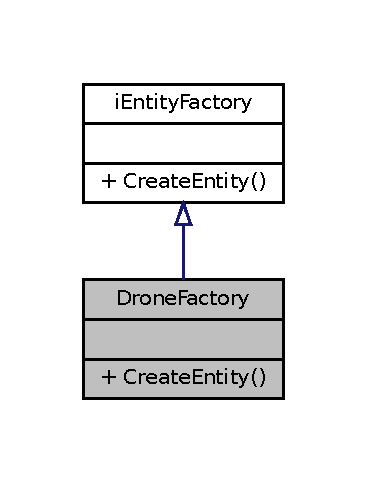
\includegraphics[width=176pt]{classDroneFactory__inherit__graph}
\end{center}
\end{figure}


Collaboration diagram for Drone\+Factory\+:\nopagebreak
\begin{figure}[H]
\begin{center}
\leavevmode
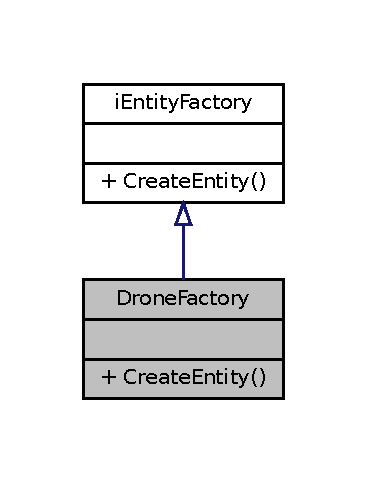
\includegraphics[width=176pt]{classDroneFactory__coll__graph}
\end{center}
\end{figure}
\subsection*{Public Member Functions}
\begin{DoxyCompactItemize}
\item 
\mbox{\Hypertarget{classDroneFactory_a9debaee3f504bd6506d7ddb9ebba0baf}\label{classDroneFactory_a9debaee3f504bd6506d7ddb9ebba0baf}} 
\hyperlink{classiEntity}{i\+Entity} $\ast$ \hyperlink{classDroneFactory_a9debaee3f504bd6506d7ddb9ebba0baf}{Create\+Entity} (picojson\+::object \&entity, \hyperlink{classCamera}{Camera} $\ast$camera)
\begin{DoxyCompactList}\small\item\em checks if type specified is drone. If so it creates and returns a pointer to our new drone object. But if the type doesn\textquotesingle{}t match, then it just returns a null pointer. \end{DoxyCompactList}\end{DoxyCompactItemize}


\subsection{Detailed Description}
\hyperlink{classDrone}{Drone} Factory. When called, it creates a new object of type \hyperlink{classDrone}{Drone}. This factory is never called directly, and is really only used through the composite entity factory. 

The documentation for this class was generated from the following files\+:\begin{DoxyCompactItemize}
\item 
/home/user/repo/project/simulation/include/\hyperlink{drone__factory_8h}{drone\+\_\+factory.\+h}\item 
/home/user/repo/project/simulation/src/drone\+\_\+factory.\+cc\end{DoxyCompactItemize}

\hypertarget{classFactoryTest}{}\section{Factory\+Test Class Reference}
\label{classFactoryTest}\index{Factory\+Test@{Factory\+Test}}


Integration tests for our composite factory pattern. These tests checks to see if our factory pattern correctly takes in picojson objects and converts them to an object\textquotesingle{}s member variables.  




Inheritance diagram for Factory\+Test\+:\nopagebreak
\begin{figure}[H]
\begin{center}
\leavevmode
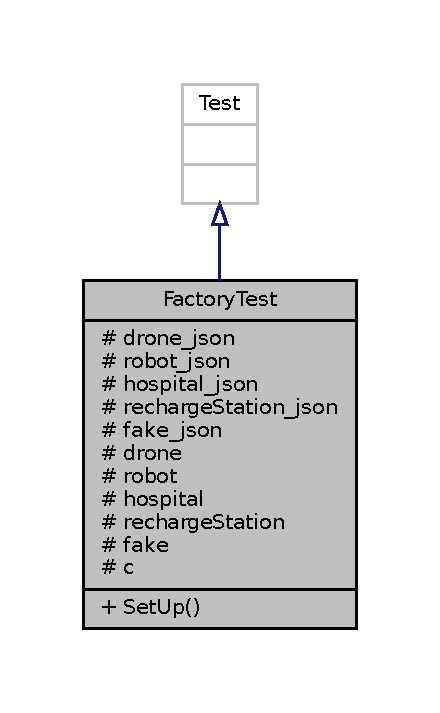
\includegraphics[width=211pt]{classFactoryTest__inherit__graph}
\end{center}
\end{figure}


Collaboration diagram for Factory\+Test\+:\nopagebreak
\begin{figure}[H]
\begin{center}
\leavevmode
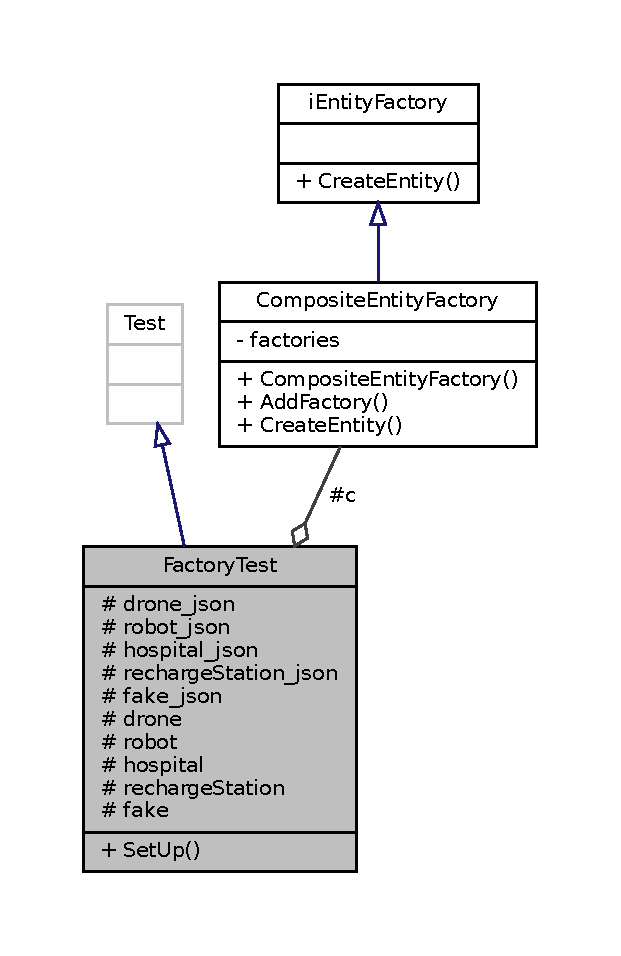
\includegraphics[width=298pt]{classFactoryTest__coll__graph}
\end{center}
\end{figure}
\subsection*{Public Member Functions}
\begin{DoxyCompactItemize}
\item 
\mbox{\Hypertarget{classFactoryTest_ab6472ece25a6c39a969974d839c4fbfe}\label{classFactoryTest_ab6472ece25a6c39a969974d839c4fbfe}} 
void \hyperlink{classFactoryTest_ab6472ece25a6c39a969974d839c4fbfe}{Set\+Up} ()
\begin{DoxyCompactList}\small\item\em Sets up our strings for the picojson parser to turn into picojson objects. One for each our our objects, and one string for a fake object to see if our factory can catch this. Also creates a composite entity factory to actually create our objects. \end{DoxyCompactList}\end{DoxyCompactItemize}
\subsection*{Protected Attributes}
\begin{DoxyCompactItemize}
\item 
\mbox{\Hypertarget{classFactoryTest_a79ee36408a3bd0b9e3832aef0faf4aa9}\label{classFactoryTest_a79ee36408a3bd0b9e3832aef0faf4aa9}} 
std\+::string \hyperlink{classFactoryTest_a79ee36408a3bd0b9e3832aef0faf4aa9}{drone\+\_\+json}
\begin{DoxyCompactList}\small\item\em strings to be parsed by picojson \end{DoxyCompactList}\item 
\mbox{\Hypertarget{classFactoryTest_a9aa8980ff0605062f20d1aa4930de3ee}\label{classFactoryTest_a9aa8980ff0605062f20d1aa4930de3ee}} 
std\+::string {\bfseries robot\+\_\+json}
\item 
\mbox{\Hypertarget{classFactoryTest_a083b566a58b74697cdb363be436282e9}\label{classFactoryTest_a083b566a58b74697cdb363be436282e9}} 
std\+::string {\bfseries hospital\+\_\+json}
\item 
\mbox{\Hypertarget{classFactoryTest_a6f96ef63a5f27273da007b8acf6653aa}\label{classFactoryTest_a6f96ef63a5f27273da007b8acf6653aa}} 
std\+::string {\bfseries recharge\+Station\+\_\+json}
\item 
\mbox{\Hypertarget{classFactoryTest_ab97fe3337f18068d9bac86868e140abc}\label{classFactoryTest_ab97fe3337f18068d9bac86868e140abc}} 
std\+::string {\bfseries fake\+\_\+json}
\item 
\mbox{\Hypertarget{classFactoryTest_ae385a634555c4972f9447b8524b1e3c4}\label{classFactoryTest_ae385a634555c4972f9447b8524b1e3c4}} 
picojson\+::value \hyperlink{classFactoryTest_ae385a634555c4972f9447b8524b1e3c4}{drone}
\begin{DoxyCompactList}\small\item\em picojson values representing data in their corresponding strings \end{DoxyCompactList}\item 
\mbox{\Hypertarget{classFactoryTest_a294af5fb898c91dbe57e39c9fb02c526}\label{classFactoryTest_a294af5fb898c91dbe57e39c9fb02c526}} 
picojson\+::value {\bfseries robot}
\item 
\mbox{\Hypertarget{classFactoryTest_aa9ccd66d84c4b78b2d8b40b8ed8fb047}\label{classFactoryTest_aa9ccd66d84c4b78b2d8b40b8ed8fb047}} 
picojson\+::value {\bfseries hospital}
\item 
\mbox{\Hypertarget{classFactoryTest_a2ff2744762c80740ffc28a26ebb7873f}\label{classFactoryTest_a2ff2744762c80740ffc28a26ebb7873f}} 
picojson\+::value {\bfseries recharge\+Station}
\item 
\mbox{\Hypertarget{classFactoryTest_aac81f20a5a2f99d7ffa57ce8e7bafebf}\label{classFactoryTest_aac81f20a5a2f99d7ffa57ce8e7bafebf}} 
picojson\+::value {\bfseries fake}
\item 
\mbox{\Hypertarget{classFactoryTest_aa34ecf518b28d27c6be3a16e705a1208}\label{classFactoryTest_aa34ecf518b28d27c6be3a16e705a1208}} 
\hyperlink{classCompositeEntityFactory}{Composite\+Entity\+Factory} \hyperlink{classFactoryTest_aa34ecf518b28d27c6be3a16e705a1208}{c}
\begin{DoxyCompactList}\small\item\em composite factory to actually create the objects used by our program \end{DoxyCompactList}\end{DoxyCompactItemize}


\subsection{Detailed Description}
Integration tests for our composite factory pattern. These tests checks to see if our factory pattern correctly takes in picojson objects and converts them to an object\textquotesingle{}s member variables. 

The documentation for this class was generated from the following file\+:\begin{DoxyCompactItemize}
\item 
/home/user/repo/project/tests/src/\hyperlink{factory__test_8cc}{factory\+\_\+test.\+cc}\end{DoxyCompactItemize}

\hypertarget{classFilter}{}\section{Filter Class Reference}
\label{classFilter}\index{Filter@{Filter}}


The main class for \hyperlink{classFilter}{Filter}. This is where all the filters are derived from.  




{\ttfamily \#include $<$filter.\+h$>$}



Inheritance diagram for Filter\+:\nopagebreak
\begin{figure}[H]
\begin{center}
\leavevmode
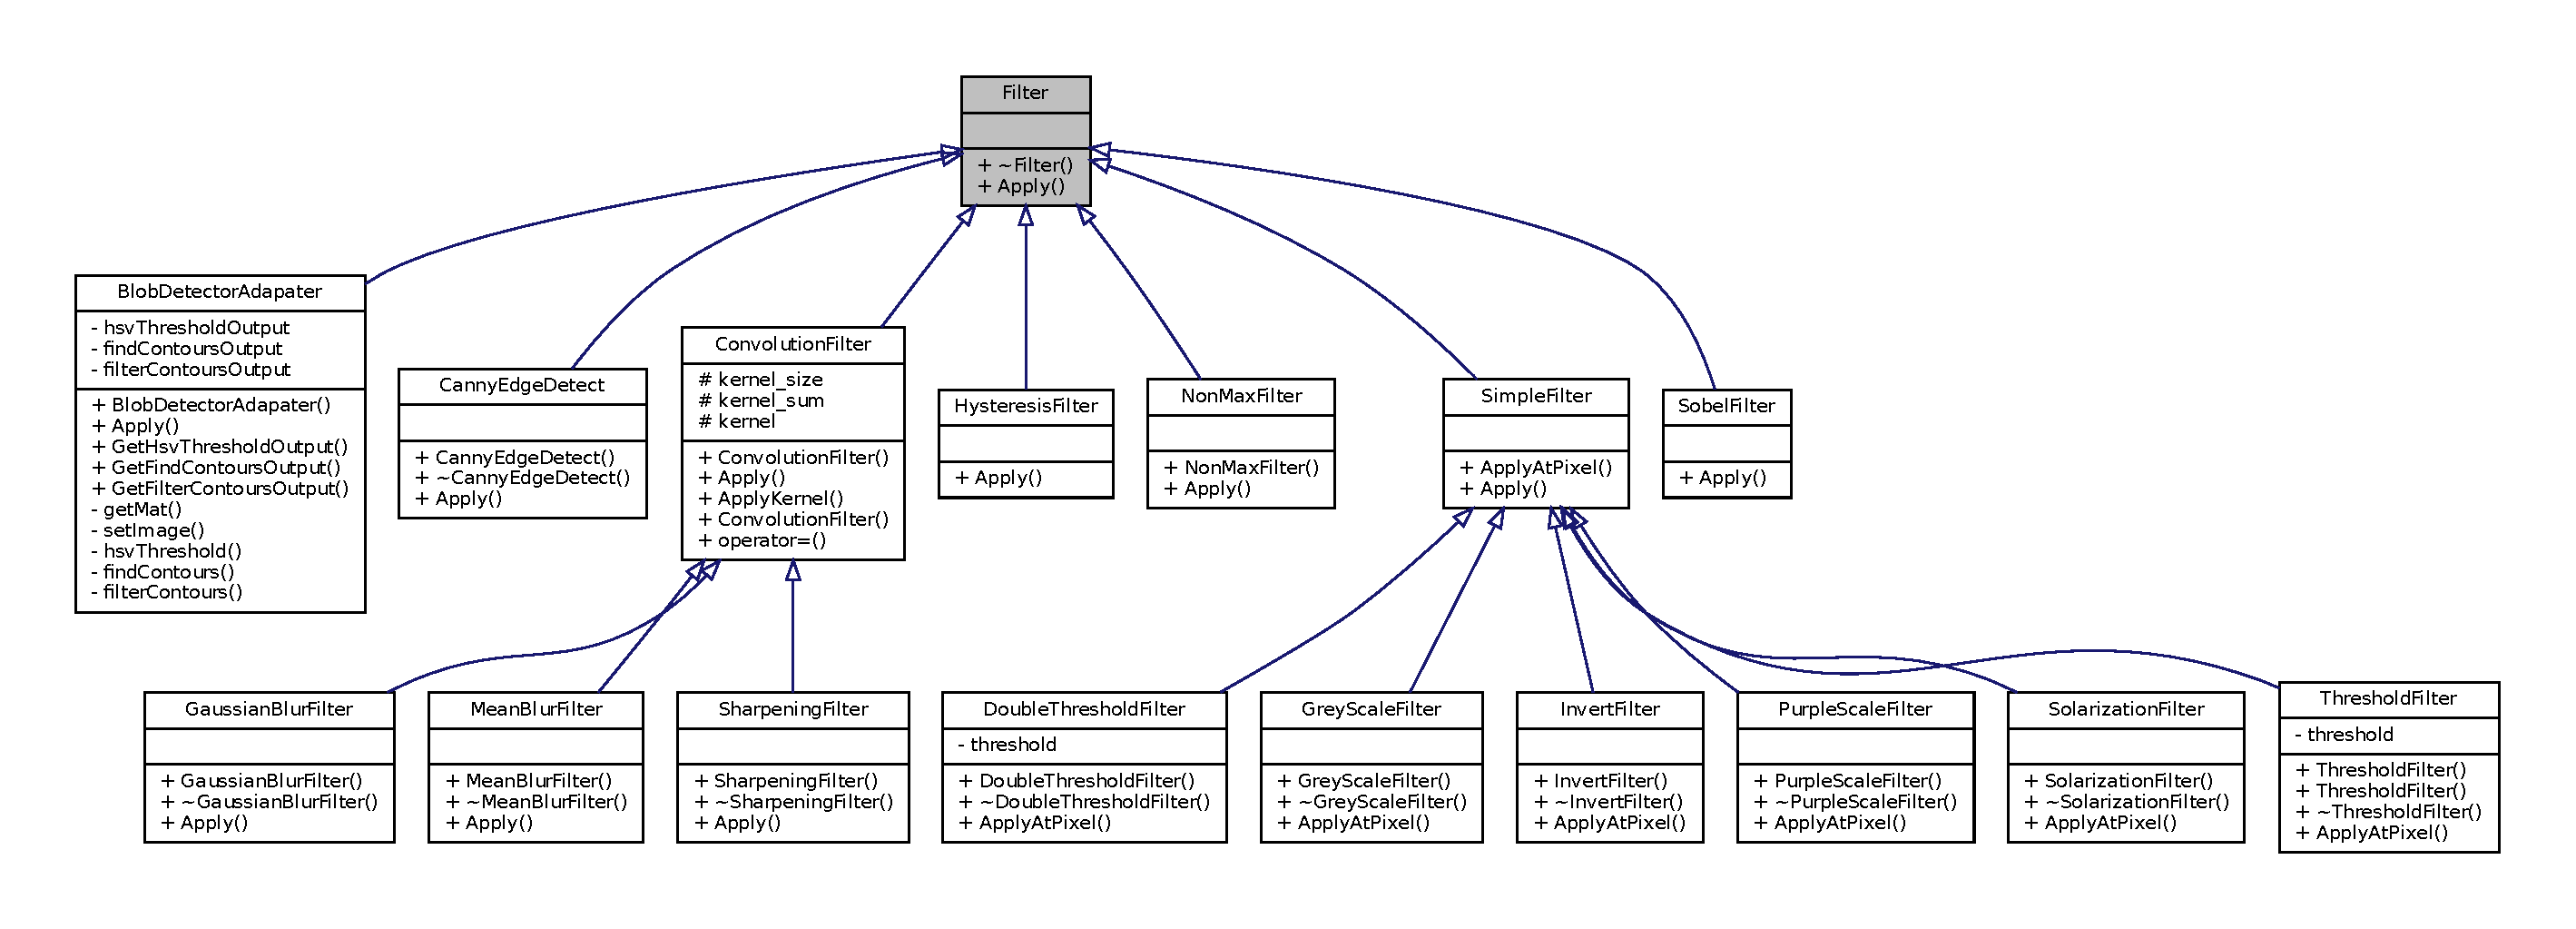
\includegraphics[width=350pt]{classFilter__inherit__graph}
\end{center}
\end{figure}


Collaboration diagram for Filter\+:\nopagebreak
\begin{figure}[H]
\begin{center}
\leavevmode
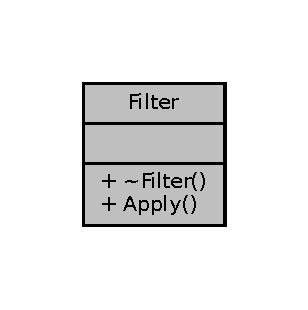
\includegraphics[width=148pt]{classFilter__coll__graph}
\end{center}
\end{figure}
\subsection*{Public Member Functions}
\begin{DoxyCompactItemize}
\item 
\mbox{\Hypertarget{classFilter_aa37dc017d133404b3a326f363ce36b8a}\label{classFilter_aa37dc017d133404b3a326f363ce36b8a}} 
virtual \hyperlink{classFilter_aa37dc017d133404b3a326f363ce36b8a}{$\sim$\+Filter} ()
\begin{DoxyCompactList}\small\item\em Destructor. \end{DoxyCompactList}\item 
\mbox{\Hypertarget{classFilter_afab0d50af44a19a370ebe46c69b8ff4e}\label{classFilter_afab0d50af44a19a370ebe46c69b8ff4e}} 
virtual void \hyperlink{classFilter_afab0d50af44a19a370ebe46c69b8ff4e}{Apply} (std\+::vector$<$ \hyperlink{classImage}{Image} $\ast$$>$ original, std\+::vector$<$ \hyperlink{classImage}{Image} $\ast$$>$ filtered)=0
\begin{DoxyCompactList}\small\item\em Apply function for filter (overrides most of the individual filters apply function) \end{DoxyCompactList}\end{DoxyCompactItemize}


\subsection{Detailed Description}
The main class for \hyperlink{classFilter}{Filter}. This is where all the filters are derived from. 

The documentation for this class was generated from the following file\+:\begin{DoxyCompactItemize}
\item 
/home/user/repo/project/image/include/\hyperlink{filter_8h}{filter.\+h}\end{DoxyCompactItemize}

\hypertarget{classFilterTest}{}\section{Filter\+Test Class Reference}
\label{classFilterTest}\index{Filter\+Test@{Filter\+Test}}


This is a series of unit tests to check how accurate my F\+FT image convolution filter works. In the image directory, there are a series of images with \char`\"{}expected\char`\"{} and \char`\"{}actual\char`\"{} suffixes. The expected comes from an online gaussian blur filter with size 13 kernel and an (i just guessed) standard deviation of 2. The site is \href{https://pinetools.com/blur-image}{\tt https\+://pinetools.\+com/blur-\/image}. The actual output comes from our image\+\_\+processor software, and I check to see how similar the pixel values are by summming up the differences and dividing by the size of the image.  




Inheritance diagram for Filter\+Test\+:\nopagebreak
\begin{figure}[H]
\begin{center}
\leavevmode
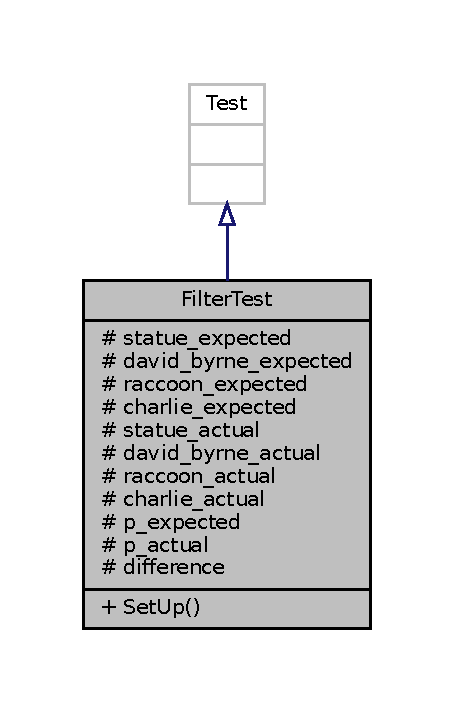
\includegraphics[width=218pt]{classFilterTest__inherit__graph}
\end{center}
\end{figure}


Collaboration diagram for Filter\+Test\+:\nopagebreak
\begin{figure}[H]
\begin{center}
\leavevmode
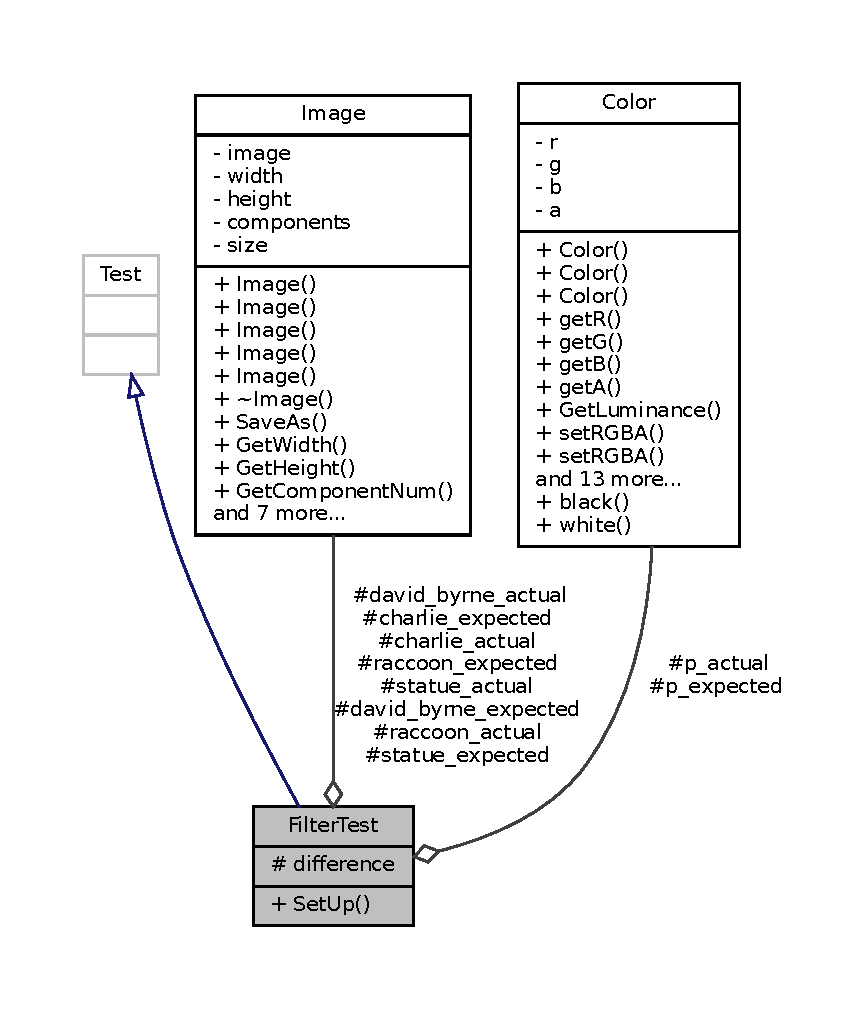
\includegraphics[width=350pt]{classFilterTest__coll__graph}
\end{center}
\end{figure}
\subsection*{Public Member Functions}
\begin{DoxyCompactItemize}
\item 
\mbox{\Hypertarget{classFilterTest_a567f17364b9c42da462b48570e518611}\label{classFilterTest_a567f17364b9c42da462b48570e518611}} 
void \hyperlink{classFilterTest_a567f17364b9c42da462b48570e518611}{Set\+Up} ()
\begin{DoxyCompactList}\small\item\em Initialize our images with our \hyperlink{classImage}{Image} class (which uses stbi image). This way we can have an array of color variables to make it easy to compare R\+GB values. Also have a double to calculate the difference of our image. The difference is summed up by every pixel and divided by the size of the image. Our actual tests check to see if the difference is below a threshold of. \end{DoxyCompactList}\end{DoxyCompactItemize}
\subsection*{Protected Attributes}
\begin{DoxyCompactItemize}
\item 
\mbox{\Hypertarget{classFilterTest_a7e7482ea23023c3202bb9e5609d9413b}\label{classFilterTest_a7e7482ea23023c3202bb9e5609d9413b}} 
\hyperlink{classImage}{Image} {\bfseries statue\+\_\+expected}
\item 
\mbox{\Hypertarget{classFilterTest_a81be93944fe9f57974da5c8bb6ac3617}\label{classFilterTest_a81be93944fe9f57974da5c8bb6ac3617}} 
\hyperlink{classImage}{Image} {\bfseries david\+\_\+byrne\+\_\+expected}
\item 
\mbox{\Hypertarget{classFilterTest_a7273edc926ab2971cfc9e12e2b9d6555}\label{classFilterTest_a7273edc926ab2971cfc9e12e2b9d6555}} 
\hyperlink{classImage}{Image} {\bfseries raccoon\+\_\+expected}
\item 
\mbox{\Hypertarget{classFilterTest_a3ef4a77ef46f52da74322edf24faeed0}\label{classFilterTest_a3ef4a77ef46f52da74322edf24faeed0}} 
\hyperlink{classImage}{Image} {\bfseries charlie\+\_\+expected}
\item 
\mbox{\Hypertarget{classFilterTest_a09439a0fc55b7f5e4eb515951999bfe4}\label{classFilterTest_a09439a0fc55b7f5e4eb515951999bfe4}} 
\hyperlink{classImage}{Image} {\bfseries statue\+\_\+actual}
\item 
\mbox{\Hypertarget{classFilterTest_a1f0639bf0a6e95d3a5eeb8977ba205ee}\label{classFilterTest_a1f0639bf0a6e95d3a5eeb8977ba205ee}} 
\hyperlink{classImage}{Image} {\bfseries david\+\_\+byrne\+\_\+actual}
\item 
\mbox{\Hypertarget{classFilterTest_a076aa20d78baf77c030ee5add68fb30c}\label{classFilterTest_a076aa20d78baf77c030ee5add68fb30c}} 
\hyperlink{classImage}{Image} {\bfseries raccoon\+\_\+actual}
\item 
\mbox{\Hypertarget{classFilterTest_a7058570c48eb0366c64432ea2f57cd3e}\label{classFilterTest_a7058570c48eb0366c64432ea2f57cd3e}} 
\hyperlink{classImage}{Image} {\bfseries charlie\+\_\+actual}
\item 
\mbox{\Hypertarget{classFilterTest_a3cb5dd86460cee60ba6b3151c1d22bc6}\label{classFilterTest_a3cb5dd86460cee60ba6b3151c1d22bc6}} 
\hyperlink{classColor}{Color} {\bfseries p\+\_\+expected}
\item 
\mbox{\Hypertarget{classFilterTest_a84d38a7b7bc094940ae6cb0eb85b2568}\label{classFilterTest_a84d38a7b7bc094940ae6cb0eb85b2568}} 
\hyperlink{classColor}{Color} {\bfseries p\+\_\+actual}
\item 
\mbox{\Hypertarget{classFilterTest_a911c09fcff3001d56005f8e1cea98125}\label{classFilterTest_a911c09fcff3001d56005f8e1cea98125}} 
double {\bfseries difference}
\end{DoxyCompactItemize}


\subsection{Detailed Description}
This is a series of unit tests to check how accurate my F\+FT image convolution filter works. In the image directory, there are a series of images with \char`\"{}expected\char`\"{} and \char`\"{}actual\char`\"{} suffixes. The expected comes from an online gaussian blur filter with size 13 kernel and an (i just guessed) standard deviation of 2. The site is \href{https://pinetools.com/blur-image}{\tt https\+://pinetools.\+com/blur-\/image}. The actual output comes from our image\+\_\+processor software, and I check to see how similar the pixel values are by summming up the differences and dividing by the size of the image. 

The documentation for this class was generated from the following file\+:\begin{DoxyCompactItemize}
\item 
/home/user/repo/project/tests/src/\hyperlink{fft__convolution__test_8cc}{fft\+\_\+convolution\+\_\+test.\+cc}\end{DoxyCompactItemize}

\hypertarget{classFindRobot}{}\section{Find\+Robot Class Reference}
\label{classFindRobot}\index{Find\+Robot@{Find\+Robot}}


This class takes in an image and using the image processing facade runs the logic on images to see if the robot is found.  




{\ttfamily \#include $<$find\+\_\+robot.\+h$>$}



Collaboration diagram for Find\+Robot\+:\nopagebreak
\begin{figure}[H]
\begin{center}
\leavevmode
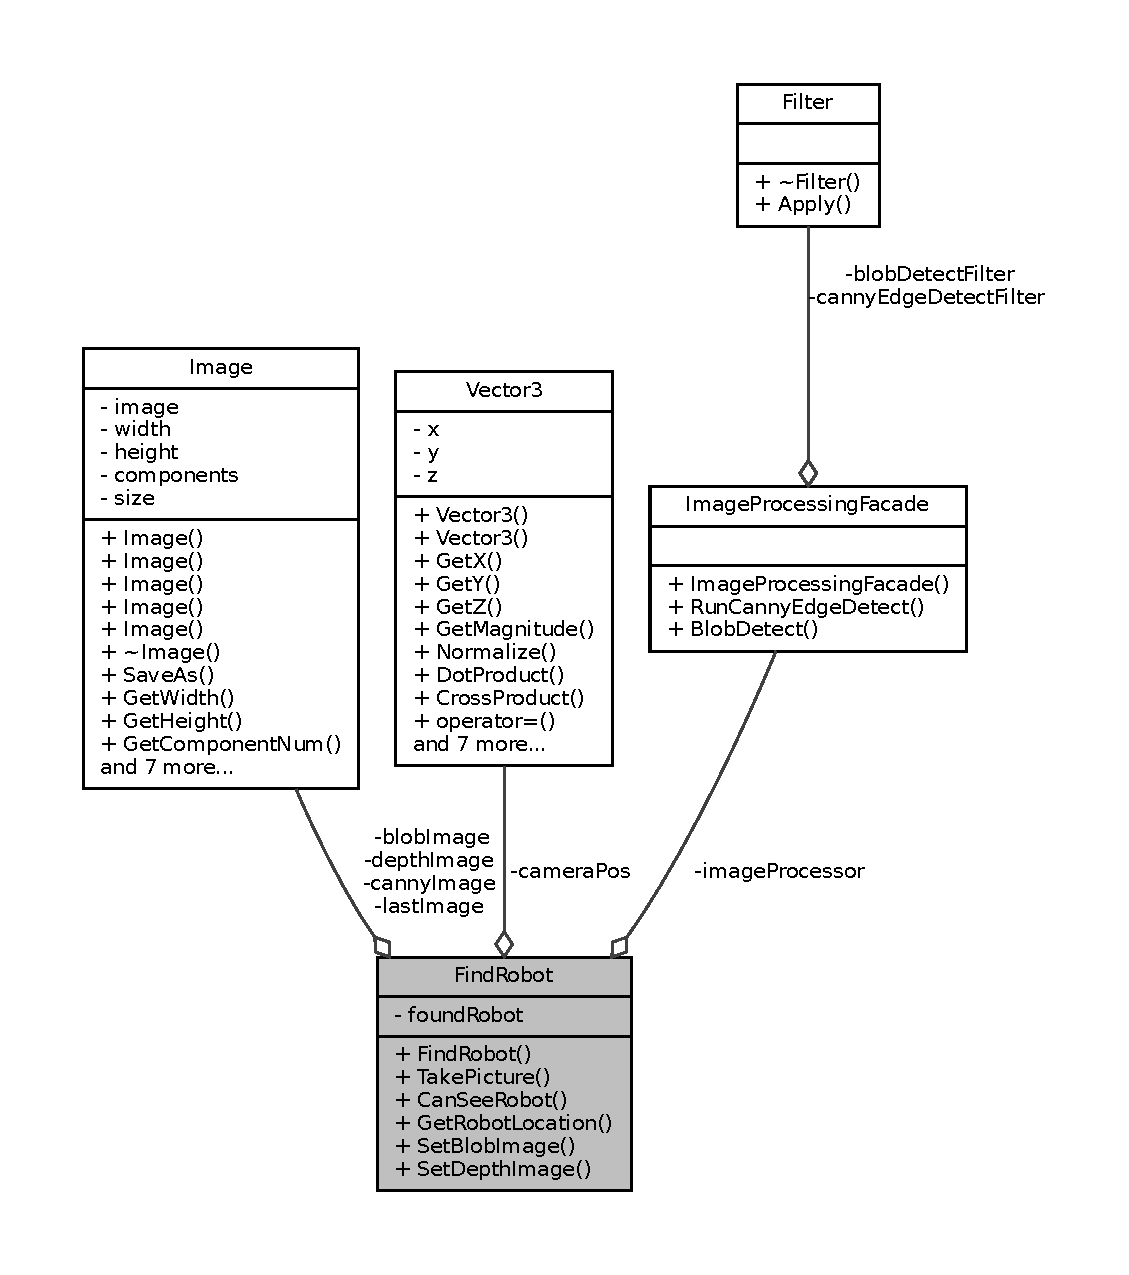
\includegraphics[width=350pt]{classFindRobot__coll__graph}
\end{center}
\end{figure}
\subsection*{Public Member Functions}
\begin{DoxyCompactItemize}
\item 
\mbox{\Hypertarget{classFindRobot_a55011d75f3703849bf1e8bd49ea72a4c}\label{classFindRobot_a55011d75f3703849bf1e8bd49ea72a4c}} 
\hyperlink{classFindRobot_a55011d75f3703849bf1e8bd49ea72a4c}{Find\+Robot} ()
\begin{DoxyCompactList}\small\item\em Construct a new Find \hyperlink{classRobot}{Robot} object. \end{DoxyCompactList}\item 
void \hyperlink{classFindRobot_a27fed71d7793129a281fc7a3174d328b}{Take\+Picture} (\hyperlink{classVector3}{Vector3} $\ast$camera\+Position, \hyperlink{classImage}{Image} $\ast$rgb, \hyperlink{classImage}{Image} $\ast$depth)
\begin{DoxyCompactList}\small\item\em Receives and image from the simulation, and runs the image processing facade on them. \end{DoxyCompactList}\item 
bool \hyperlink{classFindRobot_ae26378cc41e2e3c61e4833ec0e7b1d76}{Can\+See\+Robot} (int \&outX, int \&outY)
\begin{DoxyCompactList}\small\item\em This is the function that does all the logic work, it takes the processesd images and returns true of false if the robot is inside the images. It then returns the X and Y coordinates of where the robot is in the image. This information is stored in the top left pixel of the blob image. The format is ($<$1 or 0, can see$>$, $<$robot x$>$=\char`\"{}\char`\"{}$>$, $<$robot y$>$=\char`\"{}\char`\"{}$>$). \end{DoxyCompactList}\item 
\hyperlink{classVector3}{Vector3} \hyperlink{classFindRobot_acab7123d6f276e150b87ea30f1f287d4}{Get\+Robot\+Location} (int x, int y)
\begin{DoxyCompactList}\small\item\em Get the \hyperlink{classRobot}{Robot} Location object, from the X and Y coordinates from Can\+See\+Robot. This function requires the depth image be updated. \end{DoxyCompactList}\item 
\mbox{\Hypertarget{classFindRobot_a63e77c7b9a876332fc3fb411bb6644a9}\label{classFindRobot_a63e77c7b9a876332fc3fb411bb6644a9}} 
void \hyperlink{classFindRobot_a63e77c7b9a876332fc3fb411bb6644a9}{Set\+Blob\+Image} (\hyperlink{classImage}{Image} $\ast$blob)
\begin{DoxyCompactList}\small\item\em Sets the blob image. \end{DoxyCompactList}\item 
\mbox{\Hypertarget{classFindRobot_a1aac26d16ab0e8ffc3fd1c587b96991e}\label{classFindRobot_a1aac26d16ab0e8ffc3fd1c587b96991e}} 
void \hyperlink{classFindRobot_a1aac26d16ab0e8ffc3fd1c587b96991e}{Set\+Depth\+Image} (\hyperlink{classImage}{Image} $\ast$depth)
\begin{DoxyCompactList}\small\item\em Sets the depth image. \end{DoxyCompactList}\end{DoxyCompactItemize}
\subsection*{Private Attributes}
\begin{DoxyCompactItemize}
\item 
\mbox{\Hypertarget{classFindRobot_a009faddfec003a049608fb535521c09f}\label{classFindRobot_a009faddfec003a049608fb535521c09f}} 
\hyperlink{classImageProcessingFacade}{Image\+Processing\+Facade} $\ast$ \hyperlink{classFindRobot_a009faddfec003a049608fb535521c09f}{image\+Processor}
\begin{DoxyCompactList}\small\item\em The image processing facade class. \end{DoxyCompactList}\item 
\mbox{\Hypertarget{classFindRobot_a68e82ba1b2ef89dd1a767e917b70bf2a}\label{classFindRobot_a68e82ba1b2ef89dd1a767e917b70bf2a}} 
\hyperlink{classVector3}{Vector3} \hyperlink{classFindRobot_a68e82ba1b2ef89dd1a767e917b70bf2a}{camera\+Pos}
\begin{DoxyCompactList}\small\item\em The position of the camera when the images were taken. \end{DoxyCompactList}\item 
\mbox{\Hypertarget{classFindRobot_a1c53be1c0b13581f8fe833090776cc21}\label{classFindRobot_a1c53be1c0b13581f8fe833090776cc21}} 
\hyperlink{classImage}{Image} $\ast$ \hyperlink{classFindRobot_a1c53be1c0b13581f8fe833090776cc21}{last\+Image}
\begin{DoxyCompactList}\small\item\em The last rgb image taken from the camera. \end{DoxyCompactList}\item 
\mbox{\Hypertarget{classFindRobot_a8560b99cd1110bb459af3d862b3695a3}\label{classFindRobot_a8560b99cd1110bb459af3d862b3695a3}} 
\hyperlink{classImage}{Image} $\ast$ \hyperlink{classFindRobot_a8560b99cd1110bb459af3d862b3695a3}{depth\+Image}
\begin{DoxyCompactList}\small\item\em The last depth image taken from the camera. \end{DoxyCompactList}\item 
\mbox{\Hypertarget{classFindRobot_ab57facf1a4ca4ae4a52c088d45949a41}\label{classFindRobot_ab57facf1a4ca4ae4a52c088d45949a41}} 
\hyperlink{classImage}{Image} $\ast$ \hyperlink{classFindRobot_ab57facf1a4ca4ae4a52c088d45949a41}{blob\+Image}
\begin{DoxyCompactList}\small\item\em This is the blob image from Open\+CV. \end{DoxyCompactList}\item 
\mbox{\Hypertarget{classFindRobot_ae5bfaf2d47f0db2af41661a3d844fa4a}\label{classFindRobot_ae5bfaf2d47f0db2af41661a3d844fa4a}} 
\hyperlink{classImage}{Image} $\ast$ \hyperlink{classFindRobot_ae5bfaf2d47f0db2af41661a3d844fa4a}{canny\+Image}
\begin{DoxyCompactList}\small\item\em This is the canny edge detect image from Image\+Processor. \end{DoxyCompactList}\item 
\mbox{\Hypertarget{classFindRobot_aee4ed8c42df1924a51014976dcc6ac7a}\label{classFindRobot_aee4ed8c42df1924a51014976dcc6ac7a}} 
bool \hyperlink{classFindRobot_aee4ed8c42df1924a51014976dcc6ac7a}{found\+Robot} = false
\begin{DoxyCompactList}\small\item\em Is the robot found. \end{DoxyCompactList}\end{DoxyCompactItemize}


\subsection{Detailed Description}
This class takes in an image and using the image processing facade runs the logic on images to see if the robot is found. 

\subsection{Member Function Documentation}
\mbox{\Hypertarget{classFindRobot_ae26378cc41e2e3c61e4833ec0e7b1d76}\label{classFindRobot_ae26378cc41e2e3c61e4833ec0e7b1d76}} 
\index{Find\+Robot@{Find\+Robot}!Can\+See\+Robot@{Can\+See\+Robot}}
\index{Can\+See\+Robot@{Can\+See\+Robot}!Find\+Robot@{Find\+Robot}}
\subsubsection{\texorpdfstring{Can\+See\+Robot()}{CanSeeRobot()}}
{\footnotesize\ttfamily bool Find\+Robot\+::\+Can\+See\+Robot (\begin{DoxyParamCaption}\item[{int \&}]{outX,  }\item[{int \&}]{outY }\end{DoxyParamCaption})\hspace{0.3cm}{\ttfamily [inline]}}



This is the function that does all the logic work, it takes the processesd images and returns true of false if the robot is inside the images. It then returns the X and Y coordinates of where the robot is in the image. This information is stored in the top left pixel of the blob image. The format is ($<$1 or 0, can see$>$, $<$robot x$>$=\char`\"{}\char`\"{}$>$, $<$robot y$>$=\char`\"{}\char`\"{}$>$). 


\begin{DoxyParams}{Parameters}
{\em outX} & \\
\hline
{\em outY} & \\
\hline
\end{DoxyParams}
\begin{DoxyReturn}{Returns}
true 

false 
\end{DoxyReturn}
\mbox{\Hypertarget{classFindRobot_acab7123d6f276e150b87ea30f1f287d4}\label{classFindRobot_acab7123d6f276e150b87ea30f1f287d4}} 
\index{Find\+Robot@{Find\+Robot}!Get\+Robot\+Location@{Get\+Robot\+Location}}
\index{Get\+Robot\+Location@{Get\+Robot\+Location}!Find\+Robot@{Find\+Robot}}
\subsubsection{\texorpdfstring{Get\+Robot\+Location()}{GetRobotLocation()}}
{\footnotesize\ttfamily \hyperlink{classVector3}{Vector3} Find\+Robot\+::\+Get\+Robot\+Location (\begin{DoxyParamCaption}\item[{int}]{x,  }\item[{int}]{y }\end{DoxyParamCaption})\hspace{0.3cm}{\ttfamily [inline]}}



Get the \hyperlink{classRobot}{Robot} Location object, from the X and Y coordinates from Can\+See\+Robot. This function requires the depth image be updated. 


\begin{DoxyParams}{Parameters}
{\em x} & \\
\hline
{\em y} & \\
\hline
\end{DoxyParams}
\begin{DoxyReturn}{Returns}
\hyperlink{classVector3}{Vector3} 
\end{DoxyReturn}
\mbox{\Hypertarget{classFindRobot_a27fed71d7793129a281fc7a3174d328b}\label{classFindRobot_a27fed71d7793129a281fc7a3174d328b}} 
\index{Find\+Robot@{Find\+Robot}!Take\+Picture@{Take\+Picture}}
\index{Take\+Picture@{Take\+Picture}!Find\+Robot@{Find\+Robot}}
\subsubsection{\texorpdfstring{Take\+Picture()}{TakePicture()}}
{\footnotesize\ttfamily void Find\+Robot\+::\+Take\+Picture (\begin{DoxyParamCaption}\item[{\hyperlink{classVector3}{Vector3} $\ast$}]{camera\+Position,  }\item[{\hyperlink{classImage}{Image} $\ast$}]{rgb,  }\item[{\hyperlink{classImage}{Image} $\ast$}]{depth }\end{DoxyParamCaption})\hspace{0.3cm}{\ttfamily [inline]}}



Receives and image from the simulation, and runs the image processing facade on them. 


\begin{DoxyParams}{Parameters}
{\em camera\+Position} & \\
\hline
{\em rgb} & \\
\hline
{\em depth} & \\
\hline
\end{DoxyParams}


The documentation for this class was generated from the following file\+:\begin{DoxyCompactItemize}
\item 
/home/user/repo/project/simulation/include/\hyperlink{find__robot_8h}{find\+\_\+robot.\+h}\end{DoxyCompactItemize}

\hypertarget{classFindRobotTest}{}\section{Find\+Robot\+Test Class Reference}
\label{classFindRobotTest}\index{Find\+Robot\+Test@{Find\+Robot\+Test}}


Inheritance diagram for Find\+Robot\+Test\+:\nopagebreak
\begin{figure}[H]
\begin{center}
\leavevmode
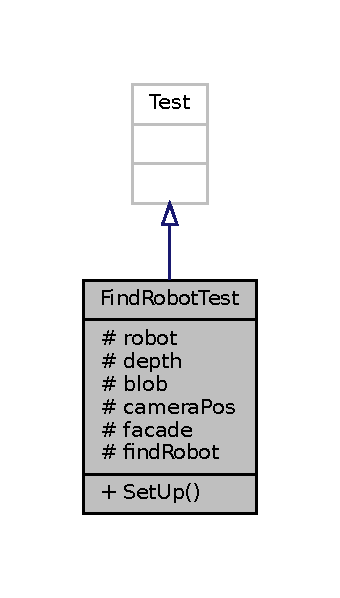
\includegraphics[width=163pt]{classFindRobotTest__inherit__graph}
\end{center}
\end{figure}


Collaboration diagram for Find\+Robot\+Test\+:\nopagebreak
\begin{figure}[H]
\begin{center}
\leavevmode
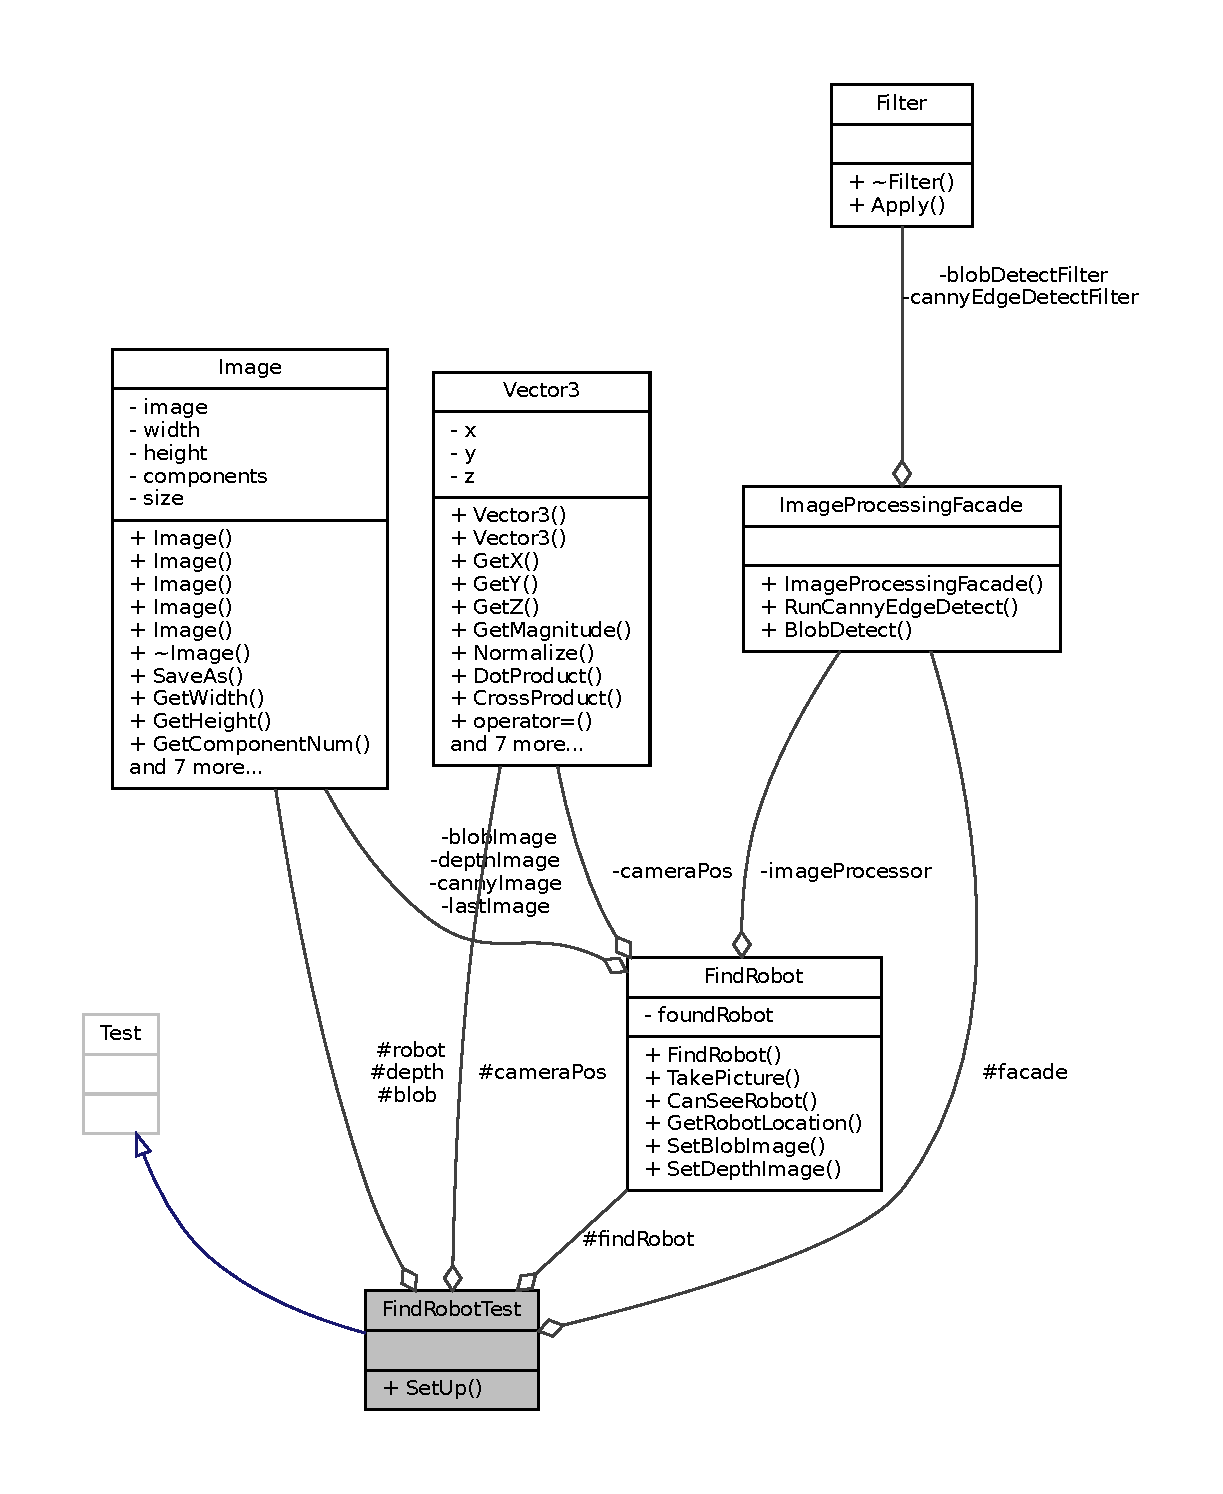
\includegraphics[width=350pt]{classFindRobotTest__coll__graph}
\end{center}
\end{figure}
\subsection*{Public Member Functions}
\begin{DoxyCompactItemize}
\item 
\mbox{\Hypertarget{classFindRobotTest_a69c8326a85f9f30b918555197160c29a}\label{classFindRobotTest_a69c8326a85f9f30b918555197160c29a}} 
void {\bfseries Set\+Up} ()
\end{DoxyCompactItemize}
\subsection*{Protected Attributes}
\begin{DoxyCompactItemize}
\item 
\mbox{\Hypertarget{classFindRobotTest_a9a744772cdef7072a8bbab420ef65fa4}\label{classFindRobotTest_a9a744772cdef7072a8bbab420ef65fa4}} 
\hyperlink{classImage}{Image} $\ast$ {\bfseries robot}
\item 
\mbox{\Hypertarget{classFindRobotTest_a8bf80cbf9f44ca61c1d0da2158e6a621}\label{classFindRobotTest_a8bf80cbf9f44ca61c1d0da2158e6a621}} 
\hyperlink{classImage}{Image} $\ast$ {\bfseries depth}
\item 
\mbox{\Hypertarget{classFindRobotTest_a46c821bad76c3f27b89383e3c7ca0899}\label{classFindRobotTest_a46c821bad76c3f27b89383e3c7ca0899}} 
\hyperlink{classImage}{Image} $\ast$ {\bfseries blob}
\item 
\mbox{\Hypertarget{classFindRobotTest_a374a454baef6f6983f892196abc9bc5c}\label{classFindRobotTest_a374a454baef6f6983f892196abc9bc5c}} 
\hyperlink{classVector3}{Vector3} {\bfseries camera\+Pos}
\item 
\mbox{\Hypertarget{classFindRobotTest_a90dad3e688d09c1cb5815caa691fd511}\label{classFindRobotTest_a90dad3e688d09c1cb5815caa691fd511}} 
\hyperlink{classImageProcessingFacade}{Image\+Processing\+Facade} {\bfseries facade}
\item 
\mbox{\Hypertarget{classFindRobotTest_ae38d4635ebab2e64fc1c880f39350184}\label{classFindRobotTest_ae38d4635ebab2e64fc1c880f39350184}} 
\hyperlink{classFindRobot}{Find\+Robot} {\bfseries find\+Robot}
\end{DoxyCompactItemize}


The documentation for this class was generated from the following file\+:\begin{DoxyCompactItemize}
\item 
/home/user/repo/project/tests/src/find\+\_\+robot\+\_\+test.\+cc\end{DoxyCompactItemize}

\hypertarget{classGaussianBlurFilter}{}\section{Gaussian\+Blur\+Filter Class Reference}
\label{classGaussianBlurFilter}\index{Gaussian\+Blur\+Filter@{Gaussian\+Blur\+Filter}}


The main class for \hyperlink{classGaussianBlurFilter}{Gaussian\+Blur\+Filter}, extends \hyperlink{classConvolutionFilter}{Convolution\+Filter}. Creates a 5 x 5 kernel to apply to each pixel and \hyperlink{classConvolutionFilter}{Convolution\+Filter} is used to iterate through the image to apply it. Gaussian Blur is different from Mean Blur in that the representation of each pixel isn\textquotesingle{}t equally distributed like Mean Blur.  




{\ttfamily \#include $<$gaussian\+\_\+blur\+\_\+filter.\+h$>$}



Inheritance diagram for Gaussian\+Blur\+Filter\+:\nopagebreak
\begin{figure}[H]
\begin{center}
\leavevmode
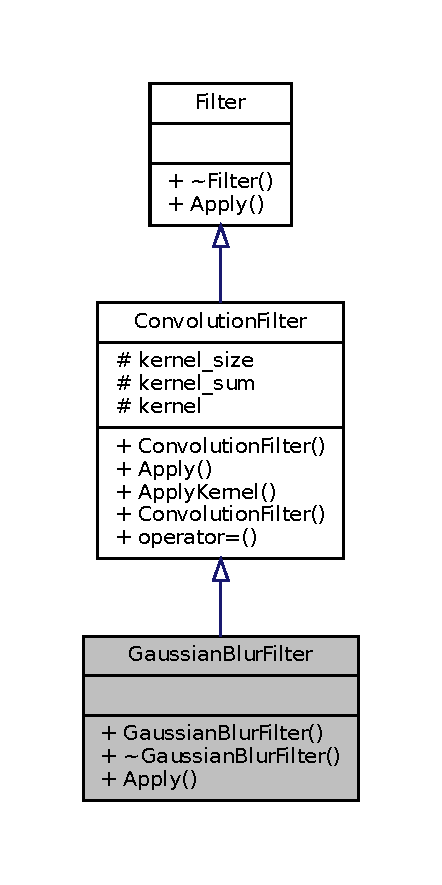
\includegraphics[width=212pt]{classGaussianBlurFilter__inherit__graph}
\end{center}
\end{figure}


Collaboration diagram for Gaussian\+Blur\+Filter\+:\nopagebreak
\begin{figure}[H]
\begin{center}
\leavevmode
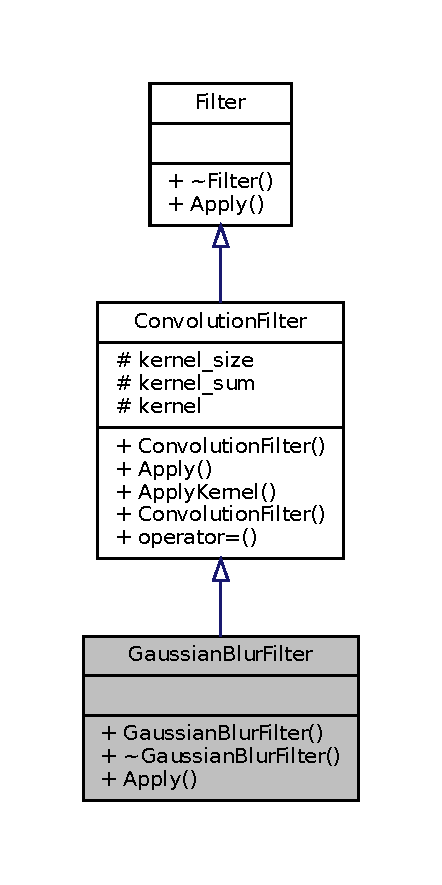
\includegraphics[width=212pt]{classGaussianBlurFilter__coll__graph}
\end{center}
\end{figure}
\subsection*{Public Member Functions}
\begin{DoxyCompactItemize}
\item 
\mbox{\Hypertarget{classGaussianBlurFilter_a5b073291df50d87077650371c90af0f9}\label{classGaussianBlurFilter_a5b073291df50d87077650371c90af0f9}} 
\hyperlink{classGaussianBlurFilter_a5b073291df50d87077650371c90af0f9}{Gaussian\+Blur\+Filter} ()
\begin{DoxyCompactList}\small\item\em Constructor. \end{DoxyCompactList}\item 
\mbox{\Hypertarget{classGaussianBlurFilter_a371400ed538c678311cc950f8eaa5218}\label{classGaussianBlurFilter_a371400ed538c678311cc950f8eaa5218}} 
\hyperlink{classGaussianBlurFilter_a371400ed538c678311cc950f8eaa5218}{$\sim$\+Gaussian\+Blur\+Filter} ()
\begin{DoxyCompactList}\small\item\em Constructor. \end{DoxyCompactList}\item 
\mbox{\Hypertarget{classGaussianBlurFilter_a8260deac8ea6cda8e473bc6da0846bff}\label{classGaussianBlurFilter_a8260deac8ea6cda8e473bc6da0846bff}} 
void \hyperlink{classGaussianBlurFilter_a8260deac8ea6cda8e473bc6da0846bff}{Apply} (std\+::vector$<$ \hyperlink{classImage}{Image} $\ast$$>$ original, std\+::vector$<$ \hyperlink{classImage}{Image} $\ast$$>$ filtered)
\begin{DoxyCompactList}\small\item\em Apply function to be overridden by parents Apply function. \end{DoxyCompactList}\end{DoxyCompactItemize}
\subsection*{Additional Inherited Members}


\subsection{Detailed Description}
The main class for \hyperlink{classGaussianBlurFilter}{Gaussian\+Blur\+Filter}, extends \hyperlink{classConvolutionFilter}{Convolution\+Filter}. Creates a 5 x 5 kernel to apply to each pixel and \hyperlink{classConvolutionFilter}{Convolution\+Filter} is used to iterate through the image to apply it. Gaussian Blur is different from Mean Blur in that the representation of each pixel isn\textquotesingle{}t equally distributed like Mean Blur. 

The documentation for this class was generated from the following files\+:\begin{DoxyCompactItemize}
\item 
/home/user/repo/project/image/include/\hyperlink{gaussian__blur__filter_8h}{gaussian\+\_\+blur\+\_\+filter.\+h}\item 
/home/user/repo/project/image/src/gaussian\+\_\+blur\+\_\+filter.\+cc\end{DoxyCompactItemize}

\hypertarget{classGreyScaleFilter}{}\section{Grey\+Scale\+Filter Class Reference}
\label{classGreyScaleFilter}\index{Grey\+Scale\+Filter@{Grey\+Scale\+Filter}}


The main class for \hyperlink{classGreyScaleFilter}{Grey\+Scale\+Filter}, extends \hyperlink{classSimpleFilter}{Simple\+Filter}. Overrides the virtual \hyperlink{classGreyScaleFilter_ac781a1ddd205f2d67d1c08481d5ab2e4}{Apply\+At\+Pixel()} function defined in \hyperlink{classSimpleFilter}{Simple\+Filter}. Just calculates the luminance value of each pixel and sets the pixels rgb values to the luminance.  




{\ttfamily \#include $<$greyscale\+\_\+filter.\+h$>$}



Inheritance diagram for Grey\+Scale\+Filter\+:\nopagebreak
\begin{figure}[H]
\begin{center}
\leavevmode
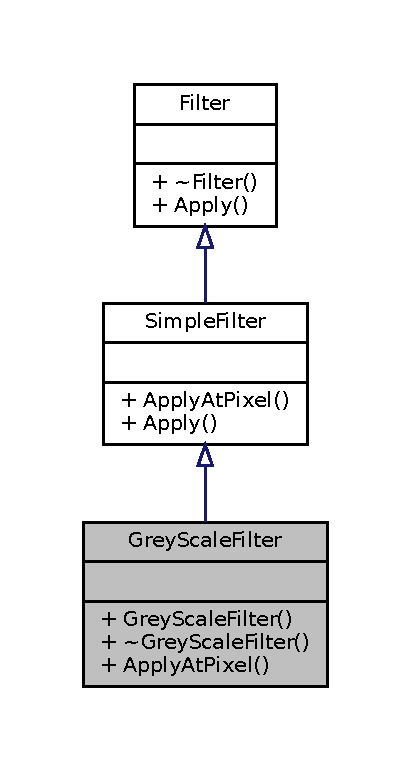
\includegraphics[width=197pt]{classGreyScaleFilter__inherit__graph}
\end{center}
\end{figure}


Collaboration diagram for Grey\+Scale\+Filter\+:\nopagebreak
\begin{figure}[H]
\begin{center}
\leavevmode
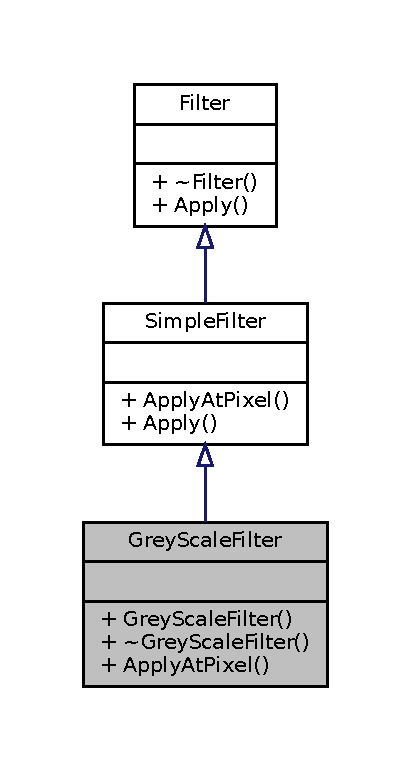
\includegraphics[width=197pt]{classGreyScaleFilter__coll__graph}
\end{center}
\end{figure}
\subsection*{Public Member Functions}
\begin{DoxyCompactItemize}
\item 
\mbox{\Hypertarget{classGreyScaleFilter_a39c97682b954a5c00135eb4c13bddd47}\label{classGreyScaleFilter_a39c97682b954a5c00135eb4c13bddd47}} 
\hyperlink{classGreyScaleFilter_a39c97682b954a5c00135eb4c13bddd47}{Grey\+Scale\+Filter} ()
\begin{DoxyCompactList}\small\item\em Constructor. \end{DoxyCompactList}\item 
\mbox{\Hypertarget{classGreyScaleFilter_a4df05a609fabbc1d4f4c455c53840c68}\label{classGreyScaleFilter_a4df05a609fabbc1d4f4c455c53840c68}} 
\hyperlink{classGreyScaleFilter_a4df05a609fabbc1d4f4c455c53840c68}{$\sim$\+Grey\+Scale\+Filter} ()
\begin{DoxyCompactList}\small\item\em Destructor. \end{DoxyCompactList}\item 
\mbox{\Hypertarget{classGreyScaleFilter_ac781a1ddd205f2d67d1c08481d5ab2e4}\label{classGreyScaleFilter_ac781a1ddd205f2d67d1c08481d5ab2e4}} 
void \hyperlink{classGreyScaleFilter_ac781a1ddd205f2d67d1c08481d5ab2e4}{Apply\+At\+Pixel} (\hyperlink{classColor}{Color} \&p)
\begin{DoxyCompactList}\small\item\em Apply\+At\+Pixel function to be overridden by \hyperlink{classSimpleFilter}{Simple\+Filter} Apply function. \end{DoxyCompactList}\end{DoxyCompactItemize}


\subsection{Detailed Description}
The main class for \hyperlink{classGreyScaleFilter}{Grey\+Scale\+Filter}, extends \hyperlink{classSimpleFilter}{Simple\+Filter}. Overrides the virtual \hyperlink{classGreyScaleFilter_ac781a1ddd205f2d67d1c08481d5ab2e4}{Apply\+At\+Pixel()} function defined in \hyperlink{classSimpleFilter}{Simple\+Filter}. Just calculates the luminance value of each pixel and sets the pixels rgb values to the luminance. 

The documentation for this class was generated from the following files\+:\begin{DoxyCompactItemize}
\item 
/home/user/repo/project/image/include/\hyperlink{greyscale__filter_8h}{greyscale\+\_\+filter.\+h}\item 
/home/user/repo/project/image/src/greyscale\+\_\+filter.\+cc\end{DoxyCompactItemize}

\hypertarget{classHospital}{}\section{Hospital Class Reference}
\label{classHospital}\index{Hospital@{Hospital}}


once our robot is found, we\textquotesingle{}re gonna want to rescue it by taking it to the hospital. Thus we need a hospital entity  




{\ttfamily \#include $<$hospital.\+h$>$}



Inheritance diagram for Hospital\+:\nopagebreak
\begin{figure}[H]
\begin{center}
\leavevmode
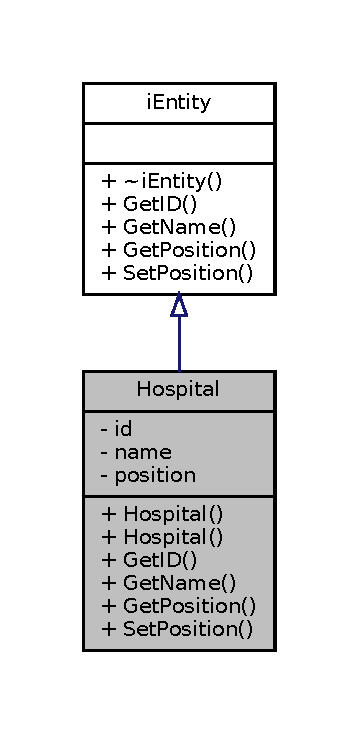
\includegraphics[width=172pt]{classHospital__inherit__graph}
\end{center}
\end{figure}


Collaboration diagram for Hospital\+:\nopagebreak
\begin{figure}[H]
\begin{center}
\leavevmode
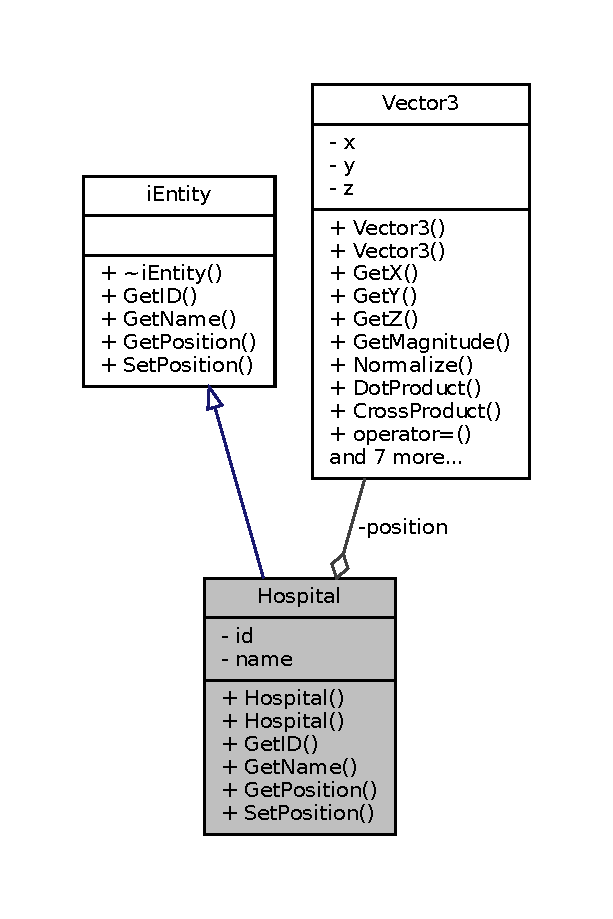
\includegraphics[width=294pt]{classHospital__coll__graph}
\end{center}
\end{figure}
\subsection*{Public Member Functions}
\begin{DoxyCompactItemize}
\item 
\mbox{\Hypertarget{classHospital_a130b3a6c6e3dd35443437e1f5144b1ac}\label{classHospital_a130b3a6c6e3dd35443437e1f5144b1ac}} 
\hyperlink{classHospital_a130b3a6c6e3dd35443437e1f5144b1ac}{Hospital} ()
\begin{DoxyCompactList}\small\item\em default constructor \end{DoxyCompactList}\item 
\mbox{\Hypertarget{classHospital_a04ebe37898559edc3c5bcabe7679366e}\label{classHospital_a04ebe37898559edc3c5bcabe7679366e}} 
\hyperlink{classHospital_a04ebe37898559edc3c5bcabe7679366e}{Hospital} (int \hyperlink{classHospital_ad04682106dbb95ac699a4fc90436db0e}{id}, std\+::string \hyperlink{classHospital_a26fa9b5e5ae30cc8db885c84e02fc2de}{name}, \hyperlink{classVector3}{Vector3} $\ast$pos)
\begin{DoxyCompactList}\small\item\em constructor that takes position argument \end{DoxyCompactList}\item 
\mbox{\Hypertarget{classHospital_a4bb23b897139dd9881654e3a95ae530a}\label{classHospital_a4bb23b897139dd9881654e3a95ae530a}} 
int \hyperlink{classHospital_a4bb23b897139dd9881654e3a95ae530a}{Get\+ID} ()
\begin{DoxyCompactList}\small\item\em Getter\+: returns hospital identification number. \end{DoxyCompactList}\item 
\mbox{\Hypertarget{classHospital_adcbc021db62d8ffb8566f73e79da46a7}\label{classHospital_adcbc021db62d8ffb8566f73e79da46a7}} 
const std\+::string \& \hyperlink{classHospital_adcbc021db62d8ffb8566f73e79da46a7}{Get\+Name} () const
\begin{DoxyCompactList}\small\item\em Getter\+: returns hospital name. \end{DoxyCompactList}\item 
\mbox{\Hypertarget{classHospital_a9da27fc31c98792e720fe34044cac3f0}\label{classHospital_a9da27fc31c98792e720fe34044cac3f0}} 
\hyperlink{classVector3}{Vector3} $\ast$ \hyperlink{classHospital_a9da27fc31c98792e720fe34044cac3f0}{Get\+Position} ()
\begin{DoxyCompactList}\small\item\em Getter\+: returns hospital position. \end{DoxyCompactList}\item 
\mbox{\Hypertarget{classHospital_a712a53eb9795a0362c6aa543a49667eb}\label{classHospital_a712a53eb9795a0362c6aa543a49667eb}} 
void \hyperlink{classHospital_a712a53eb9795a0362c6aa543a49667eb}{Set\+Position} (\hyperlink{classVector3}{Vector3} \&pos)
\begin{DoxyCompactList}\small\item\em Setter\+: updates or initializes position. \end{DoxyCompactList}\end{DoxyCompactItemize}
\subsection*{Private Attributes}
\begin{DoxyCompactItemize}
\item 
\mbox{\Hypertarget{classHospital_ad04682106dbb95ac699a4fc90436db0e}\label{classHospital_ad04682106dbb95ac699a4fc90436db0e}} 
int \hyperlink{classHospital_ad04682106dbb95ac699a4fc90436db0e}{id}
\begin{DoxyCompactList}\small\item\em integer ID of our hospital \end{DoxyCompactList}\item 
\mbox{\Hypertarget{classHospital_a26fa9b5e5ae30cc8db885c84e02fc2de}\label{classHospital_a26fa9b5e5ae30cc8db885c84e02fc2de}} 
std\+::string \hyperlink{classHospital_a26fa9b5e5ae30cc8db885c84e02fc2de}{name}
\begin{DoxyCompactList}\small\item\em hospital name \end{DoxyCompactList}\item 
\mbox{\Hypertarget{classHospital_ae7d66c3913d623f18bb0dde46a624e61}\label{classHospital_ae7d66c3913d623f18bb0dde46a624e61}} 
\hyperlink{classVector3}{Vector3} $\ast$ \hyperlink{classHospital_ae7d66c3913d623f18bb0dde46a624e61}{position}
\begin{DoxyCompactList}\small\item\em 3D vector representing position of hospital \end{DoxyCompactList}\end{DoxyCompactItemize}


\subsection{Detailed Description}
once our robot is found, we\textquotesingle{}re gonna want to rescue it by taking it to the hospital. Thus we need a hospital entity 

The documentation for this class was generated from the following file\+:\begin{DoxyCompactItemize}
\item 
/home/user/repo/project/simulation/include/\hyperlink{hospital_8h}{hospital.\+h}\end{DoxyCompactItemize}

\hypertarget{classHospitalFactory}{}\section{Hospital\+Factory Class Reference}
\label{classHospitalFactory}\index{Hospital\+Factory@{Hospital\+Factory}}


\hyperlink{classHospital}{Hospital} Factory. When called, it creates a new object of type \hyperlink{classHospital}{Hospital}. This factory is never called directly, and is really only used through the composite entity factory.  




{\ttfamily \#include $<$hospital\+\_\+factory.\+h$>$}



Inheritance diagram for Hospital\+Factory\+:\nopagebreak
\begin{figure}[H]
\begin{center}
\leavevmode
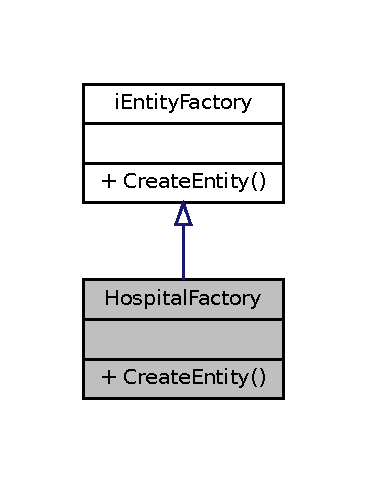
\includegraphics[width=176pt]{classHospitalFactory__inherit__graph}
\end{center}
\end{figure}


Collaboration diagram for Hospital\+Factory\+:\nopagebreak
\begin{figure}[H]
\begin{center}
\leavevmode
\includegraphics[width=176pt]{classHospitalFactory__coll__graph}
\end{center}
\end{figure}
\subsection*{Public Member Functions}
\begin{DoxyCompactItemize}
\item 
\mbox{\Hypertarget{classHospitalFactory_abadf830ce14fcba272af78611c97791d}\label{classHospitalFactory_abadf830ce14fcba272af78611c97791d}} 
\hyperlink{classiEntity}{i\+Entity} $\ast$ \hyperlink{classHospitalFactory_abadf830ce14fcba272af78611c97791d}{Create\+Entity} (picojson\+::object \&entity, \hyperlink{classCamera}{Camera} $\ast$camera)
\begin{DoxyCompactList}\small\item\em checks if type specified is hospital. If so it creates and returns a pointer to our new hospital object. But if the type doesn\textquotesingle{}t match, then it just returns a null pointer. \end{DoxyCompactList}\end{DoxyCompactItemize}


\subsection{Detailed Description}
\hyperlink{classHospital}{Hospital} Factory. When called, it creates a new object of type \hyperlink{classHospital}{Hospital}. This factory is never called directly, and is really only used through the composite entity factory. 

The documentation for this class was generated from the following files\+:\begin{DoxyCompactItemize}
\item 
/home/user/repo/project/simulation/include/\hyperlink{hospital__factory_8h}{hospital\+\_\+factory.\+h}\item 
/home/user/repo/project/simulation/src/hospital\+\_\+factory.\+cc\end{DoxyCompactItemize}

\hypertarget{classHysteresisFilter}{}\section{Hysteresis\+Filter Class Reference}
\label{classHysteresisFilter}\index{Hysteresis\+Filter@{Hysteresis\+Filter}}


The main class for \hyperlink{classHysteresisFilter}{Hysteresis\+Filter}, extends \hyperlink{classFilter}{Filter}. The hysteresis filter takes the output from the double-\/threshold filter and iterates through, changing all \textquotesingle{}weak\textquotesingle{} pixels into \textquotesingle{}strong\textquotesingle{} pixels if any of the surrounding pixels are \textquotesingle{}strong.\textquotesingle{} If not the pixel is set to black.  




{\ttfamily \#include $<$hysteresis\+\_\+filter.\+h$>$}



Inheritance diagram for Hysteresis\+Filter\+:\nopagebreak
\begin{figure}[H]
\begin{center}
\leavevmode
\includegraphics[width=172pt]{classHysteresisFilter__inherit__graph}
\end{center}
\end{figure}


Collaboration diagram for Hysteresis\+Filter\+:\nopagebreak
\begin{figure}[H]
\begin{center}
\leavevmode
\includegraphics[width=172pt]{classHysteresisFilter__coll__graph}
\end{center}
\end{figure}
\subsection*{Public Member Functions}
\begin{DoxyCompactItemize}
\item 
\mbox{\Hypertarget{classHysteresisFilter_af2d6c50bc0cfd609fbf7e90f01b03b1f}\label{classHysteresisFilter_af2d6c50bc0cfd609fbf7e90f01b03b1f}} 
void \hyperlink{classHysteresisFilter_af2d6c50bc0cfd609fbf7e90f01b03b1f}{Apply} (std\+::vector$<$ \hyperlink{classImage}{Image} $\ast$$>$ original, std\+::vector$<$ \hyperlink{classImage}{Image} $\ast$$>$ filtered)
\begin{DoxyCompactList}\small\item\em Apply function to be overridden by \hyperlink{classFilter}{Filter} Apply function. \end{DoxyCompactList}\end{DoxyCompactItemize}


\subsection{Detailed Description}
The main class for \hyperlink{classHysteresisFilter}{Hysteresis\+Filter}, extends \hyperlink{classFilter}{Filter}. The hysteresis filter takes the output from the double-\/threshold filter and iterates through, changing all \textquotesingle{}weak\textquotesingle{} pixels into \textquotesingle{}strong\textquotesingle{} pixels if any of the surrounding pixels are \textquotesingle{}strong.\textquotesingle{} If not the pixel is set to black. 

The documentation for this class was generated from the following files\+:\begin{DoxyCompactItemize}
\item 
/home/user/repo/project/image/include/hysteresis\+\_\+filter.\+h\item 
/home/user/repo/project/image/src/hysteresis\+\_\+filter.\+cc\end{DoxyCompactItemize}

\hypertarget{classICameraController}{}\section{I\+Camera\+Controller Class Reference}
\label{classICameraController}\index{I\+Camera\+Controller@{I\+Camera\+Controller}}


The \hyperlink{classCamera}{Camera} Controller class controls and allows for monitoring of all cameras.  




{\ttfamily \#include $<$camera\+\_\+controller.\+h$>$}



Inheritance diagram for I\+Camera\+Controller\+:\nopagebreak
\begin{figure}[H]
\begin{center}
\leavevmode
\includegraphics[width=215pt]{classICameraController__inherit__graph}
\end{center}
\end{figure}


Collaboration diagram for I\+Camera\+Controller\+:\nopagebreak
\begin{figure}[H]
\begin{center}
\leavevmode
\includegraphics[width=213pt]{classICameraController__coll__graph}
\end{center}
\end{figure}
\subsection*{Public Member Functions}
\begin{DoxyCompactItemize}
\item 
\mbox{\Hypertarget{classICameraController_a7f1b88c7e023ad218d461684dc0d4fe5}\label{classICameraController_a7f1b88c7e023ad218d461684dc0d4fe5}} 
virtual \hyperlink{classICameraController_a7f1b88c7e023ad218d461684dc0d4fe5}{$\sim$\+I\+Camera\+Controller} ()
\begin{DoxyCompactList}\small\item\em Destructor. \end{DoxyCompactList}\item 
\mbox{\Hypertarget{classICameraController_af9fff22819969ca260f7f098f0cdebf4}\label{classICameraController_af9fff22819969ca260f7f098f0cdebf4}} 
virtual void \hyperlink{classICameraController_af9fff22819969ca260f7f098f0cdebf4}{Take\+Picture} (int camera\+Id)=0
\begin{DoxyCompactList}\small\item\em To take a picture with a specific camera, pass in the camera id. \end{DoxyCompactList}\item 
\mbox{\Hypertarget{classICameraController_ad3cf56dc052984b0e31e602f344c35db}\label{classICameraController_ad3cf56dc052984b0e31e602f344c35db}} 
virtual void \hyperlink{classICameraController_ad3cf56dc052984b0e31e602f344c35db}{Add\+Observer} (\hyperlink{classICameraObserver}{I\+Camera\+Observer} \&observer)=0
\begin{DoxyCompactList}\small\item\em Adds a camera observer to monitor cameras. \end{DoxyCompactList}\item 
\mbox{\Hypertarget{classICameraController_a5013bc29f6a0e7794a97646d868bf809}\label{classICameraController_a5013bc29f6a0e7794a97646d868bf809}} 
virtual void \hyperlink{classICameraController_a5013bc29f6a0e7794a97646d868bf809}{Remove\+Observer} (\hyperlink{classICameraObserver}{I\+Camera\+Observer} \&observer)=0
\begin{DoxyCompactList}\small\item\em Removes a camera observer. \end{DoxyCompactList}\end{DoxyCompactItemize}


\subsection{Detailed Description}
The \hyperlink{classCamera}{Camera} Controller class controls and allows for monitoring of all cameras. 

The documentation for this class was generated from the following file\+:\begin{DoxyCompactItemize}
\item 
/home/user/repo/project/simulation/include/camera\+\_\+controller.\+h\end{DoxyCompactItemize}

\hypertarget{classICameraObserver}{}\section{I\+Camera\+Observer Class Reference}
\label{classICameraObserver}\index{I\+Camera\+Observer@{I\+Camera\+Observer}}


A \hyperlink{classCamera}{Camera} Observer monitors results from all cameras. It will process the pictures returned asynchronously and act on results.  




{\ttfamily \#include $<$camera\+\_\+controller.\+h$>$}



Inheritance diagram for I\+Camera\+Observer\+:\nopagebreak
\begin{figure}[H]
\begin{center}
\leavevmode
\includegraphics[width=246pt]{classICameraObserver__inherit__graph}
\end{center}
\end{figure}


Collaboration diagram for I\+Camera\+Observer\+:\nopagebreak
\begin{figure}[H]
\begin{center}
\leavevmode
\includegraphics[width=246pt]{classICameraObserver__coll__graph}
\end{center}
\end{figure}
\subsection*{Public Member Functions}
\begin{DoxyCompactItemize}
\item 
\mbox{\Hypertarget{classICameraObserver_a19344cb93ca790a0311c9c7bcc6e8eec}\label{classICameraObserver_a19344cb93ca790a0311c9c7bcc6e8eec}} 
virtual \hyperlink{classICameraObserver_a19344cb93ca790a0311c9c7bcc6e8eec}{$\sim$\+I\+Camera\+Observer} ()
\begin{DoxyCompactList}\small\item\em Destructor. \end{DoxyCompactList}\item 
virtual \hyperlink{classICameraResult}{I\+Camera\+Result} $\ast$ \hyperlink{classICameraObserver_aec871459f2c429b4334769021b72ec34}{Process\+Images} (int camera\+Id, double x\+Pos, double y\+Pos, double z\+Pos, const std\+::vector$<$ \hyperlink{structRawCameraImage}{Raw\+Camera\+Image} $>$ \&images, picojson\+::object \&details) const =0
\item 
\mbox{\Hypertarget{classICameraObserver_a7d261bd08d570d05032e61b2d5252c88}\label{classICameraObserver_a7d261bd08d570d05032e61b2d5252c88}} 
virtual void \hyperlink{classICameraObserver_a7d261bd08d570d05032e61b2d5252c88}{Image\+Processing\+Complete} (\hyperlink{classICameraResult}{I\+Camera\+Result} $\ast$result)=0
\begin{DoxyCompactList}\small\item\em After the asynchronous image processing is done, this method is called to synchronize the results with the simulation update loop. \end{DoxyCompactList}\end{DoxyCompactItemize}


\subsection{Detailed Description}
A \hyperlink{classCamera}{Camera} Observer monitors results from all cameras. It will process the pictures returned asynchronously and act on results. 

\subsection{Member Function Documentation}
\mbox{\Hypertarget{classICameraObserver_aec871459f2c429b4334769021b72ec34}\label{classICameraObserver_aec871459f2c429b4334769021b72ec34}} 
\index{I\+Camera\+Observer@{I\+Camera\+Observer}!Process\+Images@{Process\+Images}}
\index{Process\+Images@{Process\+Images}!I\+Camera\+Observer@{I\+Camera\+Observer}}
\subsubsection{\texorpdfstring{Process\+Images()}{ProcessImages()}}
{\footnotesize\ttfamily virtual \hyperlink{classICameraResult}{I\+Camera\+Result}$\ast$ I\+Camera\+Observer\+::\+Process\+Images (\begin{DoxyParamCaption}\item[{int}]{camera\+Id,  }\item[{double}]{x\+Pos,  }\item[{double}]{y\+Pos,  }\item[{double}]{z\+Pos,  }\item[{const std\+::vector$<$ \hyperlink{structRawCameraImage}{Raw\+Camera\+Image} $>$ \&}]{images,  }\item[{picojson\+::object \&}]{details }\end{DoxyParamCaption}) const\hspace{0.3cm}{\ttfamily [pure virtual]}}

Processes images asynchronously after a picture has been taken. This method will pass in the camera position and the raw images stored in jpg format. Do all your image processing here so that it does not slow down your simulation. The result will be passed to the Image\+Processing\+Complete(...) method. 

Implemented in \hyperlink{classCamera_a792611ad34a1c595b61b7c72ce1d5e32}{Camera}.



The documentation for this class was generated from the following file\+:\begin{DoxyCompactItemize}
\item 
/home/user/repo/project/simulation/include/camera\+\_\+controller.\+h\end{DoxyCompactItemize}

\hypertarget{classICameraResult}{}\section{I\+Camera\+Result Class Reference}
\label{classICameraResult}\index{I\+Camera\+Result@{I\+Camera\+Result}}


The result returned from the image processing.  




{\ttfamily \#include $<$camera\+\_\+controller.\+h$>$}



Inheritance diagram for I\+Camera\+Result\+:\nopagebreak
\begin{figure}[H]
\begin{center}
\leavevmode
\includegraphics[width=209pt]{classICameraResult__inherit__graph}
\end{center}
\end{figure}


Collaboration diagram for I\+Camera\+Result\+:\nopagebreak
\begin{figure}[H]
\begin{center}
\leavevmode
\includegraphics[width=195pt]{classICameraResult__coll__graph}
\end{center}
\end{figure}
\subsection*{Public Member Functions}
\begin{DoxyCompactItemize}
\item 
\mbox{\Hypertarget{classICameraResult_a6c8f4f6c3748c00236bd588cf9410f8b}\label{classICameraResult_a6c8f4f6c3748c00236bd588cf9410f8b}} 
virtual \hyperlink{classICameraResult_a6c8f4f6c3748c00236bd588cf9410f8b}{$\sim$\+I\+Camera\+Result} ()
\begin{DoxyCompactList}\small\item\em destructor \end{DoxyCompactList}\end{DoxyCompactItemize}


\subsection{Detailed Description}
The result returned from the image processing. 

The documentation for this class was generated from the following file\+:\begin{DoxyCompactItemize}
\item 
/home/user/repo/project/simulation/include/camera\+\_\+controller.\+h\end{DoxyCompactItemize}

\hypertarget{classiEntity}{}\section{i\+Entity Class Reference}
\label{classiEntity}\index{i\+Entity@{i\+Entity}}


The base class for all entities. Drones, Robots, Hospitals, and Recharge Stations are all entities. This class is abstract, so it\textquotesingle{}s not meant to be instantiated.  




{\ttfamily \#include $<$i\+\_\+entity.\+h$>$}



Inheritance diagram for i\+Entity\+:\nopagebreak
\begin{figure}[H]
\begin{center}
\leavevmode
\includegraphics[width=350pt]{classiEntity__inherit__graph}
\end{center}
\end{figure}


Collaboration diagram for i\+Entity\+:\nopagebreak
\begin{figure}[H]
\begin{center}
\leavevmode
\includegraphics[width=172pt]{classiEntity__coll__graph}
\end{center}
\end{figure}
\subsection*{Public Member Functions}
\begin{DoxyCompactItemize}
\item 
\mbox{\Hypertarget{classiEntity_ab8633da01cab1d5a6aa565ac45a74c59}\label{classiEntity_ab8633da01cab1d5a6aa565ac45a74c59}} 
virtual \hyperlink{classiEntity_ab8633da01cab1d5a6aa565ac45a74c59}{$\sim$i\+Entity} ()
\begin{DoxyCompactList}\small\item\em Destructor. \end{DoxyCompactList}\item 
\mbox{\Hypertarget{classiEntity_afff83e95a9777dfaa7cf48bad6fbb79c}\label{classiEntity_afff83e95a9777dfaa7cf48bad6fbb79c}} 
virtual int \hyperlink{classiEntity_afff83e95a9777dfaa7cf48bad6fbb79c}{Get\+ID} ()=0
\begin{DoxyCompactList}\small\item\em Getter\+: returns entity identification number. \end{DoxyCompactList}\item 
\mbox{\Hypertarget{classiEntity_a4c71545cc2dec140595b5c1e1be8ac32}\label{classiEntity_a4c71545cc2dec140595b5c1e1be8ac32}} 
virtual const std\+::string \& \hyperlink{classiEntity_a4c71545cc2dec140595b5c1e1be8ac32}{Get\+Name} () const =0
\begin{DoxyCompactList}\small\item\em Getter\+: returns entity name. \end{DoxyCompactList}\item 
\mbox{\Hypertarget{classiEntity_a2e94d2de4d37792e6f491405ac259aeb}\label{classiEntity_a2e94d2de4d37792e6f491405ac259aeb}} 
virtual \hyperlink{classVector3}{Vector3} $\ast$ \hyperlink{classiEntity_a2e94d2de4d37792e6f491405ac259aeb}{Get\+Position} ()=0
\begin{DoxyCompactList}\small\item\em Getter\+: returns entity position. \end{DoxyCompactList}\item 
\mbox{\Hypertarget{classiEntity_afa1966ac1964902c1e69907307ca03d4}\label{classiEntity_afa1966ac1964902c1e69907307ca03d4}} 
virtual void \hyperlink{classiEntity_afa1966ac1964902c1e69907307ca03d4}{Set\+Position} (\hyperlink{classVector3}{Vector3} \&pos)=0
\begin{DoxyCompactList}\small\item\em Setter\+: updates or initializes position. \end{DoxyCompactList}\end{DoxyCompactItemize}


\subsection{Detailed Description}
The base class for all entities. Drones, Robots, Hospitals, and Recharge Stations are all entities. This class is abstract, so it\textquotesingle{}s not meant to be instantiated. 

The documentation for this class was generated from the following file\+:\begin{DoxyCompactItemize}
\item 
/home/user/repo/project/simulation/include/i\+\_\+entity.\+h\end{DoxyCompactItemize}

\hypertarget{classiEntityFactory}{}\section{i\+Entity\+Factory Class Reference}
\label{classiEntityFactory}\index{i\+Entity\+Factory@{i\+Entity\+Factory}}


Entity factory interface. Used for our abstract factory method for making new entity objects at run time. Implementation is carried out by \hyperlink{classDroneFactory}{Drone\+Factory}, \hyperlink{classRobotFactory}{Robot\+Factory}, hospital\+Factory, and \hyperlink{classRechargeStationFactory}{Recharge\+Station\+Factory}.  




{\ttfamily \#include $<$i\+\_\+entity\+\_\+factory.\+h$>$}



Inheritance diagram for i\+Entity\+Factory\+:\nopagebreak
\begin{figure}[H]
\begin{center}
\leavevmode
\includegraphics[width=350pt]{classiEntityFactory__inherit__graph}
\end{center}
\end{figure}


Collaboration diagram for i\+Entity\+Factory\+:\nopagebreak
\begin{figure}[H]
\begin{center}
\leavevmode
\includegraphics[width=176pt]{classiEntityFactory__coll__graph}
\end{center}
\end{figure}
\subsection*{Public Member Functions}
\begin{DoxyCompactItemize}
\item 
\mbox{\Hypertarget{classiEntityFactory_ab1ce8456ec513534a056c446d417aab7}\label{classiEntityFactory_ab1ce8456ec513534a056c446d417aab7}} 
virtual \hyperlink{classiEntity}{i\+Entity} $\ast$ {\bfseries Create\+Entity} (picojson\+::object \&entity, \hyperlink{classCamera}{Camera} $\ast$camera)=0
\end{DoxyCompactItemize}


\subsection{Detailed Description}
Entity factory interface. Used for our abstract factory method for making new entity objects at run time. Implementation is carried out by \hyperlink{classDroneFactory}{Drone\+Factory}, \hyperlink{classRobotFactory}{Robot\+Factory}, hospital\+Factory, and \hyperlink{classRechargeStationFactory}{Recharge\+Station\+Factory}. 

The documentation for this class was generated from the following file\+:\begin{DoxyCompactItemize}
\item 
/home/user/repo/project/simulation/include/\hyperlink{i__entity__factory_8h}{i\+\_\+entity\+\_\+factory.\+h}\end{DoxyCompactItemize}

\hypertarget{classiLogger}{}\section{i\+Logger Class Reference}
\label{classiLogger}\index{i\+Logger@{i\+Logger}}


data logger interface. Used to log data on our drone for reasons unbenounced to me. If we wanted to further optimize our drone search and rescue system, we could use a machine learning algorithm to go through our data output files to find the optimal search pattern. This is a composite pattern and has two main logger methods. One for outputing to the terminal screen, and one for saving in a C\+SV file.  




{\ttfamily \#include $<$i\+\_\+logger.\+h$>$}



Inheritance diagram for i\+Logger\+:\nopagebreak
\begin{figure}[H]
\begin{center}
\leavevmode
\includegraphics[width=350pt]{classiLogger__inherit__graph}
\end{center}
\end{figure}


Collaboration diagram for i\+Logger\+:\nopagebreak
\begin{figure}[H]
\begin{center}
\leavevmode
\includegraphics[width=133pt]{classiLogger__coll__graph}
\end{center}
\end{figure}
\subsection*{Public Member Functions}
\begin{DoxyCompactItemize}
\item 
\mbox{\Hypertarget{classiLogger_a1809fbe5bc65d1c18de646e5173aa304}\label{classiLogger_a1809fbe5bc65d1c18de646e5173aa304}} 
virtual void \hyperlink{classiLogger_a1809fbe5bc65d1c18de646e5173aa304}{Log} (\hyperlink{classVector3}{Vector3} $\ast$p, \hyperlink{classVector3}{Vector3} $\ast$d, double t)=0
\begin{DoxyCompactList}\small\item\em log position, direction, and elapsed time of drone. Called every time we update. \end{DoxyCompactList}\end{DoxyCompactItemize}


\subsection{Detailed Description}
data logger interface. Used to log data on our drone for reasons unbenounced to me. If we wanted to further optimize our drone search and rescue system, we could use a machine learning algorithm to go through our data output files to find the optimal search pattern. This is a composite pattern and has two main logger methods. One for outputing to the terminal screen, and one for saving in a C\+SV file. 

The documentation for this class was generated from the following file\+:\begin{DoxyCompactItemize}
\item 
/home/user/repo/project/simulation/include/\hyperlink{i__logger_8h}{i\+\_\+logger.\+h}\end{DoxyCompactItemize}

\hypertarget{classImage}{}\section{Image Class Reference}
\label{classImage}\index{Image@{Image}}


The main class for \hyperlink{classImage}{Image}. \hyperlink{classImage}{Image} is represented as a big unsigned character array, and alters values inside the image by using the color class. Class just contains getters, setters, and the big 3.  




{\ttfamily \#include $<$image.\+h$>$}



Collaboration diagram for Image\+:\nopagebreak
\begin{figure}[H]
\begin{center}
\leavevmode
\includegraphics[width=212pt]{classImage__coll__graph}
\end{center}
\end{figure}
\subsection*{Public Member Functions}
\begin{DoxyCompactItemize}
\item 
\mbox{\Hypertarget{classImage_a58edd1c45b4faeb5f789b0d036d02313}\label{classImage_a58edd1c45b4faeb5f789b0d036d02313}} 
\hyperlink{classImage_a58edd1c45b4faeb5f789b0d036d02313}{Image} ()
\begin{DoxyCompactList}\small\item\em Constructor for no arguments. \end{DoxyCompactList}\item 
\mbox{\Hypertarget{classImage_afb0339b802ed560e69eb07358d30198f}\label{classImage_afb0339b802ed560e69eb07358d30198f}} 
\hyperlink{classImage_afb0339b802ed560e69eb07358d30198f}{Image} (int width, int height)
\begin{DoxyCompactList}\small\item\em Constructor for int width and int height arguments. \end{DoxyCompactList}\item 
\mbox{\Hypertarget{classImage_abb20937b3256735f0f7549d1b5e9c10d}\label{classImage_abb20937b3256735f0f7549d1b5e9c10d}} 
\hyperlink{classImage_abb20937b3256735f0f7549d1b5e9c10d}{Image} (std\+::string filename)
\begin{DoxyCompactList}\small\item\em Constructor for string filename argument. \end{DoxyCompactList}\item 
\hyperlink{classImage_a50994051928f5e597226aea5139aea6d}{Image} (unsigned char $\ast$buffer, int width, int height)
\begin{DoxyCompactList}\small\item\em Construct a new \hyperlink{classImage}{Image} object with a buffer as the argument. \end{DoxyCompactList}\item 
\mbox{\Hypertarget{classImage_aa44ed77d00d96d2c878b050835f828c4}\label{classImage_aa44ed77d00d96d2c878b050835f828c4}} 
\hyperlink{classImage_aa44ed77d00d96d2c878b050835f828c4}{Image} (const \hyperlink{classImage}{Image} \&img)
\begin{DoxyCompactList}\small\item\em Constructor for \hyperlink{classImage}{Image} image argument. \end{DoxyCompactList}\item 
\mbox{\Hypertarget{classImage_a0294f63700543e11c0f0da85601c7ae5}\label{classImage_a0294f63700543e11c0f0da85601c7ae5}} 
\hyperlink{classImage_a0294f63700543e11c0f0da85601c7ae5}{$\sim$\+Image} ()
\begin{DoxyCompactList}\small\item\em Destructor. \end{DoxyCompactList}\item 
\mbox{\Hypertarget{classImage_a3a9b278005e0731a93fe1d5d2cff7104}\label{classImage_a3a9b278005e0731a93fe1d5d2cff7104}} 
void \hyperlink{classImage_a3a9b278005e0731a93fe1d5d2cff7104}{Save\+As} (std\+::string filename)
\begin{DoxyCompactList}\small\item\em Save taking in a string argument filename to save to. \end{DoxyCompactList}\item 
int \hyperlink{classImage_a4ab80d76fd124fd9de9b4fca8ae16186}{Get\+Width} ()
\begin{DoxyCompactList}\small\item\em Width getter. \end{DoxyCompactList}\item 
int \hyperlink{classImage_a4d6de643ee334ff52c85da9a62d9297d}{Get\+Height} ()
\begin{DoxyCompactList}\small\item\em Height getter. \end{DoxyCompactList}\item 
int \hyperlink{classImage_a04e02c5aa54d26422bbaa777b08de4c9}{Get\+Component\+Num} ()
\begin{DoxyCompactList}\small\item\em Component number getter. \end{DoxyCompactList}\item 
int \hyperlink{classImage_ad9ce272b2befc075fa720ac25f673202}{Get\+Size} ()
\begin{DoxyCompactList}\small\item\em Size getter. \end{DoxyCompactList}\item 
\mbox{\Hypertarget{classImage_a5b9ba06409ad38e86a035ad18d8204d2}\label{classImage_a5b9ba06409ad38e86a035ad18d8204d2}} 
void \hyperlink{classImage_a5b9ba06409ad38e86a035ad18d8204d2}{Get\+Pixel} (int x, int y, \hyperlink{classColor}{Color} \&p)
\begin{DoxyCompactList}\small\item\em Pixel getter given arguments int x, int y, \hyperlink{classColor}{Color} p. \end{DoxyCompactList}\item 
\mbox{\Hypertarget{classImage_a88e6e6e7cbe530c84c17a342fa2eaf40}\label{classImage_a88e6e6e7cbe530c84c17a342fa2eaf40}} 
void \hyperlink{classImage_a88e6e6e7cbe530c84c17a342fa2eaf40}{Set\+Pixel} (int x, int y, \hyperlink{classColor}{Color} \&p)
\begin{DoxyCompactList}\small\item\em Pixel setter given arguments int x, int y, \hyperlink{classColor}{Color} p. \end{DoxyCompactList}\item 
void \hyperlink{classImage_a558cfcb26f9f8abc82c32d85a25332f7}{Set\+Pixel\+Data} (int x, int y, \hyperlink{classColor}{Color} \&p)
\begin{DoxyCompactList}\small\item\em Set the Pixel Data object, does not multiply values by 255. \end{DoxyCompactList}\item 
unsigned char $\ast$ \hyperlink{classImage_a6337e9b91fb0aeb0b482d7e933543608}{Get\+Data} ()
\begin{DoxyCompactList}\small\item\em Get the Data object. \end{DoxyCompactList}\item 
void \hyperlink{classImage_a5fab96b8b5e873488b72185639790c92}{Set\+Data} (unsigned char $\ast$data)
\begin{DoxyCompactList}\small\item\em Set the Data object. \end{DoxyCompactList}\item 
\mbox{\Hypertarget{classImage_a4da7f72e4063bd0764caa635c0e0aaae}\label{classImage_a4da7f72e4063bd0764caa635c0e0aaae}} 
void \hyperlink{classImage_a4da7f72e4063bd0764caa635c0e0aaae}{operator=} (const \hyperlink{classImage}{Image} \&img)
\begin{DoxyCompactList}\small\item\em = operator given an \hyperlink{classImage}{Image} image \end{DoxyCompactList}\end{DoxyCompactItemize}
\subsection*{Private Attributes}
\begin{DoxyCompactItemize}
\item 
\mbox{\Hypertarget{classImage_a9a2c38d0f90325c4526e658463638a3d}\label{classImage_a9a2c38d0f90325c4526e658463638a3d}} 
unsigned char $\ast$ {\bfseries image}
\item 
\mbox{\Hypertarget{classImage_ab8d12f635013c04159cd4d3d972bac88}\label{classImage_ab8d12f635013c04159cd4d3d972bac88}} 
int {\bfseries width}
\item 
\mbox{\Hypertarget{classImage_a51df43db420c9c0b57536cb2dd36de5c}\label{classImage_a51df43db420c9c0b57536cb2dd36de5c}} 
int {\bfseries height}
\item 
\mbox{\Hypertarget{classImage_ac6bbfcf18fdb753ab56cd0d6e21b8d76}\label{classImage_ac6bbfcf18fdb753ab56cd0d6e21b8d76}} 
int {\bfseries components}
\item 
\mbox{\Hypertarget{classImage_af9a53c18c62335dae6139bfa04667cc5}\label{classImage_af9a53c18c62335dae6139bfa04667cc5}} 
int {\bfseries size}
\end{DoxyCompactItemize}


\subsection{Detailed Description}
The main class for \hyperlink{classImage}{Image}. \hyperlink{classImage}{Image} is represented as a big unsigned character array, and alters values inside the image by using the color class. Class just contains getters, setters, and the big 3. 

\subsection{Constructor \& Destructor Documentation}
\mbox{\Hypertarget{classImage_a50994051928f5e597226aea5139aea6d}\label{classImage_a50994051928f5e597226aea5139aea6d}} 
\index{Image@{Image}!Image@{Image}}
\index{Image@{Image}!Image@{Image}}
\subsubsection{\texorpdfstring{Image()}{Image()}}
{\footnotesize\ttfamily Image\+::\+Image (\begin{DoxyParamCaption}\item[{unsigned char $\ast$}]{buffer,  }\item[{int}]{width,  }\item[{int}]{height }\end{DoxyParamCaption})}



Construct a new \hyperlink{classImage}{Image} object with a buffer as the argument. 


\begin{DoxyParams}{Parameters}
{\em buffer} & \\
\hline
\end{DoxyParams}


\subsection{Member Function Documentation}
\mbox{\Hypertarget{classImage_a04e02c5aa54d26422bbaa777b08de4c9}\label{classImage_a04e02c5aa54d26422bbaa777b08de4c9}} 
\index{Image@{Image}!Get\+Component\+Num@{Get\+Component\+Num}}
\index{Get\+Component\+Num@{Get\+Component\+Num}!Image@{Image}}
\subsubsection{\texorpdfstring{Get\+Component\+Num()}{GetComponentNum()}}
{\footnotesize\ttfamily int Image\+::\+Get\+Component\+Num (\begin{DoxyParamCaption}{ }\end{DoxyParamCaption})}



Component number getter. 

\begin{DoxyReturn}{Returns}
Int component\+Num. 
\end{DoxyReturn}
\mbox{\Hypertarget{classImage_a6337e9b91fb0aeb0b482d7e933543608}\label{classImage_a6337e9b91fb0aeb0b482d7e933543608}} 
\index{Image@{Image}!Get\+Data@{Get\+Data}}
\index{Get\+Data@{Get\+Data}!Image@{Image}}
\subsubsection{\texorpdfstring{Get\+Data()}{GetData()}}
{\footnotesize\ttfamily unsigned char $\ast$ Image\+::\+Get\+Data (\begin{DoxyParamCaption}{ }\end{DoxyParamCaption})}



Get the Data object. 

\begin{DoxyReturn}{Returns}
unsigned$\ast$ 
\end{DoxyReturn}
\mbox{\Hypertarget{classImage_a4d6de643ee334ff52c85da9a62d9297d}\label{classImage_a4d6de643ee334ff52c85da9a62d9297d}} 
\index{Image@{Image}!Get\+Height@{Get\+Height}}
\index{Get\+Height@{Get\+Height}!Image@{Image}}
\subsubsection{\texorpdfstring{Get\+Height()}{GetHeight()}}
{\footnotesize\ttfamily int Image\+::\+Get\+Height (\begin{DoxyParamCaption}{ }\end{DoxyParamCaption})}



Height getter. 

\begin{DoxyReturn}{Returns}
Int height. 
\end{DoxyReturn}
\mbox{\Hypertarget{classImage_ad9ce272b2befc075fa720ac25f673202}\label{classImage_ad9ce272b2befc075fa720ac25f673202}} 
\index{Image@{Image}!Get\+Size@{Get\+Size}}
\index{Get\+Size@{Get\+Size}!Image@{Image}}
\subsubsection{\texorpdfstring{Get\+Size()}{GetSize()}}
{\footnotesize\ttfamily int Image\+::\+Get\+Size (\begin{DoxyParamCaption}{ }\end{DoxyParamCaption})}



Size getter. 

\begin{DoxyReturn}{Returns}
Int size. 
\end{DoxyReturn}
\mbox{\Hypertarget{classImage_a4ab80d76fd124fd9de9b4fca8ae16186}\label{classImage_a4ab80d76fd124fd9de9b4fca8ae16186}} 
\index{Image@{Image}!Get\+Width@{Get\+Width}}
\index{Get\+Width@{Get\+Width}!Image@{Image}}
\subsubsection{\texorpdfstring{Get\+Width()}{GetWidth()}}
{\footnotesize\ttfamily int Image\+::\+Get\+Width (\begin{DoxyParamCaption}{ }\end{DoxyParamCaption})}



Width getter. 

\begin{DoxyReturn}{Returns}
Int width. 
\end{DoxyReturn}
\mbox{\Hypertarget{classImage_a5fab96b8b5e873488b72185639790c92}\label{classImage_a5fab96b8b5e873488b72185639790c92}} 
\index{Image@{Image}!Set\+Data@{Set\+Data}}
\index{Set\+Data@{Set\+Data}!Image@{Image}}
\subsubsection{\texorpdfstring{Set\+Data()}{SetData()}}
{\footnotesize\ttfamily void Image\+::\+Set\+Data (\begin{DoxyParamCaption}\item[{unsigned char $\ast$}]{data }\end{DoxyParamCaption})}



Set the Data object. 


\begin{DoxyParams}{Parameters}
{\em data} & \\
\hline
\end{DoxyParams}
\mbox{\Hypertarget{classImage_a558cfcb26f9f8abc82c32d85a25332f7}\label{classImage_a558cfcb26f9f8abc82c32d85a25332f7}} 
\index{Image@{Image}!Set\+Pixel\+Data@{Set\+Pixel\+Data}}
\index{Set\+Pixel\+Data@{Set\+Pixel\+Data}!Image@{Image}}
\subsubsection{\texorpdfstring{Set\+Pixel\+Data()}{SetPixelData()}}
{\footnotesize\ttfamily void Image\+::\+Set\+Pixel\+Data (\begin{DoxyParamCaption}\item[{int}]{x,  }\item[{int}]{y,  }\item[{\hyperlink{classColor}{Color} \&}]{p }\end{DoxyParamCaption})}



Set the Pixel Data object, does not multiply values by 255. 


\begin{DoxyParams}{Parameters}
{\em x} & \\
\hline
{\em y} & \\
\hline
{\em p} & \\
\hline
\end{DoxyParams}


The documentation for this class was generated from the following files\+:\begin{DoxyCompactItemize}
\item 
/home/user/repo/project/image/include/\hyperlink{image_8h}{image.\+h}\item 
/home/user/repo/project/image/src/image.\+cc\end{DoxyCompactItemize}

\hypertarget{classImageProcessingFacade}{}\section{Image\+Processing\+Facade Class Reference}
\label{classImageProcessingFacade}\index{Image\+Processing\+Facade@{Image\+Processing\+Facade}}


The image processing facade, enables functionality with the image processor with easy to use functions that enable complicated functions with easy use.  




{\ttfamily \#include $<$image\+\_\+processing\+\_\+facade.\+h$>$}



Collaboration diagram for Image\+Processing\+Facade\+:\nopagebreak
\begin{figure}[H]
\begin{center}
\leavevmode
\includegraphics[width=270pt]{classImageProcessingFacade__coll__graph}
\end{center}
\end{figure}
\subsection*{Public Member Functions}
\begin{DoxyCompactItemize}
\item 
\mbox{\Hypertarget{classImageProcessingFacade_ac8691c5159915b0f48d21a24576666ec}\label{classImageProcessingFacade_ac8691c5159915b0f48d21a24576666ec}} 
\hyperlink{classImageProcessingFacade_ac8691c5159915b0f48d21a24576666ec}{Image\+Processing\+Facade} ()
\begin{DoxyCompactList}\small\item\em Construct a new \hyperlink{classImage}{Image} Processing Facade object. \end{DoxyCompactList}\item 
void \hyperlink{classImageProcessingFacade_a320be6a053c96f9725f6526b0f4734c4}{Run\+Canny\+Edge\+Detect} (\hyperlink{classImage}{Image} $\ast$image, \hyperlink{classImage}{Image} $\ast$canny\+Image)
\begin{DoxyCompactList}\small\item\em Runs the canny edge detect filter from image processor. \end{DoxyCompactList}\item 
void \hyperlink{classImageProcessingFacade_ad65fe6e5f6db9aa5c45235b8e4486659}{Blob\+Detect} (\hyperlink{classImage}{Image} $\ast$image, \hyperlink{classImage}{Image} $\ast$blob\+Detect)
\begin{DoxyCompactList}\small\item\em Runs blob detect filter from image processor. \end{DoxyCompactList}\end{DoxyCompactItemize}
\subsection*{Private Attributes}
\begin{DoxyCompactItemize}
\item 
\mbox{\Hypertarget{classImageProcessingFacade_ada20bac7f9fd22337ff810fd1786b5ee}\label{classImageProcessingFacade_ada20bac7f9fd22337ff810fd1786b5ee}} 
\hyperlink{classFilter}{Filter} $\ast$ \hyperlink{classImageProcessingFacade_ada20bac7f9fd22337ff810fd1786b5ee}{canny\+Edge\+Detect\+Filter}
\begin{DoxyCompactList}\small\item\em Reference to canny edge detect filter. \end{DoxyCompactList}\item 
\mbox{\Hypertarget{classImageProcessingFacade_a19ac9e618b71451afe7322eb0886aad8}\label{classImageProcessingFacade_a19ac9e618b71451afe7322eb0886aad8}} 
\hyperlink{classFilter}{Filter} $\ast$ \hyperlink{classImageProcessingFacade_a19ac9e618b71451afe7322eb0886aad8}{blob\+Detect\+Filter}
\begin{DoxyCompactList}\small\item\em Reference to blob detect filter. \end{DoxyCompactList}\end{DoxyCompactItemize}


\subsection{Detailed Description}
The image processing facade, enables functionality with the image processor with easy to use functions that enable complicated functions with easy use. 

\subsection{Member Function Documentation}
\mbox{\Hypertarget{classImageProcessingFacade_ad65fe6e5f6db9aa5c45235b8e4486659}\label{classImageProcessingFacade_ad65fe6e5f6db9aa5c45235b8e4486659}} 
\index{Image\+Processing\+Facade@{Image\+Processing\+Facade}!Blob\+Detect@{Blob\+Detect}}
\index{Blob\+Detect@{Blob\+Detect}!Image\+Processing\+Facade@{Image\+Processing\+Facade}}
\subsubsection{\texorpdfstring{Blob\+Detect()}{BlobDetect()}}
{\footnotesize\ttfamily void Image\+Processing\+Facade\+::\+Blob\+Detect (\begin{DoxyParamCaption}\item[{\hyperlink{classImage}{Image} $\ast$}]{image,  }\item[{\hyperlink{classImage}{Image} $\ast$}]{blob\+Detect }\end{DoxyParamCaption})\hspace{0.3cm}{\ttfamily [inline]}}



Runs blob detect filter from image processor. 


\begin{DoxyParams}{Parameters}
{\em image} & \\
\hline
{\em blob\+Detect} & \\
\hline
\end{DoxyParams}
\mbox{\Hypertarget{classImageProcessingFacade_a320be6a053c96f9725f6526b0f4734c4}\label{classImageProcessingFacade_a320be6a053c96f9725f6526b0f4734c4}} 
\index{Image\+Processing\+Facade@{Image\+Processing\+Facade}!Run\+Canny\+Edge\+Detect@{Run\+Canny\+Edge\+Detect}}
\index{Run\+Canny\+Edge\+Detect@{Run\+Canny\+Edge\+Detect}!Image\+Processing\+Facade@{Image\+Processing\+Facade}}
\subsubsection{\texorpdfstring{Run\+Canny\+Edge\+Detect()}{RunCannyEdgeDetect()}}
{\footnotesize\ttfamily void Image\+Processing\+Facade\+::\+Run\+Canny\+Edge\+Detect (\begin{DoxyParamCaption}\item[{\hyperlink{classImage}{Image} $\ast$}]{image,  }\item[{\hyperlink{classImage}{Image} $\ast$}]{canny\+Image }\end{DoxyParamCaption})\hspace{0.3cm}{\ttfamily [inline]}}



Runs the canny edge detect filter from image processor. 


\begin{DoxyParams}{Parameters}
{\em image} & \\
\hline
\end{DoxyParams}
\begin{DoxyReturn}{Returns}
Image$\ast$ 
\end{DoxyReturn}


The documentation for this class was generated from the following file\+:\begin{DoxyCompactItemize}
\item 
/home/user/repo/project/simulation/include/\hyperlink{image__processing__facade_8h}{image\+\_\+processing\+\_\+facade.\+h}\end{DoxyCompactItemize}

\hypertarget{classiMovableEntity}{}\section{i\+Movable\+Entity Class Reference}
\label{classiMovableEntity}\index{i\+Movable\+Entity@{i\+Movable\+Entity}}


derived class of entity. This is an abstract class that represents entities that move. This class gets implemented by the \hyperlink{classDrone}{Drone} and \hyperlink{classRobot}{Robot} entities.  




{\ttfamily \#include $<$i\+\_\+movable\+\_\+entity.\+h$>$}



Inheritance diagram for i\+Movable\+Entity\+:\nopagebreak
\begin{figure}[H]
\begin{center}
\leavevmode
\includegraphics[height=550pt]{classiMovableEntity__inherit__graph}
\end{center}
\end{figure}


Collaboration diagram for i\+Movable\+Entity\+:\nopagebreak
\begin{figure}[H]
\begin{center}
\leavevmode
\includegraphics[width=196pt]{classiMovableEntity__coll__graph}
\end{center}
\end{figure}
\subsection*{Public Member Functions}
\begin{DoxyCompactItemize}
\item 
\mbox{\Hypertarget{classiMovableEntity_a7ef5def1645b30429c910bfd6a6b67ef}\label{classiMovableEntity_a7ef5def1645b30429c910bfd6a6b67ef}} 
virtual \hyperlink{classiMovableEntity_a7ef5def1645b30429c910bfd6a6b67ef}{$\sim$i\+Movable\+Entity} ()
\begin{DoxyCompactList}\small\item\em Destructor. \end{DoxyCompactList}\item 
\mbox{\Hypertarget{classiMovableEntity_a1723b1c151cd37c60d4dc8925e8fa571}\label{classiMovableEntity_a1723b1c151cd37c60d4dc8925e8fa571}} 
virtual int \hyperlink{classiMovableEntity_a1723b1c151cd37c60d4dc8925e8fa571}{Get\+ID} ()=0
\begin{DoxyCompactList}\small\item\em getter\+: returns entity identification number \end{DoxyCompactList}\item 
\mbox{\Hypertarget{classiMovableEntity_a580ed40373852e32dd81bc3a92903d3e}\label{classiMovableEntity_a580ed40373852e32dd81bc3a92903d3e}} 
virtual const std\+::string \& \hyperlink{classiMovableEntity_a580ed40373852e32dd81bc3a92903d3e}{Get\+Name} () const =0
\begin{DoxyCompactList}\small\item\em getter\+: returns entity name \end{DoxyCompactList}\item 
\mbox{\Hypertarget{classiMovableEntity_aba07ec07fb682e277e3e997256bda000}\label{classiMovableEntity_aba07ec07fb682e277e3e997256bda000}} 
virtual \hyperlink{classVector3}{Vector3} $\ast$ \hyperlink{classiMovableEntity_aba07ec07fb682e277e3e997256bda000}{Get\+Position} ()=0
\begin{DoxyCompactList}\small\item\em getter\+: returns entity position \end{DoxyCompactList}\item 
\mbox{\Hypertarget{classiMovableEntity_afbf41c5d1499bfe87054a53de7d87fe8}\label{classiMovableEntity_afbf41c5d1499bfe87054a53de7d87fe8}} 
virtual void \hyperlink{classiMovableEntity_afbf41c5d1499bfe87054a53de7d87fe8}{Set\+Position} (\hyperlink{classVector3}{Vector3} \&pos)=0
\begin{DoxyCompactList}\small\item\em setter\+: updates or initializes position \end{DoxyCompactList}\item 
\mbox{\Hypertarget{classiMovableEntity_a1285f3317ed9b2d59d8701711b5c3e67}\label{classiMovableEntity_a1285f3317ed9b2d59d8701711b5c3e67}} 
virtual \hyperlink{classVector3}{Vector3} $\ast$ \hyperlink{classiMovableEntity_a1285f3317ed9b2d59d8701711b5c3e67}{Get\+Velocity} ()=0
\begin{DoxyCompactList}\small\item\em getter\+: returns entity\textquotesingle{}s velocity \end{DoxyCompactList}\item 
\mbox{\Hypertarget{classiMovableEntity_ab1b67096acd0e25f97ecceeeeed1c972}\label{classiMovableEntity_ab1b67096acd0e25f97ecceeeeed1c972}} 
virtual void \hyperlink{classiMovableEntity_ab1b67096acd0e25f97ecceeeeed1c972}{Set\+Velocity} (\hyperlink{classVector3}{Vector3} \&vel)=0
\begin{DoxyCompactList}\small\item\em setter\+: updates or initializes velocity \end{DoxyCompactList}\item 
virtual \hyperlink{classVector3}{Vector3} $\ast$ \hyperlink{classiMovableEntity_a8705402280a16c7eb6a271d1be34e678}{Get\+Direction} ()=0
\begin{DoxyCompactList}\small\item\em Get the Direction vector. \end{DoxyCompactList}\item 
virtual void \hyperlink{classiMovableEntity_a631c4a8e24360bedecf1a675a18b10ef}{Set\+Direction} (\hyperlink{classVector3}{Vector3} \&dir)=0
\begin{DoxyCompactList}\small\item\em Set the Direction vector. \end{DoxyCompactList}\item 
\mbox{\Hypertarget{classiMovableEntity_a1d42f090ef93958ab543914669632da4}\label{classiMovableEntity_a1d42f090ef93958ab543914669632da4}} 
virtual \hyperlink{classBattery}{Battery} $\ast$ \hyperlink{classiMovableEntity_a1d42f090ef93958ab543914669632da4}{Get\+Battery} ()=0
\begin{DoxyCompactList}\small\item\em returns current battery life of entity \end{DoxyCompactList}\item 
\mbox{\Hypertarget{classiMovableEntity_afa73b4b5381e1ad0668b1c468bc0970f}\label{classiMovableEntity_afa73b4b5381e1ad0668b1c468bc0970f}} 
virtual void \hyperlink{classiMovableEntity_afa73b4b5381e1ad0668b1c468bc0970f}{Update} (double dt)=0
\begin{DoxyCompactList}\small\item\em updates the entity\textquotesingle{}s position and other dynamic properties \end{DoxyCompactList}\end{DoxyCompactItemize}


\subsection{Detailed Description}
derived class of entity. This is an abstract class that represents entities that move. This class gets implemented by the \hyperlink{classDrone}{Drone} and \hyperlink{classRobot}{Robot} entities. 

\subsection{Member Function Documentation}
\mbox{\Hypertarget{classiMovableEntity_a8705402280a16c7eb6a271d1be34e678}\label{classiMovableEntity_a8705402280a16c7eb6a271d1be34e678}} 
\index{i\+Movable\+Entity@{i\+Movable\+Entity}!Get\+Direction@{Get\+Direction}}
\index{Get\+Direction@{Get\+Direction}!i\+Movable\+Entity@{i\+Movable\+Entity}}
\subsubsection{\texorpdfstring{Get\+Direction()}{GetDirection()}}
{\footnotesize\ttfamily virtual \hyperlink{classVector3}{Vector3}$\ast$ i\+Movable\+Entity\+::\+Get\+Direction (\begin{DoxyParamCaption}{ }\end{DoxyParamCaption})\hspace{0.3cm}{\ttfamily [pure virtual]}}



Get the Direction vector. 

\begin{DoxyReturn}{Returns}
\hyperlink{classVector3}{Vector3} 
\end{DoxyReturn}


Implemented in \hyperlink{classDrone_ad81e02cd82137d51ce68f4698812c949}{Drone}.

\mbox{\Hypertarget{classiMovableEntity_a631c4a8e24360bedecf1a675a18b10ef}\label{classiMovableEntity_a631c4a8e24360bedecf1a675a18b10ef}} 
\index{i\+Movable\+Entity@{i\+Movable\+Entity}!Set\+Direction@{Set\+Direction}}
\index{Set\+Direction@{Set\+Direction}!i\+Movable\+Entity@{i\+Movable\+Entity}}
\subsubsection{\texorpdfstring{Set\+Direction()}{SetDirection()}}
{\footnotesize\ttfamily virtual void i\+Movable\+Entity\+::\+Set\+Direction (\begin{DoxyParamCaption}\item[{\hyperlink{classVector3}{Vector3} \&}]{dir }\end{DoxyParamCaption})\hspace{0.3cm}{\ttfamily [pure virtual]}}



Set the Direction vector. 


\begin{DoxyParams}{Parameters}
{\em dir} & \\
\hline
\end{DoxyParams}


Implemented in \hyperlink{classDrone_a2ef1fbc3da17a8d599d2969990eb9614}{Drone}.



The documentation for this class was generated from the following file\+:\begin{DoxyCompactItemize}
\item 
/home/user/repo/project/simulation/include/\hyperlink{i__movable__entity_8h}{i\+\_\+movable\+\_\+entity.\+h}\end{DoxyCompactItemize}

\hypertarget{classiMovementStrategy}{}\section{i\+Movement\+Strategy Class Reference}
\label{classiMovementStrategy}\index{i\+Movement\+Strategy@{i\+Movement\+Strategy}}


This is the base class for all movement. Movement strategies can inherit this interface and when it\textquotesingle{}s active the Update method will be called the strategy then must correctly update the position and velocity so that the entity can move accordingly.  




{\ttfamily \#include $<$i\+\_\+movement\+\_\+strategy.\+h$>$}



Inheritance diagram for i\+Movement\+Strategy\+:\nopagebreak
\begin{figure}[H]
\begin{center}
\leavevmode
\includegraphics[width=338pt]{classiMovementStrategy__inherit__graph}
\end{center}
\end{figure}


Collaboration diagram for i\+Movement\+Strategy\+:\nopagebreak
\begin{figure}[H]
\begin{center}
\leavevmode
\includegraphics[width=220pt]{classiMovementStrategy__coll__graph}
\end{center}
\end{figure}
\subsection*{Public Member Functions}
\begin{DoxyCompactItemize}
\item 
\mbox{\Hypertarget{classiMovementStrategy_a715d79c2ed2353d1f38359398d6b5c88}\label{classiMovementStrategy_a715d79c2ed2353d1f38359398d6b5c88}} 
\hyperlink{classiMovementStrategy_a715d79c2ed2353d1f38359398d6b5c88}{$\sim$i\+Movement\+Strategy} ()
\begin{DoxyCompactList}\small\item\em Destroy the i Movement Strategy object. \end{DoxyCompactList}\item 
virtual \hyperlink{classVector3}{Vector3} \hyperlink{classiMovementStrategy_aa9f5a07461c654a7497775696d20e990}{Get\+Position} ()=0
\begin{DoxyCompactList}\small\item\em Get the Position object. \end{DoxyCompactList}\item 
virtual \hyperlink{classVector3}{Vector3} \hyperlink{classiMovementStrategy_a92f20c8ebf7c4f7dde5743528b8e45b7}{Get\+Velocity} ()=0
\begin{DoxyCompactList}\small\item\em Get the Velocity object. \end{DoxyCompactList}\item 
virtual \hyperlink{classVector3}{Vector3} \hyperlink{classiMovementStrategy_a40ec6c329ca0842638af80cfd509b372}{Update\+Velocity} (double dt, \hyperlink{classVector3}{Vector3} current, \hyperlink{classVector3}{Vector3} target, double time)=0
\begin{DoxyCompactList}\small\item\em Updates the velocity of the movement strategy. \end{DoxyCompactList}\item 
\mbox{\Hypertarget{classiMovementStrategy_a7933e9aa7f39f5b71095a993d63e12c6}\label{classiMovementStrategy_a7933e9aa7f39f5b71095a993d63e12c6}} 
virtual bool {\bfseries is\+Moving} ()
\end{DoxyCompactItemize}


\subsection{Detailed Description}
This is the base class for all movement. Movement strategies can inherit this interface and when it\textquotesingle{}s active the Update method will be called the strategy then must correctly update the position and velocity so that the entity can move accordingly. 

\subsection{Member Function Documentation}
\mbox{\Hypertarget{classiMovementStrategy_aa9f5a07461c654a7497775696d20e990}\label{classiMovementStrategy_aa9f5a07461c654a7497775696d20e990}} 
\index{i\+Movement\+Strategy@{i\+Movement\+Strategy}!Get\+Position@{Get\+Position}}
\index{Get\+Position@{Get\+Position}!i\+Movement\+Strategy@{i\+Movement\+Strategy}}
\subsubsection{\texorpdfstring{Get\+Position()}{GetPosition()}}
{\footnotesize\ttfamily virtual \hyperlink{classVector3}{Vector3} i\+Movement\+Strategy\+::\+Get\+Position (\begin{DoxyParamCaption}{ }\end{DoxyParamCaption})\hspace{0.3cm}{\ttfamily [pure virtual]}}



Get the Position object. 

\begin{DoxyReturn}{Returns}
\hyperlink{classVector3}{Vector3} 
\end{DoxyReturn}


Implemented in \hyperlink{classBeelineMovement_abfe070233bcdba668cd6f445b149f310}{Beeline\+Movement}, and \hyperlink{classPatrolStrategy_a6feda4df5165aaae0cc7b82aed578c79}{Patrol\+Strategy}.

\mbox{\Hypertarget{classiMovementStrategy_a92f20c8ebf7c4f7dde5743528b8e45b7}\label{classiMovementStrategy_a92f20c8ebf7c4f7dde5743528b8e45b7}} 
\index{i\+Movement\+Strategy@{i\+Movement\+Strategy}!Get\+Velocity@{Get\+Velocity}}
\index{Get\+Velocity@{Get\+Velocity}!i\+Movement\+Strategy@{i\+Movement\+Strategy}}
\subsubsection{\texorpdfstring{Get\+Velocity()}{GetVelocity()}}
{\footnotesize\ttfamily virtual \hyperlink{classVector3}{Vector3} i\+Movement\+Strategy\+::\+Get\+Velocity (\begin{DoxyParamCaption}{ }\end{DoxyParamCaption})\hspace{0.3cm}{\ttfamily [pure virtual]}}



Get the Velocity object. 

\begin{DoxyReturn}{Returns}
\hyperlink{classVector3}{Vector3} 
\end{DoxyReturn}


Implemented in \hyperlink{classPatrolStrategy_ae5f750fd8d06de17eb1d6b49ee125011}{Patrol\+Strategy}, and \hyperlink{classBeelineMovement_a20adc01dabe57edd17128b81ec49661a}{Beeline\+Movement}.

\mbox{\Hypertarget{classiMovementStrategy_a40ec6c329ca0842638af80cfd509b372}\label{classiMovementStrategy_a40ec6c329ca0842638af80cfd509b372}} 
\index{i\+Movement\+Strategy@{i\+Movement\+Strategy}!Update\+Velocity@{Update\+Velocity}}
\index{Update\+Velocity@{Update\+Velocity}!i\+Movement\+Strategy@{i\+Movement\+Strategy}}
\subsubsection{\texorpdfstring{Update\+Velocity()}{UpdateVelocity()}}
{\footnotesize\ttfamily virtual \hyperlink{classVector3}{Vector3} i\+Movement\+Strategy\+::\+Update\+Velocity (\begin{DoxyParamCaption}\item[{double}]{dt,  }\item[{\hyperlink{classVector3}{Vector3}}]{current,  }\item[{\hyperlink{classVector3}{Vector3}}]{target,  }\item[{double}]{time }\end{DoxyParamCaption})\hspace{0.3cm}{\ttfamily [pure virtual]}}



Updates the velocity of the movement strategy. 


\begin{DoxyParams}{Parameters}
{\em dt,delta} & time, drone current position, drone target position \\
\hline
\end{DoxyParams}


Implemented in \hyperlink{classPatrolStrategy_ae73db6cc70f328fed21f9df276a64587}{Patrol\+Strategy}, and \hyperlink{classBeelineMovement_a6fd4a3d6f7be2cb6dfe623ce40fc55c4}{Beeline\+Movement}.



The documentation for this class was generated from the following file\+:\begin{DoxyCompactItemize}
\item 
/home/user/repo/project/simulation/include/i\+\_\+movement\+\_\+strategy.\+h\end{DoxyCompactItemize}

\hypertarget{classInvertFilter}{}\section{Invert\+Filter Class Reference}
\label{classInvertFilter}\index{Invert\+Filter@{Invert\+Filter}}


The main class for \hyperlink{classInvertFilter}{Invert\+Filter}, extends \hyperlink{classSimpleFilter}{Simple\+Filter}. A filter that flips the values of each pixel. e.\+g. if a pixel was white after calling \hyperlink{classInvertFilter}{Invert\+Filter} it would be black.  




{\ttfamily \#include $<$invert\+\_\+filter.\+h$>$}



Inheritance diagram for Invert\+Filter\+:\nopagebreak
\begin{figure}[H]
\begin{center}
\leavevmode
\includegraphics[width=178pt]{classInvertFilter__inherit__graph}
\end{center}
\end{figure}


Collaboration diagram for Invert\+Filter\+:\nopagebreak
\begin{figure}[H]
\begin{center}
\leavevmode
\includegraphics[width=178pt]{classInvertFilter__coll__graph}
\end{center}
\end{figure}
\subsection*{Public Member Functions}
\begin{DoxyCompactItemize}
\item 
\mbox{\Hypertarget{classInvertFilter_a30c32de66e0b4cd40174af651185d955}\label{classInvertFilter_a30c32de66e0b4cd40174af651185d955}} 
\hyperlink{classInvertFilter_a30c32de66e0b4cd40174af651185d955}{Invert\+Filter} ()
\begin{DoxyCompactList}\small\item\em Constructor. \end{DoxyCompactList}\item 
\mbox{\Hypertarget{classInvertFilter_afa6cadf8ac9634aa9ee0967121865fbc}\label{classInvertFilter_afa6cadf8ac9634aa9ee0967121865fbc}} 
\hyperlink{classInvertFilter_afa6cadf8ac9634aa9ee0967121865fbc}{$\sim$\+Invert\+Filter} ()
\begin{DoxyCompactList}\small\item\em Destructor. \end{DoxyCompactList}\item 
\mbox{\Hypertarget{classInvertFilter_a1ae9312cc5f3fd5a3019e88cccaafb3e}\label{classInvertFilter_a1ae9312cc5f3fd5a3019e88cccaafb3e}} 
void \hyperlink{classInvertFilter_a1ae9312cc5f3fd5a3019e88cccaafb3e}{Apply\+At\+Pixel} (\hyperlink{classColor}{Color} \&p)
\begin{DoxyCompactList}\small\item\em Apply\+At\+Pixel function to be overridden by \hyperlink{classSimpleFilter}{Simple\+Filter} Apply function. \end{DoxyCompactList}\end{DoxyCompactItemize}


\subsection{Detailed Description}
The main class for \hyperlink{classInvertFilter}{Invert\+Filter}, extends \hyperlink{classSimpleFilter}{Simple\+Filter}. A filter that flips the values of each pixel. e.\+g. if a pixel was white after calling \hyperlink{classInvertFilter}{Invert\+Filter} it would be black. 

The documentation for this class was generated from the following files\+:\begin{DoxyCompactItemize}
\item 
/home/user/repo/project/image/include/\hyperlink{invert__filter_8h}{invert\+\_\+filter.\+h}\item 
/home/user/repo/project/image/src/invert\+\_\+filter.\+cc\end{DoxyCompactItemize}

\hypertarget{classLoggerManager}{}\section{Logger\+Manager Class Reference}
\label{classLoggerManager}\index{Logger\+Manager@{Logger\+Manager}}


logger singleton class.  




{\ttfamily \#include $<$logger\+\_\+manager.\+h$>$}



Collaboration diagram for Logger\+Manager\+:\nopagebreak
\begin{figure}[H]
\begin{center}
\leavevmode
\includegraphics[width=263pt]{classLoggerManager__coll__graph}
\end{center}
\end{figure}
\subsection*{Public Member Functions}
\begin{DoxyCompactItemize}
\item 
\mbox{\Hypertarget{classLoggerManager_a43331d83f7529a069c7832afcd0770de}\label{classLoggerManager_a43331d83f7529a069c7832afcd0770de}} 
\hyperlink{classLoggerManager_a43331d83f7529a069c7832afcd0770de}{Logger\+Manager} (\hyperlink{classLoggerManager}{Logger\+Manager} \&other)=delete
\begin{DoxyCompactList}\small\item\em singletons should not be cloneable. \end{DoxyCompactList}\item 
\mbox{\Hypertarget{classLoggerManager_a4e1527418f267a83b0e3cc99524d2ae2}\label{classLoggerManager_a4e1527418f267a83b0e3cc99524d2ae2}} 
void \hyperlink{classLoggerManager_a4e1527418f267a83b0e3cc99524d2ae2}{operator=} (const \hyperlink{classLoggerManager}{Logger\+Manager} \&)=delete
\begin{DoxyCompactList}\small\item\em singletons should not be cloneable. \end{DoxyCompactList}\item 
\mbox{\Hypertarget{classLoggerManager_a4c0d26e8fa84ef93b897bb74db482c86}\label{classLoggerManager_a4c0d26e8fa84ef93b897bb74db482c86}} 
void \hyperlink{classLoggerManager_a4c0d26e8fa84ef93b897bb74db482c86}{Add\+Logger} (\hyperlink{classiLogger}{i\+Logger} $\ast$new\+Logger)
\begin{DoxyCompactList}\small\item\em for logger extention, we call this function to add a new logger class keeping low coupling. \end{DoxyCompactList}\item 
\mbox{\Hypertarget{classLoggerManager_a82d701cebadecabc2089b36047fc00ba}\label{classLoggerManager_a82d701cebadecabc2089b36047fc00ba}} 
void \hyperlink{classLoggerManager_a82d701cebadecabc2089b36047fc00ba}{Log} (\hyperlink{classVector3}{Vector3} $\ast$p, \hyperlink{classVector3}{Vector3} $\ast$d, double t)
\begin{DoxyCompactList}\small\item\em log position of drone with message about it. Called every time we update. \end{DoxyCompactList}\end{DoxyCompactItemize}
\subsection*{Static Public Member Functions}
\begin{DoxyCompactItemize}
\item 
\mbox{\Hypertarget{classLoggerManager_a64389dbd7363b4003b64d37ed9f20602}\label{classLoggerManager_a64389dbd7363b4003b64d37ed9f20602}} 
static \hyperlink{classLoggerManager}{Logger\+Manager} $\ast$ \hyperlink{classLoggerManager_a64389dbd7363b4003b64d37ed9f20602}{Get\+Instance} ()
\begin{DoxyCompactList}\small\item\em controls access to the singleton instance. On first run, it creates the singleton object and places it into the static field. Any call after just returns the existing instance. \end{DoxyCompactList}\end{DoxyCompactItemize}
\subsection*{Private Member Functions}
\begin{DoxyCompactItemize}
\item 
\mbox{\Hypertarget{classLoggerManager_a76aa9e2191e3120990a550e064b2c691}\label{classLoggerManager_a76aa9e2191e3120990a550e064b2c691}} 
\hyperlink{classLoggerManager_a76aa9e2191e3120990a550e064b2c691}{Logger\+Manager} ()
\begin{DoxyCompactList}\small\item\em private constructor for our singleton \end{DoxyCompactList}\end{DoxyCompactItemize}
\subsection*{Private Attributes}
\begin{DoxyCompactItemize}
\item 
\mbox{\Hypertarget{classLoggerManager_a25bae278b474c581fd308c03a62e5b54}\label{classLoggerManager_a25bae278b474c581fd308c03a62e5b54}} 
\hyperlink{classCompositeLogger}{Composite\+Logger} $\ast$ \hyperlink{classLoggerManager_a25bae278b474c581fd308c03a62e5b54}{cl}
\begin{DoxyCompactList}\small\item\em \hyperlink{classCompositeLogger}{Composite\+Logger} variable we use to actually log our data. \end{DoxyCompactList}\end{DoxyCompactItemize}
\subsection*{Static Private Attributes}
\begin{DoxyCompactItemize}
\item 
\mbox{\Hypertarget{classLoggerManager_a9e429d7778db1d6723a8d137187abd5c}\label{classLoggerManager_a9e429d7778db1d6723a8d137187abd5c}} 
static \hyperlink{classLoggerManager}{Logger\+Manager} $\ast$ \hyperlink{classLoggerManager_a9e429d7778db1d6723a8d137187abd5c}{instance} = nullptr
\begin{DoxyCompactList}\small\item\em instance of \hyperlink{classLoggerManager}{Logger\+Manager} \end{DoxyCompactList}\end{DoxyCompactItemize}


\subsection{Detailed Description}
logger singleton class. 

The documentation for this class was generated from the following files\+:\begin{DoxyCompactItemize}
\item 
/home/user/repo/project/simulation/include/\hyperlink{logger__manager_8h}{logger\+\_\+manager.\+h}\item 
/home/user/repo/project/simulation/src/logger\+\_\+manager.\+cc\end{DoxyCompactItemize}

\hypertarget{classMeanBlurFilter}{}\section{Mean\+Blur\+Filter Class Reference}
\label{classMeanBlurFilter}\index{Mean\+Blur\+Filter@{Mean\+Blur\+Filter}}


The main class for \hyperlink{classMeanBlurFilter}{Mean\+Blur\+Filter}, extends \hyperlink{classConvolutionFilter}{Convolution\+Filter}. Creates a 3 x 3 kernel with all 1\textquotesingle{}s meaning that each pixel and the surrounding 8 get the same representation for the value of the current pixel. Kernel is applied in \hyperlink{classConvolutionFilter}{Convolution\+Filter} \hyperlink{classMeanBlurFilter_abb7824005c70b04aca6a24760f85cbc1}{Apply()} method.  




{\ttfamily \#include $<$mean\+\_\+blur\+\_\+filter.\+h$>$}



Inheritance diagram for Mean\+Blur\+Filter\+:\nopagebreak
\begin{figure}[H]
\begin{center}
\leavevmode
\includegraphics[width=198pt]{classMeanBlurFilter__inherit__graph}
\end{center}
\end{figure}


Collaboration diagram for Mean\+Blur\+Filter\+:\nopagebreak
\begin{figure}[H]
\begin{center}
\leavevmode
\includegraphics[width=198pt]{classMeanBlurFilter__coll__graph}
\end{center}
\end{figure}
\subsection*{Public Member Functions}
\begin{DoxyCompactItemize}
\item 
\mbox{\Hypertarget{classMeanBlurFilter_a506584ed32d9343588264ec8e1ba3a83}\label{classMeanBlurFilter_a506584ed32d9343588264ec8e1ba3a83}} 
\hyperlink{classMeanBlurFilter_a506584ed32d9343588264ec8e1ba3a83}{Mean\+Blur\+Filter} ()
\begin{DoxyCompactList}\small\item\em Constructor. \end{DoxyCompactList}\item 
\mbox{\Hypertarget{classMeanBlurFilter_a2341f00bf10c26adfd3ecaa1eb713963}\label{classMeanBlurFilter_a2341f00bf10c26adfd3ecaa1eb713963}} 
\hyperlink{classMeanBlurFilter_a2341f00bf10c26adfd3ecaa1eb713963}{$\sim$\+Mean\+Blur\+Filter} ()
\begin{DoxyCompactList}\small\item\em Destructor. \end{DoxyCompactList}\item 
\mbox{\Hypertarget{classMeanBlurFilter_abb7824005c70b04aca6a24760f85cbc1}\label{classMeanBlurFilter_abb7824005c70b04aca6a24760f85cbc1}} 
void \hyperlink{classMeanBlurFilter_abb7824005c70b04aca6a24760f85cbc1}{Apply} (std\+::vector$<$ \hyperlink{classImage}{Image} $\ast$$>$ original, std\+::vector$<$ \hyperlink{classImage}{Image} $\ast$$>$ filtered)
\begin{DoxyCompactList}\small\item\em Apply function to be overridden by parents Apply function. \end{DoxyCompactList}\end{DoxyCompactItemize}
\subsection*{Additional Inherited Members}


\subsection{Detailed Description}
The main class for \hyperlink{classMeanBlurFilter}{Mean\+Blur\+Filter}, extends \hyperlink{classConvolutionFilter}{Convolution\+Filter}. Creates a 3 x 3 kernel with all 1\textquotesingle{}s meaning that each pixel and the surrounding 8 get the same representation for the value of the current pixel. Kernel is applied in \hyperlink{classConvolutionFilter}{Convolution\+Filter} \hyperlink{classMeanBlurFilter_abb7824005c70b04aca6a24760f85cbc1}{Apply()} method. 

The documentation for this class was generated from the following files\+:\begin{DoxyCompactItemize}
\item 
/home/user/repo/project/image/include/\hyperlink{mean__blur__filter_8h}{mean\+\_\+blur\+\_\+filter.\+h}\item 
/home/user/repo/project/image/src/mean\+\_\+blur\+\_\+filter.\+cc\end{DoxyCompactItemize}

\hypertarget{classNonMaxFilter}{}\section{Non\+Max\+Filter Class Reference}
\label{classNonMaxFilter}\index{Non\+Max\+Filter@{Non\+Max\+Filter}}


The main class for \hyperlink{classNonMaxFilter}{Non\+Max\+Filter}, extends \hyperlink{classFilter}{Filter}. Non\+Max takes in two images, an intensity image and a direction image. This filter scans the image and if intensity of the nearest pixel in the given direction is larger than the current pixel, it will set the current pixel to black. The end result is an image that has thinner lines.  




{\ttfamily \#include $<$non\+\_\+max\+\_\+filter.\+h$>$}



Inheritance diagram for Non\+Max\+Filter\+:\nopagebreak
\begin{figure}[H]
\begin{center}
\leavevmode
\includegraphics[width=179pt]{classNonMaxFilter__inherit__graph}
\end{center}
\end{figure}


Collaboration diagram for Non\+Max\+Filter\+:\nopagebreak
\begin{figure}[H]
\begin{center}
\leavevmode
\includegraphics[width=179pt]{classNonMaxFilter__coll__graph}
\end{center}
\end{figure}
\subsection*{Public Member Functions}
\begin{DoxyCompactItemize}
\item 
\mbox{\Hypertarget{classNonMaxFilter_a808e6673c7af061a63a9bc00ba11b122}\label{classNonMaxFilter_a808e6673c7af061a63a9bc00ba11b122}} 
\hyperlink{classNonMaxFilter_a808e6673c7af061a63a9bc00ba11b122}{Non\+Max\+Filter} ()
\begin{DoxyCompactList}\small\item\em Constructor. \end{DoxyCompactList}\item 
\mbox{\Hypertarget{classNonMaxFilter_ac9ba4522e1b91ff1d5cf3143aec2079f}\label{classNonMaxFilter_ac9ba4522e1b91ff1d5cf3143aec2079f}} 
void \hyperlink{classNonMaxFilter_ac9ba4522e1b91ff1d5cf3143aec2079f}{Apply} (std\+::vector$<$ \hyperlink{classImage}{Image} $\ast$$>$ original, std\+::vector$<$ \hyperlink{classImage}{Image} $\ast$$>$ filtered)
\begin{DoxyCompactList}\small\item\em Apply function to be overridden by \hyperlink{classFilter}{Filter} Apply function. \end{DoxyCompactList}\end{DoxyCompactItemize}


\subsection{Detailed Description}
The main class for \hyperlink{classNonMaxFilter}{Non\+Max\+Filter}, extends \hyperlink{classFilter}{Filter}. Non\+Max takes in two images, an intensity image and a direction image. This filter scans the image and if intensity of the nearest pixel in the given direction is larger than the current pixel, it will set the current pixel to black. The end result is an image that has thinner lines. 

The documentation for this class was generated from the following files\+:\begin{DoxyCompactItemize}
\item 
/home/user/repo/project/image/include/\hyperlink{non__max__filter_8h}{non\+\_\+max\+\_\+filter.\+h}\item 
/home/user/repo/project/image/src/non\+\_\+max\+\_\+filter.\+cc\end{DoxyCompactItemize}

\hypertarget{classPatrolStrategy}{}\section{Patrol\+Strategy Class Reference}
\label{classPatrolStrategy}\index{Patrol\+Strategy@{Patrol\+Strategy}}


Patrol movement-\/ Uses a sinusoidal strategy to move in a wave pattern across the map.  




{\ttfamily \#include $<$patrol\+\_\+strategy.\+h$>$}



Inheritance diagram for Patrol\+Strategy\+:\nopagebreak
\begin{figure}[H]
\begin{center}
\leavevmode
\includegraphics[width=220pt]{classPatrolStrategy__inherit__graph}
\end{center}
\end{figure}


Collaboration diagram for Patrol\+Strategy\+:\nopagebreak
\begin{figure}[H]
\begin{center}
\leavevmode
\includegraphics[width=342pt]{classPatrolStrategy__coll__graph}
\end{center}
\end{figure}
\subsection*{Public Member Functions}
\begin{DoxyCompactItemize}
\item 
\mbox{\Hypertarget{classPatrolStrategy_aeaeb0e61d05300c145f6ad00f2bf3106}\label{classPatrolStrategy_aeaeb0e61d05300c145f6ad00f2bf3106}} 
\hyperlink{classPatrolStrategy_aeaeb0e61d05300c145f6ad00f2bf3106}{Patrol\+Strategy} (\hyperlink{classVector3}{Vector3} curr, double \hyperlink{classPatrolStrategy_af24bc14782cb9d0a6255c80f030a9fc6}{speed})
\begin{DoxyCompactList}\small\item\em Constructor taking in \hyperlink{classVector3}{Vector3} objects for current position and a double speed at which the drone is traveling at. \end{DoxyCompactList}\item 
\hyperlink{classVector3}{Vector3} \hyperlink{classPatrolStrategy_a6feda4df5165aaae0cc7b82aed578c79}{Get\+Position} ()
\begin{DoxyCompactList}\small\item\em Current position getter. \end{DoxyCompactList}\item 
\mbox{\Hypertarget{classPatrolStrategy_ab6e4fce9b8b0748eff4a6e5c16a0f0ed}\label{classPatrolStrategy_ab6e4fce9b8b0748eff4a6e5c16a0f0ed}} 
\hyperlink{classVector3}{Vector3} {\bfseries Get\+Next\+Position} ()
\item 
\hyperlink{classVector3}{Vector3} \hyperlink{classPatrolStrategy_ae5f750fd8d06de17eb1d6b49ee125011}{Get\+Velocity} ()
\begin{DoxyCompactList}\small\item\em Current velocity getter. \end{DoxyCompactList}\item 
\hyperlink{classVector3}{Vector3} \hyperlink{classPatrolStrategy_ae73db6cc70f328fed21f9df276a64587}{Update\+Velocity} (double dt, \hyperlink{classVector3}{Vector3} \hyperlink{classPatrolStrategy_abab6509593cc5afebd56454e6f11ce27}{current}, \hyperlink{classVector3}{Vector3} target, double time)
\begin{DoxyCompactList}\small\item\em Function to update velocity, takes in a double for time and \hyperlink{classVector3}{Vector3} objects for current and target positions. \end{DoxyCompactList}\item 
\mbox{\Hypertarget{classPatrolStrategy_a0dcec071144708be35e2c0e1e82af809}\label{classPatrolStrategy_a0dcec071144708be35e2c0e1e82af809}} 
bool {\bfseries is\+Moving} ()
\item 
\mbox{\Hypertarget{classPatrolStrategy_a4a2659e51fb74d999374cb61cedb4d64}\label{classPatrolStrategy_a4a2659e51fb74d999374cb61cedb4d64}} 
bool {\bfseries sees\+Robot} ()
\end{DoxyCompactItemize}
\subsection*{Private Attributes}
\begin{DoxyCompactItemize}
\item 
\mbox{\Hypertarget{classPatrolStrategy_abab6509593cc5afebd56454e6f11ce27}\label{classPatrolStrategy_abab6509593cc5afebd56454e6f11ce27}} 
\hyperlink{classVector3}{Vector3} \hyperlink{classPatrolStrategy_abab6509593cc5afebd56454e6f11ce27}{current}
\begin{DoxyCompactList}\small\item\em \hyperlink{classVector3}{Vector3} current-\/ current position. \end{DoxyCompactList}\item 
\mbox{\Hypertarget{classPatrolStrategy_a07a7744c8e0211134ed92a96601296be}\label{classPatrolStrategy_a07a7744c8e0211134ed92a96601296be}} 
\hyperlink{classVector3}{Vector3} \hyperlink{classPatrolStrategy_a07a7744c8e0211134ed92a96601296be}{velocity}
\begin{DoxyCompactList}\small\item\em \hyperlink{classVector3}{Vector3} velocity-\/ current velocity. \end{DoxyCompactList}\item 
\mbox{\Hypertarget{classPatrolStrategy_af24bc14782cb9d0a6255c80f030a9fc6}\label{classPatrolStrategy_af24bc14782cb9d0a6255c80f030a9fc6}} 
double \hyperlink{classPatrolStrategy_af24bc14782cb9d0a6255c80f030a9fc6}{speed}
\begin{DoxyCompactList}\small\item\em double speed-\/ current speed \end{DoxyCompactList}\item 
\mbox{\Hypertarget{classPatrolStrategy_abfd6cddc0d629f5e44f14b473700b139}\label{classPatrolStrategy_abfd6cddc0d629f5e44f14b473700b139}} 
double \hyperlink{classPatrolStrategy_abfd6cddc0d629f5e44f14b473700b139}{period}
\begin{DoxyCompactList}\small\item\em double period -\/ period of the sinusoidal function \end{DoxyCompactList}\item 
\mbox{\Hypertarget{classPatrolStrategy_acbc960092ae6109f081f8e081ad3f5d8}\label{classPatrolStrategy_acbc960092ae6109f081f8e081ad3f5d8}} 
double \hyperlink{classPatrolStrategy_acbc960092ae6109f081f8e081ad3f5d8}{amplitude}
\begin{DoxyCompactList}\small\item\em double amplitude -\/ amplitutde of the sinusoidal function \end{DoxyCompactList}\item 
\mbox{\Hypertarget{classPatrolStrategy_a892db7d386688ed7d9351d393ae8855a}\label{classPatrolStrategy_a892db7d386688ed7d9351d393ae8855a}} 
double \hyperlink{classPatrolStrategy_a892db7d386688ed7d9351d393ae8855a}{distance\+Traveled}
\begin{DoxyCompactList}\small\item\em double distance\+Traveled-\/ distace traveled using beeline \end{DoxyCompactList}\end{DoxyCompactItemize}


\subsection{Detailed Description}
Patrol movement-\/ Uses a sinusoidal strategy to move in a wave pattern across the map. 

\subsection{Member Function Documentation}
\mbox{\Hypertarget{classPatrolStrategy_a6feda4df5165aaae0cc7b82aed578c79}\label{classPatrolStrategy_a6feda4df5165aaae0cc7b82aed578c79}} 
\index{Patrol\+Strategy@{Patrol\+Strategy}!Get\+Position@{Get\+Position}}
\index{Get\+Position@{Get\+Position}!Patrol\+Strategy@{Patrol\+Strategy}}
\subsubsection{\texorpdfstring{Get\+Position()}{GetPosition()}}
{\footnotesize\ttfamily \hyperlink{classVector3}{Vector3} Patrol\+Strategy\+::\+Get\+Position (\begin{DoxyParamCaption}{ }\end{DoxyParamCaption})\hspace{0.3cm}{\ttfamily [virtual]}}



Current position getter. 

\begin{DoxyReturn}{Returns}
\hyperlink{classVector3}{Vector3} position 
\end{DoxyReturn}


Implements \hyperlink{classiMovementStrategy_aa9f5a07461c654a7497775696d20e990}{i\+Movement\+Strategy}.

\mbox{\Hypertarget{classPatrolStrategy_ae5f750fd8d06de17eb1d6b49ee125011}\label{classPatrolStrategy_ae5f750fd8d06de17eb1d6b49ee125011}} 
\index{Patrol\+Strategy@{Patrol\+Strategy}!Get\+Velocity@{Get\+Velocity}}
\index{Get\+Velocity@{Get\+Velocity}!Patrol\+Strategy@{Patrol\+Strategy}}
\subsubsection{\texorpdfstring{Get\+Velocity()}{GetVelocity()}}
{\footnotesize\ttfamily \hyperlink{classVector3}{Vector3} Patrol\+Strategy\+::\+Get\+Velocity (\begin{DoxyParamCaption}{ }\end{DoxyParamCaption})\hspace{0.3cm}{\ttfamily [virtual]}}



Current velocity getter. 

\begin{DoxyReturn}{Returns}
\hyperlink{classVector3}{Vector3} velocity 
\end{DoxyReturn}


Implements \hyperlink{classiMovementStrategy_a92f20c8ebf7c4f7dde5743528b8e45b7}{i\+Movement\+Strategy}.

\mbox{\Hypertarget{classPatrolStrategy_ae73db6cc70f328fed21f9df276a64587}\label{classPatrolStrategy_ae73db6cc70f328fed21f9df276a64587}} 
\index{Patrol\+Strategy@{Patrol\+Strategy}!Update\+Velocity@{Update\+Velocity}}
\index{Update\+Velocity@{Update\+Velocity}!Patrol\+Strategy@{Patrol\+Strategy}}
\subsubsection{\texorpdfstring{Update\+Velocity()}{UpdateVelocity()}}
{\footnotesize\ttfamily \hyperlink{classVector3}{Vector3} Patrol\+Strategy\+::\+Update\+Velocity (\begin{DoxyParamCaption}\item[{double}]{dt,  }\item[{\hyperlink{classVector3}{Vector3}}]{current,  }\item[{\hyperlink{classVector3}{Vector3}}]{target,  }\item[{double}]{time }\end{DoxyParamCaption})\hspace{0.3cm}{\ttfamily [virtual]}}



Function to update velocity, takes in a double for time and \hyperlink{classVector3}{Vector3} objects for current and target positions. 

\begin{DoxyReturn}{Returns}
\hyperlink{classVector3}{Vector3} velocity 
\end{DoxyReturn}


Implements \hyperlink{classiMovementStrategy_a40ec6c329ca0842638af80cfd509b372}{i\+Movement\+Strategy}.



The documentation for this class was generated from the following files\+:\begin{DoxyCompactItemize}
\item 
/home/user/repo/project/simulation/include/\hyperlink{patrol__strategy_8h}{patrol\+\_\+strategy.\+h}\item 
/home/user/repo/project/simulation/src/patrol\+\_\+strategy.\+cc\end{DoxyCompactItemize}

\hypertarget{classPurpleScaleFilter}{}\section{Purple\+Scale\+Filter Class Reference}
\label{classPurpleScaleFilter}\index{Purple\+Scale\+Filter@{Purple\+Scale\+Filter}}


The main class for \hyperlink{classPurpleScaleFilter}{Purple\+Scale\+Filter}, extends \hyperlink{classSimpleFilter}{Simple\+Filter}. This filter will take an image and \char`\"{}purple scale\char`\"{} it. This means purple will be the only color present in the image and different tones of purple will allow the image to be still be recognizable.  




{\ttfamily \#include $<$purplescale\+\_\+filter.\+h$>$}



Inheritance diagram for Purple\+Scale\+Filter\+:\nopagebreak
\begin{figure}[H]
\begin{center}
\leavevmode
\includegraphics[width=205pt]{classPurpleScaleFilter__inherit__graph}
\end{center}
\end{figure}


Collaboration diagram for Purple\+Scale\+Filter\+:\nopagebreak
\begin{figure}[H]
\begin{center}
\leavevmode
\includegraphics[width=205pt]{classPurpleScaleFilter__coll__graph}
\end{center}
\end{figure}
\subsection*{Public Member Functions}
\begin{DoxyCompactItemize}
\item 
\mbox{\Hypertarget{classPurpleScaleFilter_a7356afa48e204b7fb6c7cc8a6c58f3e6}\label{classPurpleScaleFilter_a7356afa48e204b7fb6c7cc8a6c58f3e6}} 
\hyperlink{classPurpleScaleFilter_a7356afa48e204b7fb6c7cc8a6c58f3e6}{Purple\+Scale\+Filter} ()
\begin{DoxyCompactList}\small\item\em Constructor. \end{DoxyCompactList}\item 
\mbox{\Hypertarget{classPurpleScaleFilter_ab5d76a8c1f8fa50bb1d2c905eb2cabc4}\label{classPurpleScaleFilter_ab5d76a8c1f8fa50bb1d2c905eb2cabc4}} 
\hyperlink{classPurpleScaleFilter_ab5d76a8c1f8fa50bb1d2c905eb2cabc4}{$\sim$\+Purple\+Scale\+Filter} ()
\begin{DoxyCompactList}\small\item\em Destructor. \end{DoxyCompactList}\item 
\mbox{\Hypertarget{classPurpleScaleFilter_a4e1adaffb90f7f978e2fe000b52b7a5e}\label{classPurpleScaleFilter_a4e1adaffb90f7f978e2fe000b52b7a5e}} 
void \hyperlink{classPurpleScaleFilter_a4e1adaffb90f7f978e2fe000b52b7a5e}{Apply\+At\+Pixel} (\hyperlink{classColor}{Color} \&p)
\begin{DoxyCompactList}\small\item\em Apply\+At\+Pixel function to be overridden by \hyperlink{classSimpleFilter}{Simple\+Filter} Apply function. \end{DoxyCompactList}\end{DoxyCompactItemize}


\subsection{Detailed Description}
The main class for \hyperlink{classPurpleScaleFilter}{Purple\+Scale\+Filter}, extends \hyperlink{classSimpleFilter}{Simple\+Filter}. This filter will take an image and \char`\"{}purple scale\char`\"{} it. This means purple will be the only color present in the image and different tones of purple will allow the image to be still be recognizable. 

The documentation for this class was generated from the following files\+:\begin{DoxyCompactItemize}
\item 
/home/user/repo/project/image/include/\hyperlink{purplescale__filter_8h}{purplescale\+\_\+filter.\+h}\item 
/home/user/repo/project/image/src/purplescale\+\_\+filter.\+cc\end{DoxyCompactItemize}

\hypertarget{structRawCameraImage}{}\section{Raw\+Camera\+Image Struct Reference}
\label{structRawCameraImage}\index{Raw\+Camera\+Image@{Raw\+Camera\+Image}}


A raw camera image stored in jpg format (data) and length is an int.  




{\ttfamily \#include $<$camera\+\_\+controller.\+h$>$}



Collaboration diagram for Raw\+Camera\+Image\+:\nopagebreak
\begin{figure}[H]
\begin{center}
\leavevmode
\includegraphics[width=187pt]{structRawCameraImage__coll__graph}
\end{center}
\end{figure}
\subsection*{Public Attributes}
\begin{DoxyCompactItemize}
\item 
\mbox{\Hypertarget{structRawCameraImage_a7ba5f41faad645c65d7b77be40fd95d0}\label{structRawCameraImage_a7ba5f41faad645c65d7b77be40fd95d0}} 
const unsigned char $\ast$ {\bfseries data}
\item 
\mbox{\Hypertarget{structRawCameraImage_a628b5c2cf0823c084377e8f5ea502906}\label{structRawCameraImage_a628b5c2cf0823c084377e8f5ea502906}} 
int {\bfseries length}
\end{DoxyCompactItemize}


\subsection{Detailed Description}
A raw camera image stored in jpg format (data) and length is an int. 

The documentation for this struct was generated from the following file\+:\begin{DoxyCompactItemize}
\item 
/home/user/repo/project/simulation/include/camera\+\_\+controller.\+h\end{DoxyCompactItemize}

\hypertarget{classRechargeStation}{}\section{Recharge\+Station Class Reference}
\label{classRechargeStation}\index{Recharge\+Station@{Recharge\+Station}}


if our drone runs low on battery and must recharge, then it visits one of these stations to replenish the battery  




{\ttfamily \#include $<$recharge\+\_\+station.\+h$>$}



Inheritance diagram for Recharge\+Station\+:\nopagebreak
\begin{figure}[H]
\begin{center}
\leavevmode
\includegraphics[width=195pt]{classRechargeStation__inherit__graph}
\end{center}
\end{figure}


Collaboration diagram for Recharge\+Station\+:\nopagebreak
\begin{figure}[H]
\begin{center}
\leavevmode
\includegraphics[width=294pt]{classRechargeStation__coll__graph}
\end{center}
\end{figure}
\subsection*{Public Member Functions}
\begin{DoxyCompactItemize}
\item 
\mbox{\Hypertarget{classRechargeStation_a2e5f2604cca1d47994be5572b6d6c439}\label{classRechargeStation_a2e5f2604cca1d47994be5572b6d6c439}} 
\hyperlink{classRechargeStation_a2e5f2604cca1d47994be5572b6d6c439}{Recharge\+Station} ()
\begin{DoxyCompactList}\small\item\em default constructor \end{DoxyCompactList}\item 
\mbox{\Hypertarget{classRechargeStation_a97ec6d826842baa7a5cc759f49cf6ca9}\label{classRechargeStation_a97ec6d826842baa7a5cc759f49cf6ca9}} 
\hyperlink{classRechargeStation_a97ec6d826842baa7a5cc759f49cf6ca9}{Recharge\+Station} (int \hyperlink{classRechargeStation_a9caf990cd46c4b31d3258a76799f1f58}{id}, std\+::string \hyperlink{classRechargeStation_a4371be4616b798f2bdb5f8974dd5f53c}{name}, \hyperlink{classVector3}{Vector3} $\ast$pos)
\begin{DoxyCompactList}\small\item\em constructor that takes position argument \end{DoxyCompactList}\item 
\mbox{\Hypertarget{classRechargeStation_a64b944545996c3006ffff5180ab4f25b}\label{classRechargeStation_a64b944545996c3006ffff5180ab4f25b}} 
int \hyperlink{classRechargeStation_a64b944545996c3006ffff5180ab4f25b}{Get\+ID} ()
\begin{DoxyCompactList}\small\item\em Getter\+: returns recharge station identification number. \end{DoxyCompactList}\item 
\mbox{\Hypertarget{classRechargeStation_abc138deadf30eb8f18fa1eaaa35c28fb}\label{classRechargeStation_abc138deadf30eb8f18fa1eaaa35c28fb}} 
const std\+::string \& \hyperlink{classRechargeStation_abc138deadf30eb8f18fa1eaaa35c28fb}{Get\+Name} () const
\begin{DoxyCompactList}\small\item\em Getter\+: returns recharge station name. \end{DoxyCompactList}\item 
\mbox{\Hypertarget{classRechargeStation_a9279c23b6e63f23ea2d6e27361f0c909}\label{classRechargeStation_a9279c23b6e63f23ea2d6e27361f0c909}} 
\hyperlink{classVector3}{Vector3} $\ast$ \hyperlink{classRechargeStation_a9279c23b6e63f23ea2d6e27361f0c909}{Get\+Position} ()
\begin{DoxyCompactList}\small\item\em Getter\+: returns recharge station position. \end{DoxyCompactList}\item 
\mbox{\Hypertarget{classRechargeStation_aeaf35aeefc07c2377f4d4534f059bb96}\label{classRechargeStation_aeaf35aeefc07c2377f4d4534f059bb96}} 
void \hyperlink{classRechargeStation_aeaf35aeefc07c2377f4d4534f059bb96}{Set\+Position} (\hyperlink{classVector3}{Vector3} \&pos)
\begin{DoxyCompactList}\small\item\em Setter\+: updates or initializes position. \end{DoxyCompactList}\end{DoxyCompactItemize}
\subsection*{Private Attributes}
\begin{DoxyCompactItemize}
\item 
\mbox{\Hypertarget{classRechargeStation_a9caf990cd46c4b31d3258a76799f1f58}\label{classRechargeStation_a9caf990cd46c4b31d3258a76799f1f58}} 
int \hyperlink{classRechargeStation_a9caf990cd46c4b31d3258a76799f1f58}{id}
\begin{DoxyCompactList}\small\item\em integer ID of our recharge station \end{DoxyCompactList}\item 
\mbox{\Hypertarget{classRechargeStation_a4371be4616b798f2bdb5f8974dd5f53c}\label{classRechargeStation_a4371be4616b798f2bdb5f8974dd5f53c}} 
std\+::string \hyperlink{classRechargeStation_a4371be4616b798f2bdb5f8974dd5f53c}{name}
\begin{DoxyCompactList}\small\item\em recharge station name \end{DoxyCompactList}\item 
\mbox{\Hypertarget{classRechargeStation_a6baf3e3e247af8cd9d9d5ab36eded6c1}\label{classRechargeStation_a6baf3e3e247af8cd9d9d5ab36eded6c1}} 
\hyperlink{classVector3}{Vector3} $\ast$ \hyperlink{classRechargeStation_a6baf3e3e247af8cd9d9d5ab36eded6c1}{position}
\begin{DoxyCompactList}\small\item\em 3D vector representing position of recharge station \end{DoxyCompactList}\end{DoxyCompactItemize}


\subsection{Detailed Description}
if our drone runs low on battery and must recharge, then it visits one of these stations to replenish the battery 

The documentation for this class was generated from the following file\+:\begin{DoxyCompactItemize}
\item 
/home/user/repo/project/simulation/include/\hyperlink{recharge__station_8h}{recharge\+\_\+station.\+h}\end{DoxyCompactItemize}

\hypertarget{classRechargeStationFactory}{}\section{Recharge\+Station\+Factory Class Reference}
\label{classRechargeStationFactory}\index{Recharge\+Station\+Factory@{Recharge\+Station\+Factory}}


Recharge Station Factory. When called, it creates a new object of type \hyperlink{classRechargeStation}{Recharge\+Station}. This factory is never called directly, and is really only used through the composite entity factory.  




{\ttfamily \#include $<$recharge\+\_\+station\+\_\+factory.\+h$>$}



Inheritance diagram for Recharge\+Station\+Factory\+:\nopagebreak
\begin{figure}[H]
\begin{center}
\leavevmode
\includegraphics[width=211pt]{classRechargeStationFactory__inherit__graph}
\end{center}
\end{figure}


Collaboration diagram for Recharge\+Station\+Factory\+:\nopagebreak
\begin{figure}[H]
\begin{center}
\leavevmode
\includegraphics[width=211pt]{classRechargeStationFactory__coll__graph}
\end{center}
\end{figure}
\subsection*{Public Member Functions}
\begin{DoxyCompactItemize}
\item 
\mbox{\Hypertarget{classRechargeStationFactory_a118b1c91fa7d108cf7830a4459c4e654}\label{classRechargeStationFactory_a118b1c91fa7d108cf7830a4459c4e654}} 
\hyperlink{classiEntity}{i\+Entity} $\ast$ \hyperlink{classRechargeStationFactory_a118b1c91fa7d108cf7830a4459c4e654}{Create\+Entity} (picojson\+::object \&entity, \hyperlink{classCamera}{Camera} $\ast$camera)
\begin{DoxyCompactList}\small\item\em checks if type specified is recharge station. If so it creates and returns a pointer to our new recharge station object. But if the type doesn\textquotesingle{}t match, then it just returns a null pointer. \end{DoxyCompactList}\end{DoxyCompactItemize}


\subsection{Detailed Description}
Recharge Station Factory. When called, it creates a new object of type \hyperlink{classRechargeStation}{Recharge\+Station}. This factory is never called directly, and is really only used through the composite entity factory. 

The documentation for this class was generated from the following files\+:\begin{DoxyCompactItemize}
\item 
/home/user/repo/project/simulation/include/\hyperlink{recharge__station__factory_8h}{recharge\+\_\+station\+\_\+factory.\+h}\item 
/home/user/repo/project/simulation/src/recharge\+\_\+station\+\_\+factory.\+cc\end{DoxyCompactItemize}

\hypertarget{classRegressionTest}{}\section{Regression\+Test Class Reference}
\label{classRegressionTest}\index{Regression\+Test@{Regression\+Test}}


Inheritance diagram for Regression\+Test\+:\nopagebreak
\begin{figure}[H]
\begin{center}
\leavevmode
\includegraphics[width=169pt]{classRegressionTest__inherit__graph}
\end{center}
\end{figure}


Collaboration diagram for Regression\+Test\+:\nopagebreak
\begin{figure}[H]
\begin{center}
\leavevmode
\includegraphics[width=350pt]{classRegressionTest__coll__graph}
\end{center}
\end{figure}
\subsection*{Public Member Functions}
\begin{DoxyCompactItemize}
\item 
\mbox{\Hypertarget{classRegressionTest_a812bbbe1e1e6092ec8f52f968c75e045}\label{classRegressionTest_a812bbbe1e1e6092ec8f52f968c75e045}} 
void {\bfseries Set\+Up} ()
\end{DoxyCompactItemize}
\subsection*{Protected Attributes}
\begin{DoxyCompactItemize}
\item 
\mbox{\Hypertarget{classRegressionTest_aec3ee8b943b767c631745d6f9d786d55}\label{classRegressionTest_aec3ee8b943b767c631745d6f9d786d55}} 
std\+::string {\bfseries drone\+\_\+json}
\item 
\mbox{\Hypertarget{classRegressionTest_a017179689dd0df95e2186a16008d9435}\label{classRegressionTest_a017179689dd0df95e2186a16008d9435}} 
picojson\+::value {\bfseries drone\+Value}
\item 
\mbox{\Hypertarget{classRegressionTest_a71cf1b3dbbf714f220c0c127a250aba8}\label{classRegressionTest_a71cf1b3dbbf714f220c0c127a250aba8}} 
\hyperlink{classSimulationFacade}{Simulation\+Facade} {\bfseries facade}
\item 
\mbox{\Hypertarget{classRegressionTest_a7b5057b64f6b43dfc047cec451e0a565}\label{classRegressionTest_a7b5057b64f6b43dfc047cec451e0a565}} 
\hyperlink{classDrone}{Drone} $\ast$ {\bfseries drone}
\item 
\mbox{\Hypertarget{classRegressionTest_a3e1df12225f18ef36b63de648dabfd54}\label{classRegressionTest_a3e1df12225f18ef36b63de648dabfd54}} 
\hyperlink{classVector3}{Vector3} $\ast$ {\bfseries pos}
\item 
\mbox{\Hypertarget{classRegressionTest_a99c20b5fe5b907bddde68dd1ba1fba27}\label{classRegressionTest_a99c20b5fe5b907bddde68dd1ba1fba27}} 
\hyperlink{classVector3}{Vector3} $\ast$ {\bfseries vel}
\item 
\mbox{\Hypertarget{classRegressionTest_a71c0065b3c68856c1cd81177423e06e5}\label{classRegressionTest_a71c0065b3c68856c1cd81177423e06e5}} 
\hyperlink{classVector3}{Vector3} $\ast$ {\bfseries dir}
\end{DoxyCompactItemize}


The documentation for this class was generated from the following file\+:\begin{DoxyCompactItemize}
\item 
/home/user/repo/project/tests/src/regression\+\_\+test.\+cc\end{DoxyCompactItemize}

\hypertarget{classRobot}{}\section{Robot Class Reference}
\label{classRobot}\index{Robot@{Robot}}


robot is a movable entity. This robot will be placed randomly in minneapolis, and our goal is to use our drone to find this robot entity within a given time limit.  




{\ttfamily \#include $<$robot.\+h$>$}



Inheritance diagram for Robot\+:\nopagebreak
\begin{figure}[H]
\begin{center}
\leavevmode
\includegraphics[width=172pt]{classRobot__inherit__graph}
\end{center}
\end{figure}


Collaboration diagram for Robot\+:\nopagebreak
\begin{figure}[H]
\begin{center}
\leavevmode
\includegraphics[width=294pt]{classRobot__coll__graph}
\end{center}
\end{figure}
\subsection*{Public Member Functions}
\begin{DoxyCompactItemize}
\item 
\mbox{\Hypertarget{classRobot_a4fc7c70ae20623f05e06f2ecb388b6c4}\label{classRobot_a4fc7c70ae20623f05e06f2ecb388b6c4}} 
\hyperlink{classRobot_a4fc7c70ae20623f05e06f2ecb388b6c4}{Robot} ()
\begin{DoxyCompactList}\small\item\em default constructor \end{DoxyCompactList}\item 
\mbox{\Hypertarget{classRobot_a1947e62ff7214534b8789a891e918334}\label{classRobot_a1947e62ff7214534b8789a891e918334}} 
\hyperlink{classRobot_a1947e62ff7214534b8789a891e918334}{Robot} (int \hyperlink{classRobot_ad7fd8fd1721ae41eb67246b9b360e7a6}{id}, std\+::string \hyperlink{classRobot_ae11f12fef20c4252161c6b774a436f1d}{name}, \hyperlink{classVector3}{Vector3} $\ast$pos)
\begin{DoxyCompactList}\small\item\em constructor that takes arguments \end{DoxyCompactList}\item 
\mbox{\Hypertarget{classRobot_a1342184ee0f68a87a00876cff4f57c40}\label{classRobot_a1342184ee0f68a87a00876cff4f57c40}} 
int \hyperlink{classRobot_a1342184ee0f68a87a00876cff4f57c40}{Get\+ID} ()
\begin{DoxyCompactList}\small\item\em getter\+: returns entity identification number \end{DoxyCompactList}\item 
\mbox{\Hypertarget{classRobot_a86cf5fdd49ff62fbf8643d7f49d2c058}\label{classRobot_a86cf5fdd49ff62fbf8643d7f49d2c058}} 
const std\+::string \& \hyperlink{classRobot_a86cf5fdd49ff62fbf8643d7f49d2c058}{Get\+Name} () const
\begin{DoxyCompactList}\small\item\em getter\+: returns entity name \end{DoxyCompactList}\item 
\mbox{\Hypertarget{classRobot_a7111d4ee778aa782489e711ceb1cd2bc}\label{classRobot_a7111d4ee778aa782489e711ceb1cd2bc}} 
\hyperlink{classVector3}{Vector3} $\ast$ \hyperlink{classRobot_a7111d4ee778aa782489e711ceb1cd2bc}{Get\+Position} ()
\begin{DoxyCompactList}\small\item\em getter\+: returns entity position \end{DoxyCompactList}\item 
\mbox{\Hypertarget{classRobot_a504c8f5b4ccd83f13500593ca05ad092}\label{classRobot_a504c8f5b4ccd83f13500593ca05ad092}} 
void \hyperlink{classRobot_a504c8f5b4ccd83f13500593ca05ad092}{Set\+Position} (\hyperlink{classVector3}{Vector3} \&pos)
\begin{DoxyCompactList}\small\item\em setter\+: updates or initializes position \end{DoxyCompactList}\end{DoxyCompactItemize}
\subsection*{Private Attributes}
\begin{DoxyCompactItemize}
\item 
\mbox{\Hypertarget{classRobot_ad7fd8fd1721ae41eb67246b9b360e7a6}\label{classRobot_ad7fd8fd1721ae41eb67246b9b360e7a6}} 
int \hyperlink{classRobot_ad7fd8fd1721ae41eb67246b9b360e7a6}{id}
\begin{DoxyCompactList}\small\item\em integer ID of our robot (may not be neccessary) \end{DoxyCompactList}\item 
\mbox{\Hypertarget{classRobot_ae11f12fef20c4252161c6b774a436f1d}\label{classRobot_ae11f12fef20c4252161c6b774a436f1d}} 
std\+::string \hyperlink{classRobot_ae11f12fef20c4252161c6b774a436f1d}{name}
\begin{DoxyCompactList}\small\item\em robot name \end{DoxyCompactList}\item 
\mbox{\Hypertarget{classRobot_a824bd711291c3fa12736732c372e1701}\label{classRobot_a824bd711291c3fa12736732c372e1701}} 
\hyperlink{classVector3}{Vector3} $\ast$ \hyperlink{classRobot_a824bd711291c3fa12736732c372e1701}{position}
\begin{DoxyCompactList}\small\item\em 3D vector representing robot\textquotesingle{}s position \end{DoxyCompactList}\end{DoxyCompactItemize}


\subsection{Detailed Description}
robot is a movable entity. This robot will be placed randomly in minneapolis, and our goal is to use our drone to find this robot entity within a given time limit. 

The documentation for this class was generated from the following file\+:\begin{DoxyCompactItemize}
\item 
/home/user/repo/project/simulation/include/\hyperlink{robot_8h}{robot.\+h}\end{DoxyCompactItemize}

\hypertarget{classRobotFactory}{}\section{Robot\+Factory Class Reference}
\label{classRobotFactory}\index{Robot\+Factory@{Robot\+Factory}}


\hyperlink{classRobot}{Robot} Factory. When called, it creates a new object of type \hyperlink{classRobot}{Robot}. This factory is never called directly, and is really only used through the composite entity factory.  




{\ttfamily \#include $<$robot\+\_\+factory.\+h$>$}



Inheritance diagram for Robot\+Factory\+:\nopagebreak
\begin{figure}[H]
\begin{center}
\leavevmode
\includegraphics[width=176pt]{classRobotFactory__inherit__graph}
\end{center}
\end{figure}


Collaboration diagram for Robot\+Factory\+:\nopagebreak
\begin{figure}[H]
\begin{center}
\leavevmode
\includegraphics[width=176pt]{classRobotFactory__coll__graph}
\end{center}
\end{figure}
\subsection*{Public Member Functions}
\begin{DoxyCompactItemize}
\item 
\mbox{\Hypertarget{classRobotFactory_aa0428ce050880b0ff11429df875664ee}\label{classRobotFactory_aa0428ce050880b0ff11429df875664ee}} 
\hyperlink{classiEntity}{i\+Entity} $\ast$ \hyperlink{classRobotFactory_aa0428ce050880b0ff11429df875664ee}{Create\+Entity} (picojson\+::object \&entity, \hyperlink{classCamera}{Camera} $\ast$camera)
\begin{DoxyCompactList}\small\item\em checks if type specified is robot. If so it creates and returns a pointer to our new robot object. But if the type doesn\textquotesingle{}t match, then it just returns a null pointer. \end{DoxyCompactList}\end{DoxyCompactItemize}


\subsection{Detailed Description}
\hyperlink{classRobot}{Robot} Factory. When called, it creates a new object of type \hyperlink{classRobot}{Robot}. This factory is never called directly, and is really only used through the composite entity factory. 

The documentation for this class was generated from the following files\+:\begin{DoxyCompactItemize}
\item 
/home/user/repo/project/simulation/include/\hyperlink{robot__factory_8h}{robot\+\_\+factory.\+h}\item 
/home/user/repo/project/simulation/src/robot\+\_\+factory.\+cc\end{DoxyCompactItemize}

\hypertarget{classSearchAlgoTest}{}\section{Search\+Algo\+Test Class Reference}
\label{classSearchAlgoTest}\index{Search\+Algo\+Test@{Search\+Algo\+Test}}


Inheritance diagram for Search\+Algo\+Test\+:\nopagebreak
\begin{figure}[H]
\begin{center}
\leavevmode
\includegraphics[width=171pt]{classSearchAlgoTest__inherit__graph}
\end{center}
\end{figure}


Collaboration diagram for Search\+Algo\+Test\+:\nopagebreak
\begin{figure}[H]
\begin{center}
\leavevmode
\includegraphics[width=171pt]{classSearchAlgoTest__coll__graph}
\end{center}
\end{figure}
\subsection*{Public Member Functions}
\begin{DoxyCompactItemize}
\item 
\mbox{\Hypertarget{classSearchAlgoTest_aafd00801584600604aaed799afc35905}\label{classSearchAlgoTest_aafd00801584600604aaed799afc35905}} 
void {\bfseries Set\+Up} ()
\end{DoxyCompactItemize}


The documentation for this class was generated from the following file\+:\begin{DoxyCompactItemize}
\item 
/home/user/repo/project/tests/src/\hyperlink{search__algo__test_8cc}{search\+\_\+algo\+\_\+test.\+cc}\end{DoxyCompactItemize}

\hypertarget{classSearchStrategy}{}\section{Search\+Strategy Class Reference}
\label{classSearchStrategy}\index{Search\+Strategy@{Search\+Strategy}}


partent class for the search strategys  




{\ttfamily \#include $<$search\+\_\+strategy.\+h$>$}



Inheritance diagram for Search\+Strategy\+:\nopagebreak
\begin{figure}[H]
\begin{center}
\leavevmode
\includegraphics[width=350pt]{classSearchStrategy__inherit__graph}
\end{center}
\end{figure}


Collaboration diagram for Search\+Strategy\+:\nopagebreak
\begin{figure}[H]
\begin{center}
\leavevmode
\includegraphics[width=198pt]{classSearchStrategy__coll__graph}
\end{center}
\end{figure}
\subsection*{Public Member Functions}
\begin{DoxyCompactItemize}
\item 
\mbox{\Hypertarget{classSearchStrategy_a682f312091a92abea5963922213f9040}\label{classSearchStrategy_a682f312091a92abea5963922213f9040}} 
\hyperlink{classSearchStrategy_a682f312091a92abea5963922213f9040}{$\sim$\+Search\+Strategy} ()
\begin{DoxyCompactList}\small\item\em deconstructor \end{DoxyCompactList}\item 
\mbox{\Hypertarget{classSearchStrategy_aa7fa1b7292b6a4ebbf370fbf148f6d8d}\label{classSearchStrategy_aa7fa1b7292b6a4ebbf370fbf148f6d8d}} 
virtual \hyperlink{classVector3}{Vector3} $\ast$ \hyperlink{classSearchStrategy_aa7fa1b7292b6a4ebbf370fbf148f6d8d}{Search} (\hyperlink{classVector3}{Vector3} current\+Pos)=0
\begin{DoxyCompactList}\small\item\em Virtual Search function for all the search strategies. \end{DoxyCompactList}\item 
\mbox{\Hypertarget{classSearchStrategy_a2a9876ed7bd7c1ecf8f2255ba33a3d18}\label{classSearchStrategy_a2a9876ed7bd7c1ecf8f2255ba33a3d18}} 
void \hyperlink{classSearchStrategy_a2a9876ed7bd7c1ecf8f2255ba33a3d18}{Parse\+Json} ()
\begin{DoxyCompactList}\small\item\em Parses the edges and nodes json files into unordered maps for the use in the search functions. \end{DoxyCompactList}\item 
\mbox{\Hypertarget{classSearchStrategy_adb1bd35ae29b52a2c3222435f797505e}\label{classSearchStrategy_adb1bd35ae29b52a2c3222435f797505e}} 
std\+::unordered\+\_\+map$<$ std\+::string, \hyperlink{classVector3}{Vector3} $\ast$ $>$ \hyperlink{classSearchStrategy_adb1bd35ae29b52a2c3222435f797505e}{Get\+Node\+Map} ()
\begin{DoxyCompactList}\small\item\em Returns Node Map. \end{DoxyCompactList}\item 
\mbox{\Hypertarget{classSearchStrategy_af95de6417f719214be12f4678dd48b6d}\label{classSearchStrategy_af95de6417f719214be12f4678dd48b6d}} 
std\+::unordered\+\_\+map$<$ std\+::string, std\+::vector$<$ std\+::string $>$ $>$ \hyperlink{classSearchStrategy_af95de6417f719214be12f4678dd48b6d}{Get\+Edges\+Map} ()
\begin{DoxyCompactList}\small\item\em Returns Edges Map. \end{DoxyCompactList}\item 
\mbox{\Hypertarget{classSearchStrategy_ad46318019cfa5b1b9097f39be01f059c}\label{classSearchStrategy_ad46318019cfa5b1b9097f39be01f059c}} 
std\+::unordered\+\_\+map$<$ std\+::string, bool $>$ \hyperlink{classSearchStrategy_ad46318019cfa5b1b9097f39be01f059c}{Get\+Visited\+Map} ()
\begin{DoxyCompactList}\small\item\em Returns Visited Map. \end{DoxyCompactList}\end{DoxyCompactItemize}
\subsection*{Protected Attributes}
\begin{DoxyCompactItemize}
\item 
\mbox{\Hypertarget{classSearchStrategy_a5cb541743b9802dafd26c98bde3d9473}\label{classSearchStrategy_a5cb541743b9802dafd26c98bde3d9473}} 
std\+::unordered\+\_\+map$<$ std\+::string, \hyperlink{classVector3}{Vector3} $\ast$ $>$ \hyperlink{classSearchStrategy_a5cb541743b9802dafd26c98bde3d9473}{nodemap}
\begin{DoxyCompactList}\small\item\em Unordered map of the nodes and their positions stored as vector3. \end{DoxyCompactList}\item 
\mbox{\Hypertarget{classSearchStrategy_a31e33ffc2c0b8a0f0cb9c346860d7567}\label{classSearchStrategy_a31e33ffc2c0b8a0f0cb9c346860d7567}} 
std\+::unordered\+\_\+map$<$ std\+::string, std\+::vector$<$ std\+::string $>$ $>$ \hyperlink{classSearchStrategy_a31e33ffc2c0b8a0f0cb9c346860d7567}{edgesmap}
\begin{DoxyCompactList}\small\item\em Unordered map of the edges. has a vector of all adjacent nodes to one node. \end{DoxyCompactList}\item 
\mbox{\Hypertarget{classSearchStrategy_af5d0b8c9e35fca03d26b66e6019b1464}\label{classSearchStrategy_af5d0b8c9e35fca03d26b66e6019b1464}} 
std\+::unordered\+\_\+map$<$ std\+::string, bool $>$ \hyperlink{classSearchStrategy_af5d0b8c9e35fca03d26b66e6019b1464}{vistedmap}
\begin{DoxyCompactList}\small\item\em Unordered map of the nodes if they have been visited or not. \end{DoxyCompactList}\end{DoxyCompactItemize}


\subsection{Detailed Description}
partent class for the search strategys 

The documentation for this class was generated from the following files\+:\begin{DoxyCompactItemize}
\item 
/home/user/repo/project/simulation/include/\hyperlink{search__strategy_8h}{search\+\_\+strategy.\+h}\item 
/home/user/repo/project/simulation/src/search\+\_\+strategy.\+cc\end{DoxyCompactItemize}

\hypertarget{classSharpeningFilter}{}\section{Sharpening\+Filter Class Reference}
\label{classSharpeningFilter}\index{Sharpening\+Filter@{Sharpening\+Filter}}


This is a convolution filter that uses a kernal found on Wikipedia that sharpens the image. Wikipeidea article\+: \href{https://en.wikipedia.org/wiki/Kernel_(image_processing)}{\tt https\+://en.\+wikipedia.\+org/wiki/\+Kernel\+\_\+(image\+\_\+processing)}  




{\ttfamily \#include $<$sharpening\+\_\+filter.\+h$>$}



Inheritance diagram for Sharpening\+Filter\+:\nopagebreak
\begin{figure}[H]
\begin{center}
\leavevmode
\includegraphics[width=202pt]{classSharpeningFilter__inherit__graph}
\end{center}
\end{figure}


Collaboration diagram for Sharpening\+Filter\+:\nopagebreak
\begin{figure}[H]
\begin{center}
\leavevmode
\includegraphics[width=202pt]{classSharpeningFilter__coll__graph}
\end{center}
\end{figure}
\subsection*{Public Member Functions}
\begin{DoxyCompactItemize}
\item 
\mbox{\Hypertarget{classSharpeningFilter_aa568777e139264384578b01231d2a6c1}\label{classSharpeningFilter_aa568777e139264384578b01231d2a6c1}} 
\hyperlink{classSharpeningFilter_aa568777e139264384578b01231d2a6c1}{Sharpening\+Filter} ()
\begin{DoxyCompactList}\small\item\em Constructor. \end{DoxyCompactList}\item 
\mbox{\Hypertarget{classSharpeningFilter_af245f6418a3a1ce8f63a59da7916060d}\label{classSharpeningFilter_af245f6418a3a1ce8f63a59da7916060d}} 
\hyperlink{classSharpeningFilter_af245f6418a3a1ce8f63a59da7916060d}{$\sim$\+Sharpening\+Filter} ()
\begin{DoxyCompactList}\small\item\em Destructor. \end{DoxyCompactList}\item 
\mbox{\Hypertarget{classSharpeningFilter_a90a3aa50432079a57016e29b93eaa48b}\label{classSharpeningFilter_a90a3aa50432079a57016e29b93eaa48b}} 
void \hyperlink{classSharpeningFilter_a90a3aa50432079a57016e29b93eaa48b}{Apply} (std\+::vector$<$ \hyperlink{classImage}{Image} $\ast$$>$ original, std\+::vector$<$ \hyperlink{classImage}{Image} $\ast$$>$ filtered)
\begin{DoxyCompactList}\small\item\em Apply function to be overridden by parents Apply function. \end{DoxyCompactList}\end{DoxyCompactItemize}
\subsection*{Additional Inherited Members}


\subsection{Detailed Description}
This is a convolution filter that uses a kernal found on Wikipedia that sharpens the image. Wikipeidea article\+: \href{https://en.wikipedia.org/wiki/Kernel_(image_processing)}{\tt https\+://en.\+wikipedia.\+org/wiki/\+Kernel\+\_\+(image\+\_\+processing)} 

The documentation for this class was generated from the following files\+:\begin{DoxyCompactItemize}
\item 
/home/user/repo/project/image/include/\hyperlink{sharpening__filter_8h}{sharpening\+\_\+filter.\+h}\item 
/home/user/repo/project/image/src/sharpening\+\_\+filter.\+cc\end{DoxyCompactItemize}

\hypertarget{classSimpleFilter}{}\section{Simple\+Filter Class Reference}
\label{classSimpleFilter}\index{Simple\+Filter@{Simple\+Filter}}


The main class for \hyperlink{classSimpleFilter}{Simple\+Filter}, extends \hyperlink{classFilter}{Filter}. This filter does the brunt of the work when iterating through an image. It\textquotesingle{}s an abstract class, so it\textquotesingle{}s initialized as one of it\textquotesingle{}s derived classes, so when it iterates through the image, it calls the \hyperlink{classSimpleFilter_ad47d7f994aa0f80f9013d689b82a0b92}{Apply\+At\+Pixel()} function that\textquotesingle{}s defined in each of it\textquotesingle{}s derived classes.  




{\ttfamily \#include $<$simple\+\_\+filter.\+h$>$}



Inheritance diagram for Simple\+Filter\+:\nopagebreak
\begin{figure}[H]
\begin{center}
\leavevmode
\includegraphics[width=350pt]{classSimpleFilter__inherit__graph}
\end{center}
\end{figure}


Collaboration diagram for Simple\+Filter\+:\nopagebreak
\begin{figure}[H]
\begin{center}
\leavevmode
\includegraphics[width=178pt]{classSimpleFilter__coll__graph}
\end{center}
\end{figure}
\subsection*{Public Member Functions}
\begin{DoxyCompactItemize}
\item 
\mbox{\Hypertarget{classSimpleFilter_ad47d7f994aa0f80f9013d689b82a0b92}\label{classSimpleFilter_ad47d7f994aa0f80f9013d689b82a0b92}} 
virtual void \hyperlink{classSimpleFilter_ad47d7f994aa0f80f9013d689b82a0b92}{Apply\+At\+Pixel} (\hyperlink{classColor}{Color} \&p)=0
\begin{DoxyCompactList}\small\item\em Apply\+At\+Pixel function used by some of the filters to be overridden by \hyperlink{classFilter}{Filter} apply function. \end{DoxyCompactList}\item 
\mbox{\Hypertarget{classSimpleFilter_a4400a0f97e26e84a33befd537fb4fea8}\label{classSimpleFilter_a4400a0f97e26e84a33befd537fb4fea8}} 
void \hyperlink{classSimpleFilter_a4400a0f97e26e84a33befd537fb4fea8}{Apply} (std\+::vector$<$ \hyperlink{classImage}{Image} $\ast$$>$ original, std\+::vector$<$ \hyperlink{classImage}{Image} $\ast$$>$ filtered)
\begin{DoxyCompactList}\small\item\em Apply function to be overridden by \hyperlink{classFilter}{Filter} Apply function. \end{DoxyCompactList}\end{DoxyCompactItemize}


\subsection{Detailed Description}
The main class for \hyperlink{classSimpleFilter}{Simple\+Filter}, extends \hyperlink{classFilter}{Filter}. This filter does the brunt of the work when iterating through an image. It\textquotesingle{}s an abstract class, so it\textquotesingle{}s initialized as one of it\textquotesingle{}s derived classes, so when it iterates through the image, it calls the \hyperlink{classSimpleFilter_ad47d7f994aa0f80f9013d689b82a0b92}{Apply\+At\+Pixel()} function that\textquotesingle{}s defined in each of it\textquotesingle{}s derived classes. 

The documentation for this class was generated from the following file\+:\begin{DoxyCompactItemize}
\item 
/home/user/repo/project/image/include/\hyperlink{simple__filter_8h}{simple\+\_\+filter.\+h}\end{DoxyCompactItemize}

\hypertarget{classSimulationFacade}{}\section{Simulation\+Facade Class Reference}
\label{classSimulationFacade}\index{Simulation\+Facade@{Simulation\+Facade}}


Collaboration diagram for Simulation\+Facade\+:\nopagebreak
\begin{figure}[H]
\begin{center}
\leavevmode
\includegraphics[width=350pt]{classSimulationFacade__coll__graph}
\end{center}
\end{figure}
\subsection*{Public Member Functions}
\begin{DoxyCompactItemize}
\item 
\hyperlink{group__simulation_gaeecad83c3d8ad32ebf60c9f49fda030f}{Simulation\+Facade} ()
\begin{DoxyCompactList}\small\item\em Construct a new Simulation Facade object. \end{DoxyCompactList}\item 
void \hyperlink{classSimulationFacade_a91e7955bf6f4c1998b7b4b8287e25812}{Create\+Entity\+Cmd} (picojson\+::object \&entity\+Data, \hyperlink{classICameraController}{I\+Camera\+Controller} \&camera\+Controller)
\begin{DoxyCompactList}\small\item\em Get a Create\+Entity command from the J\+S\+ON scene and populate the entities and movable\+Entities array with the J\+S\+ON object. \end{DoxyCompactList}\item 
void \hyperlink{classSimulationFacade_a7647c750c98ea6c40d82e66bb3ee13d6}{Add\+Entity} (\hyperlink{classiEntity}{i\+Entity} $\ast$entity)
\begin{DoxyCompactList}\small\item\em Adds an \hyperlink{classiEntity}{i\+Entity} object to the entities vector. \end{DoxyCompactList}\item 
void \hyperlink{classSimulationFacade_a18360b82dd112efe3dfb0f9faf618500}{Update\+Entities} (double dt)
\begin{DoxyCompactList}\small\item\em Adds an \hyperlink{classiMovableEntity}{i\+Movable\+Entity} object to the movable\+Entities vector. \end{DoxyCompactList}\item 
void \hyperlink{classSimulationFacade_a62c5da57349073c3f472346dd273b03a}{Update\+Simulation} (picojson\+::object \&return\+Value)
\begin{DoxyCompactList}\small\item\em Sends all the staged changes in the simulation back to the UI. \end{DoxyCompactList}\item 
\mbox{\Hypertarget{classSimulationFacade_ac547735c0eb850583b9321bb65319e17}\label{classSimulationFacade_ac547735c0eb850583b9321bb65319e17}} 
void {\bfseries Set\+Key} (const std\+::string \&key, int key\+Code)
\item 
\mbox{\Hypertarget{classSimulationFacade_a548f72a9ee7d092e64ef6b761c6e6af6}\label{classSimulationFacade_a548f72a9ee7d092e64ef6b761c6e6af6}} 
bool {\bfseries Is\+Key\+Down} (const std\+::string \&key)
\item 
\mbox{\Hypertarget{classSimulationFacade_a1b91420670088f189bcc8281570cb176}\label{classSimulationFacade_a1b91420670088f189bcc8281570cb176}} 
\hyperlink{classiEntity}{i\+Entity} $\ast$ {\bfseries get\+Entity} (int index)
\item 
\mbox{\Hypertarget{classSimulationFacade_a507d463dc1772f96a4791ff599826bcb}\label{classSimulationFacade_a507d463dc1772f96a4791ff599826bcb}} 
int {\bfseries get\+Entities\+Count} ()
\item 
\mbox{\Hypertarget{classSimulationFacade_af5865c718eb75347923ebcb55d1ebfed}\label{classSimulationFacade_af5865c718eb75347923ebcb55d1ebfed}} 
double {\bfseries get\+Elapsed\+Time} ()
\end{DoxyCompactItemize}
\subsection*{Private Member Functions}
\begin{DoxyCompactItemize}
\item 
\mbox{\Hypertarget{classSimulationFacade_a6e44973f5bd3e4e27563050904dbf111}\label{classSimulationFacade_a6e44973f5bd3e4e27563050904dbf111}} 
bool \hyperlink{classSimulationFacade_a6e44973f5bd3e4e27563050904dbf111}{json\+Has\+Name} (picojson\+::object \&data, std\+::string name)
\begin{DoxyCompactList}\small\item\em Helper function that checks if the J\+S\+ON data has a field \textquotesingle{}name\textquotesingle{} that matchs the input name. \end{DoxyCompactList}\end{DoxyCompactItemize}
\subsection*{Private Attributes}
\begin{DoxyCompactItemize}
\item 
\mbox{\Hypertarget{classSimulationFacade_aa6e2a84334ca9df9fa0c082b6f034217}\label{classSimulationFacade_aa6e2a84334ca9df9fa0c082b6f034217}} 
std\+::vector$<$ \hyperlink{classiEntity}{i\+Entity} $\ast$ $>$ \hyperlink{classSimulationFacade_aa6e2a84334ca9df9fa0c082b6f034217}{entities}
\begin{DoxyCompactList}\small\item\em an array to keep track of all the entities in the scene \end{DoxyCompactList}\item 
\mbox{\Hypertarget{classSimulationFacade_a3939c46e992e2e0f405c2cfdc171de9e}\label{classSimulationFacade_a3939c46e992e2e0f405c2cfdc171de9e}} 
std\+::vector$<$ \hyperlink{classiMovableEntity}{i\+Movable\+Entity} $\ast$ $>$ {\bfseries movable\+Entities}
\item 
\mbox{\Hypertarget{classSimulationFacade_a8e9b28e695ea8a69631f5c5544832761}\label{classSimulationFacade_a8e9b28e695ea8a69631f5c5544832761}} 
double {\bfseries elapsed\+Time} = 0
\item 
\mbox{\Hypertarget{classSimulationFacade_a7dad85786b3fbc6f2d9084ae3b7cf87e}\label{classSimulationFacade_a7dad85786b3fbc6f2d9084ae3b7cf87e}} 
\hyperlink{classCamera}{Camera} $\ast$ {\bfseries camera}
\item 
\mbox{\Hypertarget{classSimulationFacade_af18ba40080d8371eb5544ffa7fd70388}\label{classSimulationFacade_af18ba40080d8371eb5544ffa7fd70388}} 
std\+::map$<$ std\+::string, int $>$ {\bfseries key\+Value}
\end{DoxyCompactItemize}


\subsection{Member Function Documentation}
\mbox{\Hypertarget{classSimulationFacade_a7647c750c98ea6c40d82e66bb3ee13d6}\label{classSimulationFacade_a7647c750c98ea6c40d82e66bb3ee13d6}} 
\index{Simulation\+Facade@{Simulation\+Facade}!Add\+Entity@{Add\+Entity}}
\index{Add\+Entity@{Add\+Entity}!Simulation\+Facade@{Simulation\+Facade}}
\subsubsection{\texorpdfstring{Add\+Entity()}{AddEntity()}}
{\footnotesize\ttfamily void Simulation\+Facade\+::\+Add\+Entity (\begin{DoxyParamCaption}\item[{\hyperlink{classiEntity}{i\+Entity} $\ast$}]{entity }\end{DoxyParamCaption})}



Adds an \hyperlink{classiEntity}{i\+Entity} object to the entities vector. 


\begin{DoxyParams}{Parameters}
{\em entity} & \\
\hline
\end{DoxyParams}
\mbox{\Hypertarget{classSimulationFacade_a91e7955bf6f4c1998b7b4b8287e25812}\label{classSimulationFacade_a91e7955bf6f4c1998b7b4b8287e25812}} 
\index{Simulation\+Facade@{Simulation\+Facade}!Create\+Entity\+Cmd@{Create\+Entity\+Cmd}}
\index{Create\+Entity\+Cmd@{Create\+Entity\+Cmd}!Simulation\+Facade@{Simulation\+Facade}}
\subsubsection{\texorpdfstring{Create\+Entity\+Cmd()}{CreateEntityCmd()}}
{\footnotesize\ttfamily void Simulation\+Facade\+::\+Create\+Entity\+Cmd (\begin{DoxyParamCaption}\item[{picojson\+::object \&}]{entity\+Data,  }\item[{\hyperlink{classICameraController}{I\+Camera\+Controller} \&}]{camera\+Controller }\end{DoxyParamCaption})}



Get a Create\+Entity command from the J\+S\+ON scene and populate the entities and movable\+Entities array with the J\+S\+ON object. 


\begin{DoxyParams}{Parameters}
{\em entity\+Data} & \\
\hline
\end{DoxyParams}
\mbox{\Hypertarget{classSimulationFacade_a18360b82dd112efe3dfb0f9faf618500}\label{classSimulationFacade_a18360b82dd112efe3dfb0f9faf618500}} 
\index{Simulation\+Facade@{Simulation\+Facade}!Update\+Entities@{Update\+Entities}}
\index{Update\+Entities@{Update\+Entities}!Simulation\+Facade@{Simulation\+Facade}}
\subsubsection{\texorpdfstring{Update\+Entities()}{UpdateEntities()}}
{\footnotesize\ttfamily void Simulation\+Facade\+::\+Update\+Entities (\begin{DoxyParamCaption}\item[{double}]{dt }\end{DoxyParamCaption})}



Adds an \hyperlink{classiMovableEntity}{i\+Movable\+Entity} object to the movable\+Entities vector. 


\begin{DoxyParams}{Parameters}
{\em entity} & \\
\hline
\end{DoxyParams}
\mbox{\Hypertarget{classSimulationFacade_a62c5da57349073c3f472346dd273b03a}\label{classSimulationFacade_a62c5da57349073c3f472346dd273b03a}} 
\index{Simulation\+Facade@{Simulation\+Facade}!Update\+Simulation@{Update\+Simulation}}
\index{Update\+Simulation@{Update\+Simulation}!Simulation\+Facade@{Simulation\+Facade}}
\subsubsection{\texorpdfstring{Update\+Simulation()}{UpdateSimulation()}}
{\footnotesize\ttfamily void Simulation\+Facade\+::\+Update\+Simulation (\begin{DoxyParamCaption}\item[{picojson\+::object \&}]{return\+Value }\end{DoxyParamCaption})}



Sends all the staged changes in the simulation back to the UI. 


\begin{DoxyParams}{Parameters}
{\em return\+Value} & \\
\hline
\end{DoxyParams}


The documentation for this class was generated from the following files\+:\begin{DoxyCompactItemize}
\item 
/home/user/repo/project/simulation/include/\hyperlink{simulation__facade_8h}{simulation\+\_\+facade.\+h}\item 
/home/user/repo/project/simulation/src/simulation\+\_\+facade.\+cc\end{DoxyCompactItemize}

\hypertarget{classSobelFilter}{}\section{Sobel\+Filter Class Reference}
\label{classSobelFilter}\index{Sobel\+Filter@{Sobel\+Filter}}


The main class for \hyperlink{classSobelFilter}{Sobel\+Filter}, extends \hyperlink{classFilter}{Filter}. For this filter, instead of outputing two separate images and pushing them onto the \hyperlink{classImage}{Image} $\ast$ vector, we instead chose to double the size of the image and put the image intensity on top and image gradient on bottom. Both image outputs are found by first applying 2 kernels for x and y intensity. The intensity gradient is found by taking the hypotenuse of of each pixel, and the direction gradient is found by taking the arctangent. More information can be found here\+: \href{https://towardsdatascience.com/canny-edge-detection-step-by-step-in-python-computer-vision-b49c3a2d8123}{\tt https\+://towardsdatascience.\+com/canny-\/edge-\/detection-\/step-\/by-\/step-\/in-\/python-\/computer-\/vision-\/b49c3a2d8123}.  




{\ttfamily \#include $<$sobel\+\_\+filter.\+h$>$}



Inheritance diagram for Sobel\+Filter\+:\nopagebreak
\begin{figure}[H]
\begin{center}
\leavevmode
\includegraphics[width=148pt]{classSobelFilter__inherit__graph}
\end{center}
\end{figure}


Collaboration diagram for Sobel\+Filter\+:\nopagebreak
\begin{figure}[H]
\begin{center}
\leavevmode
\includegraphics[width=148pt]{classSobelFilter__coll__graph}
\end{center}
\end{figure}
\subsection*{Public Member Functions}
\begin{DoxyCompactItemize}
\item 
\mbox{\Hypertarget{classSobelFilter_a1934ab9f9e3841fa271d5640f0d35d94}\label{classSobelFilter_a1934ab9f9e3841fa271d5640f0d35d94}} 
void \hyperlink{classSobelFilter_a1934ab9f9e3841fa271d5640f0d35d94}{Apply} (std\+::vector$<$ \hyperlink{classImage}{Image} $\ast$$>$ original, std\+::vector$<$ \hyperlink{classImage}{Image} $\ast$$>$ filtered)
\begin{DoxyCompactList}\small\item\em Apply function to be overridden by \hyperlink{classFilter}{Filter} Apply function. \end{DoxyCompactList}\end{DoxyCompactItemize}


\subsection{Detailed Description}
The main class for \hyperlink{classSobelFilter}{Sobel\+Filter}, extends \hyperlink{classFilter}{Filter}. For this filter, instead of outputing two separate images and pushing them onto the \hyperlink{classImage}{Image} $\ast$ vector, we instead chose to double the size of the image and put the image intensity on top and image gradient on bottom. Both image outputs are found by first applying 2 kernels for x and y intensity. The intensity gradient is found by taking the hypotenuse of of each pixel, and the direction gradient is found by taking the arctangent. More information can be found here\+: \href{https://towardsdatascience.com/canny-edge-detection-step-by-step-in-python-computer-vision-b49c3a2d8123}{\tt https\+://towardsdatascience.\+com/canny-\/edge-\/detection-\/step-\/by-\/step-\/in-\/python-\/computer-\/vision-\/b49c3a2d8123}. 

The documentation for this class was generated from the following files\+:\begin{DoxyCompactItemize}
\item 
/home/user/repo/project/image/include/\hyperlink{sobel__filter_8h}{sobel\+\_\+filter.\+h}\item 
/home/user/repo/project/image/src/sobel\+\_\+filter.\+cc\end{DoxyCompactItemize}

\hypertarget{classSolarizationFilter}{}\section{Solarization\+Filter Class Reference}
\label{classSolarizationFilter}\index{Solarization\+Filter@{Solarization\+Filter}}


The main class for \hyperlink{classSolarizationFilter}{Solarization\+Filter}, extends \hyperlink{classSimpleFilter}{Simple\+Filter}. Solarization filter basically runs the rgb values through a modified sin function to create a pseudo-\/inversion filter.  




{\ttfamily \#include $<$solarization\+\_\+filter.\+h$>$}



Inheritance diagram for Solarization\+Filter\+:\nopagebreak
\begin{figure}[H]
\begin{center}
\leavevmode
\includegraphics[width=205pt]{classSolarizationFilter__inherit__graph}
\end{center}
\end{figure}


Collaboration diagram for Solarization\+Filter\+:\nopagebreak
\begin{figure}[H]
\begin{center}
\leavevmode
\includegraphics[width=205pt]{classSolarizationFilter__coll__graph}
\end{center}
\end{figure}
\subsection*{Public Member Functions}
\begin{DoxyCompactItemize}
\item 
\mbox{\Hypertarget{classSolarizationFilter_a3962aa863451ddb62f8be68a4fba3b05}\label{classSolarizationFilter_a3962aa863451ddb62f8be68a4fba3b05}} 
\hyperlink{classSolarizationFilter_a3962aa863451ddb62f8be68a4fba3b05}{Solarization\+Filter} ()
\begin{DoxyCompactList}\small\item\em Constructor. \end{DoxyCompactList}\item 
\mbox{\Hypertarget{classSolarizationFilter_aa990626b72985179d6daa691650d2137}\label{classSolarizationFilter_aa990626b72985179d6daa691650d2137}} 
\hyperlink{classSolarizationFilter_aa990626b72985179d6daa691650d2137}{$\sim$\+Solarization\+Filter} ()
\begin{DoxyCompactList}\small\item\em Destructor. \end{DoxyCompactList}\item 
\mbox{\Hypertarget{classSolarizationFilter_ad976506b14f3dee20940499ec77205c1}\label{classSolarizationFilter_ad976506b14f3dee20940499ec77205c1}} 
void \hyperlink{classSolarizationFilter_ad976506b14f3dee20940499ec77205c1}{Apply\+At\+Pixel} (\hyperlink{classColor}{Color} \&p)
\begin{DoxyCompactList}\small\item\em Apply\+At\+Pixel function to be overridden by \hyperlink{classSimpleFilter}{Simple\+Filter} Apply function. \end{DoxyCompactList}\end{DoxyCompactItemize}


\subsection{Detailed Description}
The main class for \hyperlink{classSolarizationFilter}{Solarization\+Filter}, extends \hyperlink{classSimpleFilter}{Simple\+Filter}. Solarization filter basically runs the rgb values through a modified sin function to create a pseudo-\/inversion filter. 

The documentation for this class was generated from the following files\+:\begin{DoxyCompactItemize}
\item 
/home/user/repo/project/image/include/\hyperlink{solarization__filter_8h}{solarization\+\_\+filter.\+h}\item 
/home/user/repo/project/image/src/solarization\+\_\+filter.\+cc\end{DoxyCompactItemize}

\hypertarget{structstbi__io__callbacks}{}\section{stbi\+\_\+io\+\_\+callbacks Struct Reference}
\label{structstbi__io__callbacks}\index{stbi\+\_\+io\+\_\+callbacks@{stbi\+\_\+io\+\_\+callbacks}}


Collaboration diagram for stbi\+\_\+io\+\_\+callbacks\+:\nopagebreak
\begin{figure}[H]
\begin{center}
\leavevmode
\includegraphics[width=180pt]{structstbi__io__callbacks__coll__graph}
\end{center}
\end{figure}
\subsection*{Public Attributes}
\begin{DoxyCompactItemize}
\item 
\mbox{\Hypertarget{structstbi__io__callbacks_a623e46b3a2a019611601409926283a88}\label{structstbi__io__callbacks_a623e46b3a2a019611601409926283a88}} 
int($\ast$ {\bfseries read} )(void $\ast$user, char $\ast$data, int size)
\item 
\mbox{\Hypertarget{structstbi__io__callbacks_a257aac5480a90a6c4b8fbe86c1b01068}\label{structstbi__io__callbacks_a257aac5480a90a6c4b8fbe86c1b01068}} 
void($\ast$ {\bfseries skip} )(void $\ast$user, int n)
\item 
\mbox{\Hypertarget{structstbi__io__callbacks_a319639db2f76e715eed7a7a974136832}\label{structstbi__io__callbacks_a319639db2f76e715eed7a7a974136832}} 
int($\ast$ {\bfseries eof} )(void $\ast$user)
\end{DoxyCompactItemize}


The documentation for this struct was generated from the following file\+:\begin{DoxyCompactItemize}
\item 
/home/user/repo/project/image/include/stb\+\_\+image.\+h\end{DoxyCompactItemize}

\hypertarget{classThresholdFilter}{}\section{Threshold\+Filter Class Reference}
\label{classThresholdFilter}\index{Threshold\+Filter@{Threshold\+Filter}}


The main class for \hyperlink{classThresholdFilter}{Threshold\+Filter}, extends \hyperlink{classSimpleFilter}{Simple\+Filter}. Threshold scans the image and if the luminance of the image is above the input threshold it changes the pixel to white, otherwise the pixel turns black. This means the output image only has the colors black and white.  




{\ttfamily \#include $<$threshold\+\_\+filter.\+h$>$}



Inheritance diagram for Threshold\+Filter\+:\nopagebreak
\begin{figure}[H]
\begin{center}
\leavevmode
\includegraphics[width=196pt]{classThresholdFilter__inherit__graph}
\end{center}
\end{figure}


Collaboration diagram for Threshold\+Filter\+:\nopagebreak
\begin{figure}[H]
\begin{center}
\leavevmode
\includegraphics[width=196pt]{classThresholdFilter__coll__graph}
\end{center}
\end{figure}
\subsection*{Public Member Functions}
\begin{DoxyCompactItemize}
\item 
\mbox{\Hypertarget{classThresholdFilter_a12ba3301d876524d9790d20d4125774a}\label{classThresholdFilter_a12ba3301d876524d9790d20d4125774a}} 
\hyperlink{classThresholdFilter_a12ba3301d876524d9790d20d4125774a}{Threshold\+Filter} ()
\begin{DoxyCompactList}\small\item\em Constructor for no arguments. \end{DoxyCompactList}\item 
\mbox{\Hypertarget{classThresholdFilter_ac13253e54ab2cb9470c912dfc90c71e9}\label{classThresholdFilter_ac13253e54ab2cb9470c912dfc90c71e9}} 
\hyperlink{classThresholdFilter_ac13253e54ab2cb9470c912dfc90c71e9}{Threshold\+Filter} (float threshold)
\begin{DoxyCompactList}\small\item\em Constructor for float threshold argument. \end{DoxyCompactList}\item 
\mbox{\Hypertarget{classThresholdFilter_a5f7d71d8c0e78f533d9b1e4f5c43352e}\label{classThresholdFilter_a5f7d71d8c0e78f533d9b1e4f5c43352e}} 
\hyperlink{classThresholdFilter_a5f7d71d8c0e78f533d9b1e4f5c43352e}{$\sim$\+Threshold\+Filter} ()
\begin{DoxyCompactList}\small\item\em Destructor. \end{DoxyCompactList}\item 
\mbox{\Hypertarget{classThresholdFilter_a96ea6f3cc9e8c07ea1296dd5fb0088b5}\label{classThresholdFilter_a96ea6f3cc9e8c07ea1296dd5fb0088b5}} 
void \hyperlink{classThresholdFilter_a96ea6f3cc9e8c07ea1296dd5fb0088b5}{Apply\+At\+Pixel} (\hyperlink{classColor}{Color} \&p)
\begin{DoxyCompactList}\small\item\em Apply\+At\+Pixel function to be overridden by \hyperlink{classSimpleFilter}{Simple\+Filter} Apply function. \end{DoxyCompactList}\end{DoxyCompactItemize}
\subsection*{Private Attributes}
\begin{DoxyCompactItemize}
\item 
\mbox{\Hypertarget{classThresholdFilter_a70ebcb3343ab432b15f477bb882be3fb}\label{classThresholdFilter_a70ebcb3343ab432b15f477bb882be3fb}} 
float {\bfseries threshold}
\end{DoxyCompactItemize}


\subsection{Detailed Description}
The main class for \hyperlink{classThresholdFilter}{Threshold\+Filter}, extends \hyperlink{classSimpleFilter}{Simple\+Filter}. Threshold scans the image and if the luminance of the image is above the input threshold it changes the pixel to white, otherwise the pixel turns black. This means the output image only has the colors black and white. 

The documentation for this class was generated from the following files\+:\begin{DoxyCompactItemize}
\item 
/home/user/repo/project/image/include/\hyperlink{threshold__filter_8h}{threshold\+\_\+filter.\+h}\item 
/home/user/repo/project/image/src/threshold\+\_\+filter.\+cc\end{DoxyCompactItemize}

\hypertarget{classVector3}{}\section{Vector3 Class Reference}
\label{classVector3}\index{Vector3@{Vector3}}


basic 3D vector class. Will be primarily used for entity position and velocity  




{\ttfamily \#include $<$vector3.\+h$>$}



Collaboration diagram for Vector3\+:\nopagebreak
\begin{figure}[H]
\begin{center}
\leavevmode
\includegraphics[width=184pt]{classVector3__coll__graph}
\end{center}
\end{figure}
\subsection*{Public Member Functions}
\begin{DoxyCompactItemize}
\item 
\mbox{\Hypertarget{classVector3_a0f49191f7e001e7f7ae1cb49522118b4}\label{classVector3_a0f49191f7e001e7f7ae1cb49522118b4}} 
\hyperlink{classVector3_a0f49191f7e001e7f7ae1cb49522118b4}{Vector3} ()
\begin{DoxyCompactList}\small\item\em default constructor. Sets all the values to 0. \end{DoxyCompactList}\item 
\mbox{\Hypertarget{classVector3_ad53e22b52babdb90d423601f72467590}\label{classVector3_ad53e22b52babdb90d423601f72467590}} 
\hyperlink{classVector3_ad53e22b52babdb90d423601f72467590}{Vector3} (float \hyperlink{classVector3_a7e2d3237b29a2f29d7b3d8b2934e35f2}{x}, float \hyperlink{classVector3_a86eb35a9fa2d5a49e7fad66a35fa9c13}{y}, float \hyperlink{classVector3_aa8c9461eb24bd2c364258078811a3e9d}{z})
\begin{DoxyCompactList}\small\item\em contructor that takes in 3 arguments for x,y,z components \end{DoxyCompactList}\item 
\mbox{\Hypertarget{classVector3_a318ef58f84d43f17592e454b02a63658}\label{classVector3_a318ef58f84d43f17592e454b02a63658}} 
float \hyperlink{classVector3_a318ef58f84d43f17592e454b02a63658}{GetX} ()
\begin{DoxyCompactList}\small\item\em getter\+: returns x value as float \end{DoxyCompactList}\item 
\mbox{\Hypertarget{classVector3_a9196c9e0e158774889b66988765db2cf}\label{classVector3_a9196c9e0e158774889b66988765db2cf}} 
float \hyperlink{classVector3_a9196c9e0e158774889b66988765db2cf}{GetY} ()
\begin{DoxyCompactList}\small\item\em getter\+: returns y value as float \end{DoxyCompactList}\item 
\mbox{\Hypertarget{classVector3_ade396bf7b5423cd1179c65633db7c2d2}\label{classVector3_ade396bf7b5423cd1179c65633db7c2d2}} 
float \hyperlink{classVector3_ade396bf7b5423cd1179c65633db7c2d2}{GetZ} ()
\begin{DoxyCompactList}\small\item\em getter\+: returns z value as float \end{DoxyCompactList}\item 
\mbox{\Hypertarget{classVector3_aa9e0ca14708b98ed68f974df02ea797b}\label{classVector3_aa9e0ca14708b98ed68f974df02ea797b}} 
float \hyperlink{classVector3_aa9e0ca14708b98ed68f974df02ea797b}{Get\+Magnitude} ()
\begin{DoxyCompactList}\small\item\em uses the cartesian metric to find 3D magnitude and returns value as a float \end{DoxyCompactList}\item 
\mbox{\Hypertarget{classVector3_a8a8cb236aae8602af246f4f56495f159}\label{classVector3_a8a8cb236aae8602af246f4f56495f159}} 
\hyperlink{classVector3}{Vector3} \hyperlink{classVector3_a8a8cb236aae8602af246f4f56495f159}{Normalize} ()
\begin{DoxyCompactList}\small\item\em returns a new vector with same direction, but new magnitude of 1 \end{DoxyCompactList}\item 
\mbox{\Hypertarget{classVector3_ac1dcbe6eabbb2dad153b03b193942bbc}\label{classVector3_ac1dcbe6eabbb2dad153b03b193942bbc}} 
float \hyperlink{classVector3_ac1dcbe6eabbb2dad153b03b193942bbc}{Dot\+Product} (\hyperlink{classVector3}{Vector3} v)
\begin{DoxyCompactList}\small\item\em returns float corresponding to the two vector\textquotesingle{}s dot products \end{DoxyCompactList}\item 
\mbox{\Hypertarget{classVector3_ae00f95998612e0682d1a20eae1ccf5cf}\label{classVector3_ae00f95998612e0682d1a20eae1ccf5cf}} 
\hyperlink{classVector3}{Vector3} \hyperlink{classVector3_ae00f95998612e0682d1a20eae1ccf5cf}{Cross\+Product} (\hyperlink{classVector3}{Vector3} v)
\begin{DoxyCompactList}\small\item\em returns new vector that\textquotesingle{}s the cross product of our current vector and the inputed vector argument \end{DoxyCompactList}\item 
\mbox{\Hypertarget{classVector3_a00c0f567fcfe5e64ed29fa1f2b62031b}\label{classVector3_a00c0f567fcfe5e64ed29fa1f2b62031b}} 
void \hyperlink{classVector3_a00c0f567fcfe5e64ed29fa1f2b62031b}{operator=} (\hyperlink{classVector3}{Vector3} v)
\begin{DoxyCompactList}\small\item\em set current vector equal to input vector \end{DoxyCompactList}\item 
\mbox{\Hypertarget{classVector3_a3132eab81d498564e8bf43d5084b8413}\label{classVector3_a3132eab81d498564e8bf43d5084b8413}} 
\hyperlink{classVector3}{Vector3} \hyperlink{classVector3_a3132eab81d498564e8bf43d5084b8413}{operator+} (\hyperlink{classVector3}{Vector3} v)
\begin{DoxyCompactList}\small\item\em adds two vectors and returns new sum vector \end{DoxyCompactList}\item 
\mbox{\Hypertarget{classVector3_a35b5a53bd2745bb3f93604fd47524b7c}\label{classVector3_a35b5a53bd2745bb3f93604fd47524b7c}} 
\hyperlink{classVector3}{Vector3} \hyperlink{classVector3_a35b5a53bd2745bb3f93604fd47524b7c}{operator-\/} (\hyperlink{classVector3}{Vector3} v)
\begin{DoxyCompactList}\small\item\em subtracts two vectors and returns new difference vector \end{DoxyCompactList}\item 
\mbox{\Hypertarget{classVector3_a3447410b65f3eb7c948f12e5bb7bc16d}\label{classVector3_a3447410b65f3eb7c948f12e5bb7bc16d}} 
\hyperlink{classVector3}{Vector3} \hyperlink{classVector3_a3447410b65f3eb7c948f12e5bb7bc16d}{operator$\ast$} (\hyperlink{classVector3}{Vector3} v)
\begin{DoxyCompactList}\small\item\em multiplies two vectors and returns new product vector \end{DoxyCompactList}\item 
\mbox{\Hypertarget{classVector3_abe8452ab6fdaea6a1d1ce3700ad95867}\label{classVector3_abe8452ab6fdaea6a1d1ce3700ad95867}} 
\hyperlink{classVector3}{Vector3} \hyperlink{classVector3_abe8452ab6fdaea6a1d1ce3700ad95867}{operator$\ast$} (float s)
\begin{DoxyCompactList}\small\item\em multiplies current vector by a scalar and returns new product vector \end{DoxyCompactList}\item 
\mbox{\Hypertarget{classVector3_a7d65a795d80f0ef439713c81e00f1ba1}\label{classVector3_a7d65a795d80f0ef439713c81e00f1ba1}} 
\hyperlink{classVector3}{Vector3} \hyperlink{classVector3_a7d65a795d80f0ef439713c81e00f1ba1}{operator/} (\hyperlink{classVector3}{Vector3} v)
\begin{DoxyCompactList}\small\item\em divides two vectors and returns new quotient vector \end{DoxyCompactList}\item 
\mbox{\Hypertarget{classVector3_a8f6b9bba644d3933543ee8da443ebb40}\label{classVector3_a8f6b9bba644d3933543ee8da443ebb40}} 
\hyperlink{classVector3}{Vector3} \hyperlink{classVector3_a8f6b9bba644d3933543ee8da443ebb40}{operator/} (float s)
\begin{DoxyCompactList}\small\item\em divides current vector by a scalar and returns new quotient vector \end{DoxyCompactList}\item 
\mbox{\Hypertarget{classVector3_a81cbc44d5084dd8713d66264d12d0480}\label{classVector3_a81cbc44d5084dd8713d66264d12d0480}} 
bool \hyperlink{classVector3_a81cbc44d5084dd8713d66264d12d0480}{operator==} (\hyperlink{classVector3}{Vector3} v) const
\begin{DoxyCompactList}\small\item\em returns boolean representing euality of the two vectors \end{DoxyCompactList}\end{DoxyCompactItemize}
\subsection*{Private Attributes}
\begin{DoxyCompactItemize}
\item 
\mbox{\Hypertarget{classVector3_a7e2d3237b29a2f29d7b3d8b2934e35f2}\label{classVector3_a7e2d3237b29a2f29d7b3d8b2934e35f2}} 
float \hyperlink{classVector3_a7e2d3237b29a2f29d7b3d8b2934e35f2}{x}
\begin{DoxyCompactList}\small\item\em value of our 3D array \end{DoxyCompactList}\item 
\mbox{\Hypertarget{classVector3_a86eb35a9fa2d5a49e7fad66a35fa9c13}\label{classVector3_a86eb35a9fa2d5a49e7fad66a35fa9c13}} 
float \hyperlink{classVector3_a86eb35a9fa2d5a49e7fad66a35fa9c13}{y}
\begin{DoxyCompactList}\small\item\em value of our 3D array \end{DoxyCompactList}\item 
\mbox{\Hypertarget{classVector3_aa8c9461eb24bd2c364258078811a3e9d}\label{classVector3_aa8c9461eb24bd2c364258078811a3e9d}} 
float \hyperlink{classVector3_aa8c9461eb24bd2c364258078811a3e9d}{z}
\begin{DoxyCompactList}\small\item\em value of our 3D array \end{DoxyCompactList}\end{DoxyCompactItemize}


\subsection{Detailed Description}
basic 3D vector class. Will be primarily used for entity position and velocity 

The documentation for this class was generated from the following file\+:\begin{DoxyCompactItemize}
\item 
/home/user/repo/project/simulation/include/\hyperlink{vector3_8h}{vector3.\+h}\end{DoxyCompactItemize}

\hypertarget{classWebApp}{}\section{Web\+App Class Reference}
\label{classWebApp}\index{Web\+App@{Web\+App}}


A Web Application Sever that communicates with a web page through web sockets.  




{\ttfamily \#include $<$web\+\_\+app.\+h$>$}



Inheritance diagram for Web\+App\+:\nopagebreak
\begin{figure}[H]
\begin{center}
\leavevmode
\includegraphics[width=310pt]{classWebApp__inherit__graph}
\end{center}
\end{figure}


Collaboration diagram for Web\+App\+:\nopagebreak
\begin{figure}[H]
\begin{center}
\leavevmode
\includegraphics[height=550pt]{classWebApp__coll__graph}
\end{center}
\end{figure}
\subsection*{Public Member Functions}
\begin{DoxyCompactItemize}
\item 
\mbox{\Hypertarget{classWebApp_a9ba424099f42bdd456f52c4bba87d5b2}\label{classWebApp_a9ba424099f42bdd456f52c4bba87d5b2}} 
\hyperlink{classWebApp_a9ba424099f42bdd456f52c4bba87d5b2}{Web\+App} ()
\begin{DoxyCompactList}\small\item\em Initializes server. \end{DoxyCompactList}\item 
\mbox{\Hypertarget{classWebApp_aea8764197ebbcd256a07055b187a7fa8}\label{classWebApp_aea8764197ebbcd256a07055b187a7fa8}} 
virtual \hyperlink{classWebApp_aea8764197ebbcd256a07055b187a7fa8}{$\sim$\+Web\+App} ()
\begin{DoxyCompactList}\small\item\em Destructor. \end{DoxyCompactList}\item 
\mbox{\Hypertarget{classWebApp_aa75704c331471269090aff776bf70c66}\label{classWebApp_aa75704c331471269090aff776bf70c66}} 
void \hyperlink{classWebApp_aa75704c331471269090aff776bf70c66}{Create\+Entity} (picojson\+::object \&entity\+Data, \hyperlink{classICameraController}{I\+Camera\+Controller} \&camera\+Controller)
\begin{DoxyCompactList}\small\item\em Creates an entity based on J\+S\+ON data stored as an object. \end{DoxyCompactList}\item 
\mbox{\Hypertarget{classWebApp_a422feda1eac97b1aa1f69243387498c2}\label{classWebApp_a422feda1eac97b1aa1f69243387498c2}} 
void \hyperlink{classWebApp_a422feda1eac97b1aa1f69243387498c2}{Update} (double dt)
\begin{DoxyCompactList}\small\item\em Updates the simulation. This may be called multiple times per frame. \end{DoxyCompactList}\item 
\mbox{\Hypertarget{classWebApp_ac7731245815aefcff7023a4dd10995ea}\label{classWebApp_ac7731245815aefcff7023a4dd10995ea}} 
void \hyperlink{classWebApp_ac7731245815aefcff7023a4dd10995ea}{Finish\+Update} (picojson\+::object \&return\+Value)
\begin{DoxyCompactList}\small\item\em Called after all updating is done. Entity should be returned to the UI. \end{DoxyCompactList}\item 
\mbox{\Hypertarget{classWebApp_a0af5cfc12444f53e48609360eff95d76}\label{classWebApp_a0af5cfc12444f53e48609360eff95d76}} 
void \hyperlink{classWebApp_a0af5cfc12444f53e48609360eff95d76}{receive\+J\+S\+ON} (picojson\+::value \&val)
\begin{DoxyCompactList}\small\item\em Receives J\+S\+ON from the web server. \end{DoxyCompactList}\item 
\mbox{\Hypertarget{classWebApp_ac1ae360aa44aeb9f2bccb53f6d7881b4}\label{classWebApp_ac1ae360aa44aeb9f2bccb53f6d7881b4}} 
void \hyperlink{classWebApp_ac1ae360aa44aeb9f2bccb53f6d7881b4}{Receive\+Command} (const std\+::string \&cmd, picojson\+::object \&data, picojson\+::object \&return\+Value)
\begin{DoxyCompactList}\small\item\em Handles specific commands from the web server. \end{DoxyCompactList}\item 
\mbox{\Hypertarget{classWebApp_ae3ec2b1cf48fa4c1fd4dbd4b5b6ab1ab}\label{classWebApp_ae3ec2b1cf48fa4c1fd4dbd4b5b6ab1ab}} 
void \hyperlink{classWebApp_ae3ec2b1cf48fa4c1fd4dbd4b5b6ab1ab}{Key\+Up} (const std\+::string \&key, int key\+Code)
\begin{DoxyCompactList}\small\item\em Handles the key up command. \end{DoxyCompactList}\item 
\mbox{\Hypertarget{classWebApp_a5ecf621134026359cdbae31480ceb204}\label{classWebApp_a5ecf621134026359cdbae31480ceb204}} 
void \hyperlink{classWebApp_a5ecf621134026359cdbae31480ceb204}{Key\+Down} (const std\+::string \&key, int key\+Code)
\begin{DoxyCompactList}\small\item\em Handles the key down command. \end{DoxyCompactList}\item 
\mbox{\Hypertarget{classWebApp_ada30b3adf08a8f51d113972e7d2d6ee6}\label{classWebApp_ada30b3adf08a8f51d113972e7d2d6ee6}} 
bool \hyperlink{classWebApp_ada30b3adf08a8f51d113972e7d2d6ee6}{Is\+Key\+Down} (const std\+::string \&key)
\begin{DoxyCompactList}\small\item\em Returns whether or not a key is pressed at any time. \end{DoxyCompactList}\item 
\mbox{\Hypertarget{classWebApp_a967d783a9f1be56fef662eee01b6e93a}\label{classWebApp_a967d783a9f1be56fef662eee01b6e93a}} 
void \hyperlink{classWebApp_a967d783a9f1be56fef662eee01b6e93a}{Take\+Picture} (int camera\+Id)
\begin{DoxyCompactList}\small\item\em Takes picture for a specific camera. \end{DoxyCompactList}\item 
\mbox{\Hypertarget{classWebApp_a6ab15a70631109dc33d48e97da3eb050}\label{classWebApp_a6ab15a70631109dc33d48e97da3eb050}} 
void \hyperlink{classWebApp_a6ab15a70631109dc33d48e97da3eb050}{Add\+Observer} (\hyperlink{classICameraObserver}{I\+Camera\+Observer} \&observer)
\begin{DoxyCompactList}\small\item\em Adds camera observers to the application. \end{DoxyCompactList}\item 
\mbox{\Hypertarget{classWebApp_aa6c0e00182011fa15f0bd8fcbaf415a1}\label{classWebApp_aa6c0e00182011fa15f0bd8fcbaf415a1}} 
void \hyperlink{classWebApp_aa6c0e00182011fa15f0bd8fcbaf415a1}{Remove\+Observer} (\hyperlink{classICameraObserver}{I\+Camera\+Observer} \&observer)
\begin{DoxyCompactList}\small\item\em Removes camera observers from the application. \end{DoxyCompactList}\item 
\mbox{\Hypertarget{classWebApp_a96282cfecb4a378e9d9ce6fff3b8e746}\label{classWebApp_a96282cfecb4a378e9d9ce6fff3b8e746}} 
void \hyperlink{classWebApp_a96282cfecb4a378e9d9ce6fff3b8e746}{Process\+Image\+Queue} ()
\begin{DoxyCompactList}\small\item\em Method that handles asynchronous image processing that runs on a separate thread. \end{DoxyCompactList}\end{DoxyCompactItemize}
\subsection*{Private Attributes}
\begin{DoxyCompactItemize}
\item 
\mbox{\Hypertarget{classWebApp_a44d830c3509efde8ad1efdf28336106e}\label{classWebApp_a44d830c3509efde8ad1efdf28336106e}} 
\hyperlink{classSimulationFacade}{Simulation\+Facade} \hyperlink{classWebApp_a44d830c3509efde8ad1efdf28336106e}{simulation}
\begin{DoxyCompactList}\small\item\em The simulation facade variable. \end{DoxyCompactList}\item 
\mbox{\Hypertarget{classWebApp_ade3b0d137c31bcaea60af469894b1371}\label{classWebApp_ade3b0d137c31bcaea60af469894b1371}} 
std\+::chrono\+::time\+\_\+point$<$ std\+::chrono\+::system\+\_\+clock $>$ {\bfseries start}
\item 
\mbox{\Hypertarget{classWebApp_a09f8129ef8dee870e1a3bbd73186a5a8}\label{classWebApp_a09f8129ef8dee870e1a3bbd73186a5a8}} 
double {\bfseries time}
\item 
\mbox{\Hypertarget{classWebApp_a5eec6ab504bdf96a950a672ae2ae5bc3}\label{classWebApp_a5eec6ab504bdf96a950a672ae2ae5bc3}} 
std\+::vector$<$ \hyperlink{classICameraObserver}{I\+Camera\+Observer} $\ast$ $>$ {\bfseries camera\+Observers}
\item 
\mbox{\Hypertarget{classWebApp_a87aeff57b477b3d59817ca4d75949e96}\label{classWebApp_a87aeff57b477b3d59817ca4d75949e96}} 
std\+::queue$<$ picojson\+::object $>$ {\bfseries image\+Queue}
\item 
\mbox{\Hypertarget{classWebApp_acd58315657b2a6730fb41f94dd1b3471}\label{classWebApp_acd58315657b2a6730fb41f94dd1b3471}} 
std\+::thread $\ast$ {\bfseries image\+Process\+Thread}
\item 
\mbox{\Hypertarget{classWebApp_a2af661a92e7115907feb4a7fdda5a541}\label{classWebApp_a2af661a92e7115907feb4a7fdda5a541}} 
std\+::mutex {\bfseries image\+Process\+Mutex}
\item 
\mbox{\Hypertarget{classWebApp_a127b6e2e0d8cba5c46c84b27937b5ce4}\label{classWebApp_a127b6e2e0d8cba5c46c84b27937b5ce4}} 
std\+::mutex {\bfseries update\+Mutex}
\item 
\mbox{\Hypertarget{classWebApp_a1b7510f19d30457f56949ce2baaa0307}\label{classWebApp_a1b7510f19d30457f56949ce2baaa0307}} 
std\+::condition\+\_\+variable {\bfseries image\+Process\+Cond}
\item 
\mbox{\Hypertarget{classWebApp_a89daa67e60f8fe89ef555ceaa3159f53}\label{classWebApp_a89daa67e60f8fe89ef555ceaa3159f53}} 
bool {\bfseries running}
\end{DoxyCompactItemize}
\subsection*{Additional Inherited Members}


\subsection{Detailed Description}
A Web Application Sever that communicates with a web page through web sockets. 

The documentation for this class was generated from the following files\+:\begin{DoxyCompactItemize}
\item 
/home/user/repo/project/simulation/include/web\+\_\+app.\+h\item 
/home/user/repo/project/simulation/src/web\+\_\+app.\+cc\end{DoxyCompactItemize}

\chapter{File Documentation}
\hypertarget{blob__detector__adapter_8h}{}\section{/home/user/repo/project/image/include/blob\+\_\+detector\+\_\+adapter.h File Reference}
\label{blob__detector__adapter_8h}\index{/home/user/repo/project/image/include/blob\+\_\+detector\+\_\+adapter.\+h@{/home/user/repo/project/image/include/blob\+\_\+detector\+\_\+adapter.\+h}}


An adapter class for Open\+CV. This class extends \hyperlink{classFilter}{Filter}. It uses Open\+CV\textquotesingle{}s blob detection algorithm, but hides the complexity of converting an \textquotesingle{}\hyperlink{classImage}{Image}\textquotesingle{} object into a cv\+::\+Mat object. It is then able to run the blob detection algorithm.  


{\ttfamily \#include \char`\"{}filter.\+h\char`\"{}}\newline
{\ttfamily \#include $<$opencv2/features2d.\+hpp$>$}\newline
{\ttfamily \#include $<$opencv2/opencv.\+hpp$>$}\newline
Include dependency graph for blob\+\_\+detector\+\_\+adapter.\+h\+:\nopagebreak
\begin{figure}[H]
\begin{center}
\leavevmode
\includegraphics[width=350pt]{blob__detector__adapter_8h__incl}
\end{center}
\end{figure}
This graph shows which files directly or indirectly include this file\+:\nopagebreak
\begin{figure}[H]
\begin{center}
\leavevmode
\includegraphics[width=350pt]{blob__detector__adapter_8h__dep__incl}
\end{center}
\end{figure}
\subsection*{Classes}
\begin{DoxyCompactItemize}
\item 
class \hyperlink{classBlobDetectorAdapater}{Blob\+Detector\+Adapater}
\begin{DoxyCompactList}\small\item\em The Blob\+Detector\+Adapter class that interfaces the \hyperlink{classFilter}{Filter} and Open\+CV. This class scans an image for the orange drone using contours and morphing. If found, the drone data is stored in the pixel in the top left corner. \end{DoxyCompactList}\end{DoxyCompactItemize}


\subsection{Detailed Description}
An adapter class for Open\+CV. This class extends \hyperlink{classFilter}{Filter}. It uses Open\+CV\textquotesingle{}s blob detection algorithm, but hides the complexity of converting an \textquotesingle{}\hyperlink{classImage}{Image}\textquotesingle{} object into a cv\+::\+Mat object. It is then able to run the blob detection algorithm. 

\begin{DoxyAuthor}{Author}
Jason Woitalla 
\end{DoxyAuthor}

\hypertarget{canny__edge__detect_8h}{}\section{/home/user/repo/project/image/include/canny\+\_\+edge\+\_\+detect.h File Reference}
\label{canny__edge__detect_8h}\index{/home/user/repo/project/image/include/canny\+\_\+edge\+\_\+detect.\+h@{/home/user/repo/project/image/include/canny\+\_\+edge\+\_\+detect.\+h}}
{\ttfamily \#include \char`\"{}filter.\+h\char`\"{}}\newline
Include dependency graph for canny\+\_\+edge\+\_\+detect.\+h\+:\nopagebreak
\begin{figure}[H]
\begin{center}
\leavevmode
\includegraphics[width=251pt]{canny__edge__detect_8h__incl}
\end{center}
\end{figure}
This graph shows which files directly or indirectly include this file\+:\nopagebreak
\begin{figure}[H]
\begin{center}
\leavevmode
\includegraphics[width=350pt]{canny__edge__detect_8h__dep__incl}
\end{center}
\end{figure}
\subsection*{Classes}
\begin{DoxyCompactItemize}
\item 
class \hyperlink{classCannyEdgeDetect}{Canny\+Edge\+Detect}
\begin{DoxyCompactList}\small\item\em The main class for \hyperlink{classCannyEdgeDetect}{Canny\+Edge\+Detect}, extends \hyperlink{classFilter}{Filter}. This basically just applies each of the filters required for the canny edge algorthim in order,. \end{DoxyCompactList}\end{DoxyCompactItemize}

\hypertarget{color_8h}{}\section{/home/user/repo/project/image/include/color.h File Reference}
\label{color_8h}\index{/home/user/repo/project/image/include/color.\+h@{/home/user/repo/project/image/include/color.\+h}}
This graph shows which files directly or indirectly include this file\+:\nopagebreak
\begin{figure}[H]
\begin{center}
\leavevmode
\includegraphics[width=350pt]{color_8h__dep__incl}
\end{center}
\end{figure}
\subsection*{Classes}
\begin{DoxyCompactItemize}
\item 
class \hyperlink{classColor}{Color}
\begin{DoxyCompactList}\small\item\em The main class for \hyperlink{classColor}{Color}. We used a color class to make operations for color arithmatic easier. This makes it easy to add mutliply and set colors equal to eachother. The color class also makes it easy to get access to comonly used colors like black and white. \end{DoxyCompactList}\end{DoxyCompactItemize}

\hypertarget{double__threshold__filter_8h}{}\section{/home/user/repo/project/image/include/double\+\_\+threshold\+\_\+filter.h File Reference}
\label{double__threshold__filter_8h}\index{/home/user/repo/project/image/include/double\+\_\+threshold\+\_\+filter.\+h@{/home/user/repo/project/image/include/double\+\_\+threshold\+\_\+filter.\+h}}
{\ttfamily \#include \char`\"{}simple\+\_\+filter.\+h\char`\"{}}\newline
Include dependency graph for double\+\_\+threshold\+\_\+filter.\+h\+:\nopagebreak
\begin{figure}[H]
\begin{center}
\leavevmode
\includegraphics[width=242pt]{double__threshold__filter_8h__incl}
\end{center}
\end{figure}
\subsection*{Classes}
\begin{DoxyCompactItemize}
\item 
class \hyperlink{classDoubleThresholdFilter}{Double\+Threshold\+Filter}
\begin{DoxyCompactList}\small\item\em Double Threshold takes in the value of the each pixel and decides if it is a strong or weak pixel based off of its luminencence. It has a strong threshold which makes if white, and a weak threshold that makes it grey. \end{DoxyCompactList}\end{DoxyCompactItemize}

\hypertarget{filter_8h}{}\section{/home/user/repo/project/image/include/filter.h File Reference}
\label{filter_8h}\index{/home/user/repo/project/image/include/filter.\+h@{/home/user/repo/project/image/include/filter.\+h}}
{\ttfamily \#include \char`\"{}image.\+h\char`\"{}}\newline
{\ttfamily \#include $<$vector$>$}\newline
Include dependency graph for filter.\+h\+:\nopagebreak
\begin{figure}[H]
\begin{center}
\leavevmode
\includegraphics[width=242pt]{filter_8h__incl}
\end{center}
\end{figure}
This graph shows which files directly or indirectly include this file\+:\nopagebreak
\begin{figure}[H]
\begin{center}
\leavevmode
\includegraphics[width=350pt]{filter_8h__dep__incl}
\end{center}
\end{figure}
\subsection*{Classes}
\begin{DoxyCompactItemize}
\item 
class \hyperlink{classFilter}{Filter}
\begin{DoxyCompactList}\small\item\em The main class for \hyperlink{classFilter}{Filter}. This is where all the filters are derived from. \end{DoxyCompactList}\end{DoxyCompactItemize}

\hypertarget{gaussian__blur__filter_8h}{}\section{/home/user/repo/project/image/include/gaussian\+\_\+blur\+\_\+filter.h File Reference}
\label{gaussian__blur__filter_8h}\index{/home/user/repo/project/image/include/gaussian\+\_\+blur\+\_\+filter.\+h@{/home/user/repo/project/image/include/gaussian\+\_\+blur\+\_\+filter.\+h}}
{\ttfamily \#include \char`\"{}convolution\+\_\+filter.\+h\char`\"{}}\newline
Include dependency graph for gaussian\+\_\+blur\+\_\+filter.\+h\+:\nopagebreak
\begin{figure}[H]
\begin{center}
\leavevmode
\includegraphics[width=350pt]{gaussian__blur__filter_8h__incl}
\end{center}
\end{figure}
\subsection*{Classes}
\begin{DoxyCompactItemize}
\item 
class \hyperlink{classGaussianBlurFilter}{Gaussian\+Blur\+Filter}
\begin{DoxyCompactList}\small\item\em The main class for \hyperlink{classGaussianBlurFilter}{Gaussian\+Blur\+Filter}, extends \hyperlink{classConvolutionFilter}{Convolution\+Filter}. Creates a 5 x 5 kernel to apply to each pixel and \hyperlink{classConvolutionFilter}{Convolution\+Filter} is used to iterate through the image to apply it. Gaussian Blur is different from Mean Blur in that the representation of each pixel isn\textquotesingle{}t equally distributed like Mean Blur. \end{DoxyCompactList}\end{DoxyCompactItemize}

\hypertarget{greyscale__filter_8h}{}\section{/home/user/repo/project/image/include/greyscale\+\_\+filter.h File Reference}
\label{greyscale__filter_8h}\index{/home/user/repo/project/image/include/greyscale\+\_\+filter.\+h@{/home/user/repo/project/image/include/greyscale\+\_\+filter.\+h}}
{\ttfamily \#include \char`\"{}simple\+\_\+filter.\+h\char`\"{}}\newline
Include dependency graph for greyscale\+\_\+filter.\+h\+:\nopagebreak
\begin{figure}[H]
\begin{center}
\leavevmode
\includegraphics[width=245pt]{greyscale__filter_8h__incl}
\end{center}
\end{figure}
\subsection*{Classes}
\begin{DoxyCompactItemize}
\item 
class \hyperlink{classGreyScaleFilter}{Grey\+Scale\+Filter}
\begin{DoxyCompactList}\small\item\em The main class for \hyperlink{classGreyScaleFilter}{Grey\+Scale\+Filter}, extends \hyperlink{classSimpleFilter}{Simple\+Filter}. Overrides the virtual \hyperlink{classGreyScaleFilter_ac781a1ddd205f2d67d1c08481d5ab2e4}{Apply\+At\+Pixel()} function defined in \hyperlink{classSimpleFilter}{Simple\+Filter}. Just calculates the luminance value of each pixel and sets the pixels rgb values to the luminance. \end{DoxyCompactList}\end{DoxyCompactItemize}

\hypertarget{image_8h}{}\section{/home/user/repo/project/image/include/image.h File Reference}
\label{image_8h}\index{/home/user/repo/project/image/include/image.\+h@{/home/user/repo/project/image/include/image.\+h}}
{\ttfamily \#include \char`\"{}color.\+h\char`\"{}}\newline
{\ttfamily \#include $<$iostream$>$}\newline
Include dependency graph for image.\+h\+:\nopagebreak
\begin{figure}[H]
\begin{center}
\leavevmode
\includegraphics[width=214pt]{image_8h__incl}
\end{center}
\end{figure}
This graph shows which files directly or indirectly include this file\+:\nopagebreak
\begin{figure}[H]
\begin{center}
\leavevmode
\includegraphics[width=350pt]{image_8h__dep__incl}
\end{center}
\end{figure}
\subsection*{Classes}
\begin{DoxyCompactItemize}
\item 
class \hyperlink{classImage}{Image}
\begin{DoxyCompactList}\small\item\em The main class for \hyperlink{classImage}{Image}. \hyperlink{classImage}{Image} is represented as a big unsigned character array, and alters values inside the image by using the color class. Class just contains getters, setters, and the big 3. \end{DoxyCompactList}\end{DoxyCompactItemize}

\hypertarget{invert__filter_8h}{}\section{/home/user/repo/project/image/include/invert\+\_\+filter.h File Reference}
\label{invert__filter_8h}\index{/home/user/repo/project/image/include/invert\+\_\+filter.\+h@{/home/user/repo/project/image/include/invert\+\_\+filter.\+h}}
{\ttfamily \#include \char`\"{}simple\+\_\+filter.\+h\char`\"{}}\newline
Include dependency graph for invert\+\_\+filter.\+h\+:\nopagebreak
\begin{figure}[H]
\begin{center}
\leavevmode
\includegraphics[width=242pt]{invert__filter_8h__incl}
\end{center}
\end{figure}
\subsection*{Classes}
\begin{DoxyCompactItemize}
\item 
class \hyperlink{classInvertFilter}{Invert\+Filter}
\begin{DoxyCompactList}\small\item\em The main class for \hyperlink{classInvertFilter}{Invert\+Filter}, extends \hyperlink{classSimpleFilter}{Simple\+Filter}. A filter that flips the values of each pixel. e.\+g. if a pixel was white after calling \hyperlink{classInvertFilter}{Invert\+Filter} it would be black. \end{DoxyCompactList}\end{DoxyCompactItemize}

\hypertarget{mean__blur__filter_8h}{}\section{/home/user/repo/project/image/include/mean\+\_\+blur\+\_\+filter.h File Reference}
\label{mean__blur__filter_8h}\index{/home/user/repo/project/image/include/mean\+\_\+blur\+\_\+filter.\+h@{/home/user/repo/project/image/include/mean\+\_\+blur\+\_\+filter.\+h}}
{\ttfamily \#include \char`\"{}convolution\+\_\+filter.\+h\char`\"{}}\newline
Include dependency graph for mean\+\_\+blur\+\_\+filter.\+h\+:\nopagebreak
\begin{figure}[H]
\begin{center}
\leavevmode
\includegraphics[width=350pt]{mean__blur__filter_8h__incl}
\end{center}
\end{figure}
\subsection*{Classes}
\begin{DoxyCompactItemize}
\item 
class \hyperlink{classMeanBlurFilter}{Mean\+Blur\+Filter}
\begin{DoxyCompactList}\small\item\em The main class for \hyperlink{classMeanBlurFilter}{Mean\+Blur\+Filter}, extends \hyperlink{classConvolutionFilter}{Convolution\+Filter}. Creates a 3 x 3 kernel with all 1\textquotesingle{}s meaning that each pixel and the surrounding 8 get the same representation for the value of the current pixel. Kernel is applied in \hyperlink{classConvolutionFilter}{Convolution\+Filter} \hyperlink{classMeanBlurFilter_abb7824005c70b04aca6a24760f85cbc1}{Apply()} method. \end{DoxyCompactList}\end{DoxyCompactItemize}

\hypertarget{non__max__filter_8h}{}\section{/home/user/repo/project/image/include/non\+\_\+max\+\_\+filter.h File Reference}
\label{non__max__filter_8h}\index{/home/user/repo/project/image/include/non\+\_\+max\+\_\+filter.\+h@{/home/user/repo/project/image/include/non\+\_\+max\+\_\+filter.\+h}}
{\ttfamily \#include \char`\"{}filter.\+h\char`\"{}}\newline
Include dependency graph for non\+\_\+max\+\_\+filter.\+h\+:\nopagebreak
\begin{figure}[H]
\begin{center}
\leavevmode
\includegraphics[width=244pt]{non__max__filter_8h__incl}
\end{center}
\end{figure}
\subsection*{Classes}
\begin{DoxyCompactItemize}
\item 
class \hyperlink{classNonMaxFilter}{Non\+Max\+Filter}
\begin{DoxyCompactList}\small\item\em The main class for \hyperlink{classNonMaxFilter}{Non\+Max\+Filter}, extends \hyperlink{classFilter}{Filter}. Non\+Max takes in two images, an intensity image and a direction image. This filter scans the image and if intensity of the nearest pixel in the given direction is larger than the current pixel, it will set the current pixel to black. The end result is an image that has thinner lines. \end{DoxyCompactList}\end{DoxyCompactItemize}

\hypertarget{purplescale__filter_8h}{}\section{/home/user/repo/project/image/include/purplescale\+\_\+filter.h File Reference}
\label{purplescale__filter_8h}\index{/home/user/repo/project/image/include/purplescale\+\_\+filter.\+h@{/home/user/repo/project/image/include/purplescale\+\_\+filter.\+h}}
{\ttfamily \#include \char`\"{}simple\+\_\+filter.\+h\char`\"{}}\newline
Include dependency graph for purplescale\+\_\+filter.\+h\+:\nopagebreak
\begin{figure}[H]
\begin{center}
\leavevmode
\includegraphics[width=250pt]{purplescale__filter_8h__incl}
\end{center}
\end{figure}
\subsection*{Classes}
\begin{DoxyCompactItemize}
\item 
class \hyperlink{classPurpleScaleFilter}{Purple\+Scale\+Filter}
\begin{DoxyCompactList}\small\item\em The main class for \hyperlink{classPurpleScaleFilter}{Purple\+Scale\+Filter}, extends \hyperlink{classSimpleFilter}{Simple\+Filter}. This filter will take an image and \char`\"{}purple scale\char`\"{} it. This means purple will be the only color present in the image and different tones of purple will allow the image to be still be recognizable. \end{DoxyCompactList}\end{DoxyCompactItemize}

\hypertarget{sharpening__filter_8h}{}\section{/home/user/repo/project/image/include/sharpening\+\_\+filter.h File Reference}
\label{sharpening__filter_8h}\index{/home/user/repo/project/image/include/sharpening\+\_\+filter.\+h@{/home/user/repo/project/image/include/sharpening\+\_\+filter.\+h}}
{\ttfamily \#include \char`\"{}convolution\+\_\+filter.\+h\char`\"{}}\newline
Include dependency graph for sharpening\+\_\+filter.\+h\+:\nopagebreak
\begin{figure}[H]
\begin{center}
\leavevmode
\includegraphics[width=350pt]{sharpening__filter_8h__incl}
\end{center}
\end{figure}
\subsection*{Classes}
\begin{DoxyCompactItemize}
\item 
class \hyperlink{classSharpeningFilter}{Sharpening\+Filter}
\begin{DoxyCompactList}\small\item\em This is a convolution filter that uses a kernal found on Wikipedia that sharpens the image. Wikipeidea article\+: \href{https://en.wikipedia.org/wiki/Kernel_(image_processing)}{\tt https\+://en.\+wikipedia.\+org/wiki/\+Kernel\+\_\+(image\+\_\+processing)} \end{DoxyCompactList}\end{DoxyCompactItemize}

\hypertarget{simple__filter_8h}{}\section{/home/user/repo/project/image/include/simple\+\_\+filter.h File Reference}
\label{simple__filter_8h}\index{/home/user/repo/project/image/include/simple\+\_\+filter.\+h@{/home/user/repo/project/image/include/simple\+\_\+filter.\+h}}
{\ttfamily \#include \char`\"{}filter.\+h\char`\"{}}\newline
Include dependency graph for simple\+\_\+filter.\+h\+:\nopagebreak
\begin{figure}[H]
\begin{center}
\leavevmode
\includegraphics[width=242pt]{simple__filter_8h__incl}
\end{center}
\end{figure}
This graph shows which files directly or indirectly include this file\+:\nopagebreak
\begin{figure}[H]
\begin{center}
\leavevmode
\includegraphics[width=350pt]{simple__filter_8h__dep__incl}
\end{center}
\end{figure}
\subsection*{Classes}
\begin{DoxyCompactItemize}
\item 
class \hyperlink{classSimpleFilter}{Simple\+Filter}
\begin{DoxyCompactList}\small\item\em The main class for \hyperlink{classSimpleFilter}{Simple\+Filter}, extends \hyperlink{classFilter}{Filter}. This filter does the brunt of the work when iterating through an image. It\textquotesingle{}s an abstract class, so it\textquotesingle{}s initialized as one of it\textquotesingle{}s derived classes, so when it iterates through the image, it calls the \hyperlink{classSimpleFilter_ad47d7f994aa0f80f9013d689b82a0b92}{Apply\+At\+Pixel()} function that\textquotesingle{}s defined in each of it\textquotesingle{}s derived classes. \end{DoxyCompactList}\end{DoxyCompactItemize}

\hypertarget{sobel__filter_8h}{}\section{/home/user/repo/project/image/include/sobel\+\_\+filter.h File Reference}
\label{sobel__filter_8h}\index{/home/user/repo/project/image/include/sobel\+\_\+filter.\+h@{/home/user/repo/project/image/include/sobel\+\_\+filter.\+h}}
{\ttfamily \#include \char`\"{}filter.\+h\char`\"{}}\newline
Include dependency graph for sobel\+\_\+filter.\+h\+:\nopagebreak
\begin{figure}[H]
\begin{center}
\leavevmode
\includegraphics[width=253pt]{sobel__filter_8h__incl}
\end{center}
\end{figure}
\subsection*{Classes}
\begin{DoxyCompactItemize}
\item 
class \hyperlink{classSobelFilter}{Sobel\+Filter}
\begin{DoxyCompactList}\small\item\em The main class for \hyperlink{classSobelFilter}{Sobel\+Filter}, extends \hyperlink{classFilter}{Filter}. For this filter, instead of outputing two separate images and pushing them onto the \hyperlink{classImage}{Image} $\ast$ vector, we instead chose to double the size of the image and put the image intensity on top and image gradient on bottom. Both image outputs are found by first applying 2 kernels for x and y intensity. The intensity gradient is found by taking the hypotenuse of of each pixel, and the direction gradient is found by taking the arctangent. More information can be found here\+: \href{https://towardsdatascience.com/canny-edge-detection-step-by-step-in-python-computer-vision-b49c3a2d8123}{\tt https\+://towardsdatascience.\+com/canny-\/edge-\/detection-\/step-\/by-\/step-\/in-\/python-\/computer-\/vision-\/b49c3a2d8123}. \end{DoxyCompactList}\end{DoxyCompactItemize}

\hypertarget{solarization__filter_8h}{}\section{/home/user/repo/project/image/include/solarization\+\_\+filter.h File Reference}
\label{solarization__filter_8h}\index{/home/user/repo/project/image/include/solarization\+\_\+filter.\+h@{/home/user/repo/project/image/include/solarization\+\_\+filter.\+h}}
{\ttfamily \#include \char`\"{}simple\+\_\+filter.\+h\char`\"{}}\newline
Include dependency graph for solarization\+\_\+filter.\+h\+:\nopagebreak
\begin{figure}[H]
\begin{center}
\leavevmode
\includegraphics[width=250pt]{solarization__filter_8h__incl}
\end{center}
\end{figure}
\subsection*{Classes}
\begin{DoxyCompactItemize}
\item 
class \hyperlink{classSolarizationFilter}{Solarization\+Filter}
\begin{DoxyCompactList}\small\item\em The main class for \hyperlink{classSolarizationFilter}{Solarization\+Filter}, extends \hyperlink{classSimpleFilter}{Simple\+Filter}. Solarization filter basically runs the rgb values through a modified sin function to create a pseudo-\/inversion filter. \end{DoxyCompactList}\end{DoxyCompactItemize}

\hypertarget{threshold__filter_8h}{}\section{/home/user/repo/project/image/include/threshold\+\_\+filter.h File Reference}
\label{threshold__filter_8h}\index{/home/user/repo/project/image/include/threshold\+\_\+filter.\+h@{/home/user/repo/project/image/include/threshold\+\_\+filter.\+h}}
{\ttfamily \#include \char`\"{}simple\+\_\+filter.\+h\char`\"{}}\newline
Include dependency graph for threshold\+\_\+filter.\+h\+:\nopagebreak
\begin{figure}[H]
\begin{center}
\leavevmode
\includegraphics[width=244pt]{threshold__filter_8h__incl}
\end{center}
\end{figure}
\subsection*{Classes}
\begin{DoxyCompactItemize}
\item 
class \hyperlink{classThresholdFilter}{Threshold\+Filter}
\begin{DoxyCompactList}\small\item\em The main class for \hyperlink{classThresholdFilter}{Threshold\+Filter}, extends \hyperlink{classSimpleFilter}{Simple\+Filter}. Threshold scans the image and if the luminance of the image is above the input threshold it changes the pixel to white, otherwise the pixel turns black. This means the output image only has the colors black and white. \end{DoxyCompactList}\end{DoxyCompactItemize}

\hypertarget{battery_8h}{}\section{/home/user/repo/project/simulation/include/battery.h File Reference}
\label{battery_8h}\index{/home/user/repo/project/simulation/include/battery.\+h@{/home/user/repo/project/simulation/include/battery.\+h}}
This graph shows which files directly or indirectly include this file\+:\nopagebreak
\begin{figure}[H]
\begin{center}
\leavevmode
\includegraphics[width=350pt]{battery_8h__dep__incl}
\end{center}
\end{figure}
\subsection*{Classes}
\begin{DoxyCompactItemize}
\item 
class \hyperlink{classBattery}{Battery}
\begin{DoxyCompactList}\small\item\em battery class. \hyperlink{classDrone}{Drone} and \hyperlink{classRobot}{Robot} objects have batteries that deplete over time. This class is used to represent the life of our drone and robot movable entities. \end{DoxyCompactList}\end{DoxyCompactItemize}

\hypertarget{battery__decorator_8h}{}\section{/home/user/repo/project/simulation/include/battery\+\_\+decorator.h File Reference}
\label{battery__decorator_8h}\index{/home/user/repo/project/simulation/include/battery\+\_\+decorator.\+h@{/home/user/repo/project/simulation/include/battery\+\_\+decorator.\+h}}

\hypertarget{beeline__movement_8h}{}\section{/home/user/repo/project/simulation/include/beeline\+\_\+movement.h File Reference}
\label{beeline__movement_8h}\index{/home/user/repo/project/simulation/include/beeline\+\_\+movement.\+h@{/home/user/repo/project/simulation/include/beeline\+\_\+movement.\+h}}
{\ttfamily \#include \char`\"{}drone.\+h\char`\"{}}\newline
{\ttfamily \#include \char`\"{}i\+\_\+movement\+\_\+strategy.\+h\char`\"{}}\newline
{\ttfamily \#include \char`\"{}vector3.\+h\char`\"{}}\newline
Include dependency graph for beeline\+\_\+movement.\+h\+:\nopagebreak
\begin{figure}[H]
\begin{center}
\leavevmode
\includegraphics[width=350pt]{beeline__movement_8h__incl}
\end{center}
\end{figure}
This graph shows which files directly or indirectly include this file\+:\nopagebreak
\begin{figure}[H]
\begin{center}
\leavevmode
\includegraphics[width=350pt]{beeline__movement_8h__dep__incl}
\end{center}
\end{figure}
\subsection*{Classes}
\begin{DoxyCompactItemize}
\item 
class \hyperlink{classBeelineMovement}{Beeline\+Movement}
\begin{DoxyCompactList}\small\item\em Beeline movement-\/ will move directly towards a robot given a vector3 position. Extends \hyperlink{classiMovementStrategy}{i\+Movement\+Strategy} so each function overwrites the parent. \end{DoxyCompactList}\end{DoxyCompactItemize}

\hypertarget{breadth__first__search_8h}{}\section{/home/user/repo/project/simulation/include/breadth\+\_\+first\+\_\+search.h File Reference}
\label{breadth__first__search_8h}\index{/home/user/repo/project/simulation/include/breadth\+\_\+first\+\_\+search.\+h@{/home/user/repo/project/simulation/include/breadth\+\_\+first\+\_\+search.\+h}}
{\ttfamily \#include \char`\"{}search\+\_\+strategy.\+h\char`\"{}}\newline
{\ttfamily \#include \char`\"{}vector3.\+h\char`\"{}}\newline
{\ttfamily \#include $<$queue$>$}\newline
Include dependency graph for breadth\+\_\+first\+\_\+search.\+h\+:\nopagebreak
\begin{figure}[H]
\begin{center}
\leavevmode
\includegraphics[width=350pt]{breadth__first__search_8h__incl}
\end{center}
\end{figure}
This graph shows which files directly or indirectly include this file\+:\nopagebreak
\begin{figure}[H]
\begin{center}
\leavevmode
\includegraphics[width=350pt]{breadth__first__search_8h__dep__incl}
\end{center}
\end{figure}
\subsection*{Classes}
\begin{DoxyCompactItemize}
\item 
class \hyperlink{classBreadthFirstSearch}{Breadth\+First\+Search}
\begin{DoxyCompactList}\small\item\em Beeline movement-\/ will move directly towards a robot given a vector3 position. extends \hyperlink{classiMovementStrategy}{i\+Movement\+Strategy} so each function overwrites the parent. \end{DoxyCompactList}\end{DoxyCompactItemize}

\hypertarget{camera_8h}{}\section{/home/user/repo/project/simulation/include/camera.h File Reference}
\label{camera_8h}\index{/home/user/repo/project/simulation/include/camera.\+h@{/home/user/repo/project/simulation/include/camera.\+h}}
{\ttfamily \#include $<$fstream$>$}\newline
{\ttfamily \#include \char`\"{}camera\+\_\+controller.\+h\char`\"{}}\newline
{\ttfamily \#include \char`\"{}find\+\_\+robot.\+h\char`\"{}}\newline
Include dependency graph for camera.\+h\+:\nopagebreak
\begin{figure}[H]
\begin{center}
\leavevmode
\includegraphics[width=350pt]{camera_8h__incl}
\end{center}
\end{figure}
This graph shows which files directly or indirectly include this file\+:\nopagebreak
\begin{figure}[H]
\begin{center}
\leavevmode
\includegraphics[width=350pt]{camera_8h__dep__incl}
\end{center}
\end{figure}
\subsection*{Classes}
\begin{DoxyCompactItemize}
\item 
class \hyperlink{classCamera}{Camera}
\begin{DoxyCompactList}\small\item\em The camera class. This class can be attached to any entity and act as a camera. When attached to the web app observer, it can receive pictures from the simulation and process the contents of them and return Camera\+Results. \end{DoxyCompactList}\item 
struct \hyperlink{structCamera_1_1CameraResult}{Camera\+::\+Camera\+Result}
\begin{DoxyCompactList}\small\item\em The struct that holds all the information for the camera results once, image processing is completed. \end{DoxyCompactList}\end{DoxyCompactItemize}

\hypertarget{composite__entity__factory_8h}{}\section{/home/user/repo/project/simulation/include/composite\+\_\+entity\+\_\+factory.h File Reference}
\label{composite__entity__factory_8h}\index{/home/user/repo/project/simulation/include/composite\+\_\+entity\+\_\+factory.\+h@{/home/user/repo/project/simulation/include/composite\+\_\+entity\+\_\+factory.\+h}}
{\ttfamily \#include \char`\"{}drone\+\_\+factory.\+h\char`\"{}}\newline
{\ttfamily \#include \char`\"{}hospital\+\_\+factory.\+h\char`\"{}}\newline
{\ttfamily \#include \char`\"{}i\+\_\+entity\+\_\+factory.\+h\char`\"{}}\newline
{\ttfamily \#include \char`\"{}recharge\+\_\+station\+\_\+factory.\+h\char`\"{}}\newline
{\ttfamily \#include \char`\"{}robot\+\_\+factory.\+h\char`\"{}}\newline
{\ttfamily \#include $<$list$>$}\newline
Include dependency graph for composite\+\_\+entity\+\_\+factory.\+h\+:\nopagebreak
\begin{figure}[H]
\begin{center}
\leavevmode
\includegraphics[width=350pt]{composite__entity__factory_8h__incl}
\end{center}
\end{figure}
This graph shows which files directly or indirectly include this file\+:\nopagebreak
\begin{figure}[H]
\begin{center}
\leavevmode
\includegraphics[width=244pt]{composite__entity__factory_8h__dep__incl}
\end{center}
\end{figure}
\subsection*{Classes}
\begin{DoxyCompactItemize}
\item 
class \hyperlink{classCompositeEntityFactory}{Composite\+Entity\+Factory}
\begin{DoxyCompactList}\small\item\em Composite Entity Factory. This is the class that get\textquotesingle{}s called when creating new entities. Has an entity factory vector member variable to keep track of all the factories. Then when we want to create a new factory, it\textquotesingle{}s added to the vector to be referenced for entity creation. \end{DoxyCompactList}\end{DoxyCompactItemize}

\hypertarget{composite__logger_8h}{}\section{/home/user/repo/project/simulation/include/composite\+\_\+logger.h File Reference}
\label{composite__logger_8h}\index{/home/user/repo/project/simulation/include/composite\+\_\+logger.\+h@{/home/user/repo/project/simulation/include/composite\+\_\+logger.\+h}}
{\ttfamily \#include \char`\"{}console\+\_\+logger.\+h\char`\"{}}\newline
{\ttfamily \#include \char`\"{}csv\+\_\+logger.\+h\char`\"{}}\newline
{\ttfamily \#include \char`\"{}i\+\_\+logger.\+h\char`\"{}}\newline
{\ttfamily \#include $<$list$>$}\newline
Include dependency graph for composite\+\_\+logger.\+h\+:\nopagebreak
\begin{figure}[H]
\begin{center}
\leavevmode
\includegraphics[width=350pt]{composite__logger_8h__incl}
\end{center}
\end{figure}
This graph shows which files directly or indirectly include this file\+:\nopagebreak
\begin{figure}[H]
\begin{center}
\leavevmode
\includegraphics[width=245pt]{composite__logger_8h__dep__incl}
\end{center}
\end{figure}
\subsection*{Classes}
\begin{DoxyCompactItemize}
\item 
class \hyperlink{classCompositeLogger}{Composite\+Logger}
\begin{DoxyCompactList}\small\item\em composite logger that uses our other two terminal / csv loggers to record data \end{DoxyCompactList}\end{DoxyCompactItemize}

\hypertarget{concrete__dec_8h}{}\section{/home/user/repo/project/simulation/include/concrete\+\_\+dec.h File Reference}
\label{concrete__dec_8h}\index{/home/user/repo/project/simulation/include/concrete\+\_\+dec.\+h@{/home/user/repo/project/simulation/include/concrete\+\_\+dec.\+h}}

\hypertarget{console__logger_8h}{}\section{/home/user/repo/project/simulation/include/console\+\_\+logger.h File Reference}
\label{console__logger_8h}\index{/home/user/repo/project/simulation/include/console\+\_\+logger.\+h@{/home/user/repo/project/simulation/include/console\+\_\+logger.\+h}}
{\ttfamily \#include \char`\"{}i\+\_\+logger.\+h\char`\"{}}\newline
{\ttfamily \#include $<$iostream$>$}\newline
Include dependency graph for console\+\_\+logger.\+h\+:\nopagebreak
\begin{figure}[H]
\begin{center}
\leavevmode
\includegraphics[width=350pt]{console__logger_8h__incl}
\end{center}
\end{figure}
This graph shows which files directly or indirectly include this file\+:\nopagebreak
\begin{figure}[H]
\begin{center}
\leavevmode
\includegraphics[width=245pt]{console__logger_8h__dep__incl}
\end{center}
\end{figure}
\subsection*{Classes}
\begin{DoxyCompactItemize}
\item 
class \hyperlink{classConsoleLogger}{Console\+Logger}
\end{DoxyCompactItemize}

\hypertarget{csv__logger_8h}{}\section{/home/user/repo/project/simulation/include/csv\+\_\+logger.h File Reference}
\label{csv__logger_8h}\index{/home/user/repo/project/simulation/include/csv\+\_\+logger.\+h@{/home/user/repo/project/simulation/include/csv\+\_\+logger.\+h}}
{\ttfamily \#include \char`\"{}i\+\_\+logger.\+h\char`\"{}}\newline
{\ttfamily \#include $<$fstream$>$}\newline
Include dependency graph for csv\+\_\+logger.\+h\+:\nopagebreak
\begin{figure}[H]
\begin{center}
\leavevmode
\includegraphics[width=350pt]{csv__logger_8h__incl}
\end{center}
\end{figure}
This graph shows which files directly or indirectly include this file\+:\nopagebreak
\begin{figure}[H]
\begin{center}
\leavevmode
\includegraphics[width=245pt]{csv__logger_8h__dep__incl}
\end{center}
\end{figure}
\subsection*{Classes}
\begin{DoxyCompactItemize}
\item 
class \hyperlink{classCSVLogger}{C\+S\+V\+Logger}
\begin{DoxyCompactList}\small\item\em logger for csv files. Puts vector information and strategy time information in a comma separated file. \end{DoxyCompactList}\end{DoxyCompactItemize}

\hypertarget{deapth__first__search_8h}{}\section{/home/user/repo/project/simulation/include/deapth\+\_\+first\+\_\+search.h File Reference}
\label{deapth__first__search_8h}\index{/home/user/repo/project/simulation/include/deapth\+\_\+first\+\_\+search.\+h@{/home/user/repo/project/simulation/include/deapth\+\_\+first\+\_\+search.\+h}}
{\ttfamily \#include \char`\"{}search\+\_\+strategy.\+h\char`\"{}}\newline
{\ttfamily \#include \char`\"{}vector3.\+h\char`\"{}}\newline
{\ttfamily \#include $<$stack$>$}\newline
Include dependency graph for deapth\+\_\+first\+\_\+search.\+h\+:\nopagebreak
\begin{figure}[H]
\begin{center}
\leavevmode
\includegraphics[width=350pt]{deapth__first__search_8h__incl}
\end{center}
\end{figure}
This graph shows which files directly or indirectly include this file\+:\nopagebreak
\begin{figure}[H]
\begin{center}
\leavevmode
\includegraphics[width=350pt]{deapth__first__search_8h__dep__incl}
\end{center}
\end{figure}
\subsection*{Classes}
\begin{DoxyCompactItemize}
\item 
class \hyperlink{classDeapthFirstSearch}{Deapth\+First\+Search}
\end{DoxyCompactItemize}

\hypertarget{drone_8h}{}\section{/home/user/repo/project/simulation/include/drone.h File Reference}
\label{drone_8h}\index{/home/user/repo/project/simulation/include/drone.\+h@{/home/user/repo/project/simulation/include/drone.\+h}}
{\ttfamily \#include \char`\"{}i\+\_\+movable\+\_\+entity.\+h\char`\"{}}\newline
{\ttfamily \#include \char`\"{}i\+\_\+movement\+\_\+strategy.\+h\char`\"{}}\newline
{\ttfamily \#include \char`\"{}search\+\_\+strategy.\+h\char`\"{}}\newline
{\ttfamily \#include \char`\"{}patrol\+\_\+strategy.\+h\char`\"{}}\newline
{\ttfamily \#include \char`\"{}beeline\+\_\+movement.\+h\char`\"{}}\newline
{\ttfamily \#include \char`\"{}camera.\+h\char`\"{}}\newline
Include dependency graph for drone.\+h\+:\nopagebreak
\begin{figure}[H]
\begin{center}
\leavevmode
\includegraphics[width=350pt]{drone_8h__incl}
\end{center}
\end{figure}
This graph shows which files directly or indirectly include this file\+:\nopagebreak
\begin{figure}[H]
\begin{center}
\leavevmode
\includegraphics[width=350pt]{drone_8h__dep__incl}
\end{center}
\end{figure}
\subsection*{Classes}
\begin{DoxyCompactItemize}
\item 
class \hyperlink{classDrone}{Drone}
\begin{DoxyCompactList}\small\item\em Our actual drone that will be searching for the robot. Contains tons methods to update postion and velocity. Also has many search patterns to find the target robot. \end{DoxyCompactList}\end{DoxyCompactItemize}

\hypertarget{drone__factory_8h}{}\section{/home/user/repo/project/simulation/include/drone\+\_\+factory.h File Reference}
\label{drone__factory_8h}\index{/home/user/repo/project/simulation/include/drone\+\_\+factory.\+h@{/home/user/repo/project/simulation/include/drone\+\_\+factory.\+h}}
{\ttfamily \#include \char`\"{}beeline\+\_\+movement.\+h\char`\"{}}\newline
{\ttfamily \#include \char`\"{}breadth\+\_\+first\+\_\+search.\+h\char`\"{}}\newline
{\ttfamily \#include \char`\"{}deapth\+\_\+first\+\_\+search.\+h\char`\"{}}\newline
{\ttfamily \#include \char`\"{}i\+\_\+entity\+\_\+factory.\+h\char`\"{}}\newline
{\ttfamily \#include \char`\"{}patrol\+\_\+strategy.\+h\char`\"{}}\newline
Include dependency graph for drone\+\_\+factory.\+h\+:\nopagebreak
\begin{figure}[H]
\begin{center}
\leavevmode
\includegraphics[width=350pt]{drone__factory_8h__incl}
\end{center}
\end{figure}
This graph shows which files directly or indirectly include this file\+:\nopagebreak
\begin{figure}[H]
\begin{center}
\leavevmode
\includegraphics[width=244pt]{drone__factory_8h__dep__incl}
\end{center}
\end{figure}
\subsection*{Classes}
\begin{DoxyCompactItemize}
\item 
class \hyperlink{classDroneFactory}{Drone\+Factory}
\begin{DoxyCompactList}\small\item\em \hyperlink{classDrone}{Drone} Factory. When called, it creates a new object of type \hyperlink{classDrone}{Drone}. This factory is never called directly, and is really only used through the composite entity factory. \end{DoxyCompactList}\end{DoxyCompactItemize}

\hypertarget{find__robot_8h}{}\section{/home/user/repo/project/simulation/include/find\+\_\+robot.h File Reference}
\label{find__robot_8h}\index{/home/user/repo/project/simulation/include/find\+\_\+robot.\+h@{/home/user/repo/project/simulation/include/find\+\_\+robot.\+h}}
{\ttfamily \#include \char`\"{}image\+\_\+processing\+\_\+facade.\+h\char`\"{}}\newline
{\ttfamily \#include \char`\"{}vector3.\+h\char`\"{}}\newline
Include dependency graph for find\+\_\+robot.\+h\+:\nopagebreak
\begin{figure}[H]
\begin{center}
\leavevmode
\includegraphics[width=350pt]{find__robot_8h__incl}
\end{center}
\end{figure}
This graph shows which files directly or indirectly include this file\+:\nopagebreak
\begin{figure}[H]
\begin{center}
\leavevmode
\includegraphics[width=350pt]{find__robot_8h__dep__incl}
\end{center}
\end{figure}
\subsection*{Classes}
\begin{DoxyCompactItemize}
\item 
class \hyperlink{classFindRobot}{Find\+Robot}
\begin{DoxyCompactList}\small\item\em This class takes in an image and using the image processing facade runs the logic on images to see if the robot is found. \end{DoxyCompactList}\end{DoxyCompactItemize}

\hypertarget{hospital_8h}{}\section{/home/user/repo/project/simulation/include/hospital.h File Reference}
\label{hospital_8h}\index{/home/user/repo/project/simulation/include/hospital.\+h@{/home/user/repo/project/simulation/include/hospital.\+h}}
{\ttfamily \#include \char`\"{}i\+\_\+entity.\+h\char`\"{}}\newline
Include dependency graph for hospital.\+h\+:\nopagebreak
\begin{figure}[H]
\begin{center}
\leavevmode
\includegraphics[width=241pt]{hospital_8h__incl}
\end{center}
\end{figure}
This graph shows which files directly or indirectly include this file\+:\nopagebreak
\begin{figure}[H]
\begin{center}
\leavevmode
\includegraphics[width=350pt]{hospital_8h__dep__incl}
\end{center}
\end{figure}
\subsection*{Classes}
\begin{DoxyCompactItemize}
\item 
class \hyperlink{classHospital}{Hospital}
\begin{DoxyCompactList}\small\item\em once our robot is found, we\textquotesingle{}re gonna want to rescue it by taking it to the hospital. Thus we need a hospital entity \end{DoxyCompactList}\end{DoxyCompactItemize}

\hypertarget{hospital__factory_8h}{}\section{/home/user/repo/project/simulation/include/hospital\+\_\+factory.h File Reference}
\label{hospital__factory_8h}\index{/home/user/repo/project/simulation/include/hospital\+\_\+factory.\+h@{/home/user/repo/project/simulation/include/hospital\+\_\+factory.\+h}}
{\ttfamily \#include \char`\"{}i\+\_\+entity\+\_\+factory.\+h\char`\"{}}\newline
Include dependency graph for hospital\+\_\+factory.\+h\+:\nopagebreak
\begin{figure}[H]
\begin{center}
\leavevmode
\includegraphics[width=350pt]{hospital__factory_8h__incl}
\end{center}
\end{figure}
This graph shows which files directly or indirectly include this file\+:\nopagebreak
\begin{figure}[H]
\begin{center}
\leavevmode
\includegraphics[width=244pt]{hospital__factory_8h__dep__incl}
\end{center}
\end{figure}
\subsection*{Classes}
\begin{DoxyCompactItemize}
\item 
class \hyperlink{classHospitalFactory}{Hospital\+Factory}
\begin{DoxyCompactList}\small\item\em \hyperlink{classHospital}{Hospital} Factory. When called, it creates a new object of type \hyperlink{classHospital}{Hospital}. This factory is never called directly, and is really only used through the composite entity factory. \end{DoxyCompactList}\end{DoxyCompactItemize}

\hypertarget{i__entity__factory_8h}{}\section{/home/user/repo/project/simulation/include/i\+\_\+entity\+\_\+factory.h File Reference}
\label{i__entity__factory_8h}\index{/home/user/repo/project/simulation/include/i\+\_\+entity\+\_\+factory.\+h@{/home/user/repo/project/simulation/include/i\+\_\+entity\+\_\+factory.\+h}}
{\ttfamily \#include \char`\"{}camera.\+h\char`\"{}}\newline
{\ttfamily \#include \char`\"{}drone.\+h\char`\"{}}\newline
{\ttfamily \#include \char`\"{}hospital.\+h\char`\"{}}\newline
{\ttfamily \#include \char`\"{}i\+\_\+entity.\+h\char`\"{}}\newline
{\ttfamily \#include \char`\"{}i\+\_\+movable\+\_\+entity.\+h\char`\"{}}\newline
{\ttfamily \#include \char`\"{}picojson.\+h\char`\"{}}\newline
{\ttfamily \#include \char`\"{}recharge\+\_\+station.\+h\char`\"{}}\newline
{\ttfamily \#include \char`\"{}robot.\+h\char`\"{}}\newline
Include dependency graph for i\+\_\+entity\+\_\+factory.\+h\+:\nopagebreak
\begin{figure}[H]
\begin{center}
\leavevmode
\includegraphics[width=350pt]{i__entity__factory_8h__incl}
\end{center}
\end{figure}
This graph shows which files directly or indirectly include this file\+:\nopagebreak
\begin{figure}[H]
\begin{center}
\leavevmode
\includegraphics[width=350pt]{i__entity__factory_8h__dep__incl}
\end{center}
\end{figure}
\subsection*{Classes}
\begin{DoxyCompactItemize}
\item 
class \hyperlink{classiEntityFactory}{i\+Entity\+Factory}
\begin{DoxyCompactList}\small\item\em Entity factory interface. Used for our abstract factory method for making new entity objects at run time. Implementation is carried out by \hyperlink{classDroneFactory}{Drone\+Factory}, \hyperlink{classRobotFactory}{Robot\+Factory}, hospital\+Factory, and \hyperlink{classRechargeStationFactory}{Recharge\+Station\+Factory}. \end{DoxyCompactList}\end{DoxyCompactItemize}

\hypertarget{i__logger_8h}{}\section{/home/user/repo/project/simulation/include/i\+\_\+logger.h File Reference}
\label{i__logger_8h}\index{/home/user/repo/project/simulation/include/i\+\_\+logger.\+h@{/home/user/repo/project/simulation/include/i\+\_\+logger.\+h}}
{\ttfamily \#include \char`\"{}drone.\+h\char`\"{}}\newline
Include dependency graph for i\+\_\+logger.\+h\+:\nopagebreak
\begin{figure}[H]
\begin{center}
\leavevmode
\includegraphics[width=350pt]{i__logger_8h__incl}
\end{center}
\end{figure}
This graph shows which files directly or indirectly include this file\+:\nopagebreak
\begin{figure}[H]
\begin{center}
\leavevmode
\includegraphics[width=350pt]{i__logger_8h__dep__incl}
\end{center}
\end{figure}
\subsection*{Classes}
\begin{DoxyCompactItemize}
\item 
class \hyperlink{classiLogger}{i\+Logger}
\begin{DoxyCompactList}\small\item\em data logger interface. Used to log data on our drone for reasons unbenounced to me. If we wanted to further optimize our drone search and rescue system, we could use a machine learning algorithm to go through our data output files to find the optimal search pattern. This is a composite pattern and has two main logger methods. One for outputing to the terminal screen, and one for saving in a C\+SV file. \end{DoxyCompactList}\end{DoxyCompactItemize}

\hypertarget{i__movable__entity_8h}{}\section{/home/user/repo/project/simulation/include/i\+\_\+movable\+\_\+entity.h File Reference}
\label{i__movable__entity_8h}\index{/home/user/repo/project/simulation/include/i\+\_\+movable\+\_\+entity.\+h@{/home/user/repo/project/simulation/include/i\+\_\+movable\+\_\+entity.\+h}}
{\ttfamily \#include \char`\"{}battery.\+h\char`\"{}}\newline
{\ttfamily \#include \char`\"{}i\+\_\+entity.\+h\char`\"{}}\newline
Include dependency graph for i\+\_\+movable\+\_\+entity.\+h\+:\nopagebreak
\begin{figure}[H]
\begin{center}
\leavevmode
\includegraphics[width=245pt]{i__movable__entity_8h__incl}
\end{center}
\end{figure}
This graph shows which files directly or indirectly include this file\+:\nopagebreak
\begin{figure}[H]
\begin{center}
\leavevmode
\includegraphics[width=350pt]{i__movable__entity_8h__dep__incl}
\end{center}
\end{figure}
\subsection*{Classes}
\begin{DoxyCompactItemize}
\item 
class \hyperlink{classiMovableEntity}{i\+Movable\+Entity}
\begin{DoxyCompactList}\small\item\em derived class of entity. This is an abstract class that represents entities that move. This class gets implemented by the \hyperlink{classDrone}{Drone} and \hyperlink{classRobot}{Robot} entities. \end{DoxyCompactList}\end{DoxyCompactItemize}

\hypertarget{image__processing__facade_8h}{}\section{/home/user/repo/project/simulation/include/image\+\_\+processing\+\_\+facade.h File Reference}
\label{image__processing__facade_8h}\index{/home/user/repo/project/simulation/include/image\+\_\+processing\+\_\+facade.\+h@{/home/user/repo/project/simulation/include/image\+\_\+processing\+\_\+facade.\+h}}
{\ttfamily \#include \char`\"{}image.\+h\char`\"{}}\newline
{\ttfamily \#include \char`\"{}filter.\+h\char`\"{}}\newline
{\ttfamily \#include \char`\"{}canny\+\_\+edge\+\_\+detect.\+h\char`\"{}}\newline
{\ttfamily \#include \char`\"{}blob\+\_\+detector\+\_\+adapter.\+h\char`\"{}}\newline
Include dependency graph for image\+\_\+processing\+\_\+facade.\+h\+:\nopagebreak
\begin{figure}[H]
\begin{center}
\leavevmode
\includegraphics[width=350pt]{image__processing__facade_8h__incl}
\end{center}
\end{figure}
This graph shows which files directly or indirectly include this file\+:\nopagebreak
\begin{figure}[H]
\begin{center}
\leavevmode
\includegraphics[width=350pt]{image__processing__facade_8h__dep__incl}
\end{center}
\end{figure}
\subsection*{Classes}
\begin{DoxyCompactItemize}
\item 
class \hyperlink{classImageProcessingFacade}{Image\+Processing\+Facade}
\begin{DoxyCompactList}\small\item\em The image processing facade, enables functionality with the image processor with easy to use functions that enable complicated functions with easy use. \end{DoxyCompactList}\end{DoxyCompactItemize}

\hypertarget{logger__manager_8h}{}\section{/home/user/repo/project/simulation/include/logger\+\_\+manager.h File Reference}
\label{logger__manager_8h}\index{/home/user/repo/project/simulation/include/logger\+\_\+manager.\+h@{/home/user/repo/project/simulation/include/logger\+\_\+manager.\+h}}
{\ttfamily \#include \char`\"{}composite\+\_\+logger.\+h\char`\"{}}\newline
Include dependency graph for logger\+\_\+manager.\+h\+:\nopagebreak
\begin{figure}[H]
\begin{center}
\leavevmode
\includegraphics[width=350pt]{logger__manager_8h__incl}
\end{center}
\end{figure}
This graph shows which files directly or indirectly include this file\+:\nopagebreak
\begin{figure}[H]
\begin{center}
\leavevmode
\includegraphics[width=245pt]{logger__manager_8h__dep__incl}
\end{center}
\end{figure}
\subsection*{Classes}
\begin{DoxyCompactItemize}
\item 
class \hyperlink{classLoggerManager}{Logger\+Manager}
\begin{DoxyCompactList}\small\item\em logger singleton class. \end{DoxyCompactList}\end{DoxyCompactItemize}

\hypertarget{manual__movement_8h}{}\section{/home/user/repo/project/simulation/include/manual\+\_\+movement.h File Reference}
\label{manual__movement_8h}\index{/home/user/repo/project/simulation/include/manual\+\_\+movement.\+h@{/home/user/repo/project/simulation/include/manual\+\_\+movement.\+h}}

\hypertarget{patrol__strategy_8h}{}\section{/home/user/repo/project/simulation/include/patrol\+\_\+strategy.h File Reference}
\label{patrol__strategy_8h}\index{/home/user/repo/project/simulation/include/patrol\+\_\+strategy.\+h@{/home/user/repo/project/simulation/include/patrol\+\_\+strategy.\+h}}
{\ttfamily \#include \char`\"{}i\+\_\+movement\+\_\+strategy.\+h\char`\"{}}\newline
{\ttfamily \#include \char`\"{}vector3.\+h\char`\"{}}\newline
{\ttfamily \#include \char`\"{}drone.\+h\char`\"{}}\newline
Include dependency graph for patrol\+\_\+strategy.\+h\+:\nopagebreak
\begin{figure}[H]
\begin{center}
\leavevmode
\includegraphics[width=350pt]{patrol__strategy_8h__incl}
\end{center}
\end{figure}
This graph shows which files directly or indirectly include this file\+:\nopagebreak
\begin{figure}[H]
\begin{center}
\leavevmode
\includegraphics[width=350pt]{patrol__strategy_8h__dep__incl}
\end{center}
\end{figure}
\subsection*{Classes}
\begin{DoxyCompactItemize}
\item 
class \hyperlink{classPatrolStrategy}{Patrol\+Strategy}
\begin{DoxyCompactList}\small\item\em Patrol movement-\/ Uses a sinusoidal strategy to move in a wave pattern across the map. \end{DoxyCompactList}\end{DoxyCompactItemize}

\hypertarget{recharge__station_8h}{}\section{/home/user/repo/project/simulation/include/recharge\+\_\+station.h File Reference}
\label{recharge__station_8h}\index{/home/user/repo/project/simulation/include/recharge\+\_\+station.\+h@{/home/user/repo/project/simulation/include/recharge\+\_\+station.\+h}}
{\ttfamily \#include \char`\"{}battery.\+h\char`\"{}}\newline
{\ttfamily \#include \char`\"{}i\+\_\+entity.\+h\char`\"{}}\newline
Include dependency graph for recharge\+\_\+station.\+h\+:\nopagebreak
\begin{figure}[H]
\begin{center}
\leavevmode
\includegraphics[width=254pt]{recharge__station_8h__incl}
\end{center}
\end{figure}
This graph shows which files directly or indirectly include this file\+:\nopagebreak
\begin{figure}[H]
\begin{center}
\leavevmode
\includegraphics[width=350pt]{recharge__station_8h__dep__incl}
\end{center}
\end{figure}
\subsection*{Classes}
\begin{DoxyCompactItemize}
\item 
class \hyperlink{classRechargeStation}{Recharge\+Station}
\begin{DoxyCompactList}\small\item\em if our drone runs low on battery and must recharge, then it visits one of these stations to replenish the battery \end{DoxyCompactList}\end{DoxyCompactItemize}

\hypertarget{recharge__station__factory_8h}{}\section{/home/user/repo/project/simulation/include/recharge\+\_\+station\+\_\+factory.h File Reference}
\label{recharge__station__factory_8h}\index{/home/user/repo/project/simulation/include/recharge\+\_\+station\+\_\+factory.\+h@{/home/user/repo/project/simulation/include/recharge\+\_\+station\+\_\+factory.\+h}}
{\ttfamily \#include \char`\"{}i\+\_\+entity\+\_\+factory.\+h\char`\"{}}\newline
Include dependency graph for recharge\+\_\+station\+\_\+factory.\+h\+:\nopagebreak
\begin{figure}[H]
\begin{center}
\leavevmode
\includegraphics[width=350pt]{recharge__station__factory_8h__incl}
\end{center}
\end{figure}
This graph shows which files directly or indirectly include this file\+:\nopagebreak
\begin{figure}[H]
\begin{center}
\leavevmode
\includegraphics[width=244pt]{recharge__station__factory_8h__dep__incl}
\end{center}
\end{figure}
\subsection*{Classes}
\begin{DoxyCompactItemize}
\item 
class \hyperlink{classRechargeStationFactory}{Recharge\+Station\+Factory}
\begin{DoxyCompactList}\small\item\em Recharge Station Factory. When called, it creates a new object of type \hyperlink{classRechargeStation}{Recharge\+Station}. This factory is never called directly, and is really only used through the composite entity factory. \end{DoxyCompactList}\end{DoxyCompactItemize}

\hypertarget{robot_8h}{}\section{/home/user/repo/project/simulation/include/robot.h File Reference}
\label{robot_8h}\index{/home/user/repo/project/simulation/include/robot.\+h@{/home/user/repo/project/simulation/include/robot.\+h}}
{\ttfamily \#include \char`\"{}i\+\_\+entity.\+h\char`\"{}}\newline
Include dependency graph for robot.\+h\+:\nopagebreak
\begin{figure}[H]
\begin{center}
\leavevmode
\includegraphics[width=227pt]{robot_8h__incl}
\end{center}
\end{figure}
This graph shows which files directly or indirectly include this file\+:\nopagebreak
\begin{figure}[H]
\begin{center}
\leavevmode
\includegraphics[width=350pt]{robot_8h__dep__incl}
\end{center}
\end{figure}
\subsection*{Classes}
\begin{DoxyCompactItemize}
\item 
class \hyperlink{classRobot}{Robot}
\begin{DoxyCompactList}\small\item\em robot is a movable entity. This robot will be placed randomly in minneapolis, and our goal is to use our drone to find this robot entity within a given time limit. \end{DoxyCompactList}\end{DoxyCompactItemize}

\hypertarget{robot__factory_8h}{}\section{/home/user/repo/project/simulation/include/robot\+\_\+factory.h File Reference}
\label{robot__factory_8h}\index{/home/user/repo/project/simulation/include/robot\+\_\+factory.\+h@{/home/user/repo/project/simulation/include/robot\+\_\+factory.\+h}}
{\ttfamily \#include \char`\"{}i\+\_\+entity\+\_\+factory.\+h\char`\"{}}\newline
Include dependency graph for robot\+\_\+factory.\+h\+:\nopagebreak
\begin{figure}[H]
\begin{center}
\leavevmode
\includegraphics[width=350pt]{robot__factory_8h__incl}
\end{center}
\end{figure}
This graph shows which files directly or indirectly include this file\+:\nopagebreak
\begin{figure}[H]
\begin{center}
\leavevmode
\includegraphics[width=244pt]{robot__factory_8h__dep__incl}
\end{center}
\end{figure}
\subsection*{Classes}
\begin{DoxyCompactItemize}
\item 
class \hyperlink{classRobotFactory}{Robot\+Factory}
\begin{DoxyCompactList}\small\item\em \hyperlink{classRobot}{Robot} Factory. When called, it creates a new object of type \hyperlink{classRobot}{Robot}. This factory is never called directly, and is really only used through the composite entity factory. \end{DoxyCompactList}\end{DoxyCompactItemize}

\hypertarget{search__strategy_8h}{}\section{/home/user/repo/project/simulation/include/search\+\_\+strategy.h File Reference}
\label{search__strategy_8h}\index{/home/user/repo/project/simulation/include/search\+\_\+strategy.\+h@{/home/user/repo/project/simulation/include/search\+\_\+strategy.\+h}}
{\ttfamily \#include \char`\"{}i\+\_\+movement\+\_\+strategy.\+h\char`\"{}}\newline
{\ttfamily \#include $<$unordered\+\_\+map$>$}\newline
{\ttfamily \#include $<$sstream$>$}\newline
{\ttfamily \#include $<$fstream$>$}\newline
{\ttfamily \#include $<$string$>$}\newline
{\ttfamily \#include $<$iostream$>$}\newline
{\ttfamily \#include $<$list$>$}\newline
{\ttfamily \#include $<$iterator$>$}\newline
{\ttfamily \#include \char`\"{}picojson.\+h\char`\"{}}\newline
{\ttfamily \#include \char`\"{}vector3.\+h\char`\"{}}\newline
{\ttfamily \#include $<$typeinfo$>$}\newline
Include dependency graph for search\+\_\+strategy.\+h\+:\nopagebreak
\begin{figure}[H]
\begin{center}
\leavevmode
\includegraphics[width=350pt]{search__strategy_8h__incl}
\end{center}
\end{figure}
This graph shows which files directly or indirectly include this file\+:\nopagebreak
\begin{figure}[H]
\begin{center}
\leavevmode
\includegraphics[width=350pt]{search__strategy_8h__dep__incl}
\end{center}
\end{figure}
\subsection*{Classes}
\begin{DoxyCompactItemize}
\item 
class \hyperlink{classSearchStrategy}{Search\+Strategy}
\begin{DoxyCompactList}\small\item\em partent class for the search strategys \end{DoxyCompactList}\end{DoxyCompactItemize}

\hypertarget{simulation__facade_8h}{}\section{/home/user/repo/project/simulation/include/simulation\+\_\+facade.h File Reference}
\label{simulation__facade_8h}\index{/home/user/repo/project/simulation/include/simulation\+\_\+facade.\+h@{/home/user/repo/project/simulation/include/simulation\+\_\+facade.\+h}}
{\ttfamily \#include \char`\"{}Web\+Server.\+h\char`\"{}}\newline
{\ttfamily \#include \char`\"{}camera\+\_\+controller.\+h\char`\"{}}\newline
{\ttfamily \#include \char`\"{}drone.\+h\char`\"{}}\newline
{\ttfamily \#include \char`\"{}i\+\_\+entity.\+h\char`\"{}}\newline
{\ttfamily \#include \char`\"{}i\+\_\+movable\+\_\+entity.\+h\char`\"{}}\newline
{\ttfamily \#include \char`\"{}camera.\+h\char`\"{}}\newline
{\ttfamily \#include \char`\"{}logger\+\_\+manager.\+h\char`\"{}}\newline
{\ttfamily \#include $<$memory$>$}\newline
Include dependency graph for simulation\+\_\+facade.\+h\+:\nopagebreak
\begin{figure}[H]
\begin{center}
\leavevmode
\includegraphics[width=350pt]{simulation__facade_8h__incl}
\end{center}
\end{figure}
This graph shows which files directly or indirectly include this file\+:\nopagebreak
\begin{figure}[H]
\begin{center}
\leavevmode
\includegraphics[width=245pt]{simulation__facade_8h__dep__incl}
\end{center}
\end{figure}
\subsection*{Classes}
\begin{DoxyCompactItemize}
\item 
class \hyperlink{classSimulationFacade}{Simulation\+Facade}
\end{DoxyCompactItemize}

\hypertarget{vector3_8h}{}\section{/home/user/repo/project/simulation/include/vector3.h File Reference}
\label{vector3_8h}\index{/home/user/repo/project/simulation/include/vector3.\+h@{/home/user/repo/project/simulation/include/vector3.\+h}}
{\ttfamily \#include $<$cmath$>$}\newline
Include dependency graph for vector3.\+h\+:\nopagebreak
\begin{figure}[H]
\begin{center}
\leavevmode
\includegraphics[width=238pt]{vector3_8h__incl}
\end{center}
\end{figure}
This graph shows which files directly or indirectly include this file\+:\nopagebreak
\begin{figure}[H]
\begin{center}
\leavevmode
\includegraphics[width=350pt]{vector3_8h__dep__incl}
\end{center}
\end{figure}
\subsection*{Classes}
\begin{DoxyCompactItemize}
\item 
class \hyperlink{classVector3}{Vector3}
\begin{DoxyCompactList}\small\item\em basic 3D vector class. Will be primarily used for entity position and velocity \end{DoxyCompactList}\end{DoxyCompactItemize}

\hypertarget{factory__test_8cc}{}\section{/home/user/repo/project/tests/src/factory\+\_\+test.cc File Reference}
\label{factory__test_8cc}\index{/home/user/repo/project/tests/src/factory\+\_\+test.\+cc@{/home/user/repo/project/tests/src/factory\+\_\+test.\+cc}}
{\ttfamily \#include \char`\"{}composite\+\_\+entity\+\_\+factory.\+h\char`\"{}}\newline
{\ttfamily \#include \char`\"{}picojson.\+h\char`\"{}}\newline
{\ttfamily \#include \char`\"{}gtest/gtest.\+h\char`\"{}}\newline
Include dependency graph for factory\+\_\+test.\+cc\+:\nopagebreak
\begin{figure}[H]
\begin{center}
\leavevmode
\includegraphics[width=350pt]{factory__test_8cc__incl}
\end{center}
\end{figure}
\subsection*{Classes}
\begin{DoxyCompactItemize}
\item 
class \hyperlink{classFactoryTest}{Factory\+Test}
\begin{DoxyCompactList}\small\item\em Integration tests for our composite factory pattern. These tests checks to see if our factory pattern correctly takes in picojson objects and converts them to an object\textquotesingle{}s member variables. \end{DoxyCompactList}\end{DoxyCompactItemize}
\subsection*{Functions}
\begin{DoxyCompactItemize}
\item 
\mbox{\Hypertarget{factory__test_8cc_abbe9e7c1f9ebe17d8af880a870149d19}\label{factory__test_8cc_abbe9e7c1f9ebe17d8af880a870149d19}} 
\hyperlink{factory__test_8cc_abbe9e7c1f9ebe17d8af880a870149d19}{T\+E\+S\+T\+\_\+F} (\hyperlink{classFactoryTest}{Factory\+Test}, Create\+Drone)
\begin{DoxyCompactList}\small\item\em test for drone factory. Makes sure our composite entity factory correctly calls the drone factory, and the drone factory initializes the data correctly \end{DoxyCompactList}\item 
\mbox{\Hypertarget{factory__test_8cc_a052b7a574a21a8833279558f0af85ad1}\label{factory__test_8cc_a052b7a574a21a8833279558f0af85ad1}} 
\hyperlink{factory__test_8cc_a052b7a574a21a8833279558f0af85ad1}{T\+E\+S\+T\+\_\+F} (\hyperlink{classFactoryTest}{Factory\+Test}, Create\+Robot)
\begin{DoxyCompactList}\small\item\em test for robot factory. Makes sure our composite entity factory correctly calls the robot factory, and the robot factory initializes the data correctly \end{DoxyCompactList}\item 
\mbox{\Hypertarget{factory__test_8cc_a75ab1deef1bd82b3252f8fbe3f7864e5}\label{factory__test_8cc_a75ab1deef1bd82b3252f8fbe3f7864e5}} 
\hyperlink{factory__test_8cc_a75ab1deef1bd82b3252f8fbe3f7864e5}{T\+E\+S\+T\+\_\+F} (\hyperlink{classFactoryTest}{Factory\+Test}, Create\+Hospital)
\begin{DoxyCompactList}\small\item\em test for hospital factory. Makes sure our composite entity factory correctly calls the hospital factory, and the hospital factory initializes the data correctly \end{DoxyCompactList}\item 
\mbox{\Hypertarget{factory__test_8cc_aa8c984b99cedefb024b6398c2552c718}\label{factory__test_8cc_aa8c984b99cedefb024b6398c2552c718}} 
\hyperlink{factory__test_8cc_aa8c984b99cedefb024b6398c2552c718}{T\+E\+S\+T\+\_\+F} (\hyperlink{classFactoryTest}{Factory\+Test}, Create\+Recharge\+Station)
\begin{DoxyCompactList}\small\item\em test for recharge station factory. Makes sure our composite entity factory correctly calls the recharge station factory, and the recharge station factory initializes the data correctly \end{DoxyCompactList}\item 
\mbox{\Hypertarget{factory__test_8cc_a732babc31ff63e5671d0748d4e9bda30}\label{factory__test_8cc_a732babc31ff63e5671d0748d4e9bda30}} 
\hyperlink{factory__test_8cc_a732babc31ff63e5671d0748d4e9bda30}{T\+E\+S\+T\+\_\+F} (\hyperlink{classFactoryTest}{Factory\+Test}, Create\+Fake)
\begin{DoxyCompactList}\small\item\em test to see that if our picojson object has a name that\textquotesingle{}s not recognized, the composite entity factory will just return a null pointer for the object \end{DoxyCompactList}\end{DoxyCompactItemize}

\hypertarget{fft__convolution__test_8cc}{}\section{/home/user/repo/project/tests/src/fft\+\_\+convolution\+\_\+test.cc File Reference}
\label{fft__convolution__test_8cc}\index{/home/user/repo/project/tests/src/fft\+\_\+convolution\+\_\+test.\+cc@{/home/user/repo/project/tests/src/fft\+\_\+convolution\+\_\+test.\+cc}}
{\ttfamily \#include \char`\"{}image.\+h\char`\"{}}\newline
{\ttfamily \#include \char`\"{}gtest/gtest.\+h\char`\"{}}\newline
{\ttfamily \#include $<$cmath$>$}\newline
{\ttfamily \#include $<$string$>$}\newline
Include dependency graph for fft\+\_\+convolution\+\_\+test.\+cc\+:\nopagebreak
\begin{figure}[H]
\begin{center}
\leavevmode
\includegraphics[width=350pt]{fft__convolution__test_8cc__incl}
\end{center}
\end{figure}
\subsection*{Classes}
\begin{DoxyCompactItemize}
\item 
class \hyperlink{classFilterTest}{Filter\+Test}
\begin{DoxyCompactList}\small\item\em This is a series of unit tests to check how accurate my F\+FT image convolution filter works. In the image directory, there are a series of images with \char`\"{}expected\char`\"{} and \char`\"{}actual\char`\"{} suffixes. The expected comes from an online gaussian blur filter with size 13 kernel and an (i just guessed) standard deviation of 2. The site is \href{https://pinetools.com/blur-image}{\tt https\+://pinetools.\+com/blur-\/image}. The actual output comes from our image\+\_\+processor software, and I check to see how similar the pixel values are by summming up the differences and dividing by the size of the image. \end{DoxyCompactList}\end{DoxyCompactItemize}
\subsection*{Functions}
\begin{DoxyCompactItemize}
\item 
\mbox{\Hypertarget{fft__convolution__test_8cc_afce3a61010988bd08c6011e86a7e5a05}\label{fft__convolution__test_8cc_afce3a61010988bd08c6011e86a7e5a05}} 
\hyperlink{fft__convolution__test_8cc_afce3a61010988bd08c6011e86a7e5a05}{T\+E\+S\+T\+\_\+F} (\hyperlink{classFilterTest}{Filter\+Test}, Statue\+Blur)
\begin{DoxyCompactList}\small\item\em check similarity between statue expected and actual blur \end{DoxyCompactList}\item 
\mbox{\Hypertarget{fft__convolution__test_8cc_a5370448ea46f16b0d238fd7809727fca}\label{fft__convolution__test_8cc_a5370448ea46f16b0d238fd7809727fca}} 
\hyperlink{fft__convolution__test_8cc_a5370448ea46f16b0d238fd7809727fca}{T\+E\+S\+T\+\_\+F} (\hyperlink{classFilterTest}{Filter\+Test}, David\+Byrne\+Blur)
\begin{DoxyCompactList}\small\item\em check similarity between image of David Byrne expected and actual blur \end{DoxyCompactList}\item 
\mbox{\Hypertarget{fft__convolution__test_8cc_ac91cb89e77e4a42ab4383b6a1d1e93a2}\label{fft__convolution__test_8cc_ac91cb89e77e4a42ab4383b6a1d1e93a2}} 
\hyperlink{fft__convolution__test_8cc_ac91cb89e77e4a42ab4383b6a1d1e93a2}{T\+E\+S\+T\+\_\+F} (\hyperlink{classFilterTest}{Filter\+Test}, Raccoon\+Blur)
\begin{DoxyCompactList}\small\item\em check similarity between picture of a raccon expected and actual blur \end{DoxyCompactList}\item 
\mbox{\Hypertarget{fft__convolution__test_8cc_a0fb7ce7c31b83f3a72f6328e68967ac6}\label{fft__convolution__test_8cc_a0fb7ce7c31b83f3a72f6328e68967ac6}} 
\hyperlink{fft__convolution__test_8cc_a0fb7ce7c31b83f3a72f6328e68967ac6}{T\+E\+S\+T\+\_\+F} (\hyperlink{classFilterTest}{Filter\+Test}, Charlie\+Blur)
\begin{DoxyCompactList}\small\item\em check similarity between picture of my dog Charlie expected and actual blur \end{DoxyCompactList}\end{DoxyCompactItemize}

\hypertarget{search__algo__test_8cc}{}\section{/home/user/repo/project/tests/src/search\+\_\+algo\+\_\+test.cc File Reference}
\label{search__algo__test_8cc}\index{/home/user/repo/project/tests/src/search\+\_\+algo\+\_\+test.\+cc@{/home/user/repo/project/tests/src/search\+\_\+algo\+\_\+test.\+cc}}
{\ttfamily \#include \char`\"{}breadth\+\_\+first\+\_\+search.\+h\char`\"{}}\newline
{\ttfamily \#include \char`\"{}deapth\+\_\+first\+\_\+search.\+h\char`\"{}}\newline
{\ttfamily \#include \char`\"{}picojson.\+h\char`\"{}}\newline
{\ttfamily \#include \char`\"{}search\+\_\+strategy.\+h\char`\"{}}\newline
{\ttfamily \#include \char`\"{}gtest/gtest.\+h\char`\"{}}\newline
Include dependency graph for search\+\_\+algo\+\_\+test.\+cc\+:\nopagebreak
\begin{figure}[H]
\begin{center}
\leavevmode
\includegraphics[width=350pt]{search__algo__test_8cc__incl}
\end{center}
\end{figure}
\subsection*{Classes}
\begin{DoxyCompactItemize}
\item 
class \hyperlink{classSearchAlgoTest}{Search\+Algo\+Test}
\end{DoxyCompactItemize}
\subsection*{Functions}
\begin{DoxyCompactItemize}
\item 
\mbox{\Hypertarget{search__algo__test_8cc_a86fa7d59b09ec9e39391e9c1773b1cb2}\label{search__algo__test_8cc_a86fa7d59b09ec9e39391e9c1773b1cb2}} 
\hyperlink{search__algo__test_8cc_a86fa7d59b09ec9e39391e9c1773b1cb2}{T\+E\+S\+T\+\_\+F} (\hyperlink{classSearchAlgoTest}{Search\+Algo\+Test}, B\+F\+S\+Data\+Structures)
\begin{DoxyCompactList}\small\item\em Test for Search Algorithms, These are 5 Component tests. Tests the data structures of the breadth first search algorithms checks to make sure that the data structures are initialized correctly. \end{DoxyCompactList}\item 
\mbox{\Hypertarget{search__algo__test_8cc_a70a20acbee4814d9c9898288a9fdfa1c}\label{search__algo__test_8cc_a70a20acbee4814d9c9898288a9fdfa1c}} 
\hyperlink{search__algo__test_8cc_a70a20acbee4814d9c9898288a9fdfa1c}{T\+E\+S\+T\+\_\+F} (\hyperlink{classSearchAlgoTest}{Search\+Algo\+Test}, D\+F\+S\+Data\+Structures)
\begin{DoxyCompactList}\small\item\em Test for Search Algorithms, Component tests. Tests the data structures of the deapth first search algorithms checks to make sure that the data structures are initialized correctly. \end{DoxyCompactList}\item 
\mbox{\Hypertarget{search__algo__test_8cc_a9ad65bb2b66b088f11a1f17f4000a973}\label{search__algo__test_8cc_a9ad65bb2b66b088f11a1f17f4000a973}} 
\hyperlink{search__algo__test_8cc_a9ad65bb2b66b088f11a1f17f4000a973}{T\+E\+S\+T\+\_\+F} (\hyperlink{classSearchAlgoTest}{Search\+Algo\+Test}, B\+F\+S\+Searching)
\begin{DoxyCompactList}\small\item\em Test for Search Algorithms, Component tests. Tests the data structures of the deapth first search algorithms checks to make sure that the data structures are initialized correctly. \end{DoxyCompactList}\item 
\mbox{\Hypertarget{search__algo__test_8cc_ae0f71c694ce8f3a94851e4e220f70415}\label{search__algo__test_8cc_ae0f71c694ce8f3a94851e4e220f70415}} 
\hyperlink{search__algo__test_8cc_ae0f71c694ce8f3a94851e4e220f70415}{T\+E\+S\+T\+\_\+F} (\hyperlink{classSearchAlgoTest}{Search\+Algo\+Test}, D\+F\+S\+Searching)
\begin{DoxyCompactList}\small\item\em Test for Search Algorithms, Component tests. Tests the data structures of the deapth first search algorithms checks to make sure that the data structures are initialized correctly. \end{DoxyCompactList}\item 
\mbox{\Hypertarget{search__algo__test_8cc_a5753761b3fcde43b1859a2143566fe88}\label{search__algo__test_8cc_a5753761b3fcde43b1859a2143566fe88}} 
\hyperlink{search__algo__test_8cc_a5753761b3fcde43b1859a2143566fe88}{T\+E\+S\+T\+\_\+F} (\hyperlink{classSearchAlgoTest}{Search\+Algo\+Test}, Access\+Parse\+Json\+Data)
\begin{DoxyCompactList}\small\item\em Can D\+FS and B\+FS access Parse\+Json and get the same results. \end{DoxyCompactList}\end{DoxyCompactItemize}

%--- End generated contents ---

% Index
\backmatter
\newpage
\phantomsection
\clearemptydoublepage
\addcontentsline{toc}{chapter}{Index}
\printindex

\end{document}
